% concatenated from HigherTorsion_Part_I_2600819_dag_AGT-submission.tex
\documentclass{amsart}
\usepackage{amsmath}
\usepackage{amsthm}
\usepackage{amsbsy}
\usepackage{amsopn}
\usepackage{amsmath,amscd}
\usepackage{amssymb}
\usepackage{amsfonts}
\usepackage{multirow}
\usepackage[official]{eurosym}
\usepackage{comment}
%Added by MS:
\usepackage{pdfpages}

\newcommand{\ki}[2]{{\color{green!80!black} #1
}{\color{blue!90!black}#2 
}}


\usepackage{tikz}
\usetikzlibrary{arrows.meta}
\usetikzlibrary{patterns}
\usetikzlibrary{intersections}
\usetikzlibrary{matrix}
\usepackage{pgfplots}
\pgfplotsset{compat=1.14}
\tikzset{
  partial ellipse/.style args={#1:#2:#3}{
    insert path={+ (#1:#3) arc (#1:#2:#3)}
  }
}
\tikzset{
  partial ellipsecake/.style args={#1:#2:#3:#4}{
    insert path={+ (#1:#3) arc (#1:#2:#3 and #4) -- (0,0)  -- (#3,0)}
  }
}
\makeatletter
\tikzset{
  use path for main/.code={%
    \tikz@addmode{%
      \expandafter\pgfsyssoftpath@setcurrentpath\csname tikz@intersect@path@name@#1\endcsname
    }%
  },
  use path for actions/.code={%
    \expandafter\def\expandafter\tikz@preactions\expandafter{\tikz@preactions\expandafter\let\expandafter\tikz@actions@path\csname tikz@intersect@path@name@#1\endcsname}%
  },
  use path/.style={%
    use path for main=#1,
    use path for actions=#1,
  }
}
\makeatother
\usepackage{tikz-cd}
%\usepackage{tikz}
 %\usetikzlibrary{arrows,decorations.pathmorphing,backgrounds,positioning,fit,petri}

\newcommand{\ve}{\varepsilon}
\newcommand{\wh}{\widehat}

\newcommand{\mat}[1]{\ensuremath{
\left[\begin{matrix}#1
\end{matrix}\right]
}}

\def\AA{\mathbb{A}}
%\def\BB{\mathbb{B}}
%\def\CC{\mathbb{C}}
%\def\DD{\mathbb{D}}
%\def\EE{\mathbb{E}}
%\def\FF{\mathbb{F}}
%\def\GG{\mathbb{G}}
%\def\HH{\mathbb{H}}x
%\def\II{\mathbb{I}} 
%\def\JJ{\mathbb{J}}
\def\KK{\mathbb{K}}
%\def\LL{\mathbb{L}}
%\def\MM{\mathbb{M}}
%\def\NN{\mathbb{N}}
%\def\OO{\mathbb{O}}
%\def\PP{\mathbb{P}}
\def\QQ{\mathbb{Q}}
%\def\RR{\mathbb{R}}
%\def\RR{\mathbb{R}}
\def\SS{\mathbb{S}}
\def\TT{\mathbb{T}}
%\def\UU{\mathbb{U}}
\def\VV{\mathbb{V}}
%\def\WW{\mathbb{W}}
%\def\XX{\mathbb{X}}
%\def\YY{\mathbb{Y}}
\def\ZZ{\mathbb{Z}}

%%%%%%%% mathcal %%%%%%%%

\def\calA{\mathcal{A}}
%\def\calB{\mathcal{B}}
\def\calC{\mathcal{C}}
\def\calD{\mathcal{D}}
\def\calE{\mathcal{E}}
\def\calF{\mathcal{F}}
\def\calG{\mathcal{G}}
\def\calH{\mathcal{H}}
\def\calI{\mathcal{I}}
\def\calJ{\mathcal{J}}
\def\calK{\mathcal{K}}
\def\calL{\mathcal{L}}
\def\calM{\mathcal{M}}
\def\calN{\mathcal{N}}
\def\calO{\mathcal{O}}
\def\calP{\mathcal{P}}
\def\calQ{\mathcal{Q}}
\def\calR{\mathcal{R}}
\def\calS{\mathcal{S}}
\def\calT{\mathcal{T}}
\def\calU{\mathcal{U}}
\def\calV{\mathcal{V}}
\def\calW{\mathcal{W}}
\def\calX{\mathcal{X}}
\def\calY{\mathcal{Y}}
\def\calZ{\mathcal{Z}}


\newcommand\cA{\mathcal{A}}
\newcommand\cB{\mathcal{B}}
\newcommand\cC{\mathcal{C}}
%\newcommand\cD{\mathcal{D}}
\newcommand\cE{\mathcal{E}}
\newcommand\cF{\mathcal{F}}
\newcommand\cG{\mathcal{G}}
\newcommand\cH{\mathcal{H}}
\newcommand\cI{\mathcal{I}}
\newcommand\cJ{\mathcal{J}}
\newcommand\cK{\mathcal{K}}
%\newcommand\cL{\mathcal{L}}
\newcommand\cM{\mathcal{M}}
\newcommand\cN{\mathcal{N}}
\newcommand\cO{\mathcal{O}}
\newcommand\cP{\mathcal{P}}
\newcommand\cQ{\mathcal{Q}}
\newcommand\cR{\mathcal{R}}
%\newcommand\cS{\mathcal{S}}
\newcommand\cT{\mathcal{T}}
\newcommand\cU{\mathcal{U}}
\newcommand\cV{\mathcal{V}}
\newcommand\cW{\mathcal{W}}
\newcommand\cX{\mathcal{X}}
\newcommand\cY{\mathcal{Y}}
\newcommand\cZ{\mathcal{Z}}

%%%%%%%%% bold face %%%%%%%%%%

\def\bA{\mathbf{A}}
\def\bB{\mathbf{B}}
\def\bC{\mathbf{C}}
\def\bD{\mathbf{D}}
\def\bE{\mathbf{E}}
\def\bF{\mathbf{F}}
\def\bG{\mathbf{G}}
\def\bH{\mathbf{H}}
\def\bI{\mathbf{I}}
\def\bJ{\mathbf{J}}
\def\bK{\mathbf{K}}
\def\bL{\mathbf{L}}
\def\bM{\mathbf{M}}
\def\bN{\mathbf{N}}
\def\bO{\mathbf{O}}
\def\bP{\mathbf{P}}
\def\bQ{\mathbf{Q}}
\def\bR{\mathbf{R}}
%\def\bS{\mathbf{S}}
\def\bT{\mathbf{T}}
\def\bU{\mathbf{U}}
\def\bV{\mathbf{V}}
\def\bW{\mathbf{W}}
\def\bX{\mathbf{X}}
\def\bY{\mathbf{Y}}
\def\bZ{\mathbf{Z}}

%%%%%%%% frak %%%%%%%%

\newcommand\frA{\mathfrak{A}}
\newcommand\frB{\mathfrak{B}}
\newcommand\frC{\mathfrak{C}}
\newcommand\frD{\mathfrak{D}}
\newcommand\frE{\mathfrak{E}}
\newcommand\frF{\mathfrak{F}}
\newcommand\frG{\mathfrak{G}}
\newcommand\frH{\mathfrak{H}}
\newcommand\frI{\mathfrak{I}}
\newcommand\frJ{\mathfrak{J}}
\newcommand\frK{\mathfrak{K}}
\newcommand\frL{\mathfrak{L}}
\newcommand\frM{\mathfrak{M}}
\newcommand\frN{\mathfrak{N}}
\newcommand\frO{\mathfrak{O}}
\newcommand\frP{\mathfrak{P}}
%\newcommand\frP{\mathfrak{P}}
\newcommand\fp{\mathfrak{p}}
\newcommand\frQ{\mathfrak{Q}}
\newcommand\fq{\mathfrak{q}}
\newcommand\frR{\mathfrak{R}}
\newcommand\frS{\mathfrak{S}}
\newcommand\frT{\mathfrak{T}}
\newcommand\frU{\mathfrak{U}}
\newcommand\frV{\mathfrak{V}}
\newcommand\frW{\mathfrak{W}}
\newcommand\frX{\mathfrak{X}}
\newcommand\frY{\mathfrak{Y}}
\newcommand\frZ{\mathfrak{Z}}


\newcommand\fra{\mathfrak{a}}
\newcommand\frb{\mathfrak{b}}
\newcommand\frc{\mathfrak{c}}
\newcommand\frd{\mathfrak{d}}
\newcommand\fre{\mathfrak{e}}
\newcommand\frf{\mathfrak{f}}
\newcommand\frg{\mathfrak{g}}
\newcommand\frh{\mathfrak{h}}
\newcommand\fri{\mathfrak{i}}
\newcommand\frj{\mathfrak{j}}
\newcommand\frk{\mathfrak{k}}
\newcommand\frl{\mathfrak{l}}
\newcommand\frakm{\mathfrak{m}}
\newcommand\frn{\mathfrak{n}}
\newcommand\frp{\mathfrak{p}}
\newcommand\frq{\mathfrak{q}}
\newcommand\frr{\mathfrak{r}}
\newcommand\frs{\mathfrak{s}}
\newcommand\frt{\mathfrak{t}}
\newcommand\fru{\mathfrak{u}}
\newcommand\frv{\mathfrak{v}}
\newcommand\frw{\mathfrak{w}}
\newcommand\frx{\mathfrak{x}}
\newcommand\fry{\mathfrak{y}}
\newcommand\frz{\mathfrak{z}}
\newcommand\fO{\mathfrak{O}}





%%%%%%%% tilde %%%%%%%%%

\newcommand\tilA{\widetilde{A}}
\newcommand\tilB{\widetilde{B}}
\newcommand\tilC{\widetilde{C}}
\newcommand\tilD{\widetilde{D}}
\newcommand\tilE{\widetilde{E}}
\newcommand\tilF{\widetilde{F}}
\newcommand\tilG{\widetilde{G}}
\newcommand\tilH{\widetilde{H}}
\newcommand\tilI{\widetilde{I}}
\newcommand\tilJ{\widetilde{J}}
\newcommand\tilK{\widetilde{K}}
\newcommand\tilL{\widetilde{L}}
\newcommand\tilM{\widetilde{M}}
\newcommand\tilN{\widetilde{N}}
\newcommand\tilO{\widetilde{O}}
\newcommand\tilP{\widetilde{P}}
\newcommand\tilQ{\widetilde{Q}}
\newcommand\tilR{\widetilde{R}}
\newcommand\tilS{\widetilde{S}}
\newcommand\tilT{\widetilde{T}}
\newcommand\tilU{\widetilde{U}}
\newcommand\tilV{\widetilde{V}}
\newcommand\tilW{\widetilde{W}}
\newcommand\tilX{\widetilde{X}}
\newcommand\tilY{\widetilde{Y}}
\newcommand\tilZ{\widetilde{Z}}

\newcommand\tila{\widetilde{a}}
\newcommand\tilb{\widetilde{b}}
\newcommand\tilc{\widetilde{c}}
\newcommand\tild{\widetilde{d}}
\newcommand\tile{\widetilde{e}}
\newcommand\tilf{\widetilde{f}}
\newcommand\tilg{\widetilde{g}}
\newcommand\tilh{\widetilde{h}}
\newcommand\tili{\widetilde{i}}
\newcommand\tilj{\widetilde{j}}
\newcommand\tilk{\widetilde{k}}
%\newcommand\till{\widetilde{l}}
\newcommand\tilm{\widetilde{m}}
\newcommand\tiln{\widetilde{n}}
\newcommand\tilo{\widetilde{o}}
\newcommand\tilp{\widetilde{p}}
\newcommand\tilq{\widetilde{q}}
\newcommand\tilr{\widetilde{r}}
\newcommand\tils{\widetilde{s}}
\newcommand\tilt{\widetilde{t}}
\newcommand\tilu{\widetilde{u}}
\newcommand\tilv{\widetilde{v}}
\newcommand\tilw{\widetilde{w}}
\newcommand\tilx{\widetilde{x}}
\newcommand\tily{\widetilde{y}}
\newcommand\tilz{\widetilde{z}}


\newcommand\sX{\mathscr{X}}
\newcommand\sY{\mathscr{Y}}
\newcommand\sA{\mathscr{A}}
\newcommand\sB{\mathscr{B}}
\newcommand\sN{\mathscr{N}}
\newcommand\sM{\mathscr{M}}
\newcommand\sL{\mathscr{L}}
\newcommand\sC{\mathscr{C}}
\newcommand\smX{\mathring{\mathscr{X}}}
\newcommand\sW{\mathscr{W}}
\newcommand\sP{\mathscr{P}}
\newcommand\sQ{\mathscr{Q}}
\newcommand\sO{\mathscr{O}}
\newcommand\sT{\mathscr{T}}
\newcommand\sR{\mathscr{R}}
\newcommand\sU{\mathscr{U}}
\newcommand\smW{\mathring{\mathscr{W}}}
%%%%%%%%%%%%%%%%%%%%%%%%%%%%%%%%%%%%%%%%%%%%%%%%%%%%%%%%%%
%%%%%%%%%%%%%%%%%%%%%%%%%%%%%%%%%%%%%%%%%%%%%%%%%%%%%%%%%%
%%%%%%%%%%%%%%%%%%%%%%%%%%%%%%%%%%%%%%%%%%%%%%%%%%%%%%%%%%






%%%%%%%%%%%%%%%%%%%%%%%%%%%%%%%%%% 

%%%%%%%%% miscellaneous %%%%%%%%

\newcommand{\openY}{\mathring Y}


\newcommand{\red}{\mathfrak{r}}
\newcommand{\risom}{\stackrel{\sim}{\to}}
\newcommand{\link}{\mathit{link}}
\newcommand{\cont}{\mathit{cont}}
\newcommand{\strat}{\mathit{strat}}
\newcommand{\skel}{\mathit{skel}}
\newcommand{\GL}{\textup{GL}}


\usepackage{graphicx}
\newcommand\smallO{
  \mathchoice
    {{\scriptstyle\mathcal{O}}}% \displaystyle
    {{\scriptstyle\mathcal{O}}}% \textstyle
    {{\scriptscriptstyle\mathcal{O}}}% \scriptstyle
    {\scalebox{.7}{$\scriptscriptstyle\mathcal{O}$}}%\scriptscriptstyle
  }
  
\newcommand{\xxrarrow}[1]{\ensuremath{%\smash{
\mathop{\longrightarrow}\limits^{#1}}}%}




\usetikzlibrary{arrows,decorations.pathmorphing,backgrounds,fit,positioning,shapes.symbols,chains,calc}
\usepackage[all]{xy}
\usepackage[hmargin=3cm,vmargin=3cm]{geometry}
\usepackage{setspace,kantlipsum}

\usepackage{booktabs}
\renewcommand{\arraystretch}{1.2} 

\newtheorem{theorem}{Theorem}[section]
\newtheorem{lemma}[theorem]{Lemma}
\newtheorem{conjecture}[theorem]{Conjecture}
\newtheorem{proposition}[theorem]{Proposition}
\newtheorem{corollary}[theorem]{Corollary}
\newtheorem{claim}[theorem]{Claim}
\theoremstyle{definition}
\newtheorem{definition}[theorem]{Definition}
\theoremstyle{remark}
\newtheorem{construction}[theorem]{Construction}
\newtheorem{problem}[theorem]{Problem}
\newtheorem{answer}[theorem]{Answer}
\newtheorem{example}[theorem]{Example}
\newtheorem{inductive lemma}[theorem]{Inductive Lemma}
\newtheorem{remark}[theorem]{Remark}
\newtheorem{notation}[theorem]{Notation}
\newtheorem{convention}[theorem]{Convention}
\newtheorem{warning}[theorem]{Warning}
\newtheorem{question}[theorem]{Question}
\newtheorem{obstruction}[theorem]{Obstruction}


\setcounter{tocdepth}{1}

\bibliographystyle{amsalpha}
\sloppy
\title{Legendrian and Lagrangian higher torsion}

\author{Daniel  \'Alvarez-Gavela}


\author{Kiyoshi Igusa}


\author{Michael G Sullivan}


\begin{document}
\maketitle

\begin{abstract}
Let $M$ be a closed manifold. We introduce a family of Legendrian isotopy invariants for Legendrians in $J^1M$, which we collectively call Legendrian higher torsion. Given a choice of a class $\cF$ of fibre bundles over $M$, equipped with suitable unitary local systems, the Legendrian higher torsion of a Legendrian $\Lambda \subset J^1M$ is the subset of $H^*(M;\bR)$ consisting of higher Reidemeister torsion cohomology classes of fibre bundles $W$ over $M$ in the class $\cF$ such that $\Lambda$ admits a generating function on a stabilization of $W$.  For the class of tube bundles in the sense of Waldhausen we call the invariant tube torsion. We show that the tube torsion of a nearby Lagrangian $L \subset T^*M$ is well-defined when the stable Gauss map $L \to U/O$ is trivial (for example when $L$ is a nearby Lagrangian homotopy sphere) and it consists of a union of cosets of a normalized version of the Pontryagin character. We also identify a distinguished coset, invariant under Hamiltonian isotopy of $L$, which we call nearby Lagrangian torsion. We do not know whether nearby Lagrangians must have trivial tube torsion, as would follow from the nearby Lagrangian conjecture. %However, we do establish the triviality of the nearby Lagrangian torsion of a nearby Lagrangian under an additional hypothesis that the front admits a ruling satisfying certain technical conditions. In a different direction, 
However, we show that there exist Legendrians $\Lambda \subset J^1M$ with nontrivial tube torsion whose projection $\Lambda \to M$ is homotopic to a diffeomorphism.


%and we show that for Legendrians $\Lambda \subset J^1M$ such that the projection $\Lambda \to M$ is a %homotopy equivalence the higher Whitehead torsion is a union of cosets of the Pontryagin character $p:KO^0(M) \to H^{*}(M;\bR)$. We prove that any coset corresponding to the higher Whitehead torsion of an h-cobordism bundle over $M$ can be attained as part of the higher Whitehead torsion of a Legendrian $\Lambda \subset J^1 M$ such that the projection $\Lambda \to M$ is homotopic to a diffeomorphism. We also show that for  lifts $\Lambda \subset J^1S^M$ of exact Lagrangians $L \subset T^*M$ with trivial stable Gauss map $L \to U/O$, for example nearby Lagrangian homotopy spheres, the higher Whitehead torsion is a single coset of the Pontryagin character. The nearby Lagrangian conjecture predicts that the higher Whitehead torsion of such a Legendrian must always be the trivial coset, i.e. the image of the Pontryagin character, but whether this prediction holds we do not know.  %We show that if $\pi_{4k} G/O \to \pi_{4k} \cH_\infty$ (which is always injective modulo torsion subgroups as well as a rational equivalence) is not an isomorphism modulo torsion subgroups, then for every $\Sigma \in bP_{4k+1}$ there exists a Legendrian embedding $\Sigma \to J^1S^{4k}$ such that the projection to $S^{4k}$ is a homotopy equivalence and such that $\Lambda$ has nontrivial higher Whitehead torsion.
 \end{abstract}
 
 \onehalfspacing
 \tableofcontents
 
 \section{Introduction}\label{sec: intro}
 \subsection{Main results}\label{sec: main results}
 
 Fix a closed, connected, smooth manifold $M$. We denote by $J^1M$ its 1-jet space, where we recall $J^1M = T^*M \times \bR$ with coordinates $(q,p,z)\in J^1M$ corresponding to $q \in M$, $p \in T^*_qM$ and $z \in \bR$, with the contact form $dz-pdq$ endowing $J^1M$ with its standard contact structure. In this article we introduce a family of new K-theoretic Legendrian isotopy invariants for Legendrian submanifolds $\Lambda \subset J^1M$, which we call {\em Legendrian higher torsion}. These invariants are defined in terms of generating functions for $\Lambda$ and have several incarnations depending on the class of fiber bundles one chooses to consider as the possible domains of generating functions for $\Lambda$. 
 
 In general, one has notion of a {\em torsion pair}, which consists of a pair $(W,\rho)$ where $F \to W \to M$ is a fiber bundle and $\rho : \pi_1 W \to U(1)$ is a rank 1 unitary local system such that $H_*(F;\bC^\rho)$ is a unipotent $\pi_1M$-module. If $F$ is closed no more data is needed, but if $F$ has boundary or is non-compact one should also fix the behavior near the boundary or at infinity for the class of functions $f:W \to \bR$ we allow ourselves to consider as possible generating functions. For a torsion pair $(W,\rho)$ the theory of higher torsion characteristic classes due to the second author and J. Klein produces cohomology classes $\tau_k(W,\rho) \in H^{2k}(M;\bR)$ which are invariants of $(W,\rho)$ up to fibered diffeomorphism of fiber bundles (compatible with the fixed behavior at infinity) and up to the notion of stable equivalence which replaces $W$ with $W \times \bR^4$ and $f:W \to \bR$ with $f^{\text{s}}(w,x_1,x_2,y_1,y_2)=f(w)+x_1^2+x_2^2-y_1^2-y_2^2$ \cite{I02,I05,IK93a,IK93b,K89}. 
 
 When $H_*(F,\bC^\rho)=0$, for $k=0$ the class $\tau_0(W,\rho) \in H^0(M;\bR) \simeq \bR$ recovers the usual Reidemeister torsion of the fiber $F$ with respect to $\rho|_{\pi_1 F}$ and for $k>0$ the class $\tau_k(W,\rho)$ may be thought of as a parametrized generalization of this Reidemeister torsion. 
 
Equipped with the theory of higher torsion classes of fiber bundles, we define the $k$-th {\em Legendrian higher torsion} of a Legendrian $\Lambda \subset J^1M$ in a fixed collection $\cF$ of torsion pairs to be the subset $\tau_k(\Lambda,\cF) \subset H^{2k}(W,\rho)$  consisting of all degree $2k$ higher torsion characteristic classes $\tau_k(W,\rho) \in H^{2k}(M;\bR)$ of torsion pairs $(W,\rho)$ in the class $\cF$ such that $\Lambda$ admits a generating function on a stabilization of the fiber bundle $W \to M$. We denote $\tau(\Lambda,\cF) = \coprod_k  \tau_k(\Lambda,\cF)  \subset H^*(M;\bR)$ the {\em total Legendrian higher torsion} of $\Lambda$ in the fixed collection $\cF$. 

The starting point of the theory of Legendrian higher torsion is the following consequence of the homotopy lifting property for generating functions under Legendrian isotopies (up to stabilization). %in its most general form as formulated in \cite{EG98}. 
 
 \begin{theorem} The subset $\tau(\Lambda,\cF) \subset H^*(M;\bR)$ is a Legendrian isotopy invariant of $\Lambda$. 
 \end{theorem}
 
For example, in the article \cite{AI} the first and second authors implicitly gave a concrete application of these ideas in the special case in which $\cF$ consists of oriented circle bundles $S^1 \to W \to \Sigma$ over a fixed orientable surface $\Sigma$, equipped with rank 1 unitary local systems which send the oriented fiber to a fixed $n$-root of unity $\neq 1$ for $\pm n$ the Euler number of $W$. In that specific case it is computed in \cite{AI} that for Legendrians in a certain class (called {\em mesh Legendrians}), all of which in particular admit generating functions on circle bundles, the degree 2 Legendrian higher torsion $\tau_1(\Lambda,\cF)$ of a mesh Legendrian $\Lambda \subset J^1 \Sigma$ in $H^2(\Sigma;\bR) \simeq \bR$ records the Euler number (up to sign)  of the circle bundle that was used to generate it. It follows from this computation that each mesh Legendrian admits a generating function on a circle bundle of Euler number $\pm n$ for a unique positive integer $n$, {\em even after stabilization of the circle bundle}. In particular it follows that this number is an invariant of the mesh Legendrian.

 In fact, in \cite{AI} a variant of Legendrian higher torsion called {\em Legendrian Turaev torsion} was defined for a general class of Legendrians called {\em Euler Legendrians}. For mesh Legendrians the Legendrian Turaev torsion allowed one to also recover the sign of this Euler number. The Legendrian Turaev torsion was then used in \cite{AI} to distinguish pairs of Legendrians which were formally Legendrian isotopic but not Legendrian isotopic, and in fact such that the isomorphism class of the Legendrian contact homology dga and microlocal sheaf category was unable to distinguish them (at least with traditional coefficients).  
 %See Section \ref{} for the definition of a generating function. 
 %\color{orange}Mike: Maybe put Courte-Porcelli \cite{CP25} reference here? \color{black}
 
Although different flavors of the invariant may be useful for different purposes, our main focus in the present article is a specific version of Legendrian higher torsion which we call {\em tube  torsion}. This version is particularly relevant to the nearby Lagrangian conjecture, the study of which is the primary motivation for this work.  Tube torsion is Legendrian higher torsion for the class $\cF$ of tube bundles in the sense of Waldahusen \cite{W82}. Tube bundles have gained direct relevance to the nearby Lagrangian conjecture after the existence theorem for (twisted) generating functions on tube bundles for nearby Lagrangians proved by Abouzaid, Courte, Guillermou and Kragh in \cite{ACGK}. When working with tube bundles we will omit the class $\cF$ from the notation, and as will be explained, the data of the unitary local system may also be disregarded. Although the precise definition of the invariant will be given in Definition \ref{def: tube torsion} once the notions of tube bundles and generating functions of tube type are properly formulated, we give for now the following provisional definition. 
%For this introduction it will suffice to know that tube bundles form distinguished class of fiber bundles $T \to W \to M$ with the property that the fiber $T$ is a compact manifold with boundary called a {\em tube}, which in particular means that $H^*(T;\bZ)$ is isomorphic to $\bZ$ concentrated in some degree $m>0$ (this should be understood as Morse cohomology of a Morse function $f:T \to \bR$ having suitable behavior near the boundary). Hence we may take the trivial local system $\rho$ and still obtain a torsion pair $(W,\rho)$.  The theory of higher torsion assigns thus a collection of characteristic classes $\text{wh}_k(W)=\tau_{2k}(W) \in H^{4k}(W;\bR)$ which are invariants of the smooth fiber bundle up to stable equivalence (the odd classes $\tau_{2k+1}(W)$ are nonzero in general but are always zero in the case of tube bandles so we may ignore them when considering higher Whitehead torsion). 
 %These classes are quite sensitive, for example they can detect $\pi_{4k}(\cH(\ast)) \otimes \bQ \simeq \bQ$, where $\cH(\ast)$ is the space of stable h-cobordisms of a point. Concretely, attaching a family of h-cobordisms of an $n$-disk parametrized by a $4k$-dimensional sphere to a family of trivial $n$-dimensional tubes one obtains a tube bundle $W \to S^{4k}$ whose top higher torsion class may be paired with the fundamental class of $S^{4k}$ to give an injection $\pi_{4k}(\cH(\ast)) \otimes \bQ \to  \bR$. 
 
%As a general principle, Legendrian invariants in 1-jet spaces may be constructed by keeping track of the stable classes of fiber bundles which may be used to generate a given Legendrian. In this case we focus on tube bundles, which as we will see below are particularly relevant to the nearby Lagrangian conjecture, and only aspire to keep track of the cohomological information extracted from these tube bundles by the higher torsion classes. 

 
 \begin{definition}\label{def: higher whitehead}
The {\em tube torsion} of a Legendrian $\Lambda \subset J^1M$ is the collection $\tau(\Lambda) \subset H^*(M;\bR)$ of higher torsion classes $\tau_k(W) \in H^{2k}(M;\bR)$ of tube bundles $W \to M$ on which $\Lambda$ admits a generating function. 
 \end{definition}
 
 \begin{remark} Since the class of tubes is {\em stable}, i.e. closed under stabilization, we do not have to add {\em up to stabilization} in the above definition.  \end{remark}
 
The main properties of tube torsion are summarized in the following result. We will denote by $p:KO^0(M) \to H^*(M;\bR)$ a suitably normalized version of the Pontryagin character adapted to the definition of higher torsion, see Appendix \ref{sec: higher torsion of bundles}. Let $\zeta(s)=\sum_{n=1}^\infty n^{-s}$ be the standard zeta function. For $E \to M$ a real vector bundle we denote $p(E)=\sum_k p_k(E)$ with $p_k(E) \in H^{4k}(M;\bR)$ given by 
%\footnote{\color{orange} Mike: worth mentioning that $\zeta$ factor results from  Kiyoshi's framing formula which appears later (ie via Borel regulator map)? I'm not sure how common-knowledge it is compared to the standard pontryagin character in rational cohomology}
%half of the degree $4k$ part of the Chern character of the complexification of $E$ multiplied by $\zeta(2k+1)$, i.e.
$$p_k(E) = \frac{1}{2} (-1)^k \zeta(2k+1) ch_{2k}(E \otimes \bC) .$$
 
   \begin{theorem}\label{thm: main 1}
The tube torsion of a Legendrian $\Lambda \subset J^1M$ satisfies the following:
 \begin{enumerate}
 \item\label{item: Leg-inv} $\tau(\Lambda)$  is invariant under Legendrian isotopy of $\Lambda$.
   \item\label{item: coset}  $\tau(\Lambda) $ is a union of cosets of $p$, so we may view $\tau(\Lambda)$ as a subset of $\text{coker}(p)$. 
 \item\label{item: zero-sec triv} for the zero section $M \subset J^1M $ we have $\tau(\Lambda) =\text{im}(p)$, the trivial coset.
 \end{enumerate}
 \end{theorem}
 
 \begin{remark}
For $W$ a tube bundle the lack of a unitary local system means we are drawing invariants from $K(\bR)$ rather than $K(\bC)$ and this forces the odd classes $\tau_{2k+1}(W)$ to be zero. So the only possible nontrivial classes are the even classes $\tau_{2k}(W) \in H^{4k}(M;\bR)$ and hence the tube torsion of a Legendrian $\Lambda \subset J^1M$ is a disjoint union $\tau(\Lambda) = \coprod_k \tau_{2k}(\Lambda)$ with $\tau_{2k}(\Lambda) \subset H^{4k}(M;\bR)$. 
 \end{remark}
 
 
 
Note that by definition, we have $\tau(\Lambda) =\varnothing$ if $\Lambda$ does not admit a generating function on any tube bundle. For example, since the fiberwise Morse theory of a tube bundle in the sense considered in the present article has Euler characteristic $\pm 1$  we will certainly have $\tau(\Lambda)=\varnothing$ if the projection $\Lambda \to M$ does not have degree $\pm 1$. % since the fiber of a tube bundle, i.e. a tube, has Euler characteristic $\pm 1$. 
When $\tau(\Lambda)=\varnothing$ we say that the tube torsion is {\em not defined}. 
%When $\tau(\Lambda)=\text{im}(p)$ we will say the tube torsion is {\em trivial}, since by property (iii) this means $\Lambda$ has the same tube torsion as the zero section and our primary use for this invariant is to obstruct the existence of a Legendrian isotopy between $\Lambda$ and the zero section. 

So for which Legendrians  is tube torsion defined? A particularly elusive class of Legendrians is given by the Legendrian lifts of nearby Lagrangians. We recall that for $L$ and $M$ closed, connected, smooth $n$-dimensional manifolds, a nearby Lagrangian is an exact Lagrangian embedding $L \subset T^*M$. %The famous {\em nearby Lagrangian conjecture} states that any nearby Lagrangian is Hamitlonian isotopic to the zero section of $T^*M$, but it is not even known whether the Legendrian lift of a nearby Lagrangian must be Legendrian isotopic to the zero section of $J^1M$. 
A nearby Lagrangian $L \subset T^*M$ admits a generating function on some tube bundle if and only if the stable Gauss map $L \to U/O$ is nullhomotopic \cite{ACGK}. Therefore the tube torsion of the Legendrian lift $\Lambda \subset J^1 M$ of any nearby Lagrangian $L \subset T^*M$ with stably trivial Gauss map is defined, and we denote it $\tau(L) \subset H^*(M;\bR)$. 
 
 Furthermore, in \cite{ACGK} a procedure for producing a generating function on a tube bundle for a nearby Lagrangian $L \subset T^*M$ is given once the input of a nullhomotopy of the stable Gauss map $L \to U/O$ is fixed, using the {\em doubling trick} which Guillermou introduced in \cite{Gui12}. We do not know whether any generating function on a tube bundle for a nearby Lagrangian is given by this procedure. We say that a generating function for $L$ which does arise by this procedure is {\em natural} and denote by $\nu(L)  \subset \tau(\Lambda) $ the subset consisting of those higher torsion classes in $\tau(\Lambda)$ of tube bundles $W \to M$ where the generating function for $L$ on $W$ is natural. We call $\nu(L)$  the {\em nearby Lagrangian torsion} of $L$. It satisfies the following properties:
 
 %More generally, it follows that $L \to U/O$ is always nullhomotopic whenever the iterated suspension of $M$ is a wedge of spheres, for example if $M$ is a product of spheres. %We will illustrate the theory with the example $M=S^{4k}$, for which we know that any Lagrangian homotopy sphere $\Sigma \subset T^*S^{4k}$ admits a generating function on some tube bundle, so $\text{wh}(\Sigma) \neq \varnothing$. 
 %We show that for nearby Lagrangians with stably trivial Gauss map the higher Whitehead torsion coming from natural tube bundles is a well-defined coset of the Pontryagin character:
 
  \begin{theorem}\label{thm: main 2} Let  $L \subset T^*M$ be a nearby Lagrangian with trivial stable Gauss map. The nearby Lagrangian torsion of $L$ satisfies the following:
  \begin{enumerate}
   \item $\nu(L)$ is invariant under Hamiltonian isotopies of $L$. 
  \item $\nu(L)$ is a single coset of $p$, so we get a well-defined element $\nu(L)  \in \text{coker}(p)$.
  \item for the zero section we have $\nu(M)=\tau(M)=\text{im}(p)$.
  \end{enumerate}
 \end{theorem}
 
 \begin{remark} Although the tube torsion $\tau(\Lambda) $ of the Legendrian lift $\Lambda \subset J^1M$ of a nearby Lagrangian $L \subset T^*M$ is invariant under Legendrian isotopies of $\Lambda \subset J^1M$, the nearby Lagrangian torsion $\nu(L)$ is not obviously invariant under Legendrian isotopies of $\Lambda \subset J^1M$. Concretely, if $L_1, L_2 \subset T^*M$ are two nearby Lagrangians with Legendrian isotopic Legendrian lifts, then we do not know whether it must be the case that $\nu(L_1) = \nu(L_2)$, even though Theorem \ref{thm: main 1} guarantees that $\tau(L_1)=\tau(L_2)$. 
 \end{remark}
 
%\begin{remark} If $\text{wh}^{\text{nat}}(L) \neq \text{im}(p)$ (the trivial coset), it follows from Theorems \ref{thm: main 1} and \ref{thm: main 2} that $L$ is not Hamiltonian isotopic to the zero section.  \end{remark}
 
 
 \begin{example}   In \cite{ACGK} it was also shown that the stable Gauss map $L \to U/O$ of a nearby Lagrangian $L \subset T^*M$ is always trivial on homotopy groups. Since $L$ and $M$ are homotopy equivalent, this implies that $L \to U/O$ is always nullhomotopic when $M$ has the homotopy type of a sphere. So for nearby Lagrangian homotopy spheres, generating functions on tube bundles always exist and therefore the tube torsion and nearby Lagrangian torsion of a nearby Lagrangian homotopy sphere are always defined. Both invariants are automatically trivial for degree reasons unless the dimension of $M$ is of the form $n=4k$. For concreteness, say $M=S^{4k}$ is the standard sphere (though the discussion is similar if $M$ is any exotic sphere of dimension divisible by 4). The only possible nontrivial higher torsion class of a tube bundle $W \to S^{4k}$ is $\tau_{2k}(W) \in H^{4k}(S^{4k};\bR) \simeq \bR$. Hence for a nearby Lagrangian homotopy sphere $\Sigma \subset T^*S^{4k}$ we have a distinguished element $$\nu(\Sigma) \in \text{coker}\left(p:KO^0(S^{4k}) \to H^{4k}(S^{4k};\bR)  \right).$$
Alternatively, we may view
  $$\nu(\Sigma) \in \text{coker}\left( \bZ \xrightarrow{\lambda_k} \bR \right) = \bR / \lambda_k \bZ$$ where $\lambda_k=p(E) \cdot [S^{4k}]  \in \bR$ for $E \to S^{4k}$ the generator of $KO^0(S^{4k}) \simeq \bZ$. So the nearby Lagrangian torsion of any nearby Lagrangian homotopy sphere $\Sigma \subset T^*S^{4k}$ is well-defined and it is just a real number modulo $\lambda_k \bZ$. 
   \end{example}

From  \cite{AD22} it is known that after a Hamiltonian isotopy we may assume that the front of any nearby Lagrangian homotopy sphere $\Sigma \subset T^*S^{4k}$ only has cusp type singularities. When the front of $\Sigma$ only has cusp type singularities, any generating function $f:W \to \bR$ for $\Sigma$ will have moderate singularities, i.e. Morse or Morse birth/death. See Figure \ref{Figure1905} below.


When a fibered function of tube type $f$  has moderate singularities, from the family of fiberwise Morse chain complexes $C_*(f_m)$, $m \in S^{4k}$, one may construct a homotopy class of map 
$$ M \to \text{Wh}^h(\bC,1) $$
and from this one may extract a cohomology class $\tau_{2k}(f) \in H^{2k}(M;\bR)$ as reviewed in Appendix \ref{sec: higher torsion of bundles}.
 

  
  \begin{theorem}\label{thm: compute} For a nearby Lagrangian homotopy sphere $\Sigma \subset T^*S^{4k}$, after a suitable Hamiltonian isotopy of $\Sigma$ if necessary to ensure the front only has cusp singularities, we have:
  \begin{enumerate} 
  \item The tube torsion $\tau(\Sigma) \subset \bR/\lambda_k \bZ$ is given by the collection of classes $\tau_{2k}(f) \in \bR/\lambda_k \bZ$,  where $f$ ranges over all possible generating functions of tube type $f:W \to \bR$ for $\Sigma$. 
  \item The nearby Lagrangian torsion $\nu_{2k}(\Sigma) \in \bR/\lambda_k \bZ$ is given by the class $\tau_{2k}(f) \in  \bR/\lambda_k \bZ$  for  any given natural generating function of tube type $f:W \to \bR$ for $\Sigma$.
\end{enumerate}
  \end{theorem} 

  {
%
\begin{figure}[htbp]
\begin{center}
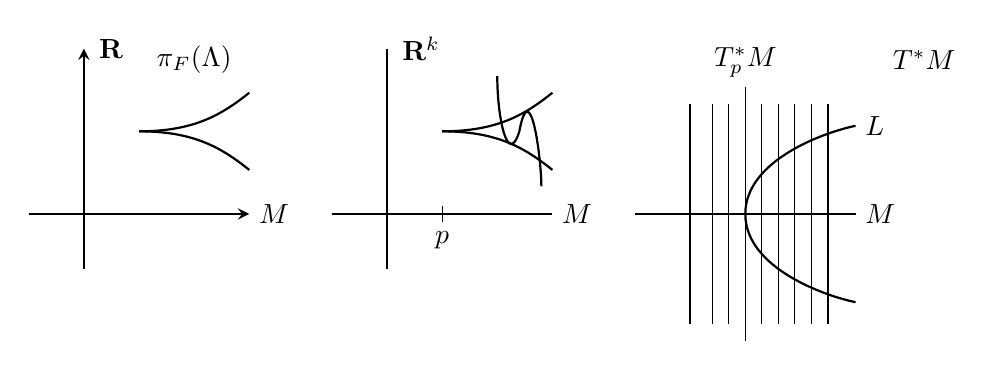
\begin{tikzpicture}[scale=.7]
%\draw[help lines=1,thin] (-5,-3) grid (5,3);
%\foreach \x in {-8,-6,...,8}\draw (\x,0) node{\x};
%\foreach \x/\y in {(0,1)/3,(0,0)/1,(0,-1)/2}
%\foreach \y in {-4,...,4}\draw (0,\y) node{\y};
%\coordinate (A) at (0,0);
%\draw[thick,color=blue] (A) ellipse [x radius=2.8cm,y radius=2.1cm];
\begin{scope}[xshift=-5.5cm]%sub
\draw[thick,-{stealth}] (-1,0)--(3,0);
\draw[thick,-{stealth}] (0,-1)--(0,3);
\draw (0.1,3) node[right]{$\bR$};
\draw (3,0) node[right]{$M$};
\draw (2,2.8) node{$\pi_F(\Lambda)$};
\draw[thick] (1,1.5)..controls (2,1.5) and (2.5,1.8)..(3,2.2);
\draw[thick] (1,1.5)..controls (2,1.5) and (2.5,1.2)..(3,0.8);
\end{scope}

\begin{scope}%sub
\draw[thick] (-1,0)--(3,0);
\draw[thick] (0,-1)--(0,3);
\draw (0.1,3) node[right]{$\bR^k$};
\draw (3,0) node[right]{$M$};
\draw[thick] (1,1.5)..controls (2,1.5) and (2.5,1.8)..(3,2.2);
\draw[thick] (1,1.5)..controls (2,1.5) and (2.5,1.2)..(3,0.8);
\draw[thick] (2,2.5)..controls (2,1.7) and (2.2,.85)..(2.4,1.5)..controls (2.6,2.55) and (2.8,1)..(2.8,.5);
\draw (1,-.15)--(1,.15);
\draw (1,-.15) node[below]{$p$};
\end{scope}

\begin{scope}[xshift=5.5cm]%sub
\draw[thick] (-1,0)--(3,0);
\draw[thick] (0,-2)--(0,2);
\foreach \x in {.4,.7,1,1.3,1.6,1.9,2.2,2.5}
\draw (\x,-2)--(\x,2);
\draw (1,-2.3)--(1,2.3);
\draw (1,2.3)node[above]{$T_p^\ast M$};
%\draw (0.1,3) node[right]{$\RR$};
\draw (3,0) node[right]{$M$};
\draw (3.5,2.8) node[right]{$T^\ast M$};
\draw[thick] (1,0)..controls (1,1) and (2.5,1.5)..(3,1.6);
\draw (3,1.6) node[right]{$L$};
\draw[thick] (1,0)..controls (1,-1) and (2.5,-1.5)..(3,-1.6);
\end{scope}

\end{tikzpicture}
\caption{The front projection $\pi_F(\Lambda) \subset M \times \bR$ of a Legendrian $\Lambda \subset J^1M$ near a cuspidal singularities is shown on the left. The realization of $\pi_F(\Lambda)$ as the Cerf diagram of a family of functions with moderate singularities is shown in middle. The corresponding Lagrangian $L \subset T^\ast M$ has moderate tangencies with respect to the foliation by fibers $T_q^*M$, $q \in M$, as shown on the right.}
\label{Figure1905}
\end{center}
\end{figure}
%
}
  
  In particular, when the front of a nearby Lagrangian homotopy sphere $\Sigma \subset T^*S^{4k}$ only has cusp type singularities, it is possible to compute tube torsion and nearby Lagrangian torsion of $\Sigma$ from the parametrized Morse theory of generating functions for $\Sigma$. A more precise version of this result will be stated and proved in Section \ref{sec: nearby} below.

  
  Next, we introduce some terminology to distinguish from the case in which nearby Lagrangian torsion isn't defined.


\begin{definition} We say that a Legendrian $\Lambda \subset J^1 M$ has {\em trivial tube torsion} when $\tau(\Lambda) =\text{im}(p)$. We say that a nearby Lagrangian $L \subset T^*M$ has {\em trivial nearby Lagrangian torsion} when $\nu(L)=\text{im}(p)$. \end{definition}


\begin{remark} If a nearby Lagrangian $L \subset T^*M$ has trivial tube torsion, then it automatically has trivial nearby Lagrangian torsion. \end{remark}

We may formulate the resulting obstruction to Legendrian and Hamiltonian isotopy to the zero section as follows:
 
 \begin{corollary} If a Legendrian $\Lambda \subset J^1M$ is Legendrian isotopic to the zero section, then it has trivial tube torsion. In particular, if a nearby Lagrangian $L \subset T^*M$ is Hamiltonian isotopic to the zero section, then it has trivial nearby Lagrangian torsion. \end{corollary}
 
 The famous nearby Lagrangian conjecture states that any nearby Lagrangian $L \subset T^*M$ is Hamiltonian isotopic to the zero section. The following question is therefore natural.
  
 \begin{question}\label{ques: nearby Lag}
Must a nearby Lagrangian $L \subset T^*M$ have trivial nearby Lagrangian torsion? 
\end{question}

An affirmative answer to this question would provide further evidence towards the nearby Lagrangian conjecture, whereas a negative answer would disprove it. Note that according to the nearby Lagrangian conjecture the Legendrian lift $\Lambda \subset J^1M$ of a nearby Lagrangian $L \subset T^*M$ would in particular  be Legendrian isotopic to $M$, though even this weaker form of the conjecture is not known. It seems conceivable that there could exist a nearby Lagrangian with trivial nearby Lagrangian torsion but nontrivial tube torsion, which would also disprove the nearby Lagrangian conjecture. 

\begin{remark}
The invariant $\nu(L)$ is an invariant of a {\em single} nearby Lagrangian $L \subset T^*M$. It is a parametrized torsion invariant of a family of acyclic chain complexes associated to $L$. The space of parameters is $M$, and for a single parameter $m \in M$ the relevant chain complex is (at least conjecturally) $CF^*(T_mM,L)$, see Section \ref{sec: hol}. However, we take the generating function viewpoint in the present article and use the fiberwise Morse complex $C_*(f_m)$ of a natural generating function $f$ for $L$ instead. The work by Courte and Porcelli \cite{CP25} gives a vanishing result for the parametrized higher torsion of a {\em family} of nearby Lagrangians $L_z \subset T^*M$,$z \in Z$, where for a single parameter the relevant chain complex is $CF^*(M,L_z)$ for $M \subset T^*M$ the zero section, though \cite{CP25} also takes the viewpoint of generating functions. The work \cite{CP25} is closer to a parametric generalization of the result \cite{AK} of vanishing of Whitehead torsion for a single nearby Lagrangian $L \subset T^*M$, which concerns $CF^*(M,L)$. Indeed, the invariants $\tau(L)$ and $\nu(L)$ have no {\em non-parametric} analogue; the fiber of a tube bundle is simply connected so its Whitehead group is trivial. It's possible the two viewpoints may be reconciled by some assembly type map.  
\end{remark}

In the broader class of Legendrians which are not necessarily lifts of nearby Lagrangians, we show that the theory of tube torsion is nontrivial in that Legendrians with nontrivial tube torsion abound. In fact, we establish the existence of Legendrians which have nontrivial tube torsion and which are diffeomorphic to the base, so that the conjectural triviality of tube torsion for nearby Lagrangians would in any case not follow from known constraints on the topology of nearby Lagrangians.

To formulate the precise statement, we will use the viewpoint of Waldhausen \cite{W82} where a fibration sequence $\cH_\infty \to \cT_\infty \to BG$ is constructed. Here $\cH_\infty$ is the space of stable h-cobordisms of a point (which classifies bundles of h-cobordisms of a disk up to stable equivalence), $\cT_\infty$ is the stable space of tubes (which classifies tube bundles up to stable equivalence), and $BG$ is the classifying space for stable spherical fibrations, so $G=\lim_n G_n$ for $G_n$ the space of self homotopy-equivalences of $S^n$. In particular, this means given a bundle $H \to V \to M$ of h-cobordisms of a disk, one may attach $V$ to a trivial tube bundle $M \times T$, where $T$ is the standard tube, to obtain a tube bundle $T \to W \to M$. The tube bundle $W$ has the same higher torsion as $V$. 

\begin{theorem}\label{thm: existence of example} 
Let $H \to V \to M$ be a bundle of $h$-cobordisms of a disk and let $T \to W \to M$ the resulting tube bundle. There exists a Legendrian $\Lambda \subset J^1M$ which admits a generating function on $W$ and whose projection to the base $\Lambda \to M$ is homotopic to a diffeomorphism. In particular the higher torsion classes $\tau_k(V) \in H^{2k}(M;\bR)$ of $V$ are contained in the tube torsion $\tau(\Lambda) \subset H^*(M;\bR)$ of $\Lambda$.
\end{theorem}

The higher torsion of tube bundles arising from h-cobordism bundles as in Theorem \ref{thm: existence of example} is in general not contained in the image of the (normalized) Pontryagin character, and hence this result shows that Legendrians with nontrivial tube torsion exist in abundance. Unfortunately, we do not know how to visualize a single explicit example of a Legendrian with nontrivial tube torsion. The simplest possible example would live in $J^1S^4$.

 \begin{problem}\label{pros: exhibit}
Describe explicitly, or draw the front of a Legendrian in $J^1S^4$ with nontrivial tube torsion.
\end{problem}

Although we do not know whether nearby Lagrangians must always have trivial tube torsion, or even whether they must always have trivial nearby Lagrangian torsion, in the upcoming work \cite{AIS} we will prove the triviality of nearby Lagrangian torsion under the additional assumption that the front admits a ruling satisfying certain technical conditions, which we call a {\em restricted ruling}.

Finally we note that if a nearby Lagrangian $L \subset T^*M$ has a stable Gauss map $L \to U/O$ which is not nullhomotopic, then it cannot admit any generating function, so that tube torsion is not defined. However, such an $L$ would already be a counterexample to the nearby Lagrangian conjecture, since a Hamiltonian isotopy between $L$ and the zero section would in particular yield a nullhomotopy of the stable Gauss map. 

\begin{comment}
Although we are not able to prove that nearby Lagrangians have trivial tube torsion in general, we do prove the triviality of tube torsion under the additional assumption that there exists a ruling satisfying certain technical conditions, which we call a {\em restricted ruling}. For $\Lambda \subset J^1M$ a Legendrian which admits a restricted ruling, a generating function for $\Lambda$ is constructed using the doubling construction (even if $\Lambda$ has Reeb chords), see Theorem \ref{thm: RulingGeneratingFamily}. We compute the higher torsion to be trivial for this specific generating function, from which we obtain the following conclusion.


\begin{theorem}\label{thm: VanishingTorsion}
Let $L \subset T^*M$ be a nearby Lagrangian. If $L$ admits a restricted ruling, then the nearby Lagrangian torsion $\nu(L)$ of $L$ is trivial.
\end{theorem}

If a nearby Lagrangian $L \subset T^*M$ has trivial stable Gauss map $L \to U/O$, then it admits a generating function on some tube bundle, and hence by a barcode construction one would expect it to be possible to equip its front with some higher dimensional generalization of the notion of a ruling. For example, in the case where $M$ is a homotopy sphere it was shown in \cite{AD22} that the h-principle for the simplification of caustics \cite{AG18a, AG18b} applies and hence after a Hamiltonian isotopy one may assume that the front of $L$ only has cusp singularities. Then the barcode pairs the sheets of the front according to some fixed rules imposed by Morse theory. However, in general there will be higher codimension bifurcations in the resulting ruling, going beyond the technical conditions imposed in our notion of a restricted ruling which in particular restricts the bifurcations of the ruling to be of low codimension. It is possible that the methods of this article may be extended to use the existence of this more general kind of ruling to prove vanishing of torsion for arbitrary nearby Lagrangians with stably trivial Gauss map. Or it could be that the methods encounter an obstacle, in the form of a higher dimension bifurcation of the ruling which contributes nontrivially to the torsion. In that case, perhaps that local computation of nontrivial nearby Lagrangian torsion could be used as guidance to construct a  counterexample to the nearby Lagrangian conjecture. 
\end{comment}

\subsection{Structure of the article}\label{sec: structure}
In Section \ref{sec: Reidemeister} we define a general class of invariants which we collectively call {\em Legendrian higher torsion}. In Section \ref{sec: tube} we specialize to a specific version tailored to the nearby Lagrangian conjecture, which we call {\em tube torsion}, and prove the existence of Legendrians which are diffeomorphic to the base and which have nontrivial tube torsion. In Section \ref{sec: nearby} we identify a distinguished coset of the tube torsion of a nearby Lagrangian, which we call {\em nearby Lagrangian torsion}, and prove that it is a Hamiltonian isotopy invariant. %In Section \ref{sec: vanishing} we prove vanishing of nearby Lagrangian torsion under the additional hypothesis of the existence of a restricted ruling. 
In Appendix \ref{sec: moderate singularities} we give some background on functions with moderate singularities and in  Appendix \ref{sec: higher torsion of bundles} we give some background on the definition of higher torsion invariants of fiber bundles.

\subsection{Acknowledgements}
We are grateful to Sander Kupers for private communication related to the numerical comparison of regulators and higher torsion. The first author is grateful for the support of the NSF under grant DMS-2203455, the Simons Foundation and the K-Theory foundation.  The second author is grateful for the support of the Simons Foundation, grant \# 686616. The third author is grateful for the support of the Simons Foundation, grant \# 019208.


\section{Legendrian higher torsion}\label{sec: Reidemeister}

In this section we present a general construction of Legendrian invariants using higher torsion classes, which are certain characteristic classes of fiber bundles of smooth manifolds arising from algebraic K-theory. %We keep the discussion as streamlined as possible but include  in Appendix \ref{sec: higher torsion of bundles}. 

\subsection{Fiber bundles and fibrations at infinity}
Let $M$ be a closed, connected smooth manifold. We consider fiber bundles of smooth manifolds $F \to W \to M$ and functions $f:W \to \bR$ on the total space, which we will often think of as families of functions $f_m:F_m \to \bR$ on the fiber $F_m \simeq F$, parametrized by $m \in M$. In the simplest case $F$ is a closed manifold. When $F$ is not a closed manifold we will have to add conditions to the possible functions $g:F \to \bR$ we consider. % In particular, we don't want critical points or gradient flows connecting them escaping to infinity in 1-parameter families. 
We use the terminology of \cite{EG98} in the following definition.


\begin{definition}
\label{def: Fibration at Infinity}
A function $f:F \to \bR$ is a  {\em fibration at infinity} if there exists a finite segment $[-a,a] \subset \bR$ and a compact subset $K \subset f^{-1}[-a,a] \subset F$ such that the restriction of $f$ to the following three subsets fibers them over their respective images:
\begin{enumerate}
\item $f^{-1}(-\infty,a] \to (-\infty,a]$
\item $f^{-1}[a,\infty) \to [a,\infty)$
\item $(f^{-1}[-a,a] ) \setminus K \to [-a,a]$
\end{enumerate}
\end{definition}

As noted in \cite[Section 0.2.1]{EG98}, a function $f:F \to \bR$ is a fibration at infinity if and only if $F$ admits a complete Riemannian metric with respect to which $\| df \| \geq \varepsilon>0$ outside of a compact subset.

\begin{example} The following are fibrations at infinity.
\begin{enumerate}
\item A non-degenerate quadratic form $q:\bR^N \to \bR$.
\item A function $f:\bR^N \to \bR$ of class $C^1$ which is 2-homogeneous, i.e. $f(\lambda v) = \lambda^2f(v)$, outside of a compact subset $K \subset \bR^N$ and such that the function $g:S^{N-1} \to \bR$ given by $g(v)=\lim_{\lambda \to +\infty} f(\lambda v)$ is a smooth function which has $0$ as a regular value. 
\item A function $f:\bR^N \to \bR$ which is a bounded $C^1$-distance from a function as in (2). 
\item The direct sum of two fibrations at infinity on the product domain.
\end{enumerate}
\end{example}

For a first contact with higher Reidemeister torsion it will be sufficient to consider, for $F$ a closed manifold, the class of fiber bundles $W \to M$ over $M$ whose fiber is diffeomorphic to $F$, together with their stabilizations. By the stabilization of a fiber bundle we will mean the fiberwise product with a trivial $\bR^{4N}$ bundle, which yields a new fiber bundle
$$ F \times \bR^{4N} \to W \times \bR^{4N} \to M.$$
On this bundle (with non-compact fibers) we distinguish the following class of functions.

\begin{definition}\label{def: class}
Given $M$ and $F$ closed, smooth manifolds and $F \to W \to M$ a fiber bundle, we denote by $\mathcal{S}(W)$ the class of all of functions $f:W \times \bR^{4N} \to \bR$ which are fibrations at infinity of the form
$$
f(w, x, y) = g(w) + \varepsilon(w,x,y) + \|x\|^2 - \|y\|^2, \qquad (w,x,y) \in W \times  \bR^{2N} \times \bR^{2N} 
$$
where $g:W \to \bR$ is a smooth function and $\varepsilon$ is a smooth function with compact support. Functions $f:W \times \bR^{4N} \to \bR$ in the class $\mathcal{S}(W)$ will be said to be {\em{admissible.}}
\end{definition}

\begin{remark} Note that if $f:W \times \bR^{4N} \to \bR$ is admissible then in particular with respect to any Riemannian metric on $W$ it remains a bounded $C^1$-distance from the standard fiberwise quadratic form: $$q(w, x,y) = \|x\|^2-\|y\|^2, \qquad (w,x,y) \in W \times  \bR^{2N} \times \bR^{2N}.$$ \end{remark}

\begin{remark}
If instead of starting with a fiber bundle of closed manifolds $F \to W \to M$ we started with a fiber bundle whose fiber $F$ has boundary (or is non-compact), then some fixed asymptotic behavior near the boundary (or at infinity) for the functions $g:W \to \bR$ as in the above definition should be specified. %For instance, one could consider functions on the trivial bundle $W=M \times \bR^{N+1}$ which are {\em linear-quadratic} at infinity, i.e. such that $f(m,x,z)=Q(x)+L(z)$ for $(m,x,z) \in M \times \bR^N \times \bR$ outside of a compact subset, where $Q$ is a non-degenerate quadratic form and $L$ is a non-degenerate linear function. 
\end{remark}






\begin{warning} We should really write $\mathcal{S}(\pi)$ for $\pi:W \to M$ the fibration but we will abuse notation and use $\mathcal{S}(W)$  instead of $\mathcal{S}(\pi)$ throughout. \end{warning} 


\subsection{The Legendrian invariant}\label{sec: Reid inv}
%Let $M$ and $F$ be closed, connected smooth manifolds and consider a fiber bundle $F \to W \to M$. We will give the construction of higher Reidemeister torsion invariants for such a fiber bundle, but the reader may easily adapt the construction to work in more general classes, where $F$ may be allowed to be noncompact and the class of functions is required to consist of fibrations at infinity which have some specific control on the behavior at infinity. 

%For example, if $F$ is a compact manifold with boundary $\partial F$, we could complete a collar $\partial F \times [0,1) \subset F$ to have a cylindrical end $\wh F =(\partial F \times (-\infty,0] ) \cup  F$ and if $t \in (-\infty,1)$ denotes the collar coordinate demand that all functions $f: \wh F \to \bR$ under consideration agree with the $t$ coordinate in the collar $ \partial F \times (-\infty,1)$. Or, if $\partial F$ is not connected, one could demand that on some components of $\partial F \times (-\infty, 1)$ the functions under consideration equal $-t$, and on some $+t$, and so on. 

%Indeed, we will later focus on a version  of the construction which is tailored to the setting of the nearby Lagrangian conjecture, and for this purpose it will be convenient to consider a class of fiber bundles with fiber $\bR^N$ and a specific class of fibrations at infinity on them with a specific behavior at infinity, of so-called {\em tube type} following the terminology of Waldhausen.



 Let us first consider the case where the fiber $F$ is closed.
 
% Either $F$ is closed or equipped with a reference fibration at infinity. Part of the data of $\cF$ is the notion of an admissible function $f:W \to \bR$, which when $F$ is noncompact will involve a control on the behavior of $f$ at infinity.
 % It could be the class of all fiber bundles with fiber a fixed manifold $F$, or perhaps some special subclass of such a class of fiber bundles. We may assume for concreteness that $F$ is closed, but we in fact allow for $F$ to be compact with boundary equipped with a reference fibration near the boundary, or even to be noncompact and equipped with a fixed reference fibration at infinity.% We consider functions $f:W \to \bR$ , which we will often think of as families of functions $f_m: \pi^{-1}(m) \to \bR$ on the fibers $\pi^{-1}(m) \simeq F$, parametrized by $m \in M$. 
 %and when $F$ is noncompact we will also demand control on the behavior of $f$ at infinity,  see Section \ref{} for details. %The notion of an admissible functions is also part of the class $\cF$. 
 %Fiber bundles $W \to M$ in $\cF$ will be equipped with a choice of unitary local system $\rho: \pi_1 W \to U(m)$ such that $H_*(F;\bC^\rho)$, the homology of the fiber with twisted coefficients, is a unipotent $\pi_1M$-module. 
 
 \begin{definition}
 A {\em torsion pair} $(W,\rho)$ consists of a fiber bundle $F \to W \to M$ and a unitary local system  $\rho : \pi_1 W \to U(1)$ such that $H_*(F;\bC^\rho)$ is a unipotent $\pi_1M$-module.
 \end{definition}
 
Here $H_*(F;\bC^\rho)$ denotes the homology of the fiber with the twisted complex coefficients given by $\rho|_{\pi_1F}$ and by {\em unipotent} we mean that the $\pi_1M$-module $H_*(F;\bC^\rho)$ admits a filtration by $\pi_1M$ submodules so that the action of $\pi_1M$ on the successive subquotients is trivial (a basepoint $b \in M$ should be chosen but this choice is immaterial). 
 
 \begin{warning}
We should really write $(\pi,\rho)$ for $\pi:W \to M$ the fibration but we will abuse notation and write $(W, \rho)$ instead of $(\pi, \rho)$ throughout. 
 \end{warning}
 
 Given a torsion pair $(W,\rho)$, one has its higher Reidemeister torsion, which consists of cohomology classes $\tau_k(W,\rho) \in H^{2k}(M;\bR)$, whose construction is reviewed in Appendix \ref{sec: higher torsion of bundles}. 
 
 By a {\em Legendrian submanifold} we will mean throughout a Legendrian embedding $\Lambda \hookrightarrow J^1M$ of a closed smooth manifold $\Lambda$, i.e. compact and without boundary. By an {\em immersed Legendrian} we will mean a Legendrian immersion $\Lambda \to J^1M$ of a closed smooth manifold $\Lambda$, though we will abuse notation and denote both embedded and immersed Legendrians by $\Lambda \subset J^1 M$. To make the connection between functions on fiber bundles over $M$ and Legendrians in $J^1M$ we need an additional condition on the functions we consider. The condition is generic, and is the standard definition of a {\em generating function} for a Legendrian in a 1-jet space. Recall that the {\em vertical differential} of a function $f:W \to \bR$ on the total space of a fiber bundle $\pi: W \to M$ is the restriction $d_vf$ of the usual differential $df:TW \to \bR$ to the vertical distribution $\ker(d \pi) \subset TW$. 

\begin{definition} A function $f:W \to \bR$ is said to be a {\em{generating function}} if the vertical differential $d_v f$ is transverse to zero. 
\end{definition}

If $f$ is a generating function, then $f$ determines a Legendrian immersion from the fiberwise singular locus $\Sigma_f = \{ d_v f = 0 \} \subset W$ into $J^1M$. Indeed, the condition that $d_v f \pitchfork 0$ means that the graph $\Gamma(df) \subset T^*W$ intersects transversely the coisotropic sumanifold $X \subset T^*W$ consisting of covectors which are zero on the fibers $T_mF$, $m \in M$. The symplectic reduction of the coisotropic submanifold $X$ is naturally identified with $T^*M$ and the image of the submanifold $X \cap \Gamma(df) =\Gamma(df)|_{\Sigma_f}$ under this reduction is an immersed exact Lagrangian submanifold of $T^*M$ whose Legendrian lift (via the values of $f$) is an immersed Legendrian submanifold $\Lambda \subset J^1M$.  

When moreover $\Lambda$ is an embedded Legendrian submanifold of $J^1M$ (which is the case generically), one says that the Legendrian submanifold  $\Lambda \subset J^1M$ is {\em generated} by $f$. %When $\Lambda$ is generated by $f$, the front projection of $\Lambda$, i.e. its image under the forgetful map $J^1M \to J^0M$, is the Cerf diagram $\{ (m, z) : \, \text{$z$ is a critical value of $f_m$} \} \subset M \times \bR$ of the family $f_m$. 

Now fix a collection $\cF$ of torsion pairs $(W,\rho)$. Examples of reasonable collections to consider include but are not limited to:
\begin{enumerate}
\item The singleton consisting of a fixed $W$ and a fixed $\rho$.
\item The collection of all $(W,\rho)$ for a fixed $W$ but all possible $\rho$ for that $W$. 
\item The collection of all possible torsion pairs $(W,\rho)$ with fiber a fixed closed manifold $F$.
\end{enumerate}

\begin{definition}  Let  $\Lambda \subset J^1M$ be a Legendrian submanifold. The {\em{Legendrian higher torsion}} of $\Lambda$ in the class $\cF$ is the subset $\tau(\Lambda,\cF) \subset H^*(M;\bR)$ consisting of all higher Reidemeister torsion classes $\tau_k(W,\rho) \in H^{2k}(M;\bR)$ of torsion pairs $(W,\rho)$ in $\cF$ such that $\Lambda$ admits a generating function $f \in \mathcal{S}(W)$.
\end{definition}

\begin{theorem}
If $\Lambda_0,\Lambda_1 \subset J^1M$ are Legendrian isotopic, then $\tau(\Lambda_0,\cF)=\tau(\Lambda_1,\cF)$. 
\end{theorem}

\begin{proof}As follows from the homotopy lifting property for generating functions under Legendrian isotopy up to stabilization, if $\Lambda_0$ admits a generating function in the class $\mathcal{S}(W)$, then so does $\Lambda_1$. The desired result then follows immediately. The homotopy lifting property for generating functions under Legendrian isotopies has a long history \cite{S86, C96}, but the formulation which is needed at this level of generality may be found in \cite{EG98}.
\end{proof} 


 %called the {\em higher Reidemeister torsion} of $\Lambda$ in the class $\cF$, which is a Legendrian isotopy invariant.  Roughly speaking, $\tau(\Lambda,\cF)=\coprod_k \tau_k(\Lambda,\cF)$, where $\tau_k(\Lambda,\cF) \subset H^{2k}(M;\bR)$ consists of union of the degree $2k$ higher Reidemeister torsion classes $\tau_k(W,\rho) \in H^{2k}(M;\bR)$ of all fibre bundles $W \to M$ which arise from stabilizations of fiber bundles in the class $\cF$ and on which $\Lambda$ admits a generating function $f:W \to \bR$. The specific choice of class of fiber bundles $\cF$ will depend on the concrete application in mind.
 
 \subsection{Suitable classes of fiber bundles}\label{sec: class}

Of course, given a Legendrian $\Lambda \subset J^1M$, for most choices of $\cF$ we will have $\tau(\Lambda)=\varnothing$, since many Legendrians don't admit any generating function and even those which do will only admit generating functions on certain fiber bundles. More generally, if one wishes to use generating function theory to study a particular class of Legendrians, then one should make a judicious choice for the class $\cF$ of fiber bundles and notion of admissible generating function under consideration.

As a first example, if $\Lambda$ is disjoint from a single fiber $T_xM \times \bR \subset J^1M$ then it won't admit a generating function on any fiber bundle $F \to W \to M$ with fiber $F$ a closed manifold, even after stabilization. In particular, if one wishes to study compact Legendrian submanifolds of $J^1\bR^n=\bR^{2n+1}$ one should consider a theory of generating functions with zero fiberwise Morse homology. In the $n=1$ case one could consider as in \cite{JT} generating functions $f:\bR \times \bR^{k+1}\to \bR$ on the trivial $\bR^{k+1}$-bundle over $\bR$ which are linear-quadratic at infinity, i.e. such that for $(w,v,z) \in \bR \times \bR^k \times \bR$ there holds outside of a compact subset $f(w,v,z)=Q(v)+L(z)$ for $Q$ a nondegenerate quadratic form and $L$ a nondegenerate linear form. 

If instead one is interested in studying Legendrian braids in $J^1S^1$, then one could consider  as in  \cite{T01} generating functions $f:S^1 \times \bR^k \to \bR$ on the trivial $\bR^k$-bundle over $S^1$ which are quadratic at infinity, i.e. such that for $(w,v) \in S^1 \times \bR^k$ there holds outside of a compact subset $f(w,v)=Q(v)$ for $Q$ a nondegenerate quadratic form.

Other classes of fiber bundles may be useful for other purposes. We explain the simplest example of a nontrivial application of the theory of Legendrian higher torsion known to us, in which the class of fiber bundles under consideration consists of circle bundles over orientable surfaces. In \cite{AI} the first two authors investigated a class of Legendrian submanifolds which admit generating functions on such circle bundles. Given an oriented circle bundle over an oriented surface $S^1 \to W \to \Sigma$, with Euler number $n\in \bZ$, and given a rank 1 unitary local system $\rho : \pi_1 W \to U(1)$ such that the oriented fiber $S^1$ gets sent to $u^{-1}$ for $u \neq 1$ an $n$-th root of unity, the higher Reidemeister torsion $\tau_1(W,\rho) \in H^2(\Sigma;\bR) \simeq \bR$ is a constant multiple of the Euler number of the circle bundle up to sign, as was computed by the second author and J. Klein in \cite{IK93a, IK93b}. Concretely, we have
$$ \tau_1(W,\rho) = n \, \,  \text{Im} \left(  \mathcal{L}_2(u)  \right) $$
where $\mathcal{L}_2$ is the dilogarithm
$$ \mathcal{L}_2(z) = \sum_{k=1}^\infty \frac{z^k}{k^2} .$$
That the higher Reidemeister torsion up to sign survives as a stable invariant of the circle bundle and is equal to the Euler class is a nontrivial fact. This fact is a special case of a deep result of B\"okstedt \cite{B82}, and may also be deduced from the theory of higher Reidemeister torsion, see \cite{I02}, concretely Chapter 7 (complexified B\"okstedt theorem). In  \cite{IK93a, IK93b} a more direct calculation for this special case is given. 


The class of Legendrians $\Lambda \subset J^1 \Sigma$ which were studied in \cite{AI} are called {\em mesh Legendrians}. Each mesh Legendrian $\Lambda$ is determined by combintarial data and admits an explicit generating function on a circle bundle of Euler number  $\pm e_\Lambda$ for a non-negative integer $e_\Lambda  \in \bZ_{\geq0}$ which is defined in terms of the combinatorial data. In \cite{AI} a calculation was carried out to determine the possible 2-parametric fiberwise Morse complex bifurcations that a generating function for the mesh Legendrian $\Lambda$ could support, on any such circle bundle over $\Sigma$. 

In particular it was shown that for any $n \in \bZ_{\geq 0}$ a mesh Legendrian $\Lambda$ only admits a generating function on the circle bundle $S^1 \to W \to \Sigma$ of Euler number $\pm n$ if $n=e_\Lambda$, {\em even after stabilization} of the circle bundle. Hence for  the singleton class $\cF=\{(W,\rho)\}$ consisting of a circle bundle  $S^1 \to W \to \Sigma$ of Euler number $\pm n$ and  $\rho : \pi_1 W \to U(1)$  a rank 1 unitary local system which sends the oriented fiber $S^1$ to $u^{-1}$ for $u \neq 1$ an $n$-th root of unity, the Legendrian higher torsion of a mesh Legendrian $\Lambda \subset J^1 \Sigma$ in the class $\cF$ consists of the singleton
 $$\tau_1(\Lambda,\cF)=\{ e_\Lambda \text{Im}( \mathcal{L}_2(u))  \} \subset H^2(\Sigma;\bR) \simeq \bR$$
 if $n=e_\Lambda$, and is empty otherwise. This proves:
 \begin{theorem}[implicit in \cite{AI}] The Legendrian higher torsion of a mesh Legendrian $\Lambda \subset J^1 \Sigma$ recovers (and uniquely determines) the Euler number (up to sign) of the unique circle bundle that may be used to generate it, even after stabilization of the tube bundle and/or Legendrian isotopy of $\Lambda$.  \end{theorem}
  %This computation in particular shows that a mesh Legendrian $\Lambda$ can only be generated on a circle bundle of Euler number $\pm e_\Lambda$, even after stabilization of the circle bundle or Legendrian isotopy of $\Lambda$. 

In fact in this specific situation the invariant can be refined to a Turaev type torsion which  is also sensitive to the sign of the Euler number,  and in this refined version the invariant was defined and used in \cite{AI} to distinguish Legendrian isotopy classes of mesh Legendrians in $J^1\Sigma$ in the same formal Legendrian class. The computations of \cite{AI} can be thought of as a proof of concept that higher torsion invariants may sometimes be calculated for explicit Legendrians. 

Our final example of a class $\cF$ of fiber bundles which one may want to consider for the definition of a Legendrian higher torsion invariant, and the most important class for the purposes of the present article, is the class of {\em tube bundles}. Roughly speaking, tube bundles are the most general class of fiber bundles on which one might hope to construct generating functions for {\em nearby Lagrangians}. Hence tube bundles provide the natural class of fiber bundles in which to define a Legendrian higher torsion invariant that may be relevant in the context of the  nearby Lagrangian conjecture. We discuss tube bundles and the associated Legendrian higher torsion invariant, which we call {\em tube torsion}, in Section \ref{sec: tube} below.

\subsection{Stable Gauss map} \label{sec: stable gauss map}

Given a Legendrian $\Lambda \subset J^1M$, for the Legendrian higher torsion to be defined, i.e. for $\tau(\Lambda,\cF)$ to be nonempty, in addition to the necessity of making a suitable choice for the class $\cF$ of fiber bundles (and unitary local systems) under consideration, it is also necessary that the stable Gauss map $\Lambda \to U/O$ is trivial, i.e. nullhomotopic Indeed, the triviality of the stable Gauss map is a necessary condition for the existence of {\em any} generating function, even in a very weak sense. Let us briefly recall the definition of the stable Gauss map.

 Let $\pi_{\text{Lag}} : J^1M = T^*M \times \bR \to T^*M$ denote the Lagrangian projection and consider the symplectic vector bundle $E=\pi_{\text{Lag}} ^*T(T^*M)|_\Lambda$ over $\Lambda$. Note that $E$ is equipped with two polarizations, i.e. Lagrangian sub-bundles, namely $G=T\Lambda$ (since $\pi_{\text{Lag}} |_\Lambda : \Lambda \to T^*M$ is a Lagrangian immersion) and $V=\pi_{\text{Lag}} ^*\nu|_\Lambda$, where $\nu$ is the Lagrangian distribution on $T^*M$ tangent to the fibers of the cotangent bundle projection $T^*M \to M$. The stable Gauss map measures the stable difference between these two polarizations. 
 
 Concretely, pick a Lagrangian sub-bundle $H$ of $E$ which is transverse to $V$, so that we have a isomorphism of symplectic vector bundles $E \simeq H \oplus H^*$ under which $V$ gets identified with $H^*$. There exists some real vector bundle $H'$ over $\Lambda$ such that $H \oplus H'$ is a trivial real vector bundle. Then $H' \oplus (H')^* \oplus E \simeq (H \oplus H') \oplus (H \oplus H')^*$ is isomorphic to a trivial symplectic vector bundle $\Lambda \times \bC^m$. The Lagrangian sub-bundle $H' \oplus G  \subset (H' \oplus (H')^*) \oplus E$ may thus be viewed as a Lagrangian sub-bundle of the trivial symplectic vector bundle $\Lambda \times \bC^m$, and hence gives a map $\Lambda \to U_m/O_m$. After letting $m \to \infty$ we get the stable Gauss map $\Lambda \to U/O$, which is easily verified to be independent of choices up to homotopy.  

We say that the stable Gauss map $\Lambda \to U/O$ of a Legendrian $\Lambda \subset J^1M$ is {\em trivial} when it is nullhomotopic. That the triviality of the stable Gauss map $\Lambda \to U/O$ is a necessary condition for $L$ to admit any kind of generating function was shown by Giroux in \cite{G90}. In particular, no matter what  the class of fiber bundles $\cF$ under consideration is, for  Legendrian higher torsion to be defined, i.e. for $\tau(\Lambda,\cF)$ to be nonempty, we must have that the stable Gauss map $\Lambda \to U/O$ is trivial. 

We will say that the front of Legendrian $\Lambda \subset J^1M$ has {\em moderate singularities} if the front projection $$\Lambda \hookrightarrow J^1M \to J^0M = M \times \bR$$ only has cusp singularities. This property is closely related to the triviality of the stable Gauss map. Indeed, for $\Lambda \subset J^1M$ a Legendrian with moderate singularities, consider the co-oriented hypersurface $(S,\nu)$ where $S \subset \Lambda$ is the locus of points whose front have a cusp and $\nu$ is the Maslov co-orientation of $S$ in $\Lambda$, see \cite{A}. For simplicity let us assume that $\Lambda$ is closed, connected and orientable. The co-oriented cycle $(S,\nu)$ determines a class in $H_{n-1}(\Lambda;\bZ)$, where $n=\dim \Lambda$, which is Poincar\'e dual to the Maslov class $\mu_1 \in H^1(\Lambda,\bZ)$. We have $\mu_1=0$ if and only if there exists a bounding chain for $(S,\nu)$, i.e. a collection of subdomains $\Omega_1, \ldots, \Omega_k \subset \Lambda$ with disjoint boundaries such that $\coprod_j \partial \Omega_j = S$ and for each component of $S$ realized as (part of) the boundary of $\Omega_j$ the Maslov-coorientation $\nu$ on this component agrees with the outwards pointing coorientation determined by $\Omega_j$. We then have:

\begin{proposition}\label{prop: simp stab triv}
Let $\Lambda$ be a closed, connected, smooth manifold and $\Lambda \subset J^1M$ a Legendrian embedding. If the front of $\Lambda$ has moderate singularities and if its Maslov class $\mu_1 \in H^1(\Lambda,\bZ)$ is trivial, then the stable Gauss map $\Lambda \to U/O$ is trivial. In fact, any bounding chain for the pair $(S,\nu)$ determines a homotopy class of nullhomotopy of the Gauss map $\Lambda \to U/O$. \end{proposition} 

\begin{proof}
When $\Lambda$ has the homotopy type of a sphere of dimension $>1$ we have $\mu_1=0$ for trivial reasons and the argument is given in \cite{AD22}. The general case may be proved by a similar line of reasoning, see \cite{B27} for details. \end{proof}

\begin{remark}
To be more precise, the statement of Proposition \ref{prop: simp stab triv} should be that any bounding chain determines a homotopy of Lagrangian distributions between the stabilizations of $G$ and $V$ in the stabilization of the symplectic vector bundle $E$, with notation as in the definition of the stable Gauss map above. So although the stable Gauss map $\Lambda \to U/O$ is only well-defined up to homotopy, we may still speak of a homotopy class of nullhomotopy of the stable Gauss map by defining this to be a homotopy of Lagrangian distributions between the stabilizations of $G$ and $V$. 
\end{remark}

Note that if $L \subset T^*M$ is a nearby Lagrangian, then the front of the Legendrian lift of $L$ has moderate singularities if and only if the tangencies of $L$ with respect to the foliation of $T^*M$ by the cotangent leaves $T^*_mM$, $m \in M$, has {\em quadratic} tangencies. When this is the case we will say that $L \subset T^*M$ has {\em moderate tangencies}. From Proposition \ref{prop: simp stab triv} and the fact that nearby Lagrangians always trivial Maslov class \cite{A12} it follows that any nearby Lagrangian with moderate tangencies has stably trivial Gauss map $L \to U/O$, and moreover there is a distinguished choice of homotopy class of nullhomotopy given any bounding chain for the cusp locus. 


\section{Legendrian tube torsion}\label{sec: tube}
  
  
In this section we focus on a specific version of Legendrian higher torsion which we call {\em Legendrian tube torsion}.

\subsection{Generating functions for nearby Lagrangians}\label{sec: gen fun nearby}

We recall that a nearby Lagrangian is an exact Lagrangian submanifold $L \subset T^*M$, where $L$ and $M$ smooth manifolds which are closed, connected and of the same dimension. The nearby Lagrangian conjecture states that any nearby Lagrangian is isotopic through nearby Lagrangians to the zero section.

For a nearby Lagrangian $L \subset T^*M$ to admit a generating function on a fiber bundle $F \to W \to M$, it is necessary that the fiberwise Morse homology of the generating function have Euler characteristic $\pm 1$. Indeed, the projection $L \to M$ is known to be a homotopy equivalence \cite{FSS, Na09, A12, Kra13, Gui12}, and in particular has degree $\pm 1$.% In particular we cannot hope to use fiber bundles with closed fibers; we must use non-compact fibers.

The most basic example to keep in mind is the trivial bundle $M \times \bR^{4N}$ with a generating function $f:M \times \bR^{4N} \to \bR$ which is equal to the standard fiberwise quadratic form $\|x\|^2-\|y\|^2$ outside of a compact subset, $(x,y) \in \bR^{2N} \times \bR^{2N}$. We will call such generating functions {\em standard quadratic at infinity}.  Note that the zero-section can be generated by such a function (namely the constant family of standard quadratic forms $F(m,x,y)=\|x\|^2-\|y\|^2$). Therefore, if the nearby Lagrangian conjecture is true, then by the homotopy lifting property for generating functions up to stabilization it would follow that any nearby Lagrangian admits a generating function standard quadratic at infinity. 


While existence of such generating functions for nearby Lagrangians is not known, there has been recent progress on existence of generating functions for nearby Lagrangians on the more general class of so-called {\em tube bundles}. The class of tube bundles is a class of fiber bundles which was introduced by Waldhausen in his manifold approach to the algebraic K-theory of spaces \cite{W82}. The precise definition of a tube bundle that we will work with in the present article will be given in Section \ref{sec: tube bundles} below, but let us note that in particular the fiberwise Morse homology of our notion of {\em generating function of tube type} has rank 1 concentrated in a single degree, just like a nondegenerate quadratic form.  The foundational result of the article \cite{ACGK} by Abouzaid, Courte, Guillermou and Kragh is the following. 

\begin{theorem}[\cite{ACGK}]\label{thm: existence generating functions tube}  A nearby Lagrangian $L \subset T^*M$ with trivial stable Gauss map $L \to U/O$ admits a generating function of tube type. \end{theorem}

So the condition that $L \to U/O$ is trivial, which as explained in Section \ref{sec: stable gauss map} is necessary for the existence of {\em any} kind of generating function, is in fact both necessary and sufficient for a nearby Lagrangian $L \subset T^*M$ to admit a generating function of tube type.  It is not known whether every nearby Lagrangian $L \subset T^*M$ must have stably trivial Gauss map. However, it was shown in \cite{ACGK} that if  $L \subset T^*M$ is a nearby Lagrangian, then $L \to U/O$ is trivial on homotopy groups.  In particular, if $M$ is a homotopy sphere, then any nearby Lagrangian $L \subset T^*M$ has stably trivial Gauss map and hence there holds:

\begin{theorem}[\cite{ACGK}] If $M$ is a homotopy sphere, then any nearby Lagrangian $L \subset T^*M$ admits a generating function of tube type. \end{theorem} 

Finally, the discussion at the end of Section 3 in \cite{ACGK}  (see the proof of Theorem 3.26 and preceding lemmas) makes it apparent that tube bundles are in some sense the most general class of fiber bundles on which one may expect a nearby Lagrangian to admit a generating function. The class of tube bundles therefore seems a reasonable class of fiber bundles to study in the context of the nearby Lagrangian conjecture, particularly in the case of nearby Lagrangian homotopy spheres. 

\subsection{Functions of tube type}\label{sec: tube bundles}

Rather than the model for tube bundles and functions of tube type used in \cite{ACGK} we  will use a convenient model for the space of tubes which was developed in work of the first author joint with Abouzaid, Courte and Kragh in \cite{AACK}. That Theorem \ref{thm: existence generating functions tube} also holds for this model was proved in \cite{AACK}. First we will need to introduce a few preliminary notions. 

\begin{definition}\label{def: quad tube}
A $C^1$-function $g:\bR^N \to \bR$ is a {\em{function of quadratic tube type}} if it satisfies the following:
\begin{enumerate}
\item $g$ is homogeneous of degree 2, i.e. $g(\lambda v) = \lambda^2 g(v)$.
\item $g$ has no critical point other than the origin.
\item $g$ is homotopic through functions satisfying (1) and (2) to a non-degenerate quadratic form. 
\end{enumerate}
\end{definition}

Note that in general the homogenization of a smooth function $h:S^{N-1} \to \bR$, i.e. $g(v)=\|v\|^2h(v/\|v\|)$ for $v \neq 0$ and $g(0)=0$, will only be of class $C^1$. 

\begin{definition}\label{def: tube}
A smooth function $f:\bR^N \to \bR$ is a {\em function of tube type} if there exists a function of quadratic tube type $g:\bR^N \to \bR$ such that $\| \nabla f - \nabla g \| \leq C$ for some constant $C>0$.
\end{definition}

\begin{remark} Note that if $g$ exists, then it is uniquely determined by $f$, indeed $g(v) = \lim_{\lambda \to \infty}  \frac{1}{\lambda^2}f(\lambda v)$. \end{remark}

Let $\cT_{k,N}^q$ denote the space of functions of quadratic tube type on $\bR^N$ such that the non-degenerate quadratic form in condition (3) has index $k$, and let $\cT_{k,N}$ be the space of functions of tube type on $\bR^N$ such that the associated function of quadratic tube type is in $\cT_{k,N}^q$. We also denote:
$$ \cT^q_N = \coprod_{k=0}^N \cT^q_{k,N}, \quad \cT^q = \coprod_{N=0}^\infty \cT^q_N , \quad \cT_N = \coprod_{k=0}^N \cT_{k,N}, \quad \cT = \coprod_{N=0}^\infty \cT_N. $$
Note that if $f_i:\bR^{N_i} \to \bR$ is a function of tube type for $i=1,2$, then $f_1 \oplus f_2 : \bR^{N_1} \times \bR^{N_2} \to \bR$ is also of tube type, so we have an operation $\cT_{k_1,N_1} \times \cT_{k_2,N_2} \mapsto \cT_{k_1+k_2,N_1+N_2}$ which endows $\cT$ with the structure of a topological monoid. We also have the topological submonoid of functions of quadratic tube type $\cT^q \subset \cT$.  Clearly the inclusion $\cT^q \subset \cT$ is an equivalence as the linear interpolation $(1-t)f+tg$ of a function of tube type $f$ with its associated function of quadratic tube type $g$ gives a deformation retraction of $\cT$ onto $\cT^q$.

We also denote $\cQ_{k,N}$ for the space of non-degenerate quadratic forms $q:\bR^N \to \bR$ of index $k$ and
$$ \cQ_N = \coprod_{k=0}^N \cQ_{k,N} , \qquad \cQ= \coprod_{N=0}^\infty \cQ_N. $$
Note that $\cQ_{k,N} \subset \cT_{k,N}^q$, and that $\cQ$ is a submonoid of $\cT^q$ and hence also of $\cT$.   %Let us denote by $\cT_N$ the space of all functions $f:\bR^N \to \bR$ of tube type and set $\cT= \coprod_N \cT_N$, which is a monoid under direct sum. We also denote by $\cQ_N$ the space of all non-degenerate quadratic forms $q: \bR^N \to \bR$ and set $\cQ=\coprod_N \cQ_N$. Note that $\cQ$ is a submonoid of $\cT$. 

\begin{definition}
Let $M$ be a closed, connected, smooth manifold.
\begin{enumerate}
\item A {\em{fibered function of tube type}}  is a smooth function $f:M \times \bR^N \to \bR$ such that for each $m \in M$ the restriction $f_m : \bR^N \to \bR$ is of tube type, i.e. such that $f_m \in \cT_N$ for each $m \in M$. 
\item A {\em{fibered function of quadratic tube type}}  is a $C^1$ function $f:M \times \bR^N \to \bR$ such that for each $m \in M$ the restriction $f_m : \bR^N \to \bR$ is quadratic of tube type, i.e. such that $f_m \in \cT_N^q$ for each $m \in M$. 
\item A {\em{fibered function of rigid tube type}}  is a smooth function $f:M \times \bR^N \to \bR$ such that for each $m \in M$ the restriction $f_m : \bR^N \to \bR$ is a non-degenerate quadratic form, i.e. if $f_m \in \cQ_N$ for each $m \in M$. 
\end{enumerate}
\end{definition}

\begin{remark} Since $M$ is connected, the index $k$ of any such fibered function of tube type is well-defined. \end{remark}

%\begin{remark} In particular, to a fibered function of tube type over $M$ is associated a continuous map $M \to \cT$, but there is the additional condition that the function defined on the total space $M \times \bR^N$ is smooth. \end{remark}

To a fibered function of tube type $f:M \times \bR^N \to \bR$ we may associate the fibered function of quadratic tube type $g:M \times \bR^N \to \bR$ such that for each $m \in M$ the restriction $g_m:\bR^N \to \bR$ is the function of quadratic tube type associated to the restriction $f_m:\bR^N \to \bR$. 

Fibered functions of tube type over $M$ form a monoid. Fibered functions of quadratic tube type over $M$ form submonoid of the monoid of fibered functions of tube type over $M$, and fibered quadratic functions of rigid tube type form yet a smaller submonoid. 


%The map which assigns to a $j$-dimensional vector subspace $E \subset \bR^k$ the orthogonal quadratic form $Q_E:\bR^k \to \bR$ with $+1$ eigenspace $E$ and $-1$ eigenspace $E^\perp$ yields a homotopy equivalence between the disjoint union of Grassmannians $BO(j,k)$ and the space of nondegenerate quadratic forms on $\bR^k$. In particular we may identify fibered functions of rigid tube type up to stabilization and up to homotopy through such with stable isomorphism classes of vector bundles over $M$. 
We will reserve the following terminology for the monoid operation on fibered functions of tube type when one of the two functions is rigid. 

\begin{definition}
\label{def: TwistedSister}
Let $f:M \times \bR^{N_1} \to \bR$ be a fibered function of tube type and let $q:M \times \bR^{N_2}\to \bR$ be a fibered function of rigid tube type. We call $f\oplus q:M \times \bR^{N_1} \times \bR^{N_2} \to \bR$ the {\em{twisted stabilization}} of $f$ by $q$. 
\end{definition}

By a {\em{stabilization}} without the adjective {\em twisted} we will mean a stabilization with respect to a constant fibered function of rigid tube type $q:M \times \bR^N \to \bR$, i.e. $q(x,v)=Q(v)$ for some fixed non-degenerate quadratic form $Q: \bR^N \to \bR$. In fact, typically we will stabilize by the standard form on $\bR^4$ given by  $q(x,y)=\|x\|^2-\|y\|^2$ for $(x,y) \in \bR^{2} \times \bR^{2}$, and will refer to such a stabilization as a {\em standard stabilization}. 


\begin{definition}
Let $q:M \times \bR^N \to \bR$ be a fibered function of rigid tube type, so that $q(m,x)=Q_m(x)$ for $Q_m:\bR^N \to \bR$ a family of non-degenerate quadratic forms. Let $E \to M$ be the real vector bundle whose fiber $E_m$ over $m \in M$ is the negative eigenspace of the matrix $(\partial^2 Q_m/\partial x_i\partial  x_j)_{i,j}$. We call $E \to M$ the {\em stable bundle} of $Q$.
\end{definition}

\begin{remark}
Alternatively, a fibered function of ridid tube type is classified by a map $M \to \cQ$, the notion of stable bundle for a non-degenerate quadratic form determines a map $\cQ_{k,N} \to BO(k,N)$, and hence the stable bundle of a fibered function of ridid tube type is classified by the composition $M \to \cQ \to \bZ \times BO$. Note that the map $\cQ_{k,N} \to BO(k,N)$ is a homotopy equivalence, with homotopy inverse the map $BO(k,N) \to \cQ_{k,N}$ which sends a vector subspace $E \subset \bR^N$ of dimension $k$ to the quadratic form $Q(x)=\|x_{E^\perp} \|^2-\|x_E \|^2$, where $x=x_E+x_{E^\perp}$ is the decomposition of $x \in \bR^N$ into its $E$ and $E^{\perp}$ components.
\end{remark}


\subsection{Torsion of fibered functions of tube type}


Note that the second condition in Definition \ref{def: quad tube} is equivalent to asking that $g$ is transverse to zero outside of the origin, so for a function of quadratic tube type $g:\bR^N \to \bR$ the set $T(g)=\{g \leq 0 \} \cap S^{N-1}$ is a codimension-zero submanifold of $S^{N-1}$ (a priori only $C^1$, but $C^1$ submanifolds have unique smoothings up to contractible choice of isotopy). By the third condition of Definition \ref{def: quad tube} this submanifold is isotopic in $S^{N-1}$ to $T(q)=\{ q \leq 0 \} \cap S^{N-1}$ for $q$ a non-degenerate quadratic form. If $E^-$ is the negative eigenspace of $q$, then this domain is a tubular neighborhood of the equator $E^- \cap S^{N-1}$ and in particular is diffeomorphic to $S^{k-1} \times D^{N-k}$ for $k$ the index of $q$ and $D^m=\{ \|x\| \leq 1\} \subset \bR^m$ the unit disk. 

\begin{definition}
A {\em{rigid tube}} is the codimension zero submanifold $T(q) \subset S^{N-1}$ for $q$ a non-degenerate quadratic form. The {\em index} of a rigid tube is the index of $q$.
\end{definition}

\begin{definition} A {\em tube} is a codimension zero submanifold $T \subset S^{N-1}$ which is isotopic in $S^{N-1}$ to a rigid tube. The {\em index} of a tube is the index of any rigid tube it is isotopic to.
\end{definition}



{
%
\begin{figure}[htbp]
\begin{center}
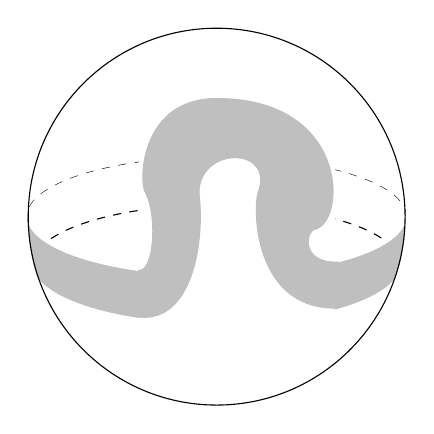
\begin{tikzpicture}[scale=1.5]
%\draw[help lines=1,thin] (-2,1) grid (4,6);
%\foreach \x in {-8,-6,...,8}\draw (\x,0) node{\x};
%\foreach \x/\y in {(0,1)/3,(0,0)/1,(0,-1)/2}
%\foreach \y in {1,...,6}\draw (0,\y) node{\y};
%\coordinate (A) at (0,0);
%\draw[thick,color=blue] (A) ellipse [x radius=2.8cm,y radius=2.1cm];
\begin{scope}% small sphere
\clip (1,4) circle[radius=1.6cm];
\draw[dashed,thick](1,4) ellipse[x radius=1.6cm,y radius=.5cm];
\draw[fill,gray!50!white] (1,3.6) ellipse[x radius=1.55cm,y radius=.5cm];
\draw[fill,gray!50!white] (1,3.8) ellipse[x radius=1.7cm,y radius=.5cm];
\draw[fill,white] (1,4) ellipse[x radius=1.6cm,y radius=.5cm];
\begin{scope}
\clip (-.5,3.8) rectangle (2.4,4.8);
\draw[dashed] (1,3.6) ellipse[x radius=1.55cm,y radius=.5cm];
\end{scope}
\draw[fill,white] (.35,3) rectangle (2,4.6);
%\draw[thick,red] (.34,3.545)..controls(.47,3.53)and(.5,4)..(.4,4.2)..controls (.34,4.27) and (.34,5)..(1,5)..controls (2.1,5) and (2.1,4)..(1.85,3.9)..controls (1.75,3.9) and (1.7,3.6)..(2.1,3.615);
\draw[fill,gray!50!white] (.34,3.15)..controls(.8,3.1)and(.9,3.8)..(.85,4.2)..controls(.85,4.6)and(1.5,4.6)..(1.35,4.2)..controls (1.3,4)and(1.35,3.2)..(2.03,3.227)--(2.03,3.615)..controls(1.7,3.6) and (1.75,3.9)..(1.85,3.9)..controls (2.1,4) and (2.1,5)..(1,5)..controls (.34,5)and(.34,4.27)..(.4,4.2)..controls (.5,4)and(.47,3.53)..(.34,3.545)--(.34,3.15);
\draw[thick] (1,4) circle[radius=1.6cm];
\end{scope}

%
\end{tikzpicture}
\caption{A tube $T \subset S^{N-1}$.}
\label{Figure1909}
\end{center}
\end{figure}
%
}

{
%
\begin{figure}[htbp]
\begin{center}
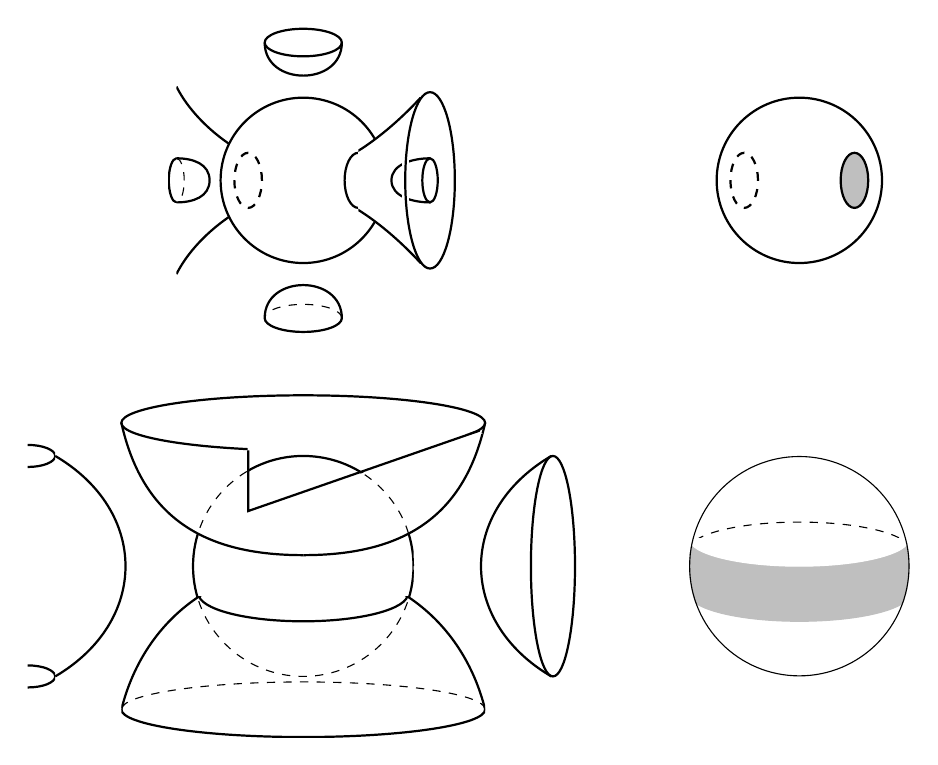
\begin{tikzpicture}[scale=.7]
%\coordinate (A) at (0,0);
%\draw[thick,color=blue] (A) ellipse [x radius=2.8cm,y radius=2.1cm];
%
\begin{scope}[xshift=9cm]% rigid tube, index 1
%
\clip (0,0) circle[radius=2cm];
\draw[dashed] (0,.3) ellipse[x radius=2cm,y radius=5mm];
\draw[fill,gray!50!white] (0,-.5) ellipse[x radius=2cm,y radius=5mm];
\draw[fill,gray!50!white] (-2,-.5)rectangle(2,.5);
\begin{scope}
\clip (-2,-.5)rectangle(2,.51);
\draw[fill,white] (0,.5) ellipse[x radius=2cm,y radius=5mm];
\end{scope}
\draw[thick] (0,0) circle[radius=2cm];
\end{scope}
%
\begin{scope}[xshift=9cm, yshift=7cm] % rigid tube, index 0
\draw[thick] (0,0) circle[radius=1.5cm];
\draw[fill,gray!50!white] (1,0)ellipse[x radius=2.5mm,y radius=5mm];
\draw[thick](1,0)ellipse[x radius=2.5mm,y radius=5mm];
\draw[dashed,thick] (-1,0)ellipse[x radius=2.5mm,y radius=5mm];
\end{scope}
%
{
\begin{scope}[yshift=7cm] % 3-D top
%\draw[help lines=1,thin] (-3,-3) grid (3,3);
%\foreach \y in {-3,...,3}\draw (0,\y) node{\y};
\begin{scope}
%\draw[fill,gray!50!white] (1,0)ellipse[x radius=2.5mm,y radius=5mm];
\draw[thick](1,0)ellipse[x radius=2.5mm,y radius=5mm];
\draw[fill,white] (1,-.6) rectangle (1.3,.6);
\draw[dashed,thick] (-1,0)ellipse[x radius=2.5mm,y radius=5mm];
\draw[thick] (0,0) circle[radius=1.5cm];
\end{scope}
%
\begin{scope}
\clip (1,-1.5)rectangle(2.4,1.5);
\draw[fill,white] (0,.2)..controls (.8,.15) and (1.9,1.2)..(2.3,1.7)--(2.3,-1.7)..controls (1.9,-1.2) and (.8,-.15)..(0,-.2);
%
\draw[thick] (0,.2)..controls (.8,.15) and (1.9,1.2)..(2.3,1.7);
\draw[thick] (0,-.2)..controls (.8,-.15) and (1.9,-1.2)..(2.3,-1.7);
%\draw[dashed] (0,0) circle[radius=1.5cm];
%\draw[dashed](1,0)ellipse[x radius=2.5mm,y radius=5mm];
\end{scope}

\begin{scope}
\draw[thick] (2.3,0) ellipse[x radius=1.4mm, y radius=4mm];
\draw[thick] (2.3,.4)..controls (2,.4) and (1.6,.3)..(1.6,0)..controls (1.6,-.3) and (2,-.4)..(2.3,-.4);
\draw[fill,white] (1.8,-.44)rectangle(1.9,.44);
\draw[thick] (2.3,0) ellipse[x radius=4.5mm,y radius=16mm];
\end{scope}

%
\begin{scope}
\clip (-2.3,-1.75)rectangle (-1.35,1.75);
\draw[thick] (0,.2)..controls (-.8,.15) and (-1.9,.9)..(-2.3,1.7);
\draw[thick] (0,-.2)..controls (-.8,-.15) and (-1.9,-.9)..(-2.3,-1.7);
\end{scope}

\begin{scope}
\draw[dashed] (-2.3,0) ellipse[x radius=1.4mm, y radius=4mm];
\draw[thick] (-2.3,.4)..controls (-2,.4) and (-1.7,.3)..(-1.7,0)..controls (-1.7,-.3) and (-2,-.4)..(-2.3,-.4);
\clip (-2.45,-.41) rectangle (-2.3,.41);
\draw[thick] (-2.3,0) ellipse[x radius=1.4mm, y radius=4mm];
\end{scope}

\begin{scope}
\draw[thick] (0,2.5) ellipse[x radius=7mm,y radius=2.5mm];
\draw[thick] (-.7,2.5)..controls (-.7,1.7) and (.7,1.7).. (.7,2.5);
\end{scope}

\begin{scope}
\draw[dashed] (0,-2.5) ellipse[x radius=7mm,y radius=2.5mm];
\draw[thick] (-.7,-2.5)..controls (-.7,-1.7) and (.7,-1.7).. (.7,-2.5);
\end{scope}
\clip (-.75,-5)rectangle (.75,-2.5);
\draw[thick] (0,-2.5) ellipse[x radius=7mm,y radius=2.5mm];

\end{scope}
}
%
{
\begin{scope}%[yshift=-5cm]% 3D bottom
\draw[dashed] (0,0) circle[radius=2cm];
%\draw[dashed] (0,.5) ellipse[x radius=1.9cm, y radius=5mm];

\begin{scope}
\clip (-3.3,-2.61)rectangle(3.3,-.55);
\draw[thick] (0,0)..controls (1.6,0) and (2.9,-1)..(3.3,-2.6);
\draw[thick] (0,0)..controls (-1.6,0) and (-2.9,-1)..(-3.3,-2.6);
\draw[thick] (0,-.5) ellipse[x radius=1.9cm, y radius=5mm];
\draw[dashed] (0,-2.6) ellipse[x radius=33mm,y radius=5mm];
\end{scope}

\begin{scope}
%\clip (-3.3,-2.61)rectangle(3.3,-.55);
\draw[thick] (0,0.2)..controls (1.7,0.2) and (2.9,.8)..(3.3,2.6);
\draw[thick] (0,0.2)..controls (-1.7,0.2) and (-2.9,.8)..(-3.3,2.6);
%\draw[thick,red] (0,.5) ellipse[x radius=1.9cm, y radius=5mm];
%\draw[dashed] (0,-2.6) ellipse[x radius=33mm,y radius=5mm];
\end{scope}

\begin{scope}
\clip (-3.3,-2.6)rectangle (3.3,-3.1);
\draw[thick] (0,-2.6) ellipse[x radius=33mm,y radius=5mm];
\end{scope}

\begin{scope}
\draw[thick] (0,2.6) ellipse[x radius=33mm,y radius=5mm];
\end{scope}

\begin{scope}
\clip (-2.1,-.55)rectangle(2.,.58);
\draw[thick] (0,0) circle[radius=2cm];
\end{scope}

\begin{scope}
\draw[fill,white] (-1,2.1)--(-1,1)--(3.2,2.4)--(-1,2.4)--cycle;
%(-1,1.5)rectangle(1.5,2.5);
\draw[thick] (-1,2.1)--(-1,1)--(3.2,2.46);
\clip (-1,2.1)--(-1,1)--(3.2,2.4)--(-1,2.4)--cycle;
\draw[thick] (0,0) circle[radius=2cm];
\end{scope}

\draw[thick] (-4.5,2)..controls (-2.8,1)and(-2.8,-1)..(-4.5,-2);

\draw[thick] (4.5,2)..controls (2.8,1)and(2.8,-1)..(4.5,-2);
\draw[thick] (4.53,0) ellipse[x radius=4mm,y radius=2cm];

\begin{scope}[xshift=-5mm]
\clip (-4.5,-2.5) rectangle (-4,-1.5);
\draw[thick] (-4.5,-2) ellipse[x radius=5mm,y radius=2mm];
\end{scope}

\begin{scope}[yshift=4cm,xshift=-5mm]
\clip (-4.5,-2.5) rectangle (-4,-1.5);
\draw[thick] (-4.5,-2) ellipse[x radius=5mm,y radius=2mm];
\end{scope}


\end{scope} % end 3D bottom
}
%
\end{tikzpicture}
\caption{Level sets of standard quadratic forms and corresponding rigid tubes.}
\label{Figure1910}
\end{center}
\end{figure}
%
}
\begin{definition}
A  {\em{tube bundle}} is a fiber bundle $W \to M$ over a smooth manifold $M$ such that 
\begin{enumerate}
\item $W$ is a codimension zero submanifold of $M \times S^{N-1}$
\item the map $W \to M$ is the restriction to $W$ of the projection $M \times S^{N-1} \to M$.
\item for each $x \in M$ the fiber over $x$ is a  tube $T_x \subset S^{N-1}$.
\end{enumerate}
\end{definition}

If for each $x \in M$ the fiber of a tube bundle $W \to M$ is a rigid tube $T_x=T(q_x) \subset S^{N-1}$, where $q_x:\bR^N \to \bR$ is a family of nondegenerate quadratic forms, then we call $W$ a {\em{rigid tube bundle.}} If $g: M \times \bR^N \to \bR$ is a fibered function of quadratic tube type, then we will denote by $T(g) \to M$ the associated tube bundle $T(g)=\{ g \leq 0\} \cap S^{N-1}$. If $f:M \times \bR^N \to \bR$ is a fibered function of tube type, we will denote $T(f)=T(g)$ the tube bundle associated to the underlying fibered function of quadratic tube type $g$. 

\begin{warning}
If $f:\bR^N \to \bR$ is a function of tube type, then $T(f)$ is not $\{ f \leq 0\} \cap S^{N-1}$. It is $\{ g \leq 0\} \cap S^{N-1}$ for $g(x) = \|x\|^2 \lim_{ \lambda \to \infty} f(\lambda x)$. The same comment applies (fiberwise) for fibered functions of tube type $f:M \times \bR^N \to \bR$ and their associated tube bundle $T(f) \to M$.
\end{warning}

\begin{definition}
\label{def: OrientedTubeBundle}
We will say that a tube bundle $W \to M$ of index $k$ is {\em orientable} if the action of $\pi_1 M$ on the homology of the fiber $H_{k-1}(T;\bZ) \simeq \bZ$ is trivial. 
\end{definition}

If $W \to M$ is an orientable tube bundle, then the action of $\pi_1M$ on the homology $H_*(F)$ of the fiber is trivial and hence in particular unipotent, so we may associate to $W$ its higher Reidemeister torsion classes $\tau_k(W) \in H^{2k}(M;\bR)$. We emphasize that for orientable tube bundles, no unitary local system is needed. As explained in Appendix \ref{sec: higher torsion of bundles}, this causes the classes in degrees congruent to 2 modulo 4 to be automatically trivial. So $\tau_{2k+1}(W)=0$ in $H^{4k+2}(M;\bR)$ and we are left with the classes $\tau_{2k}(W) \in H^{4k}(M;\bR)$. 

Recall that a fibered function of tube type $f:M \times \bR^{N} \to \bR$ has an associated fibered function of quadratic tube type $g:M \times \bR^{N} \to \bR$ and a corresponding tube bundle $W=T(f)=T(g)$ pver $M$.
\begin{definition} Let $f:M \times \bR^N \to \bR$ be a fibered function of tube type, with an associated fibered function of quadratic tube type $g:M \times \bR^N \to \bR$ and a corresponding tube bundle $W=T(g)$. If $W$ is orientable, then $f$ is called an {\em orientable} fibered function of tube type.\end{definition}

To an  oriented fibered function of tube type we may associate to $f$ the higher torsion classes $\tau_k(W)$ of the oriented tube bundle $W=T(g)$. These classes are invariant under homotopy of $f$ through oriented fibered functions of tube type. For $q:M \times \bR^N \to \bR$ a fibered function of rigid tube type, being orientable amounts to asking that the stable bundle $E \to M$ of $q$ is orientable.

Let us record the following basic fact.

\begin{lemma} Let $W_1=T(f_1)$ and $W_2=T(f_2)$ be tube bundles associated to orientable fibered functions of tube type $f_1:M \times \bR^N \to \bR$ and $f_2:M \times \bR^N \to \bR$. If $f_1$ is homotopic to $f_2$ through fibered functions of tube type, then $W_1$ and $W_2$ have the same higher torsion classes. \end{lemma}

\begin{proof} Such a homotopy $f_t$ yields an isotopy of codimension zero submanifolds $W_t=T(f_t)$ of $M \times S^{N-1}$ and hence by isotopy extension a fibered diffeomorphism $W_1 \simeq W_2$ of tube bundles over $M$. Higher torsion classes are invariant under fibered diffeomorphism. \end{proof}


If $f:M \times \bR^{N_1} \to \bR$ is an orientable fibered function of tube type and $q:M \times \bR^{N_2} \to \bR$ is an orientable fibered function of rigid tube type, then $f \oplus q:M \times \bR^{N_1+N_2} \to \bR$ is an orientable fibered function of tube type. Indeed for $k_1$ the index of $f$ and $k_2$ the index of $q$ we have $\Sigma T(g \oplus q) \simeq \Sigma T(g) \land \Sigma T(q)$ as $S^{k_1+k_2}$-fibrations over $M$ and hence $$H^{k_1+k_2-1}(T(g \oplus q)_m ;\bR) \simeq H^{k_1-1}(T(g)_m;\bR) \otimes H^{k_2-1}(T(q)_m;\bR)$$
Hence if both the rank 1 real vector bundles $H^{k_1-1}(T(g)_m;\bR)$ and $H^{k_2-1}(T(q)_m;\bR)$ over $M$  are trivial, then so is $H^{k_1+k_2-1}(T(g \oplus q)_m ;\bR)$. At this point it is not yet clear how the higher torsion of $T(g)$ and $T(g \oplus q)$ should be related. For this purpose we introduce a computational tool. 

If an orientable fibered function of tube type $f:M \times \bR^{N} \to \bR$ has {\em moderate singularities} (i.e. Morse or Morse birth/death, see Appendix \ref{sec: moderate singularities}), then it is possible to compute the resulting higher torsion classes from the parametrized Morse theory of $f$ directly, and this will be useful to us in what follows. We use the same notation as in the statement of the {\em framing principle} given in Theorem \ref{thm: framing}. We recall briefly the relevant notions:
\begin{enumerate}
\item $\tau_k(f)$ is a cohomology class in $H^{2k}(M;\bR)$ obtained from the family $C_*(f_m)$, $m \in M$, of Morse chain complexes for the fiberwise restrictions $f_m: \bR^{N} \to \bR$, $m \in M$.
\item $\gamma_f$ is a stable real vector bundle over the fiberwise singular set $\Sigma_f \subset M \times \bR^{N}$ formed by the negative eigenspaces of the fiberwise Hessian of $f$. 
\item $\pi_*^{\Sigma f}$ is the push-down operator in cohomology $H^*(\Sigma_f) \to H^*(M)$ induced by $\pi|_{\Sigma_f} : \Sigma_f \to M$.
\item for $E \to X$ a real vector bundle over a manifold $X$, $p_k(E)  \in H^{4k}(M;\bR)$ is the normalized Pontryagin character:
$$p_k(E) = \frac{1}{2}(-1)^k  \zeta(2k+1)ch_{2k}(E\otimes \bC) .$$
\end{enumerate}

\begin{remark}
To simplify issues with signs, from now on we will restrict to the case of even index and ambient dimension a multiple of four. Standard stabilization is by $\bR^4$ with the quadratic form $\|x\|^2-\|y\|^2$, $(x,y) \in \bR^2 \times \bR^2$, which will preserve higher torsion, including its sign. 
\end{remark}

\begin{proposition}\label{prop: stab framing}
Let $f:M \times \bR^{4N} \to \bR$ be an orientable fibered function of tube type with moderate singularities, with associated fibered function of quadratic tube type $g:M \times \bR^{4N} \to \bR$ and tube bundle $W=T(g)$. The tube torsion $\tau(W) = \sum_k \tau_k(W)$ of $W$ may be computed from $f$ by the following formula: 
$$\tau(W) =    -\left(\tau_{2k}(f)  +   \pi_*^{\Sigma f} p_k(\gamma_f)\right).$$
\end{proposition}

\begin{proof}
The discussion of relative higher torsion in Appendix \ref{sec: rel torsion} applies to the trivial disk bundle $D^{4N} \to X \to M$, i.e. $X=M \times D^{4N}$, and the sub-bundle of the sphere bundle $S^{4N-1} \to \partial W \to M$ given by $W = T(g) \subset M \times S^{4N-1}$. Since $X$ is trivial we have $0 = \tau_k(X) = \tau_k(X,W) + \tau_k(W)$ so that $\tau_k(W) = - \tau_k(X,W)$. The proof is them completed by applying the framing principle Theorem \ref{thm: framing} to the bundle pair $(X,W)$, since we may compute the relative higher torsion $\tau_k(X,W)$ using the function with moderate singularities $f$. 
\end{proof}


\begin{proposition}\label{prop: effect stab}
Let $f:M \times \bR^{4N_1} \to \bR$ be an orientable  fibered  function of tube type and let $q:M \times \bR^{4N_2} \to \bR$ be a constant fibered function of rigid tube type, i.e. $q(m,v)=Q(v)$ for $Q:\bR^{4N_2} \to \bR$ a fixed non-degenerate quadratic form of even index. The higher  torsions of the tube bundles $T(f)$ and $T(g \oplus q)$ are equal:%related by the formula
$$ \tau_k(T(f \oplus q) ) = \tau_k(T(f))  $$
\end{proposition}

\begin{proof}
By the framed function Theorem \ref{thm: framed function} there exists a function $h:M \times \bR^{4N_1} \to \bR$ which is equal to $f$ outside of a compact set and which has moderate singularities. By Proposition \ref{prop: stab framing} we may compute the torsion of $T(f)=T(h)$ using $h$. Both $\tau_{2k}(h)$ and the stable bundle term $\gamma_h$ are unchanged after stabilization, see Appendix \ref{sec: higher torsion of bundles}. The conclusion follows.
\end{proof}

In particular, the classes $\tau_k(W)$ of $W=T(f)$ are invariant under stabilization of $f:M \times \bR^{4N} \to \bR$ by the standard quadratic form $\|x\|^2-\|y\|^2$ on $\bR^2\times \bR^2$, which has index 2. More generally, we have:


\begin{proposition}\label{prop: effect twisted stab}
Let $f:M \times \bR^{4N_1} \to \bR$ be an orientable  fibered  function of tube type of even index and let $q:M \times \bR^{4N_2} \to \bR$ be an orientable fibered function of rigid tube type of even index. The higher torsions of the tube bundles $T(f)$ and $T(f \oplus q)$are related by the formula
$$ \tau_k(T(f \oplus q) ) = \tau_k(T(f))  - p_k(E) $$
where $E \to M$ is the stable bundle of $q$.
\end{proposition}

\begin{proof}
By the framed function Theorem \ref{thm: framed function} there exists a function $h:M \times \bR^{4N_1} \to \bR$ which is equal to $f$ outside of a compact set and which has moderate singularities  Note that $\gamma_{h \oplus q} = \gamma_h \oplus (\pi|_{\Sigma h} )^*E$ as stable real vector bundles over the fiberwise critical set $\Sigma_h \subset M \times \bR^{N_1}$ and hence we have $$\pi_*^{\Sigma h}ch_{2k}(\gamma_{h \oplus q} \otimes \bC ) =  \pi_*^{\Sigma h}  ch_{2k}( \gamma_h  \otimes \bC) + \pi_*^{\Sigma h} \pi^* ch_{2k}(E \otimes \bC). $$
The proof is completed by applying Proposition \ref{prop: stab framing} to $h$ and $h \oplus q$ while noting that $ \pi_*^{\Sigma h} \pi^* $ is multiplication by the Euler characteristic of the fibrewise Morse complex which is $+1$ (since the index is even).%, i.e. $(-1)^j$. 
\end{proof}




%The above proposition follows from the result:

%\begin{proposition}
%Let $f:M \times \bR^{N_1} \to \bR$ be a  fibered function of quadratic tube type with moderate singularities and $q:M \times \bR^{N_2} \to \bR$ be a not necessarily constant fibered function of rigid tube type, i.e. $q(m,v)=Q_E(v)$ for $Q_E:\bR^{N_2} \to \bR$ a family non-degenerate quadratic forms of index $i$ whose negative eigenspace is a rank $i$ vector sub-bundle $E$ of the trivial bundle $M \times \bR^{N_2}$ The higher Reidemeister torsion of the tube bundles $T(g)$ and $T(g \oplus q)$are related by the formula
%$$ \tau_k(T(g \oplus q) ) = (-1)^i \tau_k(T(g)) + \zeta(2k+1)\pi_*^{\Sigma f}( \frac{1}{2} ch_{2k}(\gamma_f \otimes \bC))  $$
%\end{proposition}
%\begin{proof}The framing principle. \end{proof}

%\begin{remark} For $f$ a fibered function of tube type we have$\tau_k(f)=0$ if $k$ is odd and that for $k$ even $\tau_k(f)$ is invariant under standard stabilization, i.e. direct sum with the standard quadratic form $\|x\|^2-\|y\|^2$ on $\bR^{4N}$, as well as invariant under homotopies of $f$ through fibered functions of tube type.  \end{remark} 

\subsection{Generating functions of tube type}


\begin{definition}
A generating function $f:W \to \bR$ for a Legendrian $\Lambda \subset J^1M$ is a {\em{generating function of tube type}} if $W=M \times \bR^N$ and $f:M \times \bR^N \to \bR$ is a fibered function of tube type. 
\end{definition}

\begin{lemma}\label{lem: homotopy lifting}
Suppose a closed Legendrian $\Lambda \subset J^1M$ is generated by a fibered function of tube type $f:M \times \bR^N \to \bR$, and let $\Lambda_t \subset J^1M$ be a Legendrian isotopy. Then there exists a homotopy of fibered functions of tube type $f_t:M \times \bR^{N} \times \bR^{4k} \to \bR$ such that:
\begin{enumerate}
\item $f_t$ generates $\Lambda_t$
\item $f_0(m,x,u,v)=f(m,x)+Q(u,v)$ for the standard quadratic form $Q(u,v)=\|u\|^2-\|v\|^2$, where $(m,x) \in M \times \bR^N$ and $(u,v) \in \bR^{2k} \times \bR^{2k}$.
\item $f_t(m,x,u,v)=f(m,x)+\ve_t(m,x,u,v) + Q(u,v)$ for $\ve_t$ a compactly supported function. 
\end{enumerate}
\end{lemma}

\begin{proof} This follows immediately from the general form of the homotopy lifting property for generating functions as is formulated in Theorem 4.1.1. of \cite{EG98}. \end{proof} 

\begin{remark}\label{rem: monoid act} Note that if $\Lambda \subset J^1M$ is generated by a fibered function of tube type $f:M \times \bR^{4N_1} \to \bR$, then any twisted stabilization $f \oplus q : \bR^{4N_1+4N_2} \to \bR$ of $f$ by a fibered function of rigid tube type $q:M \times \bR^{4N_2} \to \bR$ will also generate $\Lambda$. Hence the monoid of fibered functions of rigid tube type over $M$ acts on the space of generating functions of tube type for the fixed Legendrian $\Lambda$.  \end{remark}



\subsection{The Legendrian invariant}

Let $\Lambda \subset J^1M$ be a closed Legendrian. Denote by $\cT(\Lambda)$ the collection of all tube bundles $W \to M$ of the form $W=T(f)$ for $f:M \times \bR^{4N} \to \bR$ an orientable fibered function of tube type of even index which is also a generating function for $\Lambda$.


\begin{definition}\label{def: tube torsion}
We define the Legendrian tube torsion of $\Lambda$, or {\em tube torsion} for short, to be the subset $\tau(\Lambda)\subset H^*(M;\bR)$ consisting of all {\em negatives} of higher torsion classes $-\tau_k(W) \in H^{2k}(M;\bR)$ for $W \to M$ an orientable tube bundle  $W\in  \cT(\Lambda)$. 
\end{definition}

%\begin{remark}
%Note that by definition of $\cT(\Lambda)$ the set $\tau(\Lambda)$ only contains the higher torsion classes  $\tau(W)$ of those tube bundles $W=T(g)$ of {\em even index} such that $g$ is the fibered function of quadratic tube type corresponding to a generating function of tube type $f$ for $\Lambda$. If we also allowed tube bundles of odd index in the definition of $\tau(\Lambda)$, this would replace the subset $\tau(\Lambda)$ with the subset $\tau(\Lambda) \cup (- \tau(\Lambda) )$. By restricting the discussion to tube bundles of even index we simplify the signs. 
%\end{remark}

\begin{remark}
The reason for defining $\tau_k(\Lambda)$ to consist of the negatives $-\tau_k(W)$ instead of $\tau_k(W)$ is  Proposition \ref{prop: stab framing}.
\end{remark}

\begin{proof}[Proof of Theorem \ref{thm: main 1}]
We prove one property at a time:
\begin{enumerate}
\item That the tube torsion $\tau(\Lambda)$ of $\Lambda$ is invariant under Legendrian isotopies of $\Lambda$ follows from Lemma \ref{lem: homotopy lifting} and Proposition \ref{prop: effect stab}. 
\item That $\tau(\Lambda)$ is always a (possibly empty) union of cosets of $p$ follows from Remark \ref{rem: monoid act} and Proposition \ref{prop: effect twisted stab}. 
\item That the tube torsion of the zero section $M \subset J^1 M$ is the image of $p$ follows from Proposition \ref{prop: stab framing}, since the parametrized Morse theory of a generating function $f:M \times \bR^{4N} \to \bR$ for the zero section is constant, so $\tau_{2k}(f)=0$, and hence the only term to contribute is $p_k(\gamma_f)$. Note that $\gamma_f$ may be any stable real vector bundle over $\Sigma_f \simeq M$ as any family of non-degenerate quadratic forms $Q_m:\bR^{4N} \to \bR$, $m \in M$, generates the zero-section. 
\end{enumerate}
\end{proof}


\begin{proposition}\label{prop: or aut} Suppose that a Legendrian $\Lambda \subset J^1M$ admits a generating function of tube type. Then it admits an orientable generating function of tube type. \end{proposition}

\begin{proof}
Suppose that a generating function of tube type $f:M \times \bR^{4N} \to \bR$ for $\Lambda$ is not orientable. Let $E  \to M$ denote the rank 1 vector bundle formed by the real degree $k-1$ cohomology of the fiber $F$ of the tube bundle $W \to M$, where $k$ is the index, i.e. $E_m=H^{k-1}(T(g)_m;\bR)$ for $g:M \times \bR^{4N} \to \bR$ the underlying fibered function of quadratic tube type.  Let $Q_m:\bR^{4d} \to \bR$, $m \in M$ be a family of non-degenerate quadratic forms of even index $2r$ whose stable bundle is (stably) isomorphic to $E$. Put $q(m,x)=Q_m(x)$, a fibered function of rigid tube type. Then $f \oplus q$ also generates $\Lambda$, and is orientable because for $m \in M$ we have isomorphisms $$H^{k+r-1}(T(g \oplus q)_m ;\bR) \simeq H^{k-1}(T(g)_m;\bR) \otimes H^{r-1}(T(q)_m;\bR) \simeq E_m \otimes E_m$$ and $E \otimes E$ is orientable. Hence $f \oplus q$ is an orientable generating function of tube type for $\Lambda$. \end{proof} 

For the next result note first that if the front of  Legendrian $\Lambda \subset J^1M$ only has cusp singularities, then any generating function of tube type $f: M \times \bR^{4N} \to \bR$ for $\Lambda$ automatically has moderate singularities. Recollections on functions with moderate singularities are given in Appendix \ref{sec: moderate singularities}. 

\begin{proposition}\label{prop: framing for special Leg}
Let $\Lambda \subset J^1M$ be a Legendrian whose front  $\Lambda \hookrightarrow J^1M \to J^0M$ only has cusp singularities and whose projection to the base $\Lambda \to M$ is a homotopy equivalence. If $\Lambda$ admits a generating function of tube type $f:M \times \bR^{4N_1} \to \bR$, then for a suitable fibered function of rigid tube type $q:M \times \bR^{4N_2} \to \bR$ the direct sum $f \oplus q : M \times \bR^{4N_1+4N_2} \to \bR$ is a frameable generating function of tube type , i.e. such that the stable bundle $\gamma_{f \oplus q}$ is trivial. \end{proposition}

\begin{proof} We have a canonical diffeomorphism $\Sigma_f \to \Lambda$ under which the projection $\pi:\Lambda \to M$ is the projection $\pi^{\Sigma f}:\Sigma_f \to M$. So $\pi^{\Sigma f}$ is a homotopy equivalence. Hence there exists a real stable bundle $E \to M$ such that $(\pi^{\Sigma f})^*E \simeq \gamma_f$. 

Now let $E' \to M$ be a stable even dimensional real vector bundle such that $E \oplus E'$ is trivial. Let $q:M \times \bR^{4N_2} \to \bR$ be a fibered quadratic generating function of rigid tube type whose stable bundle is isomorphic to $E'$. Then $\gamma_{f \oplus q} \simeq \gamma_f \oplus (\pi^{\Sigma f})^*E' \simeq (\pi^{\Sigma f})^*(E \oplus E')$ is trivial. \end{proof}

Using Proposition \ref{prop: framing for special Leg} we obtain in particular a result which relates $\tau(\Lambda)$ to the parametrized theory of a generating function of tube type with moderate singularties $f$ for $\Lambda$. Concretely, in Appendix \ref{sec: higher torsion of bundles} it is explained how to such an $f$ one obtains cohomology classes $\tau_{2k}(f) \in H^{4k}(M;\bR)$ out of the parametrized Morse complex $C_*(f_m;\bR)$, $m \in M$. 

\begin{proposition}\label{prop: torsion for special Leg}
Let $\Lambda \subset J^1M$ be a Legendrian whose front projection $\Lambda \hookrightarrow J^1M \to J^0M$ only has cusp singularities and whose projection to the base $\Lambda \to M$ is a homotopy equivalence. The higher torsion of $\Lambda$ is the subset $\tau_{2k}(\Lambda) \subset \text{coker}(p_k)$ consisting of the cosets of $\text{im}(p_k)$ with representatives given by the cohomology classes $$\tau_{2k}(f)\in H^{4k}(M;\bR),$$ where $f:M \times \bR^{4N} \to \bR$ ranges through the collection of orientable generating functions of tube type (of even index) for $\Lambda$. 
\end{proposition}

\begin{proof}
First we show that for any such $f \times \bR^{4N} \to \bR$ we have $\tau_{2k}(f) \in \tau_{2k}(\Lambda)$. Now, we certainly have that $W=T(f)$ is in $\cT(\Lambda)$ and hence $-\tau_{2k}(W) \in \tau_{2k}(\Lambda)$. By Proposition \ref{prop: stab framing} we have
$$ -\tau_{2k}(W) =\tau_{2k}(f) + (\pi^{\Sigma f})_*p_k(\gamma_f). $$
Since $\pi^{\Sigma f}: \Sigma_f \to M$ is a homotopy equivalence, we have $\gamma_f=(\pi^{\Sigma f})^*E$ for some real vector bundle $E \to M$ and hence
$$ (\pi^{\Sigma f})_*p_k(\gamma_f) = (\pi^{\Sigma f})_*(\pi^{\Sigma f})^*p_k(E)=p_k(E), $$
where the last equality follows from the fact that $(\pi^{\Sigma f})_*(\pi^{\Sigma f})^*$ is multiplication by the Euler characteristic of the fiber, i.e. $+1$. Hence $\tau_{2k}(f)$ is in the same coset of $\text{im}(p_k)$ as $-\tau_k(W)$ and therefore $\tau_{2k}(f) \in \tau_{2k}(\Lambda)$ as desired.

Conversely, let $W \in \cT(\Lambda)$. Given any generating function of tube type $f:M \times \bR^{4N_1} \to \bR$ for $\Lambda$ with $W=T(f)$, Proposition \ref{prop: effect twisted stab} implies that for any fibered function of rigid tube type $q:M \times \bR^{4N_2} \to \bR$ the torsion class $\tau_{2k}(W)$ is equal to the torsion class $\tau_{2k}(T(f \oplus q))$  up to an element of $\text{im}(p_k)$. If we take $q$ so that $f \oplus q$ is frameable as in Proposition \ref{prop: framing for special Leg} then $\tau_{2k}(T(f \oplus q))$ and $\tau_{2k}(f \oplus q)$ are equal (the extra term in Theorem \ref{thm: framing} from the stable bundle vanishes since $\gamma_{f \oplus q}$ is trivial). Finally $\tau_{2k}(f)=\tau_{2k}( f \oplus q)$ because the fiberwise Morse theory is unchanged by stabilization (and the parity of indices is unchanged). Hence $\tau_{2k}(W)$ and $\tau_{2k}(f)$ are in the same coset of $\text{im}(p_k)$ and we are done. % up to sign, which is up to a sign equal to $\tau_{2k}(f)$. 
\end{proof}


%\subsection{Tube torsion of the zero section}

%We now give a generalization of the uniqueness theorem for generating functions of the zero section in a cotangent bundle, see \cite{V92,Th99}. 

%\begin{lemma}\label{lem: uniq zero section}
%Let $f:M \times \bR^N \to \bR$ be a generating function of tube type for the zero-section $M \subset J^1M$. Then the tube bundle $T(f) \to M$ is fiberwise equivalent to a rigid tube bundle $T(q) \to M$ for some family of non-degenerate quadratic form $q_m:\bR^N \to \bR$.
%\end{lemma}

%\begin{proof}\ki{}{This should imitate Viterbo's proof. I think it will work but I'm not 100\% sure so this needs to be carefully checked.} \end{proof} 



\subsection{The space of tubes} \label{sec: SpaceOfTubes}


We briefly compare the model for the space of tubes considered in this article with that of Waldhausen \cite{W82} in order to translate some relevant results from the literature. Recall that $\cT_{N,k}$ is the space of all functions $f:\bR^N \to \bR$ of tube type, see Definition \ref{def: tube}. The space $\cT_{N,k}$ deformation retracts onto the subspace $\cT_{N,k}^q$ of functions $g:\bR^N \to \bR$ of quadratic tube type, see Definition \ref{def: quad tube}. 

Any tube $T \subset S^{N-1}$ has two non-negative integers associated to it, namely the ambient dimension $N$, so that $T \subset S^{N-1}$ is a codimension zero submanifold, and its index $k$, which is the integer $k\geq 0$ such that $T \subset S^{N-1}$ is isotopic to $T(q) \subset S^{N-1}$ for $q:\bR^N \to \bR$ a non-degenerate quadratic form of index $k$. The {\em standard tube} of type $(N,k)$ is $T_{N,k}=T(q_{k,N})=\{q_{k,N} \leq 0\} \cap S^{N-1}$ for $q_{k,N}:\bR^N \to \bR$ the standard index $k$ quadratic form $\|x\|^2-\|y\|^2$, $(x,y) \in \bR^{N-k} \times \bR^k$. By definition a {\em tube} of type $(N,k)$ is a codimension zero submanifold $T \subset S^{N-1}$ which is isotopic to the standard tube of type $(N,k)$. One may consider the space $\widetilde{\cT}^q_{N,k}$ of all tubes of type $(N,k)$, for example using a simplicial space model, or otherwise. 

Any reasonable model for $\widetilde{\cT}^q_{N,k}$ would come equipped with a map $\cT_{N,k}^q \to \widetilde{\cT}^q_{N,k}$ given by $g \mapsto T(g)$ whose fiber may be identified with the space of all functions $h:S^{N-1}\to \bR$ such that $T=\{ h \leq 0 \}$, with  $\partial T = \{ h=0 \}$ a regular level set of $h$. For fixed $T$, the space of such $h$ is convex, hence contractible. Such a function $h$ determines a unique function of quadratic tube type $g(v)=\|v\|^2h(v/\|v\|)$. For any reasonable model the map $\cT_{N,k}^q \to \widetilde{\cT}^q_{N,k}$ is a Serre fibration and hence  one has a weak equivalence $\cT_{N,k}^q \simeq \widetilde{\cT}^q_{N,k}$ and hence also a weak equivalence $\cT_{N,k} \simeq \widetilde{\cT}^q_{N,k}$.  

Waldhausen considered in \cite{W82} the following similar though slightly different notion of tubes in terms of partitions. For $E$ a $k$-dimensional linear subspace of $\bR^{N-2}$, consider the codimension zero submanifold with boundary $T_E \subset \bR^{N-1}$ obtained by attaching to the half-space $\{x_{N-1} \leq 0 \}$ inside $\bR^{N-1}$ a standard $(N-1)$-dimensional index $k$ handle along the unit sphere of $E \subset \{x_{N-1}=0\} = \bR^{N-2}$. More concretely, $T_E$ is the union in $\bR^{N-1}$ of the half-space $\{x_{N-1} \leq 0\}$ and an $\varepsilon$-neighborhood of the $k$-dimensional unit sphere of the $(k+1)$-dimensional subspace of $\bR^{N-1}$ spanned by $E \oplus 0 \subset \bR^{N-1}$ and $\partial / \partial x_{N-1}$, suitably smoothed so that $T_E$ is a smooth codimension zero submanifold with boundary. Waldhausen called such a codimension zero submanifold $T_E \subset \bR^{N-1}$ a {\it rigid tube}. Since the thickening and smoothing are homotopically canonical, for fixed $k$ and $N$ the space of rigid tubes $T_E$ in $\bR^{N-1}$ as above has the homotopy type of $BO(k,N-1)$, the Grassmannian of real $k$-dimensional linear subspaces of $\bR^{N-1}$. 

Waldhausen defined a {\em tube} to be any codimension zero submanifold $T \subset \bR^{N-1}$ which is the image of a rigid tube under a smooth isotopy of $\bR^{N-1}$, fixed outside of a compact set. We will denote the space of tubes in the sense of Waldhausen by $\widetilde{\cT}_{N,k}^p$, where $p$ stands for {\em partition}. We may also form a suitable space of functions of tube type  $f:\bR^{N-1} \to \bR$ in the sense of Waldhausen, (so that in particular  $\{f \leq 0\} \subset \bR^{N-1}$ is a tube in the sense of Waldhausen) and denote it by $\cT_{N,k}^p$. Any reasonable model would again come equipped with an equivalence $\cT_{N,k}^p \to \widetilde{\cT}_{N,k}^p$ given by $f \mapsto \{f \leq 0\}$. See \cite{ACGK} for a precise definition of a space of functions of tube type very close to the space $\cT_{N,k}^p$ described above. 


The difference between the model  $\widetilde{\cT}^q_{N,k}$ for the space of tubes considered in this article and the Waldhausen model  $\widetilde{\cT}_{N,k}^p$ in terms of partitions, at the $(N,k)$ level, amounts to requiring the tubes in  $\widetilde{\cT}^q_{N,k}$  to be standard in a fixed $(N-1)$-dimensional closed ball $B \subset S^{N-1}$, say $B=\{x_{N} \geq 0 \} \cap S^{N-1}$. More concretely, with respect to the fixed diffeomorphism $\varphi:D^{N-1} \to B$ given by $$\varphi(x_1,\ldots,x_{N-1})=\left(x_1,\ldots,x_{N-1},\sqrt{1-\sum_{i=1}^{N-1}x_i^2}\right),$$ the precise condition is that a tube $T \subset S^{N-1}$ must intersect $B$ in the half-space $\{x_{N-1} \leq 0\} \cap D^{N-1} \subset D^{N-1}$ with respect to the identification $\varphi$. One may then forget about $T \cap B$ and look at the intersection of $T$ with the other hemisphere $\{x_{N} \leq 0\} \cap S^{N-1}$, which becomes a partition tube in the sense of Waldhausen upon identifying the open hemisphere $\{x_N <0\} \cap S^{N-1}$ with $\bR^{N-1}$ by a fixed radial diffeomorphism $D^{N-1} \xrightarrow{\simeq} \bR^{N-1}$, so that the image of $T \cap \{x_N<0\}$ is standard at infinity as in \cite{W82}.


If we define $\widetilde{\cT}_{N,k}^p\subset \widetilde{\cT}^q_{N,k}$ to be the subspace of $\widetilde{\cT}^q_{N,k}$ consisting of tubes which are standard on $B$ as above we get an map given by inclusion $\widetilde{\cT}_{N,k}^p \to \widetilde{\cT}^q_{N,k}$, see Figure \ref{Figure1908}. 

{
%
\begin{figure}[htbp]
\begin{center}
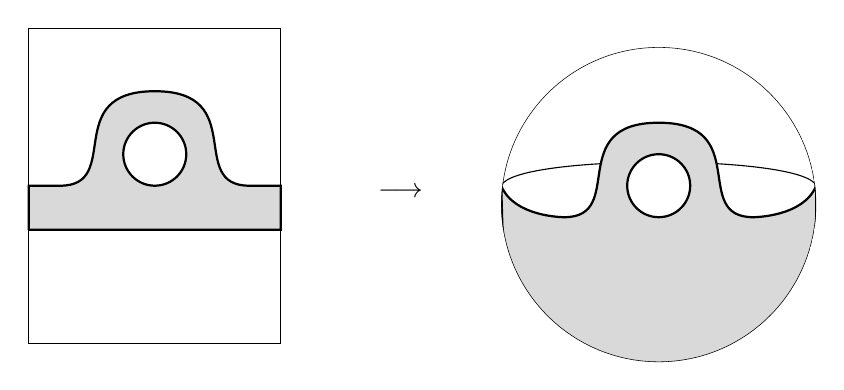
\begin{tikzpicture}[scale=.8]
%\draw[help lines=1,thick] (-5,-3) grid (5,3);
%\foreach \x in {-8,-6,...,8}\draw (\x,0) node{\x};
%\foreach \x/\y in {(0,1)/3,(0,0)/1,(0,-1)/2}
%\foreach \y in {-4,...,4}\draw (0,\y) node{\y};
%
\draw (.9,2.4) node{$\longrightarrow$};
\begin{scope}[xshift=-5cm,yshift=-5mm]
\draw[fill, gray!30!white] (0,2.3)--(0,3)--(.5,3)..controls (1.5,3) and (.5,4.5)..(2,4.5)..controls (3.5,4.5) and (2.5,3)..(3.5,3)--(4,3)--(4,2.3)--(0,2.3);
\draw[thick] (0,2.3)--(0,3)--(.5,3)..controls (1.5,3) and (.5,4.5)..(2,4.5)..controls (3.5,4.5) and (2.5,3)..(3.5,3)--(4,3)--(4,2.3)--(0,2.3);
\draw[white,fill] (2,3.5)circle[radius=5mm];
\draw[thick] (2,3.5)circle[radius=5mm];
\end{scope}
%
\begin{scope}[xshift=-5cm]
\draw (0,0)--(0,5)--(4,5)--(4,0)--cycle;
\end{scope}
%
% the sphere
%
\begin{scope}[xshift=3cm,yshift=-1cm]
\clip (2,3.2) circle[radius=2.5cm];
\draw (-.5,3.5)..controls (-.3,4) and (4.3,4)..(4.5,3.5);

\draw[fill, gray!30!white] (-.4,0)--(-.5,3.5)..controls (-.3,3) and (.5,3)..(.5,3)..controls (1.5,3) and (.5,4.5)..(2,4.5)..controls (3.5,4.5) and (2.5,3)..(3.5,3)..controls (3.5,3) and (4.3,3)..(4.5,3.5)--(4.5,0)--(-.4,0);
\draw[thick] (-.4,0)--(-.5,3.5)..controls (-.3,3) and (.5,3)..(.5,3)..controls (1.5,3) and (.5,4.5)..(2,4.5)..controls (3.5,4.5) and (2.5,3)..(3.5,3)..controls (3.5,3) and (4.3,3)..(4.5,3.5)--(4.5,0)--(-.4,0);

%\draw (-.5,3.5)..controls (-.3,4) and (4.3,4)..(4.5,3.5);
\draw[white,fill] (2,3.5)circle[radius=5mm];
\draw[thick] (2,3.5)circle[radius=5mm];
\draw (2,3.2) circle[radius=2.5cm];

\end{scope}
%
%\coordinate (A) at (0,0);
%\draw[thick,color=blue] (A) ellipse [x radius=2.8cm,y radius=2.1cm];
\end{tikzpicture}
\caption{Tube in square and tube in a sphere, yielding the map $\widetilde{\cT}_{N,k}^p \to \widetilde{\cT}^q_{N,k}$.}
\label{Figure1908}
\end{center}
\end{figure}
%
}

The map $\widetilde{\cT}_{N,k}^p \to \widetilde{\cT}^q_{N,k}$ is not a homotopy equivalence, however by a standard argument the connectivity tends to infinity as you stabilize $N,k \to \infty$ (in the model $\cT_{N,k}^q$ the stabilization is given by direct sum with standard quadratic forms $\|x\|^2-\|y\|^2$, $(x,y) \in \bR^a \times \bR^b$). Indeed, given a tube bundle $W \subset M \times S^{N-1} \to M$ over a compact manifold $M$, so for each $m \in M$ we have a tube $T_m \subset M$. First, since the fiber of the fiber bundle $\partial W \to M$ is diffeomorphic to $S^{k-1} \times S^{N-k-1}$, by increasing $N$ and $k$ we may always find a section $s:M \to \partial W$ of the fibration $\partial W \to M$. Second, as a section of the trivial bundle $M \times S^{N-1}  \to M$ the section $s$ is homotopic through sections to a constant section after increasing $N$ if necessary. By isotopy extension this means we may assume that there is a point, say $x=(0,\ldots,0,1) \in S^{N-1}$ such that $x \in \partial T_m$ for each tube $T_m \subset S^{N-1}$, $m \in M$. Next, note that we may assume that $T_x (\partial T_m) = \bR^{N-2} \times 0 \times 0 \subset \bR^{N-1} \times 0 =  T_xS^{N-1}$ for all $m \in M$. Indeed, again by isotopy extension the only obstruction is linear algebraic and consists of trivializing the outwards pointing normal vector to $\partial T_m$ at $x$, which lives in $[M,S^{N-2}]$ and hence dies if $N$ becomes large enough. At this point it is straightforward to make $W$ standard near an $\varepsilon$-ball about $x \in B \subset S^{N-1}$ and then by a suitably isotopy of $S^{N-1}$ it is then straightforward to make it standard on the entire ball $B \subset S^{N-1}$. If $M$ has boundary this construction all works relative to $\partial M$ and so this proves that the inclusion $\widetilde{\cT}_{N,k}^p\subset \widetilde{\cT}^q_{N,k}$ becomes arbitrarily connected as $N,k \to \infty$.


Therefore we may speak unambiguously of the stable space of tubes $\cT_\infty$, which is the result of stabilizing $N,k\to \infty$, as this stable space is common to both of these models. The monoid $\cT^q=\coprod_{N,k} \cT_{N,k}^q$ consisting of functions of quadratic tube type which we consider in the present article was introduced in \cite{AACK}, and the function space version of $\cT_\infty$ is realized by implementing stabilization of $\cT^q$ as direct sum with suitable standard non-degenerate quadratic forms. The idea of thinking of tubes as codimension zero submanifolds of the sphere had already been introduced in the model of Rognes in \cite{R92}. The advantage of this model is that it is better suited for the monoid (and indeed infinite loopspace) structures at play than the partition model used by Waldhausen. We also have a stable space $\cQ_\infty$ given by stabilizing $N,k \to \infty$ in $\cQ_{N,k}$ in the same way, and the inclusion $\cQ_{k,N} \to \cT_{k,N}$ stabilizes to a map $\cQ_\infty \to \cT_\infty$.
%called the (stable) rigid tube map. Note that there is a homotopy equivalence $\cQ_\infty \to BO$ given by taking the negative eigenspace of a non-degenerate quadratic form. So the rigid tube map is a map 

%For our model $\cT$ as defined in Section \ref{sec: tube bundles} above we have $\cT_\infty$ the colimit of the stabilization maps $\cT \to \cT \to \cdots$ by the standard quadratic form $\|x\|^2-\|y\|^2$ on $\bR^4$. We also denote $\cQ_\infty$ the colimit of the stabilization maps $\cQ \to \cQ \to \cdots$ by the standard quadratic form $\|x\|^2-\|y\|^2$ on $\bR^4$.

In particular, given a fibered function of tube type over $M$ we get an associated map $M \to \cT_\infty$. If the fibered function is of rigid tube type then we get a lift $M \to \cQ_\infty$ through $Q_\infty \to \cT_\infty$. In this case, we may compose this with the equivalence $\cQ_\infty \to BO$ given by taking the negative eigenspace of a non-degenerate quadratic form, and the resulting map $M \to BO$ classifies the stable bundle of the family of quadratic forms $q_m: \bR^N \to \bR$ comprising the fibered function of rigid tube type. % Indeed, it is not hard to show that up to stable equivalence, i.e. direct sum with the standard quadratic forms $\pm x^2$, the map $M \to BO$ classifies fibered functions of rigid tube type. 
Similarly, in the general case of a fibered function of tube type which is not necessarily rigid, one may consider the associated map $M \to \cT_\infty$ and it is shown in \cite{W82} that the homotopy class of this map classifies the fibered function of tube type over $M$ up to stable equivalence.

The map $\cQ_\infty \to \cT_\infty$ called the (stable) {\em rigid tube map}, or more informally we may denote $BO \to \cT_\infty$. It was proved by B\"okstedt that the stable rigid tube map is a rational homotopy equivalence \cite{B82}, a fact which was also proved by the second author using higher Reidemeister torsion in \cite{I02}. For example, for homotopy groups this means that $$\pi_n \cT_\infty \otimes \bQ   \simeq \pi_n BO \otimes \bQ $$ 
which is $\bQ$ if $n$ is of the form $4k$ and is zero otherwise. For $n=4k$, modulo the torsion subgroup, we have a monomorphism of free abelian groups
$$\pi_{4k} BO \xrightarrow{\sim}  (\pi_{4k} \cT_\infty )/\ \text{Tors} $$ 
i.e. up to $\pm 1$ a monomorphism $\bZ \to \bZ$. Let $J_k \in \bZ_{>0}$ be the index of the image. Higher torsion gives an injection $\bZ/J_k\bZ \to \bR/\lambda_k\bZ$ where $\lambda_k = p_k(E)$ for $ E \to S^{4k}$ the generator ok $KO^0(S^{4k})$. So the higher torsion classes are a subtle enough invariant to detect the failure for the rigid tube map $BO \to \cT_\infty$ to be surjective on homotopy groups modulo the  torsion subgroup $\text{Tors} (  \pi_{4k} \cT_\infty )$.
 %However, it is not a homotopy equivalence, which as we will see is the basis for the nontriviality of the Legendrian invariant we will construct using functions of tube type. 

Following \cite{W82}  consider  $\cH_\infty$, the  {\em stable space of h-cobordisms of a point}, denoted $\cH_\infty$, which is a classifying space for fiber bundles $V \to M$ whose fiber is an h-cobordism of a disk $D^k$, i.e. diffeomorphic to $D^k \times [0,1]$ with a fixed trivialization of the lower boundary $D^k \times \{0 \}$, up to stable equivalence. Waldhausen defined a map $\cH_\infty \to \cT_\infty$ given by stacking an h-cobordism of a disk on top of a standard tube, see Figure \ref{Figure1903}.

{
%
\begin{figure}[htbp]
\begin{center}
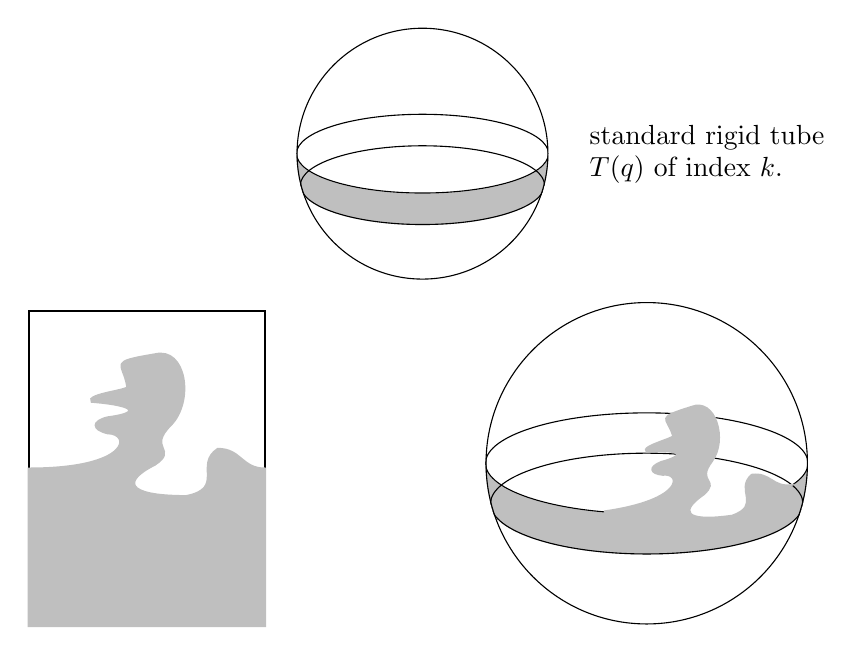
\begin{tikzpicture}%[scale=1.4]
%\draw[help lines=1,thin] (-5,-3) grid (5,6);
%\foreach \x in {-8,-6,...,8}\draw (\x,0) node{\x};
%\foreach \x/\y in {(0,1)/3,(0,0)/1,(0,-1)/2}
%\foreach \y in {-4,...,4}\draw (0,\y) node{\y};
%\draw (4,0) circle[radius=2cm];

\begin{scope}[xshift=1cm,yshift=.25cm]% h-cobordism
\draw[thick] (-5,1.75)--(-5,-2.25)--(-2,-2.25)--(-2,1.75)--cycle;
\draw[thick,fill,gray!50!white] (-5,-2.25)--(-5,-.25)..controls (-3.7,-.25) and (-3.7,0.2)..(-4,0.2)..controls (-4.2,.25) and (-4.2,.35)..(-4,.4)..controls (-3.6,.45) and (-3.6,.55)..(-4.2,.6)..controls(-4.3,.7) and (-3.65,.75)..(-3.75,.8)..controls (-3.8,1.1) and(-4,1.1)..(-3.4,1.2)..controls (-3,1.3) and (-2.9,.6).. (-3.2,.3)..controls (-3.5,0) and (-3.1,0)..(-3.4,-.2)..controls (-3.8,-.4) and (-3.8,-.6)..(-3,-.6)..controls (-2.5,-.5) and (-2.9,-.2)..(-2.6,0)..controls (-2.3,0) and (-2.3,-.25)..(-2,-.25)--(-2,-2.25)--cycle;%--(-2,-.25);
\end{scope}

\begin{scope}% small sphere
\clip (1,4) circle[radius=1.6cm];
\draw[fill,gray!50!white] (1,3.6) ellipse[x radius=1.55cm,y radius=.5cm];
\draw[fill,gray!50!white] (1,3.8) ellipse[x radius=1.7cm,y radius=.5cm];
\draw[fill,white] (1,4) ellipse[x radius=1.6cm,y radius=.5cm];
\draw(1,4) ellipse[x radius=1.6cm,y radius=.5cm];
\draw (1,3.6) ellipse[x radius=1.55cm,y radius=.5cm];
\draw[thick] (1,4) circle[radius=1.6cm];
\end{scope}

\begin{scope}[rotate=8, scale=.8,yshift=-1.5cm] % big sphere with h-cobordism
\begin{scope}[xshift=2.3cm,yshift=-5.2cm,rotate=-8,scale=1.6]% big sphere
\clip (1,4) circle[radius=1.6cm];
\draw[fill,gray!50!white] (1,3.6) ellipse[x radius=1.55cm,y radius=.5cm];
\draw[fill,gray!50!white] (1,3.8) ellipse[x radius=1.7cm,y radius=.5cm];
\draw[fill,white] (1,4) ellipse[x radius=1.6cm,y radius=.5cm];
\draw(1,4) ellipse[x radius=1.6cm,y radius=.5cm];
\draw (1,3.6) ellipse[x radius=1.55cm,y radius=.5cm];
\draw[thick] (1,4) circle[radius=1.6cm];
\end{scope}
%
\begin{scope}[xshift=9cm,yshift=.5cm]% shifted h-cobordism
\clip (-3.2,-.5) circle[radius=.6cm];
\draw[fill,white] (-5,-.25)..controls (-3.7,-.25) and (-3.7,0.2)..(-4,0.2)..controls (-4.2,.25) and (-4.2,.35)..(-4,.4)..controls (-3.6,.45) and (-3.6,.55)..(-4.2,.6)..controls(-4.3,.7) and (-3.65,.75)..(-3.75,.8)..controls (-3.8,1.1) and(-4,1.1)..(-3.4,1.2)..controls (-3,1.3) and (-2.9,.6).. (-3.2,.3)..controls (-3.5,0) and (-3.1,0)..(-3.4,-.2)..controls (-3.8,-.4) and (-3.8,-.6)..(-3,-.6)..controls (-2.5,-.5) and (-2.9,-.2)..(-2.6,0)..controls (-2.3,0) and (-2.3,-.25)..(-2,-.25)..controls (-3,-.4) and (-4,-.4)..(-5,-.25);%--(-2,-.25);
\end{scope}
\begin{scope}[xshift=9cm,yshift=.5cm]% shifted h-cobordism
\draw[thick,fill,gray!50!white] (-5,-.25)..controls (-3.7,-.25) and (-3.7,0.2)..(-4,0.2)..controls (-4.2,.25) and (-4.2,.35)..(-4,.4)..controls (-3.6,.45) and (-3.6,.55)..(-4.2,.6)..controls(-4.3,.7) and (-3.65,.75)..(-3.75,.8)..controls (-3.8,1.1) and(-4,1.1)..(-3.4,1.2)..controls (-3,1.3) and (-2.9,.6).. (-3.2,.3)..controls (-3.5,0) and (-3.1,0)..(-3.4,-.2)..controls (-3.8,-.4) and (-3.8,-.6)..(-3,-.6)..controls (-2.5,-.5) and (-2.9,-.2)..(-2.6,0)..controls (-2.3,0) and (-2.3,-.25)..(-2,-.25)..controls (-3,-.85) and (-4,-.85)..(-5,-.25);%--(-2,-.25);
\end{scope} % end of shifted h-cobordism
\end{scope} % end of big sphere with shifted h-cobordism

\begin{scope}[xshift=3cm,yshift=4cm]
\draw (0,.2) node[right]{standard rigid tube};
\draw (0,-.2) node[right]{$T(q)$ of index $k$.};
\end{scope}

%\coordinate (A) at (0,0);
%\draw[thick,color=blue] (A) ellipse [x radius=2.8cm,y radius=2.1cm];
\end{tikzpicture}
\caption{On the left is an $h$-cobordism of a disk representing an element of $\cH_\infty$ as a partition of $[-1,1]^{n-1}\times[0,1]$. On the right is the tube of index $k$ obtained by pasting the $h$-cobordism into $S^{n}$ on top of the standard rigid tube of index $k$ shown in the middle. This yields a map $\cH_\infty \to \cT_\infty$.}
\label{Figure1903}
\end{center}
\end{figure}
%
}



Consider also the forgetful map $\cT_\infty \to \cT_\infty^{\text{TOP}}$ in which $ \cT_\infty^{\text{TOP}}$ is the stable space of tubes in the topological category. It was shown by Waldhausen in \cite{W82} that $\cT_\infty^{\text{TOP}} \simeq BG$ for $BG$ the classifying space for spherical fibrations, i.e. $G=\lim_N G_N$ for $G_N$ the space of maps $S^N \to S^N$ of degree $\pm 1$. 



\begin{theorem}[\cite{W82}]\label{thm: wald fib} $\cH_\infty \to \cT_\infty \to BG$ is a fibration sequence. \end{theorem}

Consider the map $BG \to B (\bZ/2)$ induced by the degree map $G \to \bZ/2$. To a tube bundle $W \to M$, with stable equivalence class classified by a map $M \to \cT_\infty$, is associated a map $M \to B (\bZ/2)$. This map is nullhomotopic precisely when $W$ is orientable. Higher torsion is not defined for non-orientable tube bundles, i.e. higher torsion is a characteristic class coming from the cohomology of the fiber of the map $\cT_\infty \to B(\bZ/2)$. Note that the composition $\cH_\infty \to \cT_\infty \to BG \to B(\bZ/2)$ is trivial and so tube bundles which come from h-cobordism bundles are automatically orientable. 

We also note that the higher torsion of a tube bundle changes sign under stabilization by the standard form $x^2-y^2$ on $\bR^2$ since the index $k$ changes parity. For this reason it is better to assume that all ambient dimensions are even and always stabilize by a non-degenerate form of even index in an even dimensional ambient space, which always leaves torsion unchanged. With this modification of $\cT_\infty$ (and similarly for $\cH_\infty$ and $\cQ_\infty$), any homotopy class of map $M \to \cT_\infty$ such that the composite $M \to B(\bZ/2)$ is null determines higher torsion classes in $M$. In particular any homotopy class of map $M \to \cH_\infty$ determines higher torsion classes  in $M$. The following observation, which will be our source of examples of Legendrians with non-trivial tube torsion in Section \ref{sec: nontriv} below. 

\begin{proposition} If $V \to M$ is a bundle of h-cobordisms of a disk classified by $M \to \cH_\infty$ and $W \to M$ is the stable tube bundle classified by the composition $M \to \cH_\infty \to  \cT_\infty$, then there holds $\tau_k(V)=\tau_k(W)$.  \end{proposition}

\begin{proof} The tube bundle $W$ is obtained by gluing $V$ to the trivial tube bundle $M \times T$ for $T$ the standard tube. By Theorem \ref{thm: framed function} we may choose a function $f:V \to \bR$ with moderate singularities which is standard near the top and bottom of each h-cobordism, i.e. such that on each fiber $D^m \times [0,1]$ the restriction of $f$ is standard near top and bottom. We may glue such a function $f$ to the standard quadratic form $q:M \times T \to \bR$ on the trivial tube bundle $M \times T$  to obtain a function with moderate singularities $h:W \to \bR$ whose paramerized Morse theory consists of the union of that of $f$ and (the constant family) $q$. The proof is then completed by applying the framing principle Theorem \ref{thm: framing} to compute $\tau_k(W)$ using the function $h:W \to \bR$ on the glued up tube bundle and to compute $\tau_k(V)$ using the function $f:V \to \bR$ on the original bundle of h-cobordisms. The two computations yields the same expression because the extra contribution from $q$ to both the parametrized Morse complex and to the stable bundle is trivial.   \end{proof}


\begin{remark} Given a Legendrian $\Lambda \subset J^1M$, consider the subset $\cT(\Lambda) \subset [M,\cT_\infty]$ consisting of homotopy classes of maps classifying a stable tube bundle on which $\Lambda$ admits a generating function. The homotopy lifting theorem for generating functions implies that $\cT(\Lambda)$ is a Legendrian isotopy invariant. The tube torsion classes that we consider in the present article are a cohomological shadow of the a priori finer invariant $\cT(\Lambda)$.  \end{remark}%Indeed, the  higher torsion of an orientable tube bundle classified by  $M \to \cT_\infty$ is the pullback of a universal class in $H^*(\cT_\infty^{or})$ by a lift $M \to \cT_\infty^{or}$ to the fiber of the sequence $\cT_\infty^{or} \to \cT_\infty \to B(\bZ/2)$, i.e. higher torsion is a {\em characteristic class} of orientable tube bundles.



\begin{remark}
 By the stable parametrized stable h-cobordism theorem of Waldhausen $\cH_\infty$ is closely related to $K(\mathbf{S})$, the algebraic K-theory of the sphere spectrum, i.e. $A(\ast)$, the Waldhausen K-theory of a point. Hence by Theorem \ref{thm: wald fib} the stable space of tubes $\cT_\infty$ is also closely related to $A(\ast)$. As noted in the remark after Proposition 3.1 of \cite{W82}, there is a homotopy cartesian square
$$
\begin{tikzcd} \cT_\infty \ar[r] \ar[d] & BG\ar[d] \\
 \Omega^\infty S^\infty \ar[r]& A( \ast)
\end{tikzcd} $$
\end{remark}

\begin{remark}
There is another important positive integer $I_k \in \bZ_{>0}$, which is closely related to $J_k$. Waldhausen in \cite{W82} more generally discussed a homotopy commutative square where the columns are fibration sequences
$$
\begin{tikzcd}  G/ O\ar[r] \ar[d] & \cH_\infty \ar[d] \\
BO \ar[r] \ar[d] & \cT_\infty  \ar[d]\\
BG \ar[r,"="] & BG 
\end{tikzcd} $$
The vertical column is the $J$-map fibration $G/O \to BO \to BG$ and the top row is the {\em Hatcher-Waldhausen map} $G/O \to \cH_\infty$, which is a rational equivalence by that same theorem of B\"okstedt  \cite{B82}. For $n=4k$, modulo the torsion subgroups, we have a monomorphism of free abelian groups
$$(\pi_{4k} G/O) / \text{Tors} \xrightarrow{\sim} (\pi_{4k} \cH_\infty) / \text{Tors} $$ 
i.e.  up to $\pm 1$ a monomorphism $\bZ \to \bZ$. Let $I_k \in \bZ_{>0}$ be the index of the image. The integers $I_k$ and $J_k$ are thus closely related by the J-homomorphism. From private communication from S. Kupers we understand that in principle a careful comparison of the literature, including a careful comparison of conventions for regulators and for higher torsion classes, could lead to concrete information on the integers $I_k$ and $J_k$. 

The integer $I_k$ is also closely related to the mysterious finite homotopy group $\pi_{4k}\cM_\infty$ of the space $\cM_\infty$ considered by Kragh in \cite{Kra18}, who proved that the Hatcher map extends to a fibration sequence $\cM_\infty \to G/O \to \cH_\infty$ where $\cM_\infty$ is roughly speaking the stable space of functions $\bR^{2N} \to \bR$ equal to the standard quadratic form $\|x\|^2-\|y\|^2$ at infinity and which have a unique and non-degenerate critical point. The space $\cM_\infty$ is related to generating functions for {\em Long nearby Lagrangian knots} in $T^*\bR^k$.  Indeed, in \cite{Kra18} it is shown that if $L \subset T^*\bR^k$ is an exact Lagrangian submanifold agreeing with the zero section $\bR^k \subset T^*\bR^k$ outside of a compact set, then $L$ admits a generating function $f:\bR^k \times \bR^{2N} \to \bR$ which is {\em standard-quadratic} at infinity and hence by restricting to a large sphere in $\bR^k$ one obtains an element of $\pi_{k-1} \cM_\infty$ which is closely related to the torsion invariants considered in the present article. The Hatcher-Waldhausen map $G/O \to \cH_\infty$ was shown to be an infinite loop map by Rognes in \cite{R92}.
\end{remark}

\subsection{Legendrians with nontrivial tube torsion}\label{sec: nontriv}

We are now ready to establish for general $M$ the existence of Legendrians $\Lambda \subset J^1M$ such that the projection $\Lambda \to M$ is homotopic to a diffeomorphism and which have nontrivial tube torsion. In particular this shows that the vanishing of the tube torsion of nearby Lagrangians $L \subset T^*M$ predicted by the nearby Lagrangian conjecture cannot rely solely on the fact that the projection $L \to M$ is a homotopy equivalence (or even from a conjectural expectation that the projection $L \to M$ is homotopic to a diffeomorphism, which is not known).

Recall that given a bundle of h-cobordisms of a disk $V \to M$, the stable equivalence class of the bundle is classified by the homotopy class of a map $M \to \cH_\infty$, see Section \ref{sec: SpaceOfTubes}. By the fibration sequence $\cH_\infty \to \cT_\infty \to BG$ of Waldhausen \cite{W82} there is an associated tube bundle $W \to M$ which geometrically is obtained by attaching $V$ onto a trivial bundle of tubes $M \times T \to M$. 

We recall that Theorem \ref{thm: existence of example} states that given a bundle of h-cobordisms of a disk $V  \to M$, there exists a Legendrian $\Lambda \subset J^1M$ whose projection $\Lambda \to M$ is homotopic to a diffeomorphism and which admits a generating function on the tube bundle $W \to M$ obtained from $V$ via the map $\cH_\infty \to \cT_\infty$. 

%\begin{definition}
%Given $g:\bR^N \to \bR$ a function of quadratic tube type, $\nabla g:\bR^N \to \bR^N$ is homogeneous of degree 1 and has degree $\pm 1$, hence may be viewed as a map $S^N \to S^N$. This gives a map $\cT_{k,N} \to G_N$ for $G_N$ the space of self-homotopy equivalences of $S^N$ which stabilizes to a map $D: \cT_\infty \to G$ called the {\em Waldhausen derivative}. 
%\end{definition}

\begin{proof}[Proof of Theorem \ref{thm: existence of example}]
We may apply Theorem \ref{thm: wrinkling} to the bundle of $h$-cobordisms $V$, where we take $A$ to consist of $\partial V$ and $g: Op(A) \to \bR$ to be a function on $Op(A)$ without critical points for which the two components of $\partial V$ (corresponding to the boundary components $D^k \times \{0\}$ and $D^k \times \{1\}$  of the fiber $D^k \times [0,1]$) are regular level sets of $g$. To verify the hypothesis of Theorem \ref{thm: wrinkling} that $d_vg$ extends to a non-vanishing section of $\text{Vert}^*$ we may argue as in Proposition 2.5 in \cite{EM00}, though note the attribution there to earlier work of Douady and Laudenbach, as well as to the second author's PhD thesis. 

After applying Theorem \ref{thm: wrinkling} we conclude that there exists a fibered wrinkled function $h:V \to \bR$ such that the lower boundary $\partial_0 V$ is a regular level set for $h$. Hence $h$ can be stitched up with a standard function on the trivial tube bundle $q: M \times T \to \bR$ to obtain a function with moderate singularities $h \# q :W \to \bR$ whose fiberwise critical set $\Sigma_f$ is the disjoint union of $\Sigma_h$ and $\Sigma_q$, where $\Sigma_q \to M$ is a diffeomorphism. Hence $h \# q$ generates a Legendrian $\Lambda \subset J^1M$ which is the disjoint union of finitely many Legendrian spheres $S_i \subset J^1M$, each diffeomorphic to the standard sphere and whose projection $S_i \to M$ is nullhomotopic, and the zero section $M \subset J^1M$, see Figure \ref{Figure1906a}. Note that each $S_i$ may sit as a complicated Legendrian knot in $J^1M$, and the union of the $S_i$ as a complicated Legendrian link, but each front $S_i \to J^1M$ has only cusp singularities (along an equator $C_i \subset S_i$). 

Next, we note using Proposition 3.21 of \cite{ACGK} one may construct a fibered function of tube type $f:M \times \bR^N \to \bR$ such that $W=T(f)$ and which generates the same Legendrian $\Lambda$ (the statement of Proposition 3.21 only states it up to Legendrian isotopy but one may appeal to the homotopy lifting property after further stabilization if necessary). After a further Legendrian isotopy of $\Lambda$, (which againis covered by a homotopy of functions $f$ having the same properties after stabilization if necessary), we may arrange it so the Legendrian $\Lambda$ has cusps of any Maslov index (spin a Reidemeister I move and use this to make pagodas of increasing and decreasing Maslov index at any given point of the graphical component of $\Lambda$, see Figure \ref{Figure1906b}). We can then use a surgery of corank 1 singularities to surger the spheres $S_i$ into the Legendrian $\Lambda$ via connect sum, again covering the deformation by a homotopy of functions $f$ having the same properties, except now the components $S_i$ have been absorbed into the graphical component of the Legendrian, see Figure \ref{Figure1907}. Thus the diffeomorphism type of $\Lambda$ is equal to the connect sum of $M$ with finitely many standard spheres, so the final Legendrian $\Lambda$ is diffeomorphic to $M$ and moreover the projection $M \to \Lambda$ is homotopic to a diffeomorphism.   \end{proof}

{
%
\begin{figure}[htbp]
\begin{center}
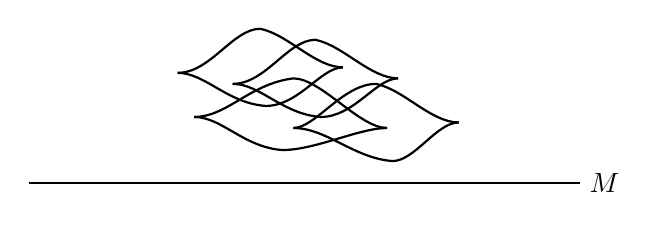
\begin{tikzpicture}[scale=.7]
%\draw[help lines=1,thin] (-5,-3) grid (5,3);
%\foreach \x in {-8,-6,...,8}\draw (\x,0) node{\x};
%\foreach \x/\y in {(0,1)/3,(0,0)/1,(0,-1)/2}
%\foreach \y in {-4,...,4}\draw (0,\y) node{\y};

{
\begin{scope}[yshift=5cm]%top figure with 4 wrinkles
\begin{scope}
\draw[thick] (-5,0)--(5,0);
\draw (5,0) node[right]{$M$};
\end{scope}
\begin{scope}[yshift=2cm,xshift=-2.3cm] % top left wrinkle
\draw[thick] (0,0)..controls (.6,0) and (1,.8)..(1.5,.8)..controls (2,.7) and (2.5,0.1)..(3,.1);
\draw[thick](0,0)..controls (.5,0)and(.9,-.55)..(1.6,-.6)..controls (2.2,-.6) and (2.6,.1)..(3,.1);
\end{scope}
%
\begin{scope}[yshift=1.8cm,xshift=-1.3cm] % top right wrinkle
\draw[thick] (0,0)..controls (.6,0) and (1,.8)..(1.5,.8)..controls (2,.7) and (2.5,0.1)..(3,.1);
\draw[thick](0,0)..controls (.5,0)and(.9,-.55)..(1.6,-.6)..controls (2.2,-.6) and (2.6,.1)..(3,.1);
\end{scope}
%
\begin{scope}[yshift=1cm,xshift=-.2cm] % bottom right wrinkle
\draw[thick] (0,0)..controls (.4,0) and (.9,.8)..(1.5,.8)..controls (2,.7) and (2.5,0.1)..(3,.1);
\draw[thick](0,0)..controls (.6,0)and(1.1,-.55)..(1.8,-.6)..controls (2.2,-.6) and (2.6,.1)..(3,.1);
\end{scope}
%
\begin{scope}[yshift=1.2cm,xshift=-2cm] % bottom left wrinkle
\draw[thick] (0,0)..controls (.6,0) and (1,.6)..(1.8,.7)..controls (2.3,.7) and (3,-0.2)..(3.5,-.2);
\draw[thick](0,0)..controls (.5,0)and(.9,-.55)..(1.6,-.6)..controls (2.2,-.6) and (3,-.2)..(3.5,-.2);
\end{scope}
\end{scope}
}

\end{tikzpicture}
\caption{Proof of Theorem \ref{thm: existence of example}, Step 1: Construct a function on the tube bundle $W$ whose Cerf diagram has a copy of the zero section and a bunch of wrinkles.}
\label{Figure1906a}
\end{center}
\end{figure}
%
}


{
%
\begin{figure}[htbp]
\begin{center}
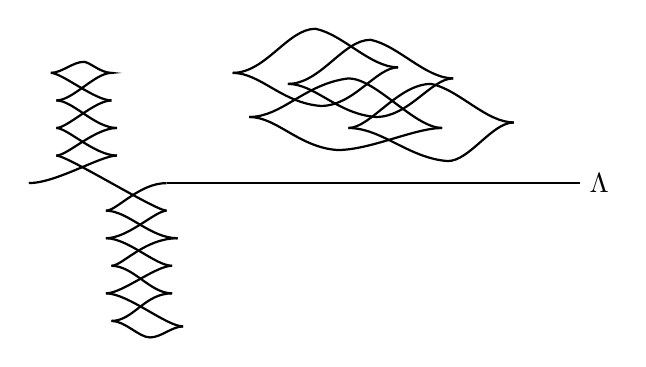
\begin{tikzpicture}[scale=.7]
%\draw[help lines=1,thin] (-5,-3) grid (5,3);
%\foreach \x in {-8,-6,...,8}\draw (\x,0) node{\x};
%\foreach \x/\y in {(0,1)/3,(0,0)/1,(0,-1)/2}
%\foreach \y in {-4,...,4}\draw (0,\y) node{\y};

{
\begin{scope}[xshift=1cm]%bottom figure with 4 wrinkles and 2 zigzags
\begin{scope}% bottom zig-zag
\draw[thick] (-3.5,0)--(4,0);
\draw (4,0) node[right]{$\Lambda$};
\draw[thick] (-3.5,0)..controls (-4,0) and (-4.4,-.5)..(-4.6,-.5);
\draw[thick] (-4.6,-.5)..controls (-4.2,-.5) and (-3.8,-1)..(-3.3,-1);
\draw[thick] (-3.3,-1)..controls (-3.9,-1) and (-4.3,-1.5)..(-4.5,-1.5);
\draw[thick] (-4.5,-1.5)..controls (-4.1,-1.5) and (-3.8,-2)..(-3.4,-2);
\draw[thick] (-3.4,-2)..controls (-3.9,-2) and (-4.1,-2.5)..(-4.5,-2.5);
\draw[thick] (-4.5,-2.5)..controls (-4.25,-2.5) and (-4,-2.8)..(-3.8,-2.8)..controls (-3.6,-2.8) and (-3.4,-2.6)..(-3.2,-2.6);
\draw[thick](-3.2,-2.6)..controls (-3.5,-2.6) and (-4.2,-2)..(-4.6,-2);
\draw[thick] (-4.6,-2)..controls (-4.3,-2) and (-3.7,-1.5)..(-3.4,-1.5);
\draw[thick] (-3.4,-1.5)..controls (-3.7,-1.5) and (-4.2,-1)..(-4.6,-1);
\draw[thick] (-4.6,-1)..controls (-4.2,-1) and (-3.7,-.5)..(-3.5,-.5);
%\draw (5,0) node[right]{$M$};
\end{scope}
\begin{scope}% top zig-zag
\draw[thick] (-3.5,-.5)..controls (-3.7,-.5) and (-5.3,.5)..(-5.5,.5);
\draw[thick] (-5.5,.5)..controls (-5.3,.5) and (-4.8,1)..(-4.4,1);
\draw[thick] (-4.4,1)..controls (-4.8,1) and (-5.2,1.5)..(-5.5,1.5);
\draw[thick] (-5.5,1.5)..controls (-5.2,1.5) and (-4.8,2)..(-4.5,2)..controls (-4.7,2) and (-4.9,2.2)..(-5,2.2)..controls (-5.2,2.2) and (-5.4,2)..(-5.6,2);
\draw[thick] (-5.6,2)..controls (-5.4,2) and (-4.8,1.5)..(-4.5,1.5);
\draw[thick] (-4.5,1.5)..controls (-4.8,1.5) and (-5.3,1)..(-5.5,1);
\draw[thick] (-5.5,1)..controls (-5.3,1) and (-4.8,.5)..(-4.4,.5);
\draw[thick] (-4.4,.5)..controls (-4.7,.5) and (-5.5,0)..(-6,0);%--(-7,0);
\end{scope}
%
\begin{scope}[yshift=2cm,xshift=-2.3cm] % top left wrinkle
\draw[thick] (0,0)..controls (.6,0) and (1,.8)..(1.5,.8)..controls (2,.7) and (2.5,0.1)..(3,.1);
\draw[thick](0,0)..controls (.5,0)and(.9,-.55)..(1.6,-.6)..controls (2.2,-.6) and (2.6,.1)..(3,.1);
\end{scope}
%
\begin{scope}[yshift=1.8cm,xshift=-1.3cm] % top right wrinkle
\draw[thick] (0,0)..controls (.6,0) and (1,.8)..(1.5,.8)..controls (2,.7) and (2.5,0.1)..(3,.1);
\draw[thick](0,0)..controls (.5,0)and(.9,-.55)..(1.6,-.6)..controls (2.2,-.6) and (2.6,.1)..(3,.1);
\end{scope}
%
\begin{scope}[yshift=1cm,xshift=-.2cm] % bottom right wrinkle
\draw[thick] (0,0)..controls (.4,0) and (.9,.8)..(1.5,.8)..controls (2,.7) and (2.5,0.1)..(3,.1);
\draw[thick](0,0)..controls (.6,0)and(1.1,-.55)..(1.8,-.6)..controls (2.2,-.6) and (2.6,.1)..(3,.1);
\end{scope}
%
\begin{scope}[yshift=1.2cm,xshift=-2cm] % bottom left wrinkle
\draw[thick] (0,0)..controls (.6,0) and (1,.6)..(1.8,.7)..controls (2.3,.7) and (3,-0.2)..(3.5,-.2);
\draw[thick](0,0)..controls (.5,0)and(.9,-.55)..(1.6,-.6)..controls (2.2,-.6) and (3,-.2)..(3.5,-.2);
\end{scope}
\end{scope}
}
%\coordinate (A) at (0,0);
%\draw[thick,color=blue] (A) ellipse [x radius=2.8cm,y radius=2.1cm];
\end{tikzpicture}
\caption{Proof of Theorem \ref{thm: existence of example}, Step 2: Obtain cusps of any Maslov index on the copy of the zero section by spinning Reidemeister I moves.}
\label{Figure1906b}
\end{center}
\end{figure}
%
}

{
%
\begin{figure}[htbp]
\begin{center}
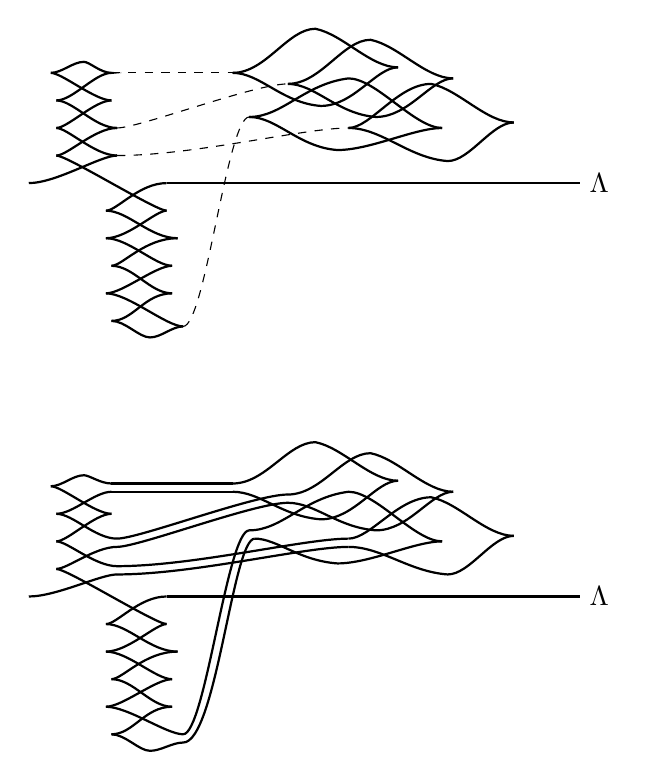
\begin{tikzpicture}[scale=.7]
%\draw[help lines=1,thin] (-5,-3) grid (5,3);
%\foreach \x in {-8,-6,...,8}\draw (\x,0) node{\x};
%\foreach \x/\y in {(0,1)/3,(0,0)/1,(0,-1)/2}
%\foreach \y in {-4,...,4}\draw (0,\y) node{\y};
%\coordinate (A) at (0,0);
{
\begin{scope}[yshift=7.5cm]%bottom figure with 4 wrinkles and 2 zigzags
\begin{scope}% bottom zig-zag
\draw[thick] (-3.5,0)--(4,0);
\draw (4,0) node[right]{$\Lambda$};
\draw[thick] (-3.5,0)..controls (-4,0) and (-4.4,-.5)..(-4.6,-.5);
\draw[thick] (-4.6,-.5)..controls (-4.2,-.5) and (-3.8,-1)..(-3.3,-1);
\draw[thick] (-3.3,-1)..controls (-3.9,-1) and (-4.3,-1.5)..(-4.5,-1.5);
\draw[thick] (-4.5,-1.5)..controls (-4.1,-1.5) and (-3.8,-2)..(-3.4,-2);
\draw[thick] (-3.4,-2)..controls (-3.9,-2) and (-4.1,-2.5)..(-4.5,-2.5);
\draw[thick] (-4.5,-2.5)..controls (-4.25,-2.5) and (-4,-2.8)..(-3.8,-2.8)..controls (-3.6,-2.8) and (-3.4,-2.6)..(-3.2,-2.6);
\draw[thick](-3.2,-2.6)..controls (-3.5,-2.6) and (-4.2,-2)..(-4.6,-2);
\draw[thick] (-4.6,-2)..controls (-4.3,-2) and (-3.7,-1.5)..(-3.4,-1.5);
\draw[thick] (-3.4,-1.5)..controls (-3.7,-1.5) and (-4.2,-1)..(-4.6,-1);
\draw[thick] (-4.6,-1)..controls (-4.2,-1) and (-3.7,-.5)..(-3.5,-.5);
%\draw (5,0) node[right]{$M$};
\end{scope}
\begin{scope}% top zig-zag
\draw[thick] (-3.5,-.5)..controls (-3.7,-.5) and (-5.3,.5)..(-5.5,.5);
\draw[thick] (-5.5,.5)..controls (-5.3,.5) and (-4.8,1)..(-4.4,1);
\draw[thick] (-4.4,1)..controls (-4.8,1) and (-5.2,1.5)..(-5.5,1.5);
\draw[thick] (-5.5,1.5)..controls (-5.2,1.5) and (-4.8,2)..(-4.5,2)..controls (-4.7,2) and (-4.9,2.2)..(-5,2.2)..controls (-5.2,2.2) and (-5.4,2)..(-5.6,2);
\draw[thick] (-5.6,2)..controls (-5.4,2) and (-4.8,1.5)..(-4.5,1.5);
\draw[thick] (-4.5,1.5)..controls (-4.8,1.5) and (-5.3,1)..(-5.5,1);
\draw[thick] (-5.5,1)..controls (-5.3,1) and (-4.8,.5)..(-4.4,.5);
\draw[thick] (-4.4,.5)..controls (-4.7,.5) and (-5.5,0)..(-6,0);%--(-7,0);
\end{scope}
%
\begin{scope}[yshift=2cm,xshift=-2.3cm] % top left wrinkle
\draw[thick] (0,0)..controls (.6,0) and (1,.8)..(1.5,.8)..controls (2,.7) and (2.5,0.1)..(3,.1);
\draw[thick](0,0)..controls (.5,0)and(.9,-.55)..(1.6,-.6)..controls (2.2,-.6) and (2.6,.1)..(3,.1);
\end{scope}
%
\begin{scope}[yshift=1.8cm,xshift=-1.3cm] % top right wrinkle
\draw[thick] (0,0)..controls (.6,0) and (1,.8)..(1.5,.8)..controls (2,.7) and (2.5,0.1)..(3,.1);
\draw[thick](0,0)..controls (.5,0)and(.9,-.55)..(1.6,-.6)..controls (2.2,-.6) and (2.6,.1)..(3,.1);
\end{scope}
%
\begin{scope}[yshift=1cm,xshift=-.2cm] % bottom right wrinkle
\draw[thick] (0,0)..controls (.4,0) and (.9,.8)..(1.5,.8)..controls (2,.7) and (2.5,0.1)..(3,.1);
\draw[thick](0,0)..controls (.6,0)and(1.1,-.55)..(1.8,-.6)..controls (2.2,-.6) and (2.6,.1)..(3,.1);
\end{scope}
%
\begin{scope}[yshift=1.2cm,xshift=-2cm] % bottom left wrinkle
\draw[thick] (0,0)..controls (.6,0) and (1,.6)..(1.8,.7)..controls (2.3,.7) and (3,-0.2)..(3.5,-.2);
\draw[thick](0,0)..controls (.5,0)and(.9,-.55)..(1.6,-.6)..controls (2.2,-.6) and (3,-.2)..(3.5,-.2);
\end{scope}
\draw[dashed] (-3.2,-2.6)..controls (-2.8,-2.6) and (-2.4,1.2)..(-2,1.2);
\draw[dashed] (-4.4,.5)..controls (-3,.5)and (-1,1)..(-.2,1);
\draw[dashed] (-4.5,2)--(-2.3,2);
\draw[dashed] (-4.4,1)..controls (-4,1)and(-1.9,1.8)..(-1.3,1.8);
\end{scope}
}

{
\begin{scope}%[yshift=8cm]%bottom figure with 4 wrinkles and 2 zigzags
\begin{scope}% bottom zig-zag
\draw[thick] (-3.5,0)--(4,0);
\draw (4,0) node[right]{$\Lambda$};
\draw[thick] (-3.5,0)..controls (-4,0) and (-4.4,-.5)..(-4.6,-.5);
\draw[thick] (-4.6,-.5)..controls (-4.2,-.5) and (-3.8,-1)..(-3.3,-1);
\draw[thick] (-3.3,-1)..controls (-3.9,-1) and (-4.3,-1.5)..(-4.5,-1.5);
\draw[thick] (-4.5,-1.5)..controls (-4.1,-1.5) and (-3.8,-2)..(-3.4,-2);
\draw[thick] (-3.4,-2)..controls (-3.9,-2) and (-4.1,-2.5)..(-4.5,-2.5);
\draw[thick] (-4.5,-2.5)..controls (-4.25,-2.5) and (-4,-2.8)..(-3.8,-2.8)..controls (-3.6,-2.8) and (-3.4,-2.65)..(-3.2,-2.65);
\draw[thick](-3.2,-2.5)..controls (-3.5,-2.5) and (-4.2,-2)..(-4.6,-2);
\draw[thick] (-4.6,-2)..controls (-4.3,-2) and (-3.7,-1.5)..(-3.4,-1.5);
\draw[thick] (-3.4,-1.5)..controls (-3.7,-1.5) and (-4.2,-1)..(-4.6,-1);
\draw[thick] (-4.6,-1)..controls (-4.2,-1) and (-3.7,-.5)..(-3.5,-.5);
%\draw (5,0) node[right]{$M$};
\end{scope}
\begin{scope}% top zig-zag
\draw[thick] (-3.5,-.5)..controls (-3.7,-.5) and (-5.3,.5)..(-5.5,.5);
\draw[thick] (-5.5,.5)..controls (-5.3,.5) and (-4.8,.9)..(-4.4,.9);
\draw[thick] (-4.4,1.05)..controls (-4.8,1.05) and (-5.2,1.5)..(-5.5,1.5);
\draw[thick] (-5.5,1.5)..controls (-5.2,1.5) and (-4.8,1.9)..(-4.5,1.9);
\draw[thick] (-4.5,2.05)..controls (-4.7,2.05) and (-4.9,2.2)..(-5,2.2)..controls (-5.2,2.2) and (-5.4,2)..(-5.6,2);
\draw[thick] (-5.6,2)..controls (-5.4,2) and (-4.8,1.5)..(-4.5,1.5);
\draw[thick] (-4.5,1.5)..controls (-4.8,1.5) and (-5.3,1)..(-5.5,1);
\draw[thick] (-5.5,1)..controls (-5.3,1) and (-4.8,.55)..(-4.4,.55);
\draw[thick] (-4.4,.4)..controls (-4.7,.4) and (-5.5,0)..(-6,0);%--(-7,0);
\end{scope}
%
\begin{scope}[yshift=2cm,xshift=-2.3cm] % top left wrinkle
\draw[thick] (0,0.05)..controls (.6,0.05) and (1,.8)..(1.5,.8)..controls (2,.7) and (2.5,0.1)..(3,.1);
\draw[thick](0,-.1)..controls (.5,-.1)and(.9,-.55)..(1.6,-.6)..controls (2.2,-.6) and (2.6,.1)..(3,.1);
\end{scope}
%
\begin{scope}[yshift=1.8cm,xshift=-1.3cm] % top right wrinkle
\draw[thick] (0,0.05)..controls (.6,0.05) and (1,.8)..(1.5,.8)..controls (2,.7) and (2.5,0.1)..(3,.1);
\draw[thick](0,-.1)..controls (.5,-.1)and(.9,-.55)..(1.6,-.6)..controls (2.2,-.6) and (2.6,.1)..(3,.1);
\end{scope}
%
\begin{scope}[yshift=1cm,xshift=-.2cm] % bottom right wrinkle
\draw[thick] (0,0.05)..controls (.4,0.05) and (.9,.8)..(1.5,.8)..controls (2,.7) and (2.5,0.1)..(3,.1);
\draw[thick](0,-.1)..controls (.6,-.1)and(1.1,-.55)..(1.8,-.6)..controls (2.2,-.6) and (2.6,.1)..(3,.1);
\end{scope}
%
\begin{scope}[yshift=1.2cm,xshift=-2cm] % bottom left wrinkle
\draw[thick] (0,0)..controls (.6,0) and (1,.6)..(1.8,.7)..controls (2.3,.7) and (3,-0.2)..(3.5,-.2);
\draw[thick](0.1,-.15)..controls (.5,-.15)and(.9,-.55)..(1.6,-.6)..controls (2.2,-.6) and (3,-.2)..(3.5,-.2);
\end{scope}
%dashed
\draw[thick] (-3.2,-2.5)..controls (-2.8,-2.5) and (-2.4,1.2)..(-2,1.2);
\draw[thick] (-3.2,-2.65)..controls (-2.6,-2.65) and (-2.3,1.05)..(-1.9,1.05);
\draw[thick] (-4.4,.55)..controls (-3,.55)and (-1,1.05)..(-.2,1.05);
\draw[thick] (-4.4,.4)..controls (-3,.4)and (-1,.9)..(-.2,.9);
\draw[thick] (-4.5,2.05)--(-2.3,2.05);
\draw[thick] (-4.5,1.9)--(-2.3,1.9);
\draw[thick] (-4.4,1.05)..controls (-4,1.05)and(-1.9,1.85)..(-1.3,1.85);
\draw[thick] (-4.4,.9)..controls (-4,.9)and(-1.9,1.7)..(-1.3,1.7);
\end{scope}
}
\end{tikzpicture}
\caption{Proof of Theorem \ref{thm: existence of example}, Step 3: Surgering the wrinkles into the base.}
\label{Figure1907}
\end{center}
\end{figure}
%
}

\begin{remark}
Given $g:\bR^N \to \bR$ a function of quadratic tube type, $\nabla g:\bR^N \to \bR^N$ is homogeneous of degree 1 and has degree $\pm 1$, hence may be viewed as a map $S^N \to S^N$. This gives a map $\cT_{k,N} \to G_N$ for $G_N$ the space of self-homotopy equivalences of $S^N$ which stabilizes to a map $D: \cT_\infty \to G$ called the {\em Waldhausen derivative}. Waldhausen proved in \cite{W82} that $D$ factors as a composition $\cT_\infty \to BG \to G$ and this factorization played a major role in the article \cite{AACK}. It is not hard to modify the proof of Theorem \ref{thm: existence of example} using the full power of Theorem 2.3 of \cite{EM00} (rather than its special case Theorem \ref{thm: wrinkling}) to prove that the conclusion of Theorem \ref{thm: existence of example} holds for any tube bundle $W \to M$ with trivial Waldhausen derivative, i.e. for any such $W$ there exists a function of tube type $f:M \times \bR^N \to \bR$ with $W=T(f)$ and which generates a Legendrian $\Lambda \subset J^1M$ whose projection $\Lambda \to M$ is homotopic to a diffeomorphism. This result implies Theorem \ref{thm: existence of example} because if the classifying map $M \to \cT_\infty$ of $W$ lifts to a map $M \to \cH_\infty$ then the Waldhausen derivative $M \to G$ factors as a composition $M \to \cH_\infty \to \cT_\infty \to BG \to G$ and hence in particular factors through the composition of the two consecutive maps of the fibration sequence and thus is canonically nullhomotopic. 

\end{remark}


\section{Nearby Lagrangian torsion}\label{sec: nearby}


\subsection{Tube torsion of nearby Lagrangians}

Recall from Section \ref{sec: stable gauss map} that for a nearby Lagrangian $L \subset T^*M$ to have any chance of admitting any kind of generating function, the stable Gauss map $L \to U/O$ of $L$ must be trivial, i.e. nullhomotopic. As was also discussed in Section \ref{sec: gen fun nearby}, this condition is also sufficient to ensure existence of generating functions of tube type: 
%This map is given as follows:\footnote{\color{red} As mentioned earlier, this definition should appear before its first use or in the Background Section 2.}
%let $U$ be a real vector bundle over $M$ which represents $-TM$ in topological K-theory, i.e. such that $TM \oplus U \simeq M \times \bR^N$, the trivial bundle. Then we get an induced trivialization of symplectic vector bundles $T^*M \oplus (U \otimes \bC) \simeq M \times  \bC^N$. Given a nearby Lagrangian $L \subset T^*M$, we get a map from $L$ to $\Lambda_N=U_N/O_N$, the Lagrangian Grassmannian of $\bC^N$, by sending $x \in L$ to $T_xL \oplus U_x \subset T_x(T^*M) \oplus (U_x \otimes \bC)$, where $U=U \otimes \bR \subset U \otimes \bC$. Letting $N \to \infty$ we get the stable Gauss map $L \to U/O$, which is readily verified to be independent of the above choices up to homotopy. In \cite{ACGK} it was shown that the triviality of the stable Gauss map was not just necessary, but also sufficient to ensure existence of a generating function of fibered tube type. 


\begin{theorem}[\cite{ACGK}]\label{thm: exist for stat triv}
Let $L \subset T^*M$ be a nearby Lagrangian with trivial stable Gauss map $L \to U/O$. Then $L$ admits a generating function of tube type $f:M \times \bR^N \to \bR$.\end{theorem} 

To be precise, in \cite{ACGK} this result was proved for a slightly different notion of function of tube type, the space of which is close to the space we denoted by $\cT_{N,k}^p$ in Section \ref{sec: SpaceOfTubes}. In \cite{AACK} it was shown that the statement of Theorem \ref{thm: exist for stat triv} implies the same result for the notion of a function of tube type considered in the present article, i.e. in the space we denoted by $\cT_{N,k}$. Strictly speaking, this is only proved for a $C^1$-close Hamiltonian isotopic nearby Lagrangian $L' \subset T^*M$ rather than for $L$ itself, but one may nevertheless conclude the desired conclusion as stated above by applying the homotopy lifting property for generating functions under Legendrian isotopies after stabilization. 

%Furthermore, it was also proved in \cite{ACGK} that the tube bundle associated to any generating function of tube type for a nearby Lagrangian is always oriented, so 
For a nearby Lagrangian $L$ with stably trivial Gauss map the tube torsion $\tau(L)$ consists of all (negatives of) higher torsion classes $\tau_{2k}(W) \in H^{4k}(M;\bR)$ of orientable tube bundles $W \to M$ on which $L$ admits a generating function. %Thus the tube torsion $\tau(L)$ of a nearby Lagrangian with stably trivial Gauss map is not empty, i.e. {\em the tube torsion of a nearby Lagrangian with stably trivial Gauss map is well-defined}.

%Let us consider therefore nearby Lagrangians with stably trivial Gauss map. After all, any nearby Lagrangian with a Gauss map that is not stably trivial would already be a counterexample to the nearby Lagrangian conjecture. For such nearby Lagrangians our previous discussion implies the following.

\begin{theorem}\label{thm: tube torsion nearby Lag}
Let $L\subset T^*M$ be a nearby Lagrangian whose stable Gauss map $L \to U/O$ is trivial. Then the tube torsion $\tau(L) \subset H^*(M;\bR)$ of $L$ is well-defined. It consists of a nonempty union of cosets of  $\text{im}(p)$ and is a Legendrian isotopy invariant of the Legendrian lift of $L$. In particular, if $\tau(L) \neq \text{im}(p)$ then $L$ is not Hamiltonian isotopic to the zero-section. 
\end{theorem}

\begin{proof} This follows from Theorem \ref{thm: main 1} and Theorem \ref{thm: exist for stat triv}. \end{proof} 

The condition that the stable Gauss map is trivial is automatically satisfied for all nearby Lagrangians if $M$ has the homotopy type of a sphere, since as was also discussed in Section Section \ref{sec: stable gauss map} it was also proved in \cite{ACGK} that the stable Gauss map $L \to U/O$ of a nearby Lagrangian is always zero on homotopy groups, hence automatically trivial when $M$ (and hence also $L$) has the homotopy type of a sphere.% In particular we may restate Theorem \ref{thm: tube torsion nearby Lag} for homotopy spheres without any assumption on the stable Gauss map. 

\begin{theorem}\label{thm: tube tor Lag spheres}
Let $L\subset T^*\Sigma$ be a nearby Lagrangian, where $\Sigma$ (and therefore also $L$) is an $n$-dimensional homotopy sphere. Then the tube torsion $\tau(L) \subset H^*(M;\bR)$ of $L$ is well-defined. It consists of a nonempty union of cosets of $\text{im}(p)$ and is a Legendrian isotopy invariant of the Legendrian lift of $L$. In particular, if $\tau(L) \neq \text{im}(p)$ then $L$ is not Hamiltonian isotopic to the zero-section. 
\end{theorem}

\begin{proof} This follows just as Theorem \ref{thm: tube tor Lag spheres}  above but using the fact that nearby Lagrangian homotopy spheres all have trivial stable Gauss map \cite{ACGK} to remove the extra hypothesis. \end{proof} 


The existence theorem for generating functions of tube type from \cite{ACGK} is proved by a construction which is canonical once a nullhomotopy of the stable Gauss map $L \to U/O$ is fixed. We will now show that this construction picks out a distinguished coset $\nu(L) \subset \tau(L)$ of  $\text{im}(p)$ which will turn out to be invariant under Hamiltonian isotopies of $L$, though not obviously so under Legendrian isotopies of the Legendrian lift of $L$. 

\subsection{The Guillermou trick} 
\label{sec: DoublingConstruction}

The following result is implicit in \cite{ACGK}.

\begin{proposition}\label{prop: natural coset}
Let $L \subset T^*M$ be a nearby Lagrangian with trivial stable Gauss map $L \to U/O$. The doubling construction determines a distinguished coset of the rigid tube map $[M,BO] \to [M,\cT_\infty ]$ which is invariant under Hamiltonian isotopy of $L$.
\end{proposition}

Indeed, \cite{ACGK} identifies the colimit of the left action of stabilization by $x^2-y^2$ on $\cT$ as the space $\bZ \times \bZ \times \cT_\infty$. This colimit still has a right action of $\cQ$, so we may form the (geometric realization) of the bar construction $B(\bZ \times \bZ \times \cT_\infty,\cQ)$. To any nearby Lagrangian $L \subset T^*M$ the (twisted) doubling construction associates a homotopy class of map  $M \to B(\bZ \times \bZ \times \cT_\infty,\cQ)$, invariant under Hamiltonian isotopy of $L$ (this map classifies a {\em twisted generating function}). We have a fibration sequence by Diagram 4.2 of \cite{ACGK} which reads
$$\bZ \times BO \to  \bZ  \times \cT_\infty \to B(\bZ \times \bZ \times \cT_\infty,\cQ) \to U/O$$
%$M \to B(\bZ \times \cT_{\infty},\bZ \times BO)$ associated to any nearby Lagrangian $L \subset T^*M$, where we have a fibration sequence $$\bZ \times BO \to \bZ \times \cT_\infty \to  B(\bZ \times \cT_\infty,\bZ \times BO) \to U/O,$$ 
%and the  homotopy class of this map is a Hamiltonian isotopy invariant. 
and such that the composition $M \to B(\bZ \times \bZ \times \cT_\infty,\cQ) \to U/O$ is the stable Gauss map of $L$ under a homotopy inverse for the projection $L \to M$. So the desired statement follows formally from the fact that a nullhomotopy of $M \to U/O$ is equivalent to a lift $M \to \bZ \times  \cT_\infty$ of the map $M \to B(\bZ \times \bZ \times \cT_\infty,\cQ)$, which is homotopically unique up to a lift $M \to \bZ \times BO$. In fact, if we know a priori that $L$ has trivial stable Gauss map we may avoid the bar construction and we briefly explain how this works. 

Given a Legendrian submanifold $\Lambda \subset J^1M$, a local generating function for $\Lambda$ consists of a generating function $f:U \to \bR$ where $U \subset M \times \bR^N$ is some open subset. Since $U$ could be an arbitrarily small neighborhood of the fiberwise singular set of $f$ this notion amounts to a purely linear algebraic question. Indeed, as discussed in Section \ref{sec: stable gauss map} it goes back to Giroux \cite{G90} that the existence of a so-called local generating function is equivalent to the triviality of the stable Gauss map $\Lambda \to U/O$. Moreover, as is explained in \cite{G90} and further discussed in \cite{ACGK}, one may take as input a nullhomotopy of the stable Gauss map $\Lambda \to U/O$ to construct such a local generating function. If one were to change the chosen null-homotopy of the stable Gauss map by concatenating with a map $\Lambda \to \Omega (U/O),$ then this would correspond to performing a twisted stabilization of the local generating function by a family of quadratic forms on $\Lambda.$ The negative eigenspaces of the fiberwise Hessian form a real vector bundle $E$ over $\Lambda$ classified by the map $\Lambda \to \bZ \times BO$ corresponding to the given map $\Lambda \to \Omega (U/O)$ under the model for Bott periodicity $\Omega(U/O) \simeq \bZ \times BO$ considered in \cite{G90}. 

 The construction for generating functions of tube type for nearby Lagrangians $L \subset T^*M$ with trivial stable Gauss map $L \to U/O$ takes a nullhomotopy of the Gauss map and the corresponding local generating function $f:U \to \bR$ where $U \subset M \times \bR^{N+1}$ as its starting point, and then argues as follows. Denote $\bR^{N+1} = \bR \times \bR$ with $x \in \bR$ the coordinate of the second factor. By a direct sum with the function $x^3+3x$ one may construct a local generating function for a {\em double} of $\Lambda$, which consists of two parallel copies of $\Lambda$ in $J^1M$, namely $\Lambda_0 \coprod \Lambda_1$ for $\Lambda_0=\Lambda$ and $\Lambda_\epsilon$ a shift of $\Lambda$ by a small but constant amount $\epsilon \in \bR_+$ in the $z$-coordinate $J^1M=T^*M \times \bR_z$. Further, by a judicious choice of cutoffs, one may arrange for the double of $\Lambda$ to be generated by a global, i.e. not local, generating function $h_s:M \times \bR^{N+1} \to \bR$ such that away from the critical set there holds $\partial h/ \partial x \neq 0$ for the distinguished coordinate $x$ of $\bR^{N+1}=\bR^N \times \bR$. 

When $\Lambda$ happens to be the Legendrian lift of a nearby Lagrangian $L \subset T^*M$, one may use the following remarkable trick due to Guillermou \cite{Gui12}. Consider the family $\Lambda_0 \coprod \Lambda_s$ as $s>0$ gets larger. Since $L$ is an embedded Lagrangian, $\Lambda$ has no Reeb chords and hence $\Lambda_0 \coprod \Lambda_s \subset J^1M$ is a Legendrian isotopy. Possibly after increasing $N$, by the homotopy lifting property for generating functions there continues to exists a family of functions $h_s:M \times \bR^N \to \bR$ generating  $\Lambda_0 \coprod \Lambda_s$ such that $\partial h_s / \partial x \neq 0$ outside of a compact subset. When $s=T$ is big enough so that there exists a value $c \in \bR$ such that the $z$-coordinate of $\Lambda$ is always below $c$ and the $z$-coordinate for $\Lambda_T$ is always above $c$, we may consider the codimension zero sub-bundle $\{h_T \leq c \} \subset M \times \bR^N$. It is shown in \cite{ACGK} that the resulting fiber bundle is a bundle of tubes in a sense which is close to Waldhausen's parition model $\cT_{N,k}^p$, which stably has the same homotopy type as the space of functions of tube types $\cT_{N,k}$ in the sense of the present article as discussed in Section \ref{sec: SpaceOfTubes}. The homotopy class of the resulting map $M \to \cT_\infty$ only depends on the choice of nullhomotopy of the stable Gauss map $L \to U/O$.

%For $M$ a smooth, connected, closed manifold, let $\cN(M)$ be the space of exact Lagrangian embeddings $\varphi: L \to T^*M$ where the domain $L$ is also assumed to be smooth, connected and closed. We also denote $\cN^g(M)$ the space of pairs $(\varphi, \gamma_t)$ where $\varphi \in \cN(M)$ and $\gamma_t$ is a nullhomotopy of the stable Gauss map. Concretely, $\gamma_t$ is a homotopy of polarizations between the polarizations $TL$ and $\nu|_L$ of the symplectic vector bundle $E=T(T^*M)|_L$, possibly after stabilization of $E$ by direct sum with the trivial bundle $L \times \bC^m$ and stabilization of $TL$ and $\nu|_L$ by direct sum with the trivial polarization $L \times \bR^m$. We may view a path of nearby Lagrangians in $T^*M$ as a particular kind of nearby Lagrangian in $T^*(M \times [0,1])$, and thus may apply the doubling construction to the path of Lagrangians. 

The monoid $[M,\Omega(U/O)]$ (with respect to concatenation of loops in $\Omega(U/O)$) acts transitively on the set of homotopy classes of nullhomotopies of the stable Gauss map $L \to U/O$ of any nearby Lagrangian $L \subset T^*M$, since we may concatenate any such nullhomotopy with the resulting map $L \to M \to \Omega (U/O)$. As discussed above, the effect on the resulting class in $[M, \cT_\infty]$ is given by the action of $[M, BO]$ with respect to the twisted stabilization, i.e. with respect to the rigid tube map $BO \to \cT_\infty$, under the model for Bott periodicity $\Omega(U/O) \simeq \bZ \times BO$ of \cite{G90}.  

Finally, the doubling construction works parametrically, as long as the path of Lagrangians is covered by a homotopy of null-homotopies of the stable Gauss map, so the resulting coset of the map $[M,BO] \to [M, \cT_\infty] $ is a Hamiltonian isotopy invariant.

\begin{definition} The coset of the map $[M,BO] \to [M, \cT_\infty] $  distinguished by Proposition \ref{prop: natural coset} is be called the {\em natural coset}.\end{definition}

%In particular, the above discussion proves the following.
%\begin{proposition}\label{prop: natural coset}
%Let $L \subset T^*M$ be a nearby Lagrangian with trivial stable Gauss map $L \to U/O$. The doubling construction singles out a distinguished coset of the rigid tube map
%$$ BO \to \cT_\infty $$
%which is invariant under Hamiltonian isotopy of $L$.
%\end{proposition}



\begin{definition}
Let $L \subset T^*M$ be a nearby Lagrangian with trivial stable Gauss map $L \to U/O$. The {\em nearby Lagrangian torsion} $\nu(L) \subset \tau(L)$ is the subset of $H^*(M;\bR)$ consisting of the (negatives of the) higher torsion classes of tube bundles in the natural coset of $L$. 
\end{definition}

%We can now prove Theorem \ref{thm: main 2}. 

\begin{proof}[Proof of Theorem \ref{thm: main 2} ]$ \,$
  \begin{enumerate} 
   \item that $\nu(L)$ is invariant under Hamiltonian isotopies of $L$ follows from Proposition \ref{prop: natural coset}.
  \item that $\nu(L)$ is a single coset of $p$ follows from Proposition \ref{prop: effect twisted stab}.
   \item for the zero section we have $\tau(M)= \text{im}(p)$ by Theorem \ref{thm: main 1}, so a fortiori $\nu(M) = \text{im}(p)$.
  \end{enumerate}
\end{proof}

\begin{definition}
\label{def: natural}
Let $L \subset T^*M$ be a nearby Lagrangian generated by a generating function of tube type $f:M \times \bR^N \to \bR$. We say that $f$ is {\em{natural}} if it arises from the doubling construction.
\end{definition}

\begin{remark}
To be precise, this means that the doubling construction of \cite{ACGK} produces a generating function $g$ for $L$ which is of tube type in the sense of \cite{ACGK} and such that via the modification of \cite{AACK} the function $g$ corresponds to $f$. So $f$ is a fibered function of tube type in the sense of the present article. Note that $f$ being natural implies, but is not a priori equivalent to, that the tube bundle $W=T(f)$ is in the natural coset of the rigid tube map. 
\end{remark}

\begin{remark}
For $i=0,1$ let $L_i \subset T^*M$ be a nearby Lagrangian and let $\Lambda_i \subset J^1M$ be corresponding Legendrian lifts. It could in principle be possible that $L_0$ and $L_1$ are not Hamiltonian isotopic but $\Lambda_0$ and $\Lambda_1$ are Legendrian isotopic. If so, then $\tau(\Lambda_0)=\tau(\Lambda_1)$, i.e. their tube torsions agree. However the authors do not know whether tube torsion need be a single $p$-coset, in principle it could be larger. In particular it could be the case that $\nu(L_0) \neq \nu(L_1)$, i.e. that the nearby Lagrangian torsion $p$-cosets are different, even though the (larger) collections of $p$-cosets $\tau(\Lambda_0)=\tau(\Lambda_1)$ coincide.
\end{remark}

\subsection{Nearby Lagrangians with moderate tangencies}\label{sec: gen nl mod}


Suppose that $L \subset T^*M$ is a nearby Lagrangian whose projection $L \to M$ only has fold type singularities, or equivalently such that the Legendrian front (of Legendrian lift) of $L$ in $J^0M =M \times \bR$ only has cusp singularities. Yet another equivalent condition is that $L$ has quadratic tangencies with respect to the foliation of $T^*M$ by the cotangent leaves $T_m^*M$, $m \in M$, see Figure \ref{Figure1905}.


\begin{definition} We will say that $L \subset T^*M$ has {\em moderate tangencies} when any (and therefore all) of the three equivalent conditions stated above hold. \end{definition}

Any nearby Lagrangian has trivial Maslov class \cite{A12} and so as was explained in Section \ref{sec: stable gauss map} whenever $L$ has moderate tangencies the stable Gauss map $L \to U/O$ is nullhomotopic. In fact we have a canonical nullhomotopy associated to each bounding chain for the cusp locus (co-oriented with the Maslov co-orientation).  In particular the tube torsion $\tau(L)$ of $L$ is well-defined, and so is the nearby Lagrangian torsion $\nu(L) \subset \tau(L)$. 



Let $L \subset T^*M$ is a nearby Lagrangian with moderate tangencies, then any generating function of tube type $f:M \times \bR^N \to \bR$ for $L$ has moderate singularities.  As explained in Appendix \ref{sec: higher torsion of bundles}, for each generating function of tube type $f$ for $L$ we therefore have an associated cohomology class 
 $\tau_{2k}(f) \in H^{4k}(M;\bR)$ which is the pull-back of the universal class $\tau_{4k}$ in  $H^{4k}(\text{\em Wh}_\bullet^h(\bC,U(1));\bR)$ by the map
$$ \xi_\bullet: simp\,M\to \text{\em Wh}_\bullet^h(\bZ[\pi_1W],\pi_1W) $$
obtained from the family of fiberwise Morse chain complexes $C_*(f_m)$, $m \in M$.
\begin{theorem}
Let $L \subset T^*M$ is a nearby Lagrangian with moderate tangencies and $f:M \times \bR^N \to \bR$  a generating function of tube type for $L$. 
\begin{enumerate}
\item For $W=T(f)$ the class $-\tau_{2k}(W)$ is in the same coset of $\text{im}(p_k)$ as the class $\tau_{2k}(f)$.
\item There exists a framed generating function of tube type $h:M \times \bR^K \to \bR$ for $L$ such that $\tau_{2k}(f)$ and $\tau_{2k}(h)$ are in the same coset of $\text{im}(p_k)$.
\item If $L$ is Hamiltonian isotopic to the zero section, then $\tau_{2k}(f) \in \text{im}(p_k)$.
\end{enumerate}
\end{theorem}

\begin{proof} Here we use the fact that the projection $L \to M$ of a nearby Lagrangian to the base is a homotopy equivalence \cite{A12}.
\begin{enumerate} 
\item This follows from Proposition \ref{prop: torsion for special Leg}.
\item This follows from Proposition \ref{prop: framing for special Leg}.
\item This follows from item (1) above combined with Theorem \ref{thm: main 1}.
\end{enumerate}
\end{proof}




In particular, the tube torsion $\tau(L)$ of a nearby Lagrangian with moderate singularities tangencies $L \subset T^*M$ be computed directly from the parametrized Morse theory of generating functions of tube type for $L$. Moreover, the nearby Lagrangian torsion $\nu(L)$ of a nearby Lagrangian with moderate tangencies $L \subset T^*M$ be computed directly from the parametrized Morse theory of any single natural generating function of tube type for $L$. 

Let $\Lambda \subset J^1M$ be a Legendrian lift of the exact Lagrangian submanifold $L \subset T^*M$ (well-defined up to translation in the $z \in \bR$ direction) and let  $\pi_F:J^1M \to J^0M = M \times \bR$ be the front projection. A basic constraint on the parametrized Morse theory of $f:M \times \bR^N \to \bR$  is that the Cerf diagram of such a generating function, i.e. the subset $\{(m,z) \in M \times \bR : \, \text{$z$ is not a regular value of $f_m:\bR^N \to \bR$} \} $ of $M \times \bR$, is precisely the front projection $\pi_{F}(\Lambda) \subset  M \times \bR$ of $\Lambda$.

The front projection of a nearby Lagrangian $L \subset T^*M$ is dramatically restricted by the {\em absence of Reeb chords} in the Legendrian lift $\Lambda \subset J^1M$ of $L$, i.e. pairs of distinct points in $J^1M$ which project to the same point in $T^*M$. Geometrically this means the front $\pi_F(\Lambda) \subset M \times \bR$ can have no pairs of point vertically above each other in the $z \in \bR$ direction for which the tangent hyperplanes to $\pi_F(\Lambda)$ at those two points coincide. For example, this forbids any weaving of 1-dimensional fronts in $J^0S^1=S^1 \times \bR$. 

It is plausible that this strong constraint on the front $\pi_F(\Lambda) \subset M \times \bR$, and hence on the filtration of the fiberwise Morse chain complexes $C_*(f_m)$, $m \in M$, could force the higher torsion $\tau_{2k}(f)$ to be zero. Indeed, the filtration on the chain complexes precisely follows the front $\pi_F(\Lambda)$. However, the authors of the present article do not know the answer to the following question.

\begin{question} Let $L \subset T^*M$ be a nearby Lagrangian with moderate tangencies and $f:M \times \bR^N \to \bR$ a generating function of tube type for $L$. Must it be the case that $\tau_{2k}(f) \in \text{im}(p_k)$? \end{question}

An affirmative answer would follow from the nearby Lagrangian conjecture. Therefore a negative answer would disprove the nearby Lagrangian conjecture. 

In the future work \cite{AIS} we show that the answer is affirmative if we assume that the front of $L$ carries a {\em restricted ruling}, which is a higher dimensional version of the familiar notion of a ruling of a 1-dimensional Legendrian front. However, our notion of a {\em restricted ruling} is rather restrictive, and does not permit higher codimension bifurcations, which would be inevitable in any sufficiently general notion of higher-dimensional ruling, even under the assumption that $L \subset T^*M$ has moderate tangencies. Here {\em sufficiently general} is taken to mean such that the fiberwise Morse theory of a generic generating function of tube type $f:M \times \bR^N \to \bR$ with moderate singularities would produce a family of barcodes $B_m$, $m \in M$, whose upper endpoints satisfies the conjectural definition of a ruling.

\subsection{Nearby Lagrangian homotopy spheres}

We now discuss the special case of nearby Lagrangian homotopy spheres. First, note that for $L \subset T^*M$ a nearby Lagrangian, the projection $L \to M$ is a homotopy equivalence and hence if $M$ is a homotopy sphere then $L$ is also a homotopy sphere. The stable Gauss map of any nearby Lagrangian was shown to be zero on homotopy groups in \cite{ACGK} and hence when $L$ has the homotopy type of a sphere the map $L \to U/O$ is nullhomotopic. Combining this input with the the h-principle for the simplification of singularities of Lagrangian fronts \cite{AG18a,AG18b} the first author and Darrow proved the following result. 

\begin{theorem}[\cite{AD22}]\label{thm: near spheres sing}
If $L \subset T^*M$ is a nearby Lagrangian homotopy sphere, then $L$ is Hamiltonian isotopic to a nearby Lagrangian homotopy sphere $L' \subset T^*M$ with moderate tangencies. 
\end{theorem}

Hence for nearby Lagrangian homotopy spheres $L \subset T^*M$ we may always assume from the onset that $L$ has moderate tangencies, so in particular as discussed in Section \ref{sec: gen nl mod} for any generating function $f:M \times \bR^N \to \bR$ of tube type we may compute the corresponding higher torsion directly from the parametrized Morse theory of $f$.

Let us put $M=S^n$ for concreteness, and note that unless $n=4k$ all higher torsion classes of tube bundles are trivial. Note that any tube bundle over $S^{4k}$ is orientable. For a tube bundle $W \to S^{4k}$ there is exactly one higher torsion class which might be nontrivial, namely $\tau_{2k}(W) \in H^{4k}(S^{4k};\bR)$. So for a nearby Lagrangian $L \subset T^*S^{4k}$ the tube torsion $\tau(L)$ and nearby Lagrangian torsion $\nu(L)$ are subsets of $H^{4k}(S^{4k};\bR) \simeq \bR$, where the isomorphism is by pairing with the fundamental class. 

Since $KO^0(S^4) \simeq \bZ$, the image of $p:KO^0(S^4) \to H^{4k}(S^{4k};\bR)$ is of the form $\lambda_k \bZ \subset \bR$, namely $\lambda_k=p_k(E)$ for $E \to S^{4k}$ a generator. So $\nu(L) \in \bR/\lambda_k \bZ$ is just a real number modulo $\lambda_k \bZ$ and $\tau(L) \subset \bR/\lambda_k \bZ$ is just a collection of real numbers modulo $\lambda_k \bZ$. Let $J_k$ denote the index of the monomorphism $\bZ \to \bZ$ given by
$$ \pi_{4k} BO  \to (\pi_{4k} \cT_\infty )/ \text{Tors}  $$
As noted in Section \ref{sec: SpaceOfTubes}, higher torsion determines a monomorphism $ \bZ/J_k \bZ \to \bR / \lambda_k \bR $ given by
$$ \left (( \pi_{4k} \cT_\infty) / \text{Tors}  \right) /  \pi_{4k} BO  \to \bR/\lambda_k \bZ ,$$
and hence any tube bundle $W \to S^{4k}$ whose class in the quotient 
$$  \left ( (\pi_{4k} \cT_\infty) / \text{Tors}  \right) /  \pi_{4k} BO    $$
is non-trivial has a nontrivial higher torsion, i.e. $\tau_{2k}(W) \not\in \text{im}(p)$. With respect to the above identifications the possible values of higher torsion for any tube bundle $W \to S^{4k}$ are
$$ \tau_{2k}(W) \in \left\{ 0, \frac{1}{J_k} \lambda_k , \frac{2}{J_k} \lambda_k , \cdots \frac{J_k-1}{J_k} \lambda_k  \right\}  \simeq \bZ / J_k \bZ , \qquad  \frac{j}{J_k} \lambda_k \leftrightarrow j+J_k\bZ $$


We summarize the state of affairs in the following theorem, all of which has already been proved.

\begin{theorem} Let $L \subset T^*S^{4k}$ be any nearby Lagrangian homotopy sphere.
\begin{enumerate}
\item to $L$ is assigned its nearby Lagrangian torsion $\nu(L) \in \bZ/J_k\bZ$
\item $\nu(L)$ is a Hamiltonian isotopy invariant of $L$.
\item after an initial Hamiltonian isotopy we may assume that $L$ has moderate tangencies.
\item then $\nu(L)$ is computed by $\tau_{2k}(f)$ for $f$ any natural generating function of tube type for $L$. 
\item it suffices to consider framed natural generating functions of tube type.
\item $\nu(L)=0+J_k \bZ$ for $L=S^{4k} \subset T^*S^{4k}$ the zero section.
\item $\nu(L) \subset \tau(L)$ for a finite subset $\tau(L) \subset \bZ/J_k\bZ$, the tube torsion of $L$.
\item  $\tau(L)$ is computed by the collection of all $\tau_{2k}(f)$ for $f$ a generating function of tube type for $L$. 
\item it suffices to consider framed generating functions of tube type.
\item $\tau(L)$ is a Legendrian isotopy invariant of the Legendrian lift of $L$.
\item $\tau(L)=\{0+J_k \bZ\}$  for $L=S^{4k} \subset T^*S^{4k}$ the zero section.
\end{enumerate}
\end{theorem}



The simplest closed manifold on whose cotangent bundle one might search for a counterexample to the nearby Lagrangian conjecture using the theory of higher torsion is $S^4$. The first step would be to understand an explicit Legendrian $\Lambda \subset J^1S^4$ with nontrivial tube torsion, i.e. not in $\text{im}(p_1)$. Presumably one has an explicit function of tube $f:S^4 \times \bR^N \to \bR$ and understands the 4-parameter family of fiberwise Morse chain complexes enough to compute $\tau_{2}(f)\in H^4(S^4;\bR)$ and identify it as not in $\text{im}(p_1)$.  Then one  might try to modify the generating function $f$ to remove whatever Reeb chords are present in $\Lambda$ and, if lucky, arrive at a suitable generating function of tube type $g:S^4 \times \bR^N \to \bR$ which agrees with $f$ at infinity and which generates a Legendrian with no Reeb chords, i.e. a nearby Lagrangian $L \subset T^*S^4$.  Since the underlying tube bundle of $f$ and $g$ are the same, the class $\tau_2(f)$ is in $\tau(L)$, and hence $\tau(L) \neq \text{im}(p_1)$ so $L$ is the desired counterexample to the nearby Lagrangian conjecture. Of course, {\em one doesn't simply remove Reeb chords}, so the above strategy is highly dubious. However, it would still be interesting to understand an explicit Legendrian $\Lambda \subset J^1S^4$ with nontrivial tube torsion.


%However, in \cite{AACK} it is shown how one can turn functions of tube type in the sense of \cite{ACGK} into functions of tube type in the sense of \cite{AACK}, which is the same model used in the present article. This results in a fibered function of quadratic tube type $g:M \times \bR^N \to \bR$ such that $W=T(g)$. The conversion works parametrically, and hence we may formulate the following notion:







\begin{comment}
\subsection{Nearby Lagrangian torsion}



\begin{definition}
Let $L \subset T^*M$ be a nearby Lagrangian. The {\em{nearby Lagrangian torsion}} $\nu(L) \subset H^*(M;\bR)$ consists of those classes $\tau_k(W) \in \tau(L)$ such that $L$ admits a natural generating function of tube type $f:M \times \bR^N \to \bR$ with associated tube bundle $W \to M$. 
\end{definition}


So the nearby Lagrangian torsion is a subset $\nu(L) \subset \tau(L)$. We recall the main properties of nearby Lagrangian torsion stated in Theorem \ref{thm: main 2}. For $L \subset T^*M$ be a nearby Lagrangian with trivial stable Gauss map, it is claimed that the nearby Lagrangian torsion of $L$ satisfies the following:
  \begin{enumerate}
   \item $\nu(L)$ is invariant under Hamiltonian isotopies of $L$. 
  \item $\nu(L)$ is a single $p$-coset, so we get a well defined element $\nu(L)  \in \text{coker}(p)$.
  \item for the zero section we have $\nu(M)=\tau(M)=\text{im}(p)$.
  \end{enumerate}

\begin{proof}[Proof of Theorem \ref{thm: main 2}]
The proof of property (1) follows from the fact that the doubling construction from \cite{ACGK} and the conversion construction of \cite{AACK} work parametrically. Suppose that $\tau_k(W) \in \nu(L)$, so $W \to M$ is the underlying tube bundle of a natural generating function $f_0:M \times \bR^N \to \bR$ for $L_0=L$, given by a doubling construction $h_{0,s}$ as explained above. Given a Hamiltonian isotopy $L_t$, one may (possibly after increasing $N$ by stabilization) extend the doubling construction to a 2-parametric family $h_{t,s}$ such that the function $f_t$ obtained from the result of the doubling construction $h_{t,1}$ is a natural generating function of tube type for $L_t$. Indeed, the extension may be first done locally near the critical set, which again amounts to linear algebraic data, and then one may appeal to the homotopy lifting property for generating functions as formulated in \cite{EG98}. The fibered functions of tube type $f_t$ obtained from $h_{t,1}$ have isotopic hence by isotopy extension diffeomorphic underlying tube bundles, in particular $L_1$ is generated by a generating function of tube type with associated tube bundle a stabilization of $W \to M$. It follows that $\tau_k(W) \in \nu(L_1)$ also. This proves the containment $\nu(L_0) \subset \nu(L_1)$, so by symmetry $\nu(L_0)=\nu(L_1)$.

To prove property (2), let us first assume that the projection $L \to M$ only has fold singularities, that is, that the front of the Legendrian lift of $L$  in $J^0M=M \times \bR$ only has cusp singularities. Then it is sufficient to note that two doubling constructions $h_{0,s}$ and $h_{1,s}$ are given by two choices of nullhomotopy of the stable Gauss map $L \to U/O$. The difference is a map $L \to \Omega U/O \simeq \bZ \times BO$, and the resulting real vector bundle is precisely the difference of the stable bundles of the starting points $h_{0,0}$ and $h_{1,0}$ {\color{red} this requires proof, I think we can just quote Giroux}. Hence the resulting fibered functions of tube type $f_i:M \times \bR^{N_i} \to \bR$ have a common twisted stabilization, i.e.  $f_0 \oplus q_0 =f_1 \oplus q_1$ for suitable families of non-degenerate quadratic forms $q_0$ and $q_1$. It follows by the framing principle that the difference $\tau_k(W_0)-\tau_k(W_1)$ is in the image of the Pontryagin character. 

\ki{}{This needs to be extended to the case in which the projection $L \to M$ doesn't necessarily have fold singularities. I think it might be ok but it requires a more careful treatment of the doubling construction, which is necessary anyway as it's currently pretty sketchy.}

Property (3) follows directly from the corresponding property (\ref{item: zero-sec triv}) of Theorem \ref{thm: main 1}.
\end{proof} 


\subsection{Nearby Lagrangian homotopy spheres}

Let us now focus on nearby Lagrangian homotopy spheres. If $\Sigma$ is a homotopy $n$-sphere and $L \subset T*\Sigma$ is a nearby Lagrangian, then $L$ is also a homotopy sphere. Furthermore, the stable Gauss map $L \to U/O$ is trivial by \cite{ACGK} and so we get a coset $\nu(L) \in H^*(M;\bR)$ of the Pontryagin character which is a Hamiltonian isotopy invariant of $L$. Since $\nu(\Sigma) = \text{im}(p)$ for the zero section $\Sigma \subset T^*\Sigma$, if for some nearby Lagrangian $L \subset T^*\Sigma$ we had $\nu(L) \neq \text{im}(p)$ then $L$ is not Hamiltonian isotopic to the zero section and thus is a counterexample of the nearby Lagrangian conjecture. We will describe the topological information captured by the coset $\nu(L)$ in some greater detail. It will be sufficient to focus on the special case $\Sigma = S^n$, the case of a general homotopy sphere being similar. 

We note that we only need consider dimensions of the form $n=4k$, as tube torsion is nonzero only in degrees congruent to 0 modulo 4 and $S^n$ has nonzero cohomology only in degrees $0$ and $n$. Indeed, tube bundles over $S^n$ up to stable equivalence are classified by $\pi_{n} \cT_\infty$, and  we have $\pi_{4k} \cT_\infty \otimes \bQ \simeq \pi_{4k} BO \otimes \bQ \simeq \bQ$, and $\pi_{n} \cT_\infty \otimes \bQ = 0$ for $n \neq 4k$, so let us focus on the case $n=4k$. 

An exact Lagrangian homotopy sphere $L\subset T^*S^{4k}$ admits a natural generating function of tube type whose associated tube bundle over $S^{4k}$ is 
unique up to twisted stabilization, which amounts to changing the classifying element of $\pi_{4k} \cT_\infty$ by the image of an element under the rigid tube map at the level of homotopy groups $r_k:\pi_{4k} BO \to \pi_{4k} \cT_\infty$. Therefore the subset $\cT(L) \subset \pi_{4k} \cT_\infty$ consisting of those tube bundles which arise from natural generating functions of tube type for $L$  is a single coset of the image of $r_k$, i.e. a well-defined element of $\text{coker}( r_k )$.

Since $r_k$ is a rational homotopy equivalence, for some integer $m_k \in \bN$ we have
$$ \text{coker}\left( \pi_{4k} BO / \text{Tors} \xrightarrow{r_k} \pi_{4k} \cT_\infty / \text{Tors} \right) \simeq \text{coker} \left( \bZ \xrightarrow{m_k} \bZ \right) = \bZ / m_k \bZ.$$
In particular $\cT(L)$ determines a well defined element $\text{wh}(L) \in \bZ/m_k\bZ$ once we fix generators for $\pi_{4k}BO$. Note also that the fundamental class of $S^{4k}$ determines an isomorphism $\pi_{4k} \cT_\infty \otimes \bR \to \bR$ induced from the homomorphism
$$\pi_{4k} \cT_\infty \to \bR, \qquad (W \to S^{4k}) \mapsto \tau_{2k}(W) \cdot [S^{4k} ] \in \bR $$
and therefore we get an injective group homomorphism
 $$  \text{coker}\left( \pi_{4k} BO / \text{Tors} \xrightarrow{r_k} \pi_{4k} \cT_\infty / \text{Tors} \right) \to \bR / \lambda_k \bZ $$
where  $\lambda_k=p(E) \cdot [S^{4k} ] \in \bR$ for $E \to S^{4k}$ the generator of $KO^0(S^{4k}) \simeq \bZ$. Given a nearby Lagrangian $L \subset T^*S^{4k}$, the image of the subset $\cT(L) \subset \pi_{4k} \cT_\infty$ under this map consists precisely of the nearby Lagrangian torsion $\nu_{2k}(L) \subset H^{4k}(S^{4k};\bR)$, which is a coset of the Pontryagin character and hence under the isomorphism $H^{4k}(S^{4k};\bR) \simeq \bR$ determined by pairing with the fundamental class $S^{4k}$ corresponds to a coset of $\lambda_k \bZ$ in $\bR$, i.e. we may view $\nu(L) \in \bR / \lambda_k \bZ$. 

For this invariant to be nontrivial, it of course needs to be the case that $m_k \neq 1$. It is unfortunately not easy to obtain information on the integers $m_k$, though one would expect the sequence to be rather complicated. The integer $m_k$ is closely related to the integer $n_k \in \mathbf{N}$ which is determined from the better known and studied Hatcher map  $G/O \to \cH_\infty$. Here $G=\lim_N G_N$ is the limit of the spaces $G_N$ of maps $S^N \to S^N$ of degree $\pm 1$, $O=\lim_n O_N$ is the limit of the orthogonal groups $O_N$, $G/O$ is the homotopy fiber of the delooped $J$-map $BO \to BG$ , where $J:O \to G$ is just the inclusion after one-point compactification, and $\cH_\infty$ is the space of stable $h$-cobordisms of a point. 

The map $G/O \to \cH_\infty$ map is also a rational equivalence \cite{B82}, and the integer $n_k$ is defined by 
$$ \text{coker}\left( \pi_{4k} G/O / \text{Tors} \to \pi_{4k} \cH_\infty/ \text{Tors} \right) = \text{coker} \left( \bZ \xrightarrow{n_k} \bZ \right) = \bZ / n_k \bZ$$. 
The relation is given by the following homotopy commutative diagram, introduced in \cite{W82}, where the vertical columns are fibration sequences.
\begin{equation}
\begin{tikzcd}
G/O \arrow[r] \arrow[d] & \cH_\infty \arrow[d] \\
BO \arrow[r] \arrow[d] & \cT_\infty \arrow[d] \\
BG \arrow[r]  & BG 
\end{tikzcd}
\end{equation}

The map $: \pi_{4k} BO \to \pi_{4k} BG$ is the $J$-homomorphism $\pi_{4k-1}O \to \pi_{4k-1}G \simeq  \pi_{4k-1}^s$. It goes back to Adams that the order of the image is the denominator of $B_{2k}/4k$ for $B_{2k}$ a Bernoulli number. So $n_k$ divides the product of $m_k$ and the denominator of $B_{2k}/4k$. In particular, if  $n_k$ has a prime factor which does not divide the denominator of $B_{2k}/4k$, then this prime factor must divide $m_k$, so $m_k \neq 1$ and the higher Whitehead torsion is a nontrivial Legendrian invariant in $J^1S^{4k}$. 

For example for $k=1$ the denominator of $B_2/4$ is 24, and the map $\pi_3O \to \pi_3^s$ is the surjection $\bZ \to \bZ/24$.  We learned from S. Kupers that comparing results in the literature related to the Borel regulator leads to results concerning the integers $n_k$, and in particular to the expectation that $5$ should divide $n_1$, though verifying this rigorously would necessitate a careful comparison of conventions. If verified, it would imply that $5$ also divides $m_1$, so in particular $m_1 \neq 0$, and hence this would establish the existence of a Legendrian $\Lambda \subset J^1S^{4}$ with nontrivial tube torsion. By Theorem \ref{thm: existence of example}, which we prove in Section \ref{sec: nontriv} below, one could moreover demand that the projection $\Lambda \to S^4$ is homotopic to a diffeomorphism. In particular the Legendrian lift of an exact Lagrangian homotopy sphere $L \subset T^*S^4$ could a priori have nontrivial nearby Lagrangian torsion. 

\subsection{Space level perspective}

In general for a nearby Lagrangian $L \subset T^*M$ the most general result in \cite{ACGK} produces a {\em twisted} generating function of tube type for $L$, which is classified by a map $M \to B(\cT,\cQ)$ whose target is a suitable one-sided bar construction for the monoid $\cT$ of functions of tube type and the submonoid $\cQ \subset \cT$ of nondegenerate quadratic forms. It is further shown in \cite{ACGK} that the stable Gauss map $L \to U/O$ factors as the composition of the projection $L \to M$, the map $M \to B(\cT,\cQ)$, the map $B(\cT,\cQ) \to B\cQ$ and the standard weak equivalence $\cQ \simeq \bZ \times BO$ which yields a weak equivalence  $B\cQ \simeq U/O$. If a nullhomotopy of the Gauss map $L \to U/O$ is given, it is therefore possible to lift the map $M \to B(\cT,\cQ)$ to a map $M \to \cT$, whose lift is unique up to homotopy and up to a twisted stabilization by a map $M \to \cQ$. Thus to a nearby Lagrangian $L \subset T^*M$ with stably trivial Gauss map we may associate the subset $\cT(L) \subset [M,\cT]$ consisting of those tube bundles associated to natural generating functions of tube type for $L$, and this is a single coset of the action of $[M,\bZ \times BO] = [M,\cQ]$ on $[M,\cT]$. From this viewpoint the nearby Lagrangian torsion $\nu(L)$ is just the image of $\cT(L)$ under the map $[M,\cT] \to H^*(M;\bR)$ given by the higher Reidemeister torsion classes. The advantage of $\nu(L)$ over $\cT(L)$ is that it may be more computable. Concretely, in Section \ref{sec: vanishing} we give a vanishing result for $\nu(L)$ under certain technical assumptions. 

\end{comment}

\subsection{Floer theoretic perspective}\label{sec: hol}

The nearby Lagrangian torsion of a nearby Lagrangian $L \subset T^*M$ can probably be defined via Floer theory, loosely speaking by considering the family of Floer cochain complexes $CF^*(T^*_mM,L)$, $m \in M$, and upgrading the family Floer perspective to the K-theoretic level. Somewhat more concretely, if the tangencies of $L$ with respect to the foliation by cotangent fibres $T^*_mM$, $m \in M$, then after a suitable bifurcation analysis in exact Lagrangian Floer theory, analogous to the corresponding analysis in parametrized Morse theory and generalizing the 1 and 2 parametric case treated in the work of the third author \cite{S02}, one may expect to use the family of Floer cochain complexes $CF^*(T^*_m M,\varphi_1(L))$, $m \in S^{4k}$, to define a map $M \to  |\text{\em Wh}_\bullet^h(\bC,1)|$.

\begin{conjecture}
Let $L \subset T^*M$ be a nearby Lagrangian with moderate tangencies with respect to the foliation by cotangent fibres. The family of Floer cochain complexes $CF^*(T^*_xS^{4k},\varphi_1(L))$, $x \in S^{4k}$ determines a map $S^{4k} \to  |\text{\em Wh}_\bullet^h(\bC,1)|$ whose homotopy class is independent of auxiliary choices (such as a suitable almost complex structure). 
\end{conjecture}

It is not known whether any nearby Lagrangian is Hamiltonian isotopic to one with moderate tangencies. A necessary condition for this to be possible is that the stable Gauss map is trivial. Let us concentrate on the case where $M=S^{4k}$, since the condition on the stable triviality of the Gauss map is automatically satisfied by \cite{ACGK} and moreover this condition is also sufficient for the simplification of tangencies to be possible \cite{AD22}. 

Given a Lagrangian homotopy sphere $L \subset T^*S^{4k}$, fix a choice $\gamma_t$ of nullhomotopy of the stable Gauss map $L \to U/O$. Then Theorem \ref{thm: near spheres sing} as formulated in \cite{AD22} yields a Hamiltonian isotopy $\varphi_t$ such that the singularities of tangency the Lagrangian $K=\varphi_1(L)$ with respect to the foliation by cotangent fibers are all of fold type. Although the nearby Lagrangian $K$ produced by \cite{AD22} does not depend uniquely on the nullhomotopy $\gamma_t$ (there are many choices involved), the parametric h-principle for the simplification of caustics \cite{AG18a,AG18b} implies that $K$ is unique up to a Hamiltonian isotopy in which the tangencies remain moderate (birth/death is allowed along double folds). In particular it is natural to expect the following.

\begin{conjecture} The homotopy class of map $S^{4k} \to  |\text{\em Wh}_\bullet^h(\bC,1)|$ corresponding to the nearby Lagrangian with moderate tangencies $K=\varphi_1(L)$ only depends on the nullhomotopy $\gamma_t$ of the stable Gauss map $L \to U/O$.
\end{conjecture}

By pullback of the universal class one therefore obtains a cohomology class $\tau_{2k}(L,\gamma_t) \in H^{4k}(S^{4k},\bR)$ associated to any nullhomotopy $\gamma_t$ of the stable Gauss map $L \to U/O$. Two different choices of nullhomotopy $\gamma_t$ will differ by a map $L \to \Omega (U/O) = \bZ \times BO$. From analogy with the theory developed in the present article, it is natural to expect the following additional property to hold:

\begin{conjecture} The  cohomology classes $\tau_{2k}(L,\gamma_t^i) \in H^{4k}(S^{4k};\bZ)$, $i=1,2$, corresponding to two different nullhomotopies $\gamma_t^0$ and $\gamma_t^1$of $L \to U/O$ differ by $p_k(E)$ for $E \to S^{4k}$ the stable real vector bundle over $M$ classified by the map $S^{4k} \to  BO$ which is the composition of
\begin{enumerate}
\item a homotopy inverse $S^{4k} \to L$ for the projection $L \to S^{4k}$.
\item the map $L \to \Omega(U/O)$ obtained by concatenating $\gamma_{1-t}^0$ with $\gamma_t^1$ at each point of $L$ to obtain a loop in $U/O$.
\item the Bott periodicity map $\Omega(U/O) \simeq \bZ \times BO$ as in \cite{G90}.
\item the forgetful map $\bZ \times BO \to BO$.
\end{enumerate}  
\end{conjecture}

Thus one would obtain a well-defined coset of $\text{im}(p_k) \subset H^{4k}(S^{4k}, \bR)$,  i.e. a Floer-theoretic nearby Lagrangian torsion $\nu^{\text{FL}}(L) \in \bR/\lambda_k\bZ$ which is invariant under Hamiltonian isotopy of $L \subset T^*S^{4k}$. 

\begin{conjecture} This coset is the same as the nearby Lagrangian torsion, i.e. $\nu^{\text{FL}}(L)=\nu(L)$.\end{conjecture}

It would be interesting to know if there is a Floer theoretic proof of the  triviality of nearby Lagrangian torsion, as predicted by the nearby Lagrangian conjecture. Indeed, one might expect the Floer theoretic setup to be more sensitive to the property of being an exact Lagrangian submanifold than the Morse theoretic approach via generating functions. 
In the Floer set-up, the embeddedness implies there are no pseudo-holomorphic disks with a single boundary puncture that arise in as limiting-bubbles in Gromov compactness. Algebraically, this enables one to avoid relying on so-called augmentations from Legendrian/symplectic field theory.
In contrast, it is far from clear how the lack of Reeb chords is related to the paramerized Morse theory of a generating function, which after all is a fiberwise phenomenon. 
%\footnote{\color{orange} Mike: Maybe this is orthogonal to what you say, but the lack of Reeb chords simplifies Gromov compactification in  a fiber Floer theory. For example, if we count triangles to define a map $CF(NL, T^*_qM) \rightarrow CF(\mathbf{0}, T^*_qM)$, then the lack of reeb chords (among other things) ensures this descends to map of homology, without worrying about the ``LCH-teardrops." Similarly, for transferring product and higher operations.}
Indeed, the Morse-theoretic theory of higher torsion via generating functions makes sense for Legendrians in $J^1M$, whether or not they have Reeb chords. 

\begin{comment} 

\section{Restricted ruling implies vanishing of nearby Lagrangian torsion}\label{sec: vanishing}
\label{sec: Examples}
% \subsection{Main results}\label{sec: main results}
 
%\includepdf[pages=-]{RulingsTorsionFigures.pdf}
Let us recall the assertion of Theorem \ref{thm: VanishingTorsion}, which states that if a nearby Lagrangian $L \subset T^*M$ admits a {\em restricted ruling}, then the nearby Lagrangian torsion $\nu(L)$ of $L$ is trivial. So Question \ref{ques: nearby Lag} is affirmative in this case. Before we prove this result, we need to define the notion of a restricted ruling, which includes the so-called Hypothesis H which we explain in  Section \ref{sec: Rulings}. 
%More precisely, this is the higher torsion for a generating function for $\Lambda$ in a tube bundle.
 
In Section \ref{sec: Rulings}, we offer a possible generalization to higher dimensions of the definition of a (graded normal) ruling for a Legendrian knot \cite{Fuchs03, CP}.  Hypothesis H contains two extra conditions one can add to a ruling, and it is not clear to us that they are necessary. We also review the Legendrian's front projection and Maslov potential. 
In Section \ref{sec: HandleSlides}, we discuss  handle-slide and exchange relations introduced in \cite{HW73}, as well as review an equivalent integral formulation of torsion \cite{I02} when the Legendrian's Maslov potential takes values in two consecutive integers $k,k+1.$ 
In Section \ref{sec: RulingTorsion}, we prove that this alternative torsion vanishes for a Nearby Lagrangian which has a ruling, satisfies Hypothesis H, and which has the Maslov potential in $k,k+1.$ 
In Section \ref{sec: Two index theorem}, we relax the Maslov restriction, thereby proving the Theorem. 
In Section \ref{sec: RulingGeneratingFamily}, we use the constructions in this section to prove  Theorem \ref{thm: RulingGeneratingFamily}  that a Legendrian (not necessarily the lift of a nearby Lagrangian) with a ruling (not necessarily satisfying the extra conditions in Hypothesis H)   has a generating family.
%\footnote{\color{red} Kiyoshi here added \color{blue}``and that the higher torsion given by this generating family is trivial." \color{red} but we don't prove this because there could be non-paired sheets across a variety of indices.}
For this class of examples, we take the trivial 1-dimensional coefficient system,  see Definition \ref{def: OrientedTubeBundle}. 
\footnote{\color{red} We can remove this sentence if tube bundle condition automatically implies oriented, and not possible multiplication by $-1.$ See my earlier footnote question on this.}
{\color{red} for nearby Lagrangians tube bundles are oriented, but for an arbitrary Legendrian generated on a tube bundle the orientation condition is not automatic} 



\subsection{Rulings}
\label{sec: Rulings}

Let $\Lambda \subset J^1 M$ be a (generic) $n$-dimensional Legendrian, which need not have a generating family.

Let $\pi_F: J^1 M \rightarrow J^0 M = M \times \bR$ be the front projection. \footnote{\color{red} Maybe this paragraph should  go in Section 2, although it is needed in the proximal ruling def.}
The front $\pi_F(\Lambda)$ is generically a collection of smooth codimension-1 graphical ``sheets" $S_i = \{(x, f_i(x)\}$ for locally defined $f_i: U_i \subset M \rightarrow \bR.$
Two sheets can transversely intersect over codimension-1 ``crossing loci," commonly denoted as $A_1 \subset M.$ 
They can also intersect tangentially over codimension-1 ``cusp loci" $A_2 \subset M.$ [Locally, if $A_2 = \{x_1 = 0 \} \subset \bR^{n}_{x_1, \ldots, x_n}$, then $S_1 \cup S_2  \subset \bR^{n+1}_{x_1, \ldots, x_n,z}$ are the graph of the cuspoidal $n$-variety $z^2 = (x_1)^3.$]
The stratification of the higher codimension interactions of the sheets becomes complicated, and is not well understood beyond codimension-6 \cite{AGV}.
For an example, see the left and center diagrams of 
%\footnote{The figure labeling does not seem compliant, so for your reference I am manually,  in red, listing the figure after the incorrect \textbackslash ref\{\}.}
Figure \ref{fig: St3}, 
 which is a local resolution of $\pi_F(\Lambda)$ above a codimension-2 $(A_1)^2 \subset M.$
 
 {\color{red} not sure why we have to have terms in quotation marks and not properly defined. might be easiest to just assume front has only cusp singularities from the start as we immediately  assume this from Definition 5.1 onwards. in particular it should be clear what the sheets are — maybe images of immersions $S_i \to M \times \bR$ which also project to the base $S_i \to M$ as immersions?} 
%These interactions are often called front singularities to reflect the singularities that occur in  Morse functions $f_i.$ 

A {\em{Maslov potential grading}} for $\Lambda$  is an assignment of an integer to each sheet, subject to the condition that the Maslov potential of an upper sheet in a cusp is one more than the Maslov potential of the lower sheet in the cusp.
Not all Legendrians have Maslov potentials: the right-most Legendrian knot in
Figure \ref{fig: Rulings} does not have one.
Maslov potentials are not unique as the integer-assignment can be adjusted globally by any integer constant.
Maslov potentials can also defined by using the Lagrangian Grassmanian \cite{EES05a}.
In Section \ref{sec: HandleSlides}, we see how a generating family produces a Maslov potential.

We propose below a possible generalization of the definition of a (graded normal) ruling for Legendrian knots ($\dim(\Lambda) = 1$) to higher dimensions.
\color{red} 
For this definition, we assume that $\pi_F(\Lambda)$ has only mild singularities.
\color{black}


\begin{definition}
\label{def: Ruling}
A {\em{ruling}} for a Legendrian $\Lambda$ with a Maslov potential is, for each point $x \in M$ a pairing (i.e., collection of pairs) of some, possibly empty, subset of the sheets above $x$ subject to the following conditions.
\begin{enumerate}
\item When two sheets intersect at a cusp, the pairing must pair these two sheets near the cusp.
%\item Two sheets cannot cross near where they are paired together.
%\item A sheet cannot be paired with itself anywhere.
\item A sheet cannot be simultaneously paired with two other distinct sheets over a point, except as in the next item below.
\item The pairing of sheets vary smoothly with $x \in M$ except possibly at a crossing locus $A_1 \subset M$ of two sheet, say $S_i$ and $S_i',$ with equal Maslov potentials.
The pairing may, but is not forced to, {\em{switch}} from pairs 
$\{S_i,S_j\}$ and $\{S_i', S_j'\}$ in one component of $M \subset A_1,$ to $\{S_i',S_j\}$ and $\{S_i, S_j'\}$ in the other component.
\item
The switches satisfy the {\em{normality condition}}, which means that the two pairings involved at a switch must be locally either nested or disjoint. See Figure \ref{fig: 3 cases of normal rulings}.
%\color{red}
If a switch involves a paired sheet and an unpaired sheet, the unpaired sheet cannot lie in between the other sheet and its pair. 
\item Each pairing of sheets bounds an open smooth orientable $(n+1)$-dimensional (possibly immersed) manifold. The boundary of each such manifold has the following smooth stratification: the codimension-0 strata are the sheets; the codimension-1 strata are the switches and cusps; there are no higher-codimension strata.
 The switch strata are co-orientable as subsets of the sheets.
\item Each switch will be associated to one of its adjacent $(n+1)$-manifolds. Any closed curve in the $(n+1)$-pairing manifold should cross an even number of associated switch-crossing sets. Equivalently, the $\bZ_2$ degree 1 cohomology class given by the associated switches, vanishes. An example of such an association is the following: the inner manifold in the nested case and the upper manifold in the disjoint case, as indicated in red in Figure \ref{fig: 3 cases of normal rulings}.
%\item
%Two different codimension-1 switch strata associated to a given $(n+1)$-manifold cannot intersect when projected to the base. Equivalently, the paired points can never be simultaneously switched.
\end{enumerate}
\end{definition}

 \begin{remark}
The existence of the immersed $(n+1)$-manifolds above is automatic, but we introduce them in Definition \ref{def: Ruling} for later convenience.
The non-existence of higher-codimension strata for the switches might be weakened with alternate proofs of Theorems \ref{thm: VanishingTorsion} and \ref{thm: RulingGeneratingFamily}.
However, there must be some restictions imposed on the higher-codimension strata; otherwise, there is a local example of a ruling near a triple point (see Figure \ref{fig: St3}) with any associated generating family obstructed by relation (St 3) (see Section \ref{sec: HandleSlides}).
\color{red} For those familiar with topological data analysis, the $(n+1)$-manifolds can be viewed as an example of a $n$-parameter barcode theory. Although the term ``barcode" is not used, this observation is implicit in \cite{Fuchs03, CP} as well.\color{black}
\end{remark}


We now discuss the added conditions we use in Theorem \ref{thm: VanishingTorsion} but not in Theorem \ref{thm: RulingGeneratingFamily}.

\smallskip
\noindent
{\bf{Hypothesis H}}:
\begin{enumerate}
\item Two different codimension-1 switch strata associated to a given $(n+1)$-manifold cannot intersect when projected to the base.
\item
Any closed curve lying in an unpaired sheet should cross an even number of associated switch-crossing sets.
\end{enumerate}

\smallskip


It is possible the first condition might be dropped with a deeper understanding of torsion computations. The second condition might follow automatically from Definition \ref{def: Ruling}.6. 

{\color{red} I think we should call a ruling in the sense of definition 5.1 a {\em codimension 1} ruling and we should call a ruling satisfying hypothesis H a {\em restricted ruling}. Then in the introduction we only need to use the word {\em restricted ruling} as is currently drafted which is cleaner and aesthetically more pleasing than ``ruling with a bunch of conditions"} 



{
%
\begin{figure}[htbp]%\label{fig: 3 cases}

\begin{center}
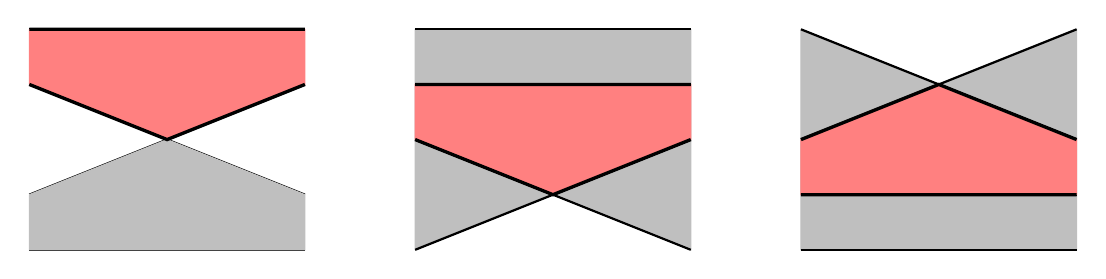
\begin{tikzpicture}[scale=.7]

{
\begin{scope} %Case 1: double convex
\draw[thick] (-2.5,2)--(2.5,2);
\draw[thick] (-2.5,-2)--(2.5,-2);
\draw[thick] (-2.5,-1)--(2.5,1);
\draw[thick] (2.5,-1)--(-2.5,1);

\draw[fill,red!50!white] (-2.5,1)--(0,0)--(2.5,1)--(2.5,2)--(-2.5,2)--(-2.5,1);
\draw[fill,gray!50!white] (-2.5,-1)--(0,0)--(2.5,-1)--(2.5,-2)--(-2.5,-2)--(-2.5,-1);
\draw[very thick] (-2.5,1)--(0,0)--(2.5,1) (-2.5,2)--(2.5,2);
\end{scope}
}
%
{
\begin{scope}[xshift=7cm,yshift=-1cm] % right hand diagram with 4 handle-slides
\draw[fill,gray!50!white] (-2.5,-1)--(0,0)--(2.5,-1)--(2.5,3)--(-2.5,3)--(-2.5,-1);


\draw[thick] (-2.5,3)--(2.5,3);
\draw[thick] (-2.5,-1)--(2.5,1);
\draw[thick] (2.5,-1)--(-2.5,1);

\draw[thick] (-2.5,2)--(2.5,2);
\draw[fill,red!50!white] (-2.5,1)--(0,0)--(2.5,1)--(2.5,2)--(-2.5,2)--(-2.5,1);


\draw[very thick] (-2.5,1)--(0,0)--(2.5,1) (-2.5,2)--(2.5,2);

\end{scope}
}
%%%
{
\begin{scope}[xshift=14cm,yshift=1cm] % right hand diagram with 4 

\draw[fill,gray!50!white] (-2.5,1)--(0,0)--(2.5,1)--(2.5,-3)--(-2.5,-3)--(-2.5,1);
\draw[thick] (-2.5,-1)--(2.5,1);
\draw[thick] (2.5,-1)--(-2.5,1);
\draw[thick] (-2.5,-2)--(2.5,-2);

\draw[thick] (-2.5,-3)--(2.5,-3);

\draw[fill,red!50!white] (-2.5,-1)--(0,0)--(2.5,-1)--(2.5,-2)--(-2.5,-2)--(-2.5,-1);


\draw[very thick] (-2.5,-1)--(0,0)--(2.5,-1) (-2.5,-2)--(2.5,-2);

\end{scope}
}

\end{tikzpicture}
\caption{The three possible configurations at a switch crossing. The higher-dimensional version is the product of this with a manifold. 
The two shadings denote the two $(n+1)$-manifolds characterizing the switch. In the local nested cases (2) and (3), the external grey $(n+1)$-manifold has a locally concave boundary.}
\label{fig: 3 cases of normal rulings}
\end{center}
\end{figure}
%
}

For the front projection of the Legendrian trefoil knot, Figure \ref{fig: Rulings}  illustrates two different rulings;  the shadings represent the rulings' $2$-manifolds.
 The unpaired sheet does not intersect the $2$-manifold at the switch, as stipulated in Definition \ref{def: Ruling}.4. 
In the left and center diagrams of Figure \ref{fig: St3}, the proposed ruling fails  Definition \ref{def: Ruling}.5: the upper blue line bounds a $3$-manifold whose boundary has a codimension-2 stratum at the triple point.
%
%For Legendrian knots, Definition \ref{def: Ruling} corresponds to what is called in the literature a {\em{graded normal ruling}} \cite{Sabloff}.
%The manifold condition is not part of this pre-existing definition in dimension 1, where it is automatically satisfied. \footnote{\color{red} Holds automatically in all dimensions?} 

Applications of these bounded $2$-manifolds have been studied, for example, in \cite{Kal06}. 

Various results relate counts/polynomials/categories of the knot's rulings, Chekanov-Eliashberg DGA augmentations, generating families, and constructible sheaves \cite{Fuchs03, FR11, S05, NS, NRSSZ}. 





{
%
\begin{figure}[htbp]
\begin{center}
{
%
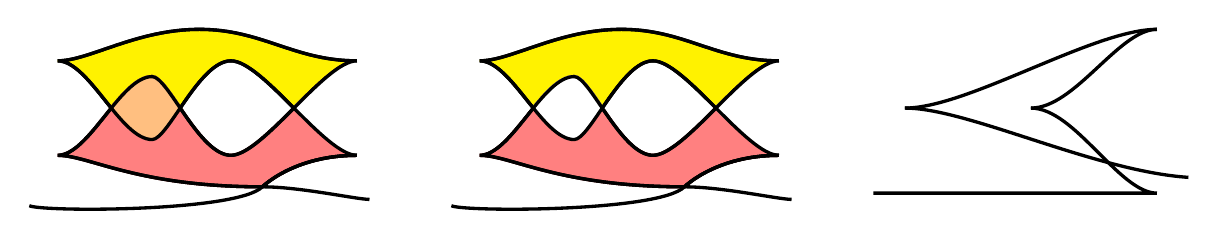
\begin{tikzpicture}[scale=.8]
%\draw[help lines=1,thick] (-5,-5) grid (5,4);
%
\begin{scope}[xshift=-7mm] % first
{
\begin{scope}[yshift=-2.5mm]
\draw[thick,fill, yellow] (5,1)..controls (4,1) and (3.5,1.5)..(2.5,1.5)..controls (1.5,1.5) and (.75,1)..(0.25,1)..controls (.75,1) and (1.25,-.25)..(1.75,-.25)..controls (2,-.25) and (2.5,1)..(3,1)..controls (3.5,1) and (4.5,-.5)..(5,-.5);
\draw[very thick] (5,1)..controls (4,1) and (3.5,1.5)..(2.5,1.5)..controls (1.5,1.5) and (.75,1)..(0.25,1)..controls (.75,1) and (1.25,-.25)..(1.75,-.25)..controls (2,-.25) and (2.5,1)..(3,1)..controls (3.5,1) and (4.5,-.5)..(5,-.5);
\end{scope}
%
\begin{scope}[yshift=2.5mm]
\draw[very thick,fill,red!50!white] (5,-1)..controls (4,-1) and (3.5,-1.5)..(3.5,-1.5)..controls (1.5,-1.5) and (.75,-1)..(0.25,-1)..controls (.75,-1) and (1.25,0.25)..(1.75,0.25)..controls (2,0.25) and (2.5,-1)..(3,-1)..controls (3.5,-1) and (4.5,.5)..(5,.5);

\draw[very thick] (5,-1)..controls (4,-1) and (3.5,-1.5)..(3.5,-1.5)..controls (1.5,-1.5) and (.75,-1)..(0.25,-1)..controls (.75,-1) and (1.25,0.25)..(1.75,0.25)..controls (2,0.25) and (2.5,-1)..(3,-1)..controls (3.5,-1) and (4.5,.5)..(5,.5);
\end{scope}


\draw[very thick,fill,white] (5.1,-.75)..controls (4.8,-.75) and (4.2,-.2) ..(4,0)..controls (4.2,.2) and (4.8,.75)..(5.1,.75);

\begin{scope}
\clip (0,0)rectangle (3,1);
\begin{scope}[yshift=2.5mm]
\draw[very thick,fill,orange!50!white] (5,-1)..controls (4,-1) and (3.5,-1.5)..(2.5,-1.5)..controls (1.5,-1.5) and (.75,-1)..(0.25,-1)..controls (.75,-1) and (1.25,0.25)..(1.75,0.25)..controls (2,0.25) and (2.5,-1)..(3,-1)..controls (3.5,-1) and (4.5,.5)..(5,.5);
\end{scope}
\end{scope}

\begin{scope}
\clip (0,0)rectangle (3,-1);
\begin{scope}[yshift=-2.5mm]
\draw[thick,fill, orange!50!white] (5,1)..controls (4,1) and (3.5,1.5)..(2.5,1.5)..controls (1.5,1.5) and (.75,1)..(0.25,1)..controls (.75,1) and (1.25,-.25)..(1.75,-.25)..controls (2,-.25) and (2.5,1)..(3,1)..controls (3.5,1) and (4.5,-.5)..(5,-.5);
\end{scope}
\end{scope}

\begin{scope}[yshift=-2.5mm]
\draw[very thick] (5,1)..controls (4,1) and (3.5,1.5)..(2.5,1.5)..controls (1.5,1.5) and (.75,1)..(0.25,1)..controls (.75,1) and (1.25,-.25)..(1.75,-.25)..controls (2,-.25) and (2.5,1)..(3,1)..controls (3.5,1) and (4.5,-.5)..(5,-.5);
\end{scope}


\begin{scope}[yshift=2.5mm]
\draw[very thick] (5,-1)..controls (4,-1) and (3.5,-1.5)..(3.5,-1.5)..controls (1.5,-1.5) and (.75,-1)..(0.25,-1)..controls (.75,-1) and (1.25,0.25)..(1.75,0.25)..controls (2,0.25) and (2.5,-1)..(3,-1)..controls (3.5,-1) and (4.5,.5)..(5,.5);
\end{scope}

\begin{scope}[yshift=2.5mm]
\draw[very thick] (3.5,-1.5)..controls (4.1,-1.5) and (5,-1.7)..(5.2,-1.7);
\end{scope}

\begin{scope}[yshift=2.5mm]
\draw[very thick] (5,-1)..controls (4,-1) and (3.5,-1.5)..(3.5,-1.5)..controls (3.1,-1.9) and (0,-1.9)..(-.2,-1.8);
\end{scope}

}
\end{scope}

\begin{scope}[xshift=6cm]% second
{
\begin{scope}[yshift=-2.5mm]
\draw[thick,fill, yellow] (5,1)..controls (4,1) and (3.5,1.5)..(2.5,1.5)..controls (1.5,1.5) and (.75,1)..(0.25,1)..controls (.75,1) and (1.25,-.25)..(1.75,-.25)..controls (2,-.25) and (2.5,1)..(3,1)..controls (3.5,1) and (4.5,-.5)..(5,-.5);
\draw[very thick] (5,1)..controls (4,1) and (3.5,1.5)..(2.5,1.5)..controls (1.5,1.5) and (.75,1)..(0.25,1)..controls (.75,1) and (1.25,-.25)..(1.75,-.25)..controls (2,-.25) and (2.5,1)..(3,1)..controls (3.5,1) and (4.5,-.5)..(5,-.5);
\end{scope}
%
\begin{scope}[yshift=2.5mm]
\draw[very thick,fill,red!50!white] (5,-1)..controls (4,-1) and (3.5,-1.5)..(3.5,-1.5)..controls (1.5,-1.5) and (.75,-1)..(0.25,-1)..controls (.75,-1) and (1.25,0.25)..(1.75,0.25)..controls (2,0.25) and (2.5,-1)..(3,-1)..controls (3.5,-1) and (4.5,.5)..(5,.5);

\draw[very thick] (5,-1)..controls (4,-1) and (3.5,-1.5)..(3.5,-1.5)..controls (1.5,-1.5) and (.75,-1)..(0.25,-1)..controls (.75,-1) and (1.25,0.25)..(1.75,0.25)..controls (2,0.25) and (2.5,-1)..(3,-1)..controls (3.5,-1) and (4.5,.5)..(5,.5);
\end{scope}


\draw[very thick,fill,white] (5.1,-.75)..controls (4.8,-.75) and (4.2,-.2) ..(4,0)..controls (4.2,.2) and (4.8,.75)..(5.1,.75);

\begin{scope}
\clip (0,0)rectangle (3,1);
\begin{scope}[yshift=2.5mm]
\draw[very thick,fill,white] (5,-1)..controls (4,-1) and (3.5,-1.5)..(2.5,-1.5)..controls (1.5,-1.5) and (.75,-1)..(0.25,-1)..controls (.75,-1) and (1.25,0.25)..(1.75,0.25)..controls (2,0.25) and (2.5,-1)..(3,-1)..controls (3.5,-1) and (4.5,.5)..(5,.5);
\end{scope}
\end{scope}

\begin{scope}
\clip (0,0)rectangle (3,-1);
\begin{scope}[yshift=-2.5mm]
\draw[thick,fill, white] (5,1)..controls (4,1) and (3.5,1.5)..(2.5,1.5)..controls (1.5,1.5) and (.75,1)..(0.25,1)..controls (.75,1) and (1.25,-.25)..(1.75,-.25)..controls (2,-.25) and (2.5,1)..(3,1)..controls (3.5,1) and (4.5,-.5)..(5,-.5);
\end{scope}
\end{scope}

\begin{scope}[yshift=-2.5mm]
\draw[very thick] (5,1)..controls (4,1) and (3.5,1.5)..(2.5,1.5)..controls (1.5,1.5) and (.75,1)..(0.25,1)..controls (.75,1) and (1.25,-.25)..(1.75,-.25)..controls (2,-.25) and (2.5,1)..(3,1)..controls (3.5,1) and (4.5,-.5)..(5,-.5);
\end{scope}

\begin{scope}[yshift=2.5mm]
\draw[very thick] (5,-1)..controls (4,-1) and (3.5,-1.5)..(3.5,-1.5)..controls (1.5,-1.5) and (.75,-1)..(0.25,-1)..controls (.75,-1) and (1.25,0.25)..(1.75,0.25)..controls (2,0.25) and (2.5,-1)..(3,-1)..controls (3.5,-1) and (4.5,.5)..(5,.5);
\end{scope}

\begin{scope}[yshift=2.5mm]
\draw[very thick] (3.5,-1.5)..controls (4.1,-1.5) and (5,-1.7)..(5.2,-1.7);
\end{scope}

\begin{scope}[yshift=2.5mm]
\draw[very thick] (5,-1)..controls (4,-1) and (3.5,-1.5)..(3.5,-1.5)..controls (3.1,-1.9) and (0,-1.9)..(-.2,-1.8);
\end{scope}
}
\end{scope}
%
\begin{scope}[xshift=13cm] % third
\draw[very thick] (0,0)..controls (1,0) and (3,-1)..(4.5,-1.1);
\draw[very thick] (0,0)..controls (1,0) and (3,1.25)..(4,1.25);
\draw[very thick] (2,0)..controls (2.7,0) and (3.4,-1.35)..(4,-1.35)--(-.5,-1.35);
\draw[very thick] (2,0)..controls (2.7,0) and (3.4,1.25)..(4,1.25);

\end{scope}
%\foreach \x in {-8,-6,...,8}\draw (\x,0) node{\x};\foreach \y in {-6,-4,...,8}\draw (0,\y) node{\y};
%\draw[thick,color=blue] (0,1) ellipse [x radius=2.8cm,y radius=2.1cm];
\end{tikzpicture}
}
\caption{Fronts in $J^0 S^1.$ On the left are two of the three possible rulings for a Legendrian trefoil knot. The stabilized unknot on the right has no rulings. Similarly, a loose \cite{Mur12} high-dimensional Legendrian admits no ruling.}
\label{fig: Rulings}
\end{center}
\end{figure}
%
}




The {\em{front-spin}} \cite{EES05a, Gol12} $\Lambda \times S^n$ has a canonical ruling given a ruling for $\Lambda.$



\subsection{Computing the torsion using handle-slides}
\label{sec: HandleSlides}


Recall the following notation\footnote{\color{red} Needs to be updated for consistency with new notation?} { \color{red} presumably now from Appendix 2} from Sections \ref{sec: fiber bundles} and \ref{sec: Reid inv}: $\Lambda \subset J^1 M$ has a generating function $f: W \rightarrow \bR$ where $F \rightarrow W \rightarrow M$ is a fiber bundle;
 $\Lambda$ has mild singularities { \color{red} mild should be changed to moderate everywhere or vice-versa}; there is a system of fiberwise Morse chain complexes {\color{red}  what about fiberwise metric?}
$CM_*(f_m; \bC^\rho)$ for $m \in M$ with coefficients in the trivial 1-dimension local system $\rho=1: \pi_1 W \rightarrow U(1).$ Thus 
\[
    CM_*(f_m; \bC^\rho)=CM_*(f_m; \bC)=CM_*(f_m; \bZ)\otimes \bC
\]
We now go into more details.



The generators of $CM_k(f_m)=CM_k(f_m; \bZ)$ are the set $\mbox{Crit}_k(f_m)$ of critical points of $f_m$ of Morse index $k.$
For each critical value $x \in \mbox{Crit}_k(f_m),$ the point $(m, f_m(x)) \in J^0(M)$ lies on one of the sheets of the front projection $\pi_F(\Lambda).$
To this sheet we can set the {{Maslov potential}} to be $k.$
Recall that a Maslov potential assignment is defined up to a global constant.
In particular, if we stabilize the generating family  $f(w)$ by $f(w) + u^2$ as in \color{red}Definition \ref{def: TwistedSister},\color{black} then this method for setting the Maslov potential of each sheet increases by 1.  



Given a ruling on the Legendrian $\Lambda$, we will show by an   {\em{explicit construction}} in Section \ref{sec: RulingTorsion}  that there exists a generating family $f(w)$ for $\Lambda$ which is ``framed up to sign"  which we will describe below. (Although Section \ref{sec: RulingTorsion} focuses on constructing generating families for a specific isotopy of a 2-copy of $\Lambda,$ it concludes with a generating family for the single copy as well.) 

Recall from  Section \ref{sec: fiber bundles} {\color{red} needs to be added to the appendix on functions with mild singularities} that a \emph{framed function} is a generalized Morse function (having only Morse and birth-death critical points) together with a framing of the descending manifold at each  (fiberwise)  critical point so  that:  at the cusps, the last vector of the framing is in the positive cubic direction;  this  framing extends continuously to the upper index critical point;  all but the last vector extend  continuously to the lower index critical point. We say that the function is \emph{framed up to sign} or \emph{almost framed} if the framing at a cusp is allowed to have the last vector being the negative cubic direction. 
 At such a cusp, the incidence number will be $-1$. {\color{red} let's just talk about this for a second} Furthermore, all incidences of the almost framed family of functions $f_m$ will also be framed up to sign; that is,  in a generic  level surface between two critical points of index $k,k+1$, the ascending sphere of the index $k$ critical point will have a normal framing coming from the framing of that critical point which  will intersect the descending $(k+1)$-disk $\bD^{k+1}$ of the other critical point at either  $e_{k+1} \in  \bD^{k+1} \subset \bR^{k+1}$  or $-e_{k+1}.$ The sign will be equal to the sign of the incidence assuming the $k$ vectors in the tangential framing of the descending $k$-sphere match the normal framing vectors of the ascending codimension-$k$ sphere. This condition will be satisfied in our Section \ref{sec: RulingTorsion} construction. 

To define the aforementioned ascending and descending manifolds, as well as the  differential $d_m$ of the complex $CM_*(f_m)$ when $m$ is away from the mild (birth-death) singularities, we need a vertical metric on $W,$ i.e., a metric on the vertical tangent space $T^vW,$ which is standard near $\mbox{Crit}_*(f_m).$ {\color{red} agreed — this should have been mentioned before. in fact, maybe a section on fiberwise metrics and fiberwise Morse homology can be added to Appendix A on functions with moderate singularities}  \footnote{\color{red}Metric should be mentioned in Section 2.2? Dec 2025: That was an old comment and may have been done, in which case this all can be a shortened review of notation.}
There is a stratification of $M$ such that for $m$ in the codimension-0 strata, $CM_*(f_m)$ is well-defined and continuous, i.e., the (integer entries of the matrix) of $d_m$ are constant, while the codimension-1 strata include the birth-deaths and failure of the fiber-wise Morse-Smale condition. Some of these latter codimension-1 strata are characterized by so-called {\em{handle-slides}}, which are gradient flow lines of $f_m$ starting and ending at $x,y \in \mbox{Crit}_k(f_m).$ {\color{red} this should maybe be in that aforementioned new section, also is there a reference for this? Kiyoshi's book?}
Similarly, using the language of Hatcher and Wagonner, there are some codimension-2 strata marking the locations of  {\em{exchanges}}, which are gradient flow lines starting at $x \in \mbox{Crit}_k(f_m)$ and ending at $y \in \mbox{Crit}_{k-1}(f_m).$ (We use the convention that the coefficient $\langle d_m(x), y \rangle$ is determined by flow lines starting at $x \in \mbox{Crit}_k(f_m)$ and ending at $y \in \mbox{Crit}_{k+1}(f_m).$)

 Handle-slides  and exchanges will be \emph{framed up to sign} in the Section \ref{sec: RulingTorsion} construction, which means  the following. 
For a handle-slide of index $k$ critical points $x,y$ with $f_m(x)<f_m(y)$, the ascending sphere going up from $x$ has codimension $k$ and is normally framed in any intermediate level surface. We require this sphere to cross the descending sphere $S^{k-1}=\partial \bD^k$, at the point corresponding to  
$e_k\in S^{k-1}  \subset \bD^k \subset \bR^k.$ 
The other $(k-1)$ tangential framing vectors $\xi_1,\cdots,\xi_{k-1}$ should match the first $(k-1)$ normal framing of the ascending sphere of $x$. The last normal framing vector $\xi_k$ should either match or be the negative of the velocity vector of moving descending sphere $S_y^{k-1}$ depending on the sign of the handle-slide. (By ``moving sphere" we mean the sphere in each fiber as the fiber moves over a curve transverse to the handle-slide stratum.) {\color{red} having a hard time following here, but maybe should match means should extend to framings that match, and also what happens in the unframed case?}
Note that  the sign of the handle-slide reverses when  the direction of movement is reversed. Exchange points will also be framed. The important thing for us is that the handle-slides emanating from the exchange point, as characterized in discussion ``(Exchange)" below, will be framed, not in general but in our Section \ref{sec: RulingTorsion} case.

{\color{red} there seems to be a lot of referencing future sections}

We refine the stratification to include the aforementioned handle-slide and exchange  strata, as well as the codimension-1 cusp and crossing loci introduced in Section \ref{sec: Rulings}.
We can assume that birth-deaths are independent in the sense of \cite{HW73}. {\color{red} maybe worth spelling out what this means}
In particular, a handle-slide and exchange stratum will not intersect a cusp-locus stratum, when one of the sheets used to define the cusp is associated with one of the ($\dim(M)$-family of fiberwise) critical points used to define the handle-slide or exchange. 



When $\dim(M) = 2,$ Hatcher and Wagonner prove that the handle-slide and exchange strata fit together according to Steinberg and exchange relations associated to 
codimension-2 strata \cite{HW73}. We review them now, letting  $e_{ij}^u$ denote  the elementary matrix with $u \in \bR$ in the $(i,j)$-entry, ones on the diagonal, and zero elsewhere.

\begin{enumerate}
\item[(St 1)] 
Suppose  critical points $i,j$ have the same index $n$, then the handle-slide $x_{ij}^u$ acts as a basis change operator on $CM_n(f_m).$
In $J^0(M),$ we denote the handle-slide as a vertical segment over each point of the handle-slide stratum. 
%
\begin{center}
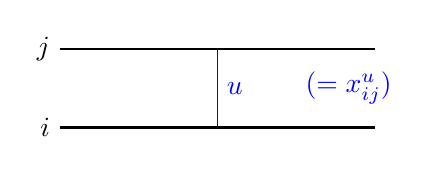
\begin{tikzpicture}%[scale=3]
%\draw[help lines=1,thick] (-5,-5) grid (5,4);
%\foreach \x in {-8,-6,...,8}\draw (\x,0) node{\x};\foreach \y in {-6,-4,...,8}\draw (0,\y) node{\y};
\draw[thick] (-2,1)--(2,1);
\draw[thick] (-2,0)--(2,0);
\draw (-2,0)node[left]{$i$};
\draw (-2,1)node[left]{$j$};
\draw[blue] (0,.5)node[right]{$u$};
\draw[blue] (1,.5)node[right]{$(=x_{ij}^u)$};

\draw[blue] (0,0)--(0,1);
\end{tikzpicture}
\end{center}
The chain complex $CM_{n+1}\xxrarrow{d_{n+1}} CM_{n}\xxrarrow{d_{n}} CM_{n-1}$ with $ d_n d_{n+1}=0$ 
becomes  $CM_{n+1}\xxrarrow{d_{n+1}'} CM_{n}\xxrarrow{d_{n}'} CM_{n-1}$   where $d_n'=d_ne_{ij}^u,$ $d_{n+1}'=e_{ij}^{-u}d_{n+1}
$ so that $d_n'd_{n+1}'=(d_ne_{ij}^{u})(e_{ij}^{-u}d_{n+1})=0$. The handle-slide $x_{ij}^u$ will be framed up to the sign $u=\pm1$. In the dual complex $CM_\ast^\ast=\mbox{Hom}(CM_\ast,\bZ)$, the incidence matrices are transposed: $d_n^\ast=d_n^t$ and the handle-slides are transposed and inverted since 
\[
(d_ne_{ij}^{u}e_{ij}^{-u}d_{n+1})^\ast=d_{n+1}^te_{ji}^{-u}e_{ji}^ud_n^t
\]
which is the handle-slide $x_{ji}^{-u}$.


\item[(St 2)]
If $i\neq \ell$, $j\neq k$ then the matrices $e_{ij}^u,e_{k\ell}^v$ commute. So the corresponding handle-slides commute. For example (for $\ell=j$) over two 1-dimensional slices of $M$ in $J^0(M),$ they appear as 
\begin{center}
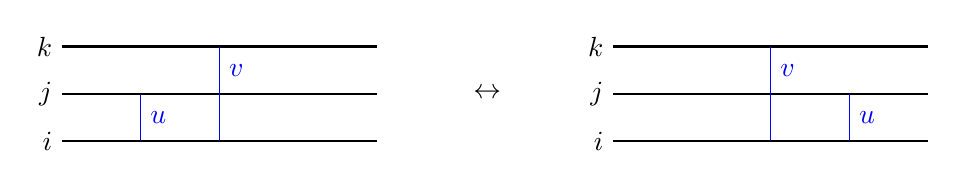
\begin{tikzpicture}[yscale=.6]
%\draw[help lines=1,thick] (-5,-5) grid (5,4);
%\foreach \x in {-8,-6,...,8}\draw (\x,0) node{\x};\foreach \y in {-6,-4,...,8}\draw (0,\y) node{\y};
\begin{scope}% left figure
\draw[thick] (-2,2)--(2,2);
\draw[thick] (-2,1)--(2,1);
\draw[thick] (-2,0)--(2,0);
\draw (-2,0)node[left]{$i$};
\draw (-2,1)node[left]{$j$};
\draw (-2,2)node[left]{$k$};
\draw[blue] (-1,.5)node[right]{$u$};
\draw[blue] (-1,0)--(-1,1);
\draw[blue] (0,1.5)node[right]{$v$};
\draw[blue] (0,0)--(0,2);
\end{scope}
%
\draw (3.4,1) node{$\leftrightarrow$};
%
\begin{scope}[xshift=7cm]% right figure
\draw[thick] (-2,2)--(2,2);
\draw[thick] (-2,1)--(2,1);
\draw[thick] (-2,0)--(2,0);
\draw (-2,0)node[left]{$i$};
\draw (-2,1)node[left]{$j$};
\draw (-2,2)node[left]{$k$};
\draw[blue] (1,.5)node[right]{$u$};
\draw[blue] (1,0)--(1,1);
\draw[blue] (0,1.5)node[right]{$v$};
\draw[blue] (0,0)--(0,2);
\end{scope}
\end{tikzpicture}
\end{center}

\item[(St 3)]
The matrix identity $e_{ij}^ue_{jk}^v=e_{jk}^ve_{ik}^{uv}e_{ij}^u$ when displayed as a handle-slide move is:
\begin{center}
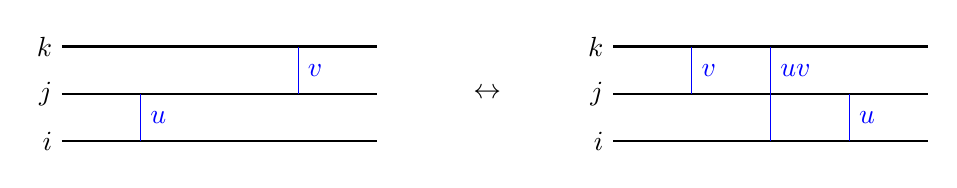
\begin{tikzpicture}[yscale=.6]
%\draw[help lines=1,thick] (-5,-5) grid (5,4);
%\foreach \x in {-8,-6,...,8}\draw (\x,0) node{\x};\foreach \y in {-6,-4,...,8}\draw (0,\y) node{\y};
\begin{scope}% left figure
\draw[thick] (-2,2)--(2,2);
\draw[thick] (-2,1)--(2,1);
\draw[thick] (-2,0)--(2,0);
\draw (-2,0)node[left]{$i$};
\draw (-2,1)node[left]{$j$};
\draw (-2,2)node[left]{$k$};
\draw[blue] (-1,.5)node[right]{$u$};
\draw[blue] (-1,0)--(-1,1);
\draw[blue] (1,1.5)node[right]{$v$};
\draw[blue] (1,1)--(1,2);
\end{scope}
%
\draw (3.4,1) node{$\leftrightarrow$};
%
\begin{scope}[xshift=7cm]% right figure
\draw[thick] (-2,2)--(2,2);
\draw[thick] (-2,1)--(2,1);
\draw[thick] (-2,0)--(2,0);
\draw (-2,0)node[left]{$i$};
\draw (-2,1)node[left]{$j$};
\draw (-2,2)node[left]{$k$};
\draw[blue] (1,.5)node[right]{$u$};
\draw[blue] (1,0)--(1,1);
\draw[blue] (0,1.5)node[right]{$uv$};
\draw[blue] (0,0)--(0,2);
\draw[blue] (-1,1.5)node[right]{$v$};
\draw[blue] (-1,1)--(-1,2);

\end{scope}
\end{tikzpicture}
\end{center}

\item[(Exchange)]
Suppose we have a (not necessarily square) matrix $R$ with $r_{ij}=0$. Then, for any $w$ in the coefficient ring (for us, the coefficient ring is $\bZ$ and we take $w=\pm1$) we have row operations equal to column operations:
\[
\prod_p e_{pi}^{r_{pj}w}R=R\prod_q e_{jq}^{wr_{iq}}
\]
This is called the {\emph{exchange relation}} $Z_{ij}^w$. 

In Morse theory, an exchange occurs when a trajectory appears going from an index-$(n+1)$ critical point $x_j$ up to an index-$n$ critical point $y_i$. In that case we necessarily have $r_{ij}=0$. When $r=I_2$ is the $2\times 2$ identity matrix, then $Z_{12}^w$ gives $I_2\to e_{21}^{-w}I_2\to e_{21}^{-w}I_2e_{21}^{w}$:

\begin{center}
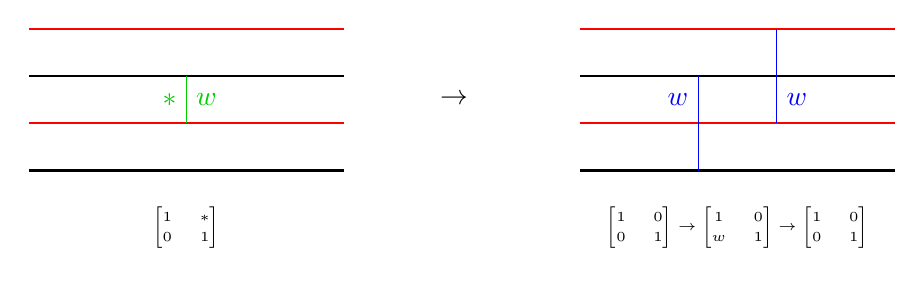
\begin{tikzpicture}[yscale=.6]%[scale=3]
\begin{scope}% left figure
\draw (0,-1.2)node{\tiny$\mat{1& \ast\\0&1}$};
\draw[thick,red] (-2,3)--(2,3);
\draw[thick] (-2,2)--(2,2);
\draw[thick,red] (-2,1)--(2,1);
\draw[thick] (-2,0)--(2,0);
\draw[green!80!black] (0,1.5)node[left]{$\ast$};
\draw[green!80!black] (0,1.5)node[right]{$w$};
\draw[green!80!black] (0,1)--(0,2);
\end{scope}
%
\draw (3.4,1.5) node{$\rightarrow$};
%
\begin{scope}[xshift=7cm]% right figure
\draw (0,-1.2)node{\tiny$\mat{1& 0\\0&1}\to \mat{1& 0\\w&1}\to \mat{1& 0\\0&1}$};

\draw[thick,red] (-2,3)--(2,3);
\draw[thick] (-2,2)--(2,2);
\draw[thick,red] (-2,1)--(2,1);
\draw[thick] (-2,0)--(2,0);

\draw[blue] (0.5,1.5)node[right]{$w$};
\draw[blue] (-0.5,0)--(-0.5,2);
\draw[blue] (-.5,1.5)node[left]{$w$};
\draw[blue] (.5,1)--(.5,3);
\end{scope}
\end{tikzpicture}
\end{center}
The first black over black handle-slide $x_{21}^w$ is left multiplication by $e_{21}^{-w}$ as in (St1) above.  
\end{enumerate}



When $\dim(M) \ge 2$, locally trivial products of these stratifications with $\bR^{\dim(M)-2}$ still hold. 
This can be proved either by studying parameterized intersection theory for stable and unstable manifolds, or by developing a parameterized Morse-Gromov compactification result. Rigorous proofs for the study of higher-codimension strata are being developed in \cite{KaracanThesis}. {\color{red} has this really not been done before? good for Karacan! important work}
We do not need to address such higher-codimension strata
 since our construction in Section \ref{sec: RulingTorsion} only uses the above-discussed Steinberg and exchange relations. 
% {\color{blue} Since, as we will show, the existence of a ruling will force the switch-crossing to be independent of each other which allows us to ignore the triple crossings of sheets and, also, the result of the deformation of the gradient vector field of $f_m$ that we will outline will result in the absence of exchanges or any Steinberg-3 relations. Note that we will not deform $f_m$, only the handle-slides.}


We next review a formula for \color{red} torsion that is alternate to Definition \ref{def: higher whitehead}. \color{black} {\color{red} not sure this is the right definition to reference}
 By assumption, $CM_\ast(f_m)$ has homology $\bZ$ in just one degree, say $n$. Thus there exists a chain homotopy equivalence $\varphi_m: \Sigma^n \bZ \rightarrow CM_\ast(f_m)$ where $\Sigma^n\bZ$ is the $n$-th suspension of the trivial $\bZ$ coefficient system on $M$. Let $\widetilde{CM}_\ast(f_m)$ be the mapping cone of $\varphi_m$. Then there is an exact sequence of chain complexes
\[
    0\to CM_\ast(f_m) \to \widetilde{CM}_\ast(f_m)\to \Sigma^{n+1}\bZ\to 0
\]
and $\widetilde{CM}_\ast(f_m)$ is acyclic (with zero homology). We need to extend the coefficients in two steps: from $\bZ$ to $\bR$, and then to $\bC$. The problem is that at a handle-slide $x_{ij}^u,$ the matrix for $d_m$ varies discontinuously in $m \in M.$ With coefficients in $\bR$, we can smoothly interpolate $u \in \bZ$ from 0 to $u$ in $\bR$. Then we extend to $\bC$. Let $\widetilde d_m$ be this new smoothly varying boundary map for the acyclic chain complex $\widetilde {CM}_\ast(f_m;\bC)$. Then
\[
    \widetilde d_m+\widetilde d_m^\ast: \bigoplus_k \widetilde {CM}_{2k} (f_m; \bC) \rightarrow  \bigoplus_k \widetilde {CM}_{2k-1} (f_m; \bC)
\]
will be a family of isomorphisms smoothly varying for $m\in M$. Here $\widetilde d_m^\ast$ is the transpose of $\widetilde d_m$ (equal to the conjugate transpose since $\widetilde d_m$ has real coefficients). Let
\[
    h=(\widetilde d_m+\widetilde d_m^\ast)^2=\widetilde d_m\widetilde d_m^\ast+\widetilde d_m^\ast\widetilde d_m:\widetilde C_{even}\cong\widetilde C_{odd}
\]
Since $h$ is positive definite Hermitian, write $h = Q D Q^{-1}$ where $Q$ is unitary and $D$ is diagonal with positive eigenvalues. Let $h^\lambda = Q D^\lambda Q^{-1},$ which is still positive Hermitian for any $\lambda\in\bR$.

\begin{theorem}[\cite{I02}]
\label{thm: AlternativeTorsion}
Suppose  $\widetilde C_{even} = \widetilde C_{2i}, \widetilde C_{odd} = \widetilde C_{2i-1}$ for some choice of integer $i.$
Then an alternate formula for the torsion is
$$
wh_i(\widehat{f})  = \mbox{Trace} \int_0^1 \left( h^{-\lambda} d h^{-\lambda} \right)^{4i+1} d \lambda $$
\end{theorem}

{\color{red} I think this should now be $\tau_i(f)$ or something like that based on the notation of Appendix B}

(There is a correction term to this formula which lies in the image of the Pontrjagin character: $p:KO^0(S^{4i}) \to H^{4i}(S^{4i};\bR)$, see Section \ref{sec: main results}. {\color{red} this should now presumably reference the framing principle of appendix B}  In the case when $f_m$ is framed or almost framed this correction term is zero  \cite{I02}.) This integral version of torsion suggests that torsion computations can be reduced to studying codimension-$4i$ strata of the system of fiberwise Morse chain complexes.
In particular, we need in Section \ref{sec: RulingTorsion} the following.




\begin{lemma}\label{block diagonal h}
Assume the hypothesis of Theorem \ref{thm: AlternativeTorsion}.
If the matrix $h$ is locally in block diagonal form with fewer than $4i$ variable in each block, then the higher torsion form is identically zero.
\end{lemma}

\begin{proof}
The matrix 1-form $\omega=h^{-\lambda}dh^\lambda$ is also in block diagonal form. The trace of $\omega^{4i+1}$ is the sum of traces of the blocks raised to the power $4i+1$. But if a block of $h$ has $j<4i$ variables, the corresponding block of $\omega$ will have $j+1<4i+1$ variables. So the trace of $\omega^{4i+1}$ will be zero.
\end{proof}

%\color{blue}
%In our case, there is locally only one degree of freedom. So the torsion form $wh_k(\widehat f)$ will be zero. 
%\color{red} [I stated Cor \ref{cor: NoCodim4} more generally in case we ever relax ruling definition, but you change it if you want. This ``one degree" comment should probably go in Part 2e.] \color{black}



\begin{corollary}
\label{cor: NoCodim4}
\color{red} Consider a Legendrian as in Theorem \ref{thm: VanishingTorsion} and its generating function of tube type. \color{black}
Suppose the Legendrian has a Maslov potential supported in two consecutive integers. 
Suppose the strata are only defined by (almost) framed handle-slides, crossings, cusps, and intersections thereof.
Suppose that there are no intersections of four handle-slide strata, such that over any point in this intersection, when representing each handle-slide as a vertical segment in $J^0(M),$ the union of the four segments is connected. 
Then the torsion $wh_i(\widehat{f})$ vanishes. 
\end{corollary}

{\color{red} this is an interesting result that merits some more spotlight I think. In particular maybe spelling out the last hypothesis and giving it a name could be worth it} 


 \subsection{A special case of Theorem \ref{thm: VanishingTorsion}}
 \label{sec: RulingTorsion}
 

In this section we prove  Theorem \ref{thm: VanishingTorsion} when the Legendrian's Maslov potential is restricted to two consecutive integers. The following is a summary of the proof.

 
%We can now state and prove the result for our main class of examples.
Let $\Lambda \subset J^1 M$ be the Legendrian lift of a nearby Lagrangian in $T^\ast M.$
$\Lambda$ admits a generating family, see Section \ref{sec: class}.
The first author's PhD thesis implies that $\pi_F(\Lambda)$ has only mild front singularities \cite{AG18b}.  {\color{red} IT DOES NOT, this is know when $\Lambda$ has the homotopy type of a sphere and for arbitrary $\Lambda$ is the subject of my student P. Benk's PhD thesis, still very much in progress}
So, as explained in Section \ref{sec: HandleSlides}, we will construct a generating family for $\Lambda$ which is an almost framed function.
% and assume that $\pi_F(\Lambda)$ has mild singularities in order to compute its higher torsion from the loci of handle-slides. 
%
%First we need a 1-parameter version of the Ferrand-Chekanov construction for generating families \cite{}.
%Suppose, for $t \in [0,1],$ $\Lambda_t \subset J^1M$ is a Legendrian isotopy of mild Legendrians.
%Suppose $f_0$ is a generating family for $\Lambda_0$ with only handle-slides and exchanges (nothing higher), which we denote by
%$\mathcal{M}_0.$ 
%Suppose $\mathcal{M}_t$ is a possible extension of the handle-slides and exchanges, consistent with $\pi_F(\Lambda_t)$ as  described in Section \ref{sec: HandleSlides}.
%
%
%\begin{lemma}
%\label{lem: FerrandChekanov}
%There exists a 1-parameter family $f_t$ of generating families for $\Lambda_t$ whose actual handle-slides and exchanges coincide with $\mathcal{M}_t.$
%\end{lemma}
%
%\begin{proof}
%\color{red} Do the Ferrand-Chekanov construction inductive in time $t.$
%This should be automatic when nothing [like (St2), etc] happens.
%At a singular moment $t_0$ this should also be automatic away (in space) from where the singular event occurs. Maybe a case-by-case study of local (in space) of singular events, but I think it should also be automatic there too, no? \color{black}
%\end{proof}
%
\color{red} As in Section \ref{sec: DoublingConstruction}, \color{black} we consider a 2-copy  $\Lambda \cup \Lambda_t$ with the second copy $\Lambda_t$ slightly shifted by $t >0$ in the vertical $z$-direction. 
%Because $\Lambda$ is the lift of a nearby Lagrangian, $\Lambda \cup \Lambda_t$ is always embedded.
In Part 1 of the proof, we construct a generating family for $\Lambda \cup \Lambda_t.$
We use the ruling hypothesis to study what happens to certain almost framed handle-slides, which are fully understood when $t$ is small but less so for increasingly large $t.$
Once $t$ is large enough and $\min z(\Lambda_t) > \max z(\Lambda),$ our generating family for $\Lambda \cup \Lambda_t$ can be cut-off to create a generating family for $\Lambda.$
In Part 2, we give a complete accounting of the handle-slides during the isotopy.
 When Corollary \ref{cor: NoCodim4} applies, this accounting is sufficient to conclude
 that the torsion of this cut-off generating family of $\Lambda$ vanishes.
\color{red} The function in natural by Definition \ref{def: natural}. \color{black}

 {\color{red} I don't understand this, why is it natural by Definition \ref{def: natural}? that's just stating the definition. from the construction below it is not clear to me the construction is natural — needs to be discussed }
 
 \smallskip
 
  \noindent
 {\bf{Part 1:}} Constructing generating families framed up to sign for a vertical shift of a 2-copy.
 
 \smallskip
 

 
 


 
 
 
 \smallskip
 
  \noindent
 {\bf{Part 1a:}} Constructing the initial generating family at time $t=\epsilon <<1.$
 
 \smallskip
 

 
The link $\Lambda \cup \Lambda_\epsilon$ has a well-known generating family which we  describe in Figures \ref{fig: doubling L, make 8}
and \ref{fig: doubling L}.
The two handle-slides drawn can be made arbitrarily close to the crossing loci and each represent a manifold of handle-slides diffeomorphic to the cusp locus. Moreover, there are no other handle-slides.

\color{red}
If $\pi_F(\Lambda)$ has no cusps, we can reduce it to the case when it does, after a $C^2$-small isotopy  supported near a point which creates for $\pi_F(\Lambda)$ the product of a swallowtail with $S^{n-1}$. 
(In Section \ref{sec: RulingGeneratingFamily}, $\Lambda$ might not be a lift of a nearby Lagrangian and so might have multiple components. In which case, we perform this small isotopy to each component.)
Alternatively, without such an isotopy, $\Lambda \cup \Lambda_\epsilon$ has a tautological generating family with  a dimension-1 fiber where the fiber-index 0 (resp. 1) critical points of $f_m$ correspond to $\Lambda$ (resp. $\Lambda_\epsilon$) over $m \in M.$
\color{black}

{\color{red} I'm confused about this Legendrian without cusps. doesn't seem that interesting to us. I guess Legendrian braids type of thing?}

 {
%
\begin{figure}[htbp]
\begin{center}
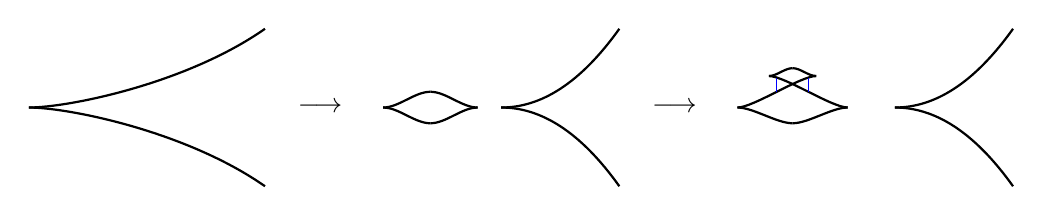
\begin{tikzpicture}%[scale=3]
%\draw[help lines=1,thick] (-1,-3) grid (12,3);
%\foreach \x in {-8,-6,...,8}\draw (\x,0) node{\x};
%\foreach \x/\y in {(0,1)/3,(0,0)/1,(0,-1)/2}
%\foreach \y in {-1,...,3}\draw (0,\y) node{\y};
%\coordinate (A) at (0,0);
\begin{scope}[xshift=-5mm]
\draw[thick] (0,0)..controls (.5,0) and (2,.3)..(3,1);
\draw[thick] (0,0)..controls (.5,0) and (2,-.3)..(3,-1);
\end{scope}
\draw (3.2,0) node{$\longrightarrow$};
%
\begin{scope}[xshift=4cm]
\draw[thick] (0,0) .. controls (.2,0) and (.4,.2)..(.6,.2);
\draw[thick] (0,0) .. controls (.2,0) and (.4,-.2)..(.6,-.2);
\draw[thick] (1.2,0) .. controls (1,0) and (.8,.2)..(.6,.2);
\draw[thick] (1.2,0) .. controls (1,0) and (.8,-.2)..(.6,-.2);
\draw[thick] (1.5,0)..controls (2,0) and (2.5,.3)..(3,1);
\draw[thick] (1.5,0)..controls (2,0) and (2.5,-.3)..(3,-1);
\end{scope}
%
\draw (7.7,0) node{$\longrightarrow$};
%
\begin{scope}[xshift=8.5cm]
\draw[thick] (0,0) .. controls (.2,0) and (.8,.4)..(1,.4);
\draw[thick] (0,0) .. controls (.2,0) and (.5,-.2)..(.7,-.2);
\draw[thick] (1.4,0) .. controls (1.2,0) and (.6,.4)..(.4,.4);
\draw[thick] (1.4,0) .. controls (1.2,0) and (.9,-.2)..(.7,-.2);
\draw[thick] (.4,.4) ..controls (.5,.4) and (.6,.5) .. (.7,.5);
\draw[thick] (1,.4) ..controls (.9,.4) and (.8,.5) .. (.7,.5);
\draw[blue] (0.5,.2)--(0.5,.38);
\draw[blue] (0.9,.2)--(0.9,.38);
\end{scope}

\begin{scope}[xshift=9cm]
\draw[thick] (1.5,0)..controls (2,0) and (2.5,.3)..(3,1);
\draw[thick] (1.5,0)..controls (2,0) and (2.5,-.3)..(3,-1);
\end{scope}
%\draw[thick,color=blue] (A) ellipse [x radius=2.8cm,y radius=2.1cm];
\end{tikzpicture}
\caption{%Doubling the front projection of a Lagrangian $\Lambda$ in $M\times \mathbb R$, Step 1: 
Pinch off an annulus along the cusp sets then introduce a swallowtail on the top sheet of the annulus, producing a ``figure 8'' along the cusp locus.
}
\label{fig: doubling L, make 8}
\end{center}
\end{figure}
%

}
 
{
%
\begin{figure}[htbp]
\begin{center}
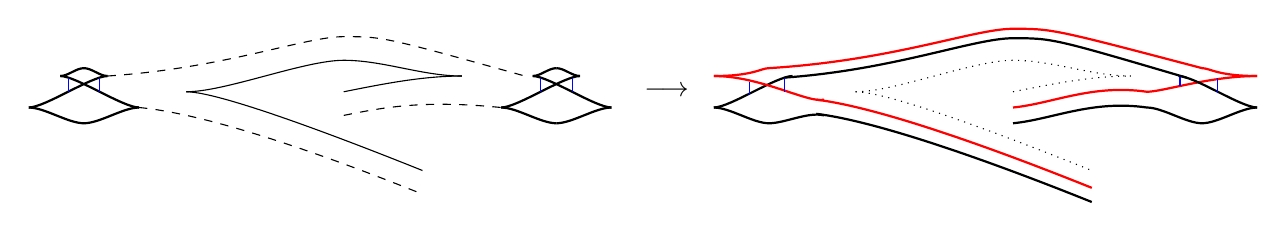
\begin{tikzpicture}%[scale=3]
%\draw[help lines=1,thick] (-1,-3) grid (12,3);
%\foreach \x in {-8,-6,...,8}\draw (\x,0) node{\x};
%\foreach \x/\y in {(0,1)/3,(0,0)/1,(0,-1)/2}
%\foreach \y in {-1,...,3}\draw (0,\y) node{\y};
%\coordinate (A) at (0,0);
\begin{scope}[xshift=8.5cm]
\begin{scope}[yshift=6mm]% top red sheet
\draw[thick,red] (.4,-.1)..controls (2,0) and (3,.4)..(3.5,.4)..controls (4,.4) and (4,.4)..(5.9,-.1);
%\draw (3.5,0)..controls (4,0.1) and (4.5,.2)..(5,.2);
%\draw (1.5,0)..controls (2,0) and (4,-.8)..(4.5,-1);
\end{scope}
\begin{scope}[yshift=4.8mm]% black top sheet
\draw[thick] (.6,-.1)..controls (2,0) and (3,.4)..(3.5,.4)..controls (4,.4) and (4,.4)..(5.7,-.1);
%\draw (3.5,0)..controls (4,0.1) and (4.5,.2)..(5,.2);
%\draw (1.5,0)..controls (2,0) and (4,-.8)..(4.5,-1);
\end{scope}

\begin{scope}[xshift=-3mm] % top of 8 on left
\draw[thick] (0,0) .. controls (.2,0) and (.8,.4)..(1,.4);
\draw[thick] (0,0) .. controls (.2,0) and (.5,-.2)..(.7,-.2);
\draw[thick,red] (1.4,0.1) .. controls (1.2,0.05) and (.6,.4)..(0,.4);
\draw[thick] (1.4,-.1) .. controls (1.2,-.05) and (.9,-.2)..(.7,-.2);
\draw[thick,red] (0,.4) ..controls (.5,.4) and (.6,.5) .. (.7,.5);
%\draw[thick] (1,.4) ..controls (.9,.4) and (.8,.5) .. (.7,.5);
\draw[blue] (0.45,.16)--(0.45,.33);
\draw[blue] (0.9,.2)--(0.9,.38);
\end{scope}

\begin{scope}[yshift=2mm]
\draw[thin,dotted] (1.5,0)..controls (2,0) and (3,.4)..(3.5,.4)..controls (4,.4) and (4.5,.2)..(5,.2);
\draw[thin,dotted] (3.5,0)..controls (4,0.1) and (4.5,.2)..(5,.2);
\draw[thin,dotted] (1.5,0)..controls (2,0) and (4,-.8)..(4.5,-1);
\end{scope}

\begin{scope}[xshift=5.2cm]% top of 8 on right 
\draw[thick,red] (0,0.2) .. controls (.2,0.2) and (.8,.4)..(1.4,.4);
\draw[thick] (0,0) .. controls (.2,0) and (.5,-.2)..(.7,-.2);
\draw[thick] (1.4,0) .. controls (1.2,0) and (.6,.4)..(.4,.4);
\draw[thick] (1.4,0) .. controls (1.2,0) and (.9,-.2)..(.7,-.2);
%\draw[thick] (.4,.4) ..controls (.5,.4) and (.6,.5) .. (.7,.5);
\draw[thick,red] (1.4,.4) ..controls (.9,.4) and (.8,.5) .. (.7,.5);
\draw[blue] (0.9,.18)--(0.9,.38);
\draw[blue] (0.42,.27)--(0.42,.39);
\end{scope}

\begin{scope}[yshift=-1mm]%black right
\draw[thick] (3.5,-.1)..controls (4,-0.05) and (4.5,.2)..(5.2,0.1);
\end{scope}
\begin{scope}[yshift=1mm]%black right
\draw[thick,red] (3.5,.-.1)..controls (4,-0.05) and (4.5,.2)..(5.2,0.1);
\end{scope}


\begin{scope}[yshift=-2mm]
\draw[thick] (1,0.12)..controls (2,0) and (4,-.8)..(4.5,-1);
\end{scope}


\begin{scope}[yshift=-.2mm]
\draw[thick,red] (1,0.12)..controls (2,0) and (4,-.8)..(4.5,-1);
\end{scope}


\end{scope}



\draw (7.6,.2) node{$\longrightarrow$};
%%%%%%%%%%%%%%%%%%%%%%%%%
\begin{scope}%[xshift=8.5cm]
\begin{scope}[xshift=-5mm]% top of 8 on left
\draw[thick] (0,0) .. controls (.2,0) and (.8,.4)..(1,.4);
\draw[thick] (0,0) .. controls (.2,0) and (.5,-.2)..(.7,-.2);
\draw[thick] (1.4,0) .. controls (1.2,0) and (.6,.4)..(.4,.4);
\draw[thick] (1.4,0) .. controls (1.2,0) and (.9,-.2)..(.7,-.2);
\draw[thick] (.4,.4) ..controls (.5,.4) and (.6,.5) .. (.7,.5);
\draw[thick] (1,.4) ..controls (.9,.4) and (.8,.5) .. (.7,.5);
\draw[blue] (0.5,.2)--(0.5,.38);
\draw[blue] (0.9,.2)--(0.9,.38);
\end{scope}




\begin{scope}[yshift=2mm]
\draw (1.5,0)..controls (2,0) and (3,.4)..(3.5,.4)..controls (4,.4) and (4.5,.2)..(5,.2);
\draw (3.5,0)..controls (4,0.1) and (4.5,.2)..(5,.2);
\draw (1.5,0)..controls (2,0) and (4,-.8)..(4.5,-1);
\end{scope}
%
\begin{scope}[yshift=5mm]
\draw[dashed] (.5,-.1)..controls (2,0) and (3,.4)..(3.5,.4)..controls (4,.4) and (4,.4)..(5.8,-.1);
\end{scope}

\begin{scope}[yshift=-1mm]
\draw[dashed] (3.5,0)..controls (4,0.1) and (4.5,.2)..(5.5,0.1);
\draw[dashed] (.9,0.1)..controls (2,0) and (4,-.8)..(4.5,-1);
\end{scope}



\begin{scope}[xshift=5.5cm]%top of 8 on right
\draw[thick] (0,0) .. controls (.2,0) and (.8,.4)..(1,.4);
\draw[thick] (0,0) .. controls (.2,0) and (.5,-.2)..(.7,-.2);
\draw[thick] (.4,.4) ..controls (.5,.4) and (.6,.5) .. (.7,.5);
\draw[thick] (1,.4) ..controls (.9,.4) and (.8,.5) .. (.7,.5);
\draw[thick] (1.4,0) .. controls (1.2,0) and (.6,.4)..(.4,.4);
\draw[thick] (1.4,0) .. controls (1.2,0) and (.9,-.2)..(.7,-.2);
\draw[blue] (0.5,.2)--(0.5,.38);
\draw[blue] (0.9,.2)--(0.9,.38);
\end{scope}
\end{scope}

%\draw[thick,color=blue] (A) ellipse [x radius=2.8cm,y radius=2.1cm];
\end{tikzpicture}
\caption{Take the top new inner cusp and stretch it along the top sheet of $\Lambda$. Take the bottom inner cusp and stretch it along the bottom sheet. The doubled Legendrian $\Lambda \cup \Lambda_\epsilon$ has a generating function with handle-slides shown by vertical blue lines, running between sheets of the same Maslov potential.
}
\label{fig: doubling L}
\end{center}
\end{figure}
%

}
 
 

The {\em{incidence matrices}} are the fiber differentials $d_m$ of $CM_*(f_m,\bC)$ when written with respect the canonical basis generated by the fiber critical points.
When $m$ lies outside some small tubular neighborhood of the handle-slides (which includes the crossings but not the cusps), the incidence matrices have a single non-zero entry in each row and column. 
Away from the cusp strata these are the row and column for corresponding red-black paired sheets of the black $\Lambda$ and red $\Lambda_\epsilon$ in Figure \ref{fig: doubling L}.
Near the cusp strata these are the row and column for the two cusping sheets. 
%\color{red}
We can ensure the matrix is this sparse, at least initially, by placing the pair of fiber critical points (same color near cusp, different colors away from cusp) in their own $\bR^2$-factor of the $\bR^N$ fiber.
This means they are the only critical points with non-zero coordinates in this factor, and the gradient flow connecting them is the only flow with said non-zero coordinates.
Note that in the neighborhood of the handle-slides, the four relevant fiber critical points sit in their own $\bR^4$-factor.

{\color{red} this is a bit too informal for my taste, and in any case I don't quite follow. is there a way to make it more precise? what if a same sheet goes back over itself (i.e. over a point of $M$ where the sheet has multiple preimages). more rigor would help clarify}

We construct the ``figure 8'' using a standard model and spin it along the cusp locus. This will have a framing up to sign and  by a calculation similar to the one in Figure \ref{Fig: figure 8 and mirror} below we see that the product of the signs at the 4 cusps must be negative. 
So, there is an odd number of negative signs. We can choose the inner cusps to be positive and either the top or bottom cusp on the outside will be negative depending on the ruling as we explain   towards the end of Step 1a. See Figure \ref{Fig: figure 8 and mirror} for a simple example. 

{
\begin{figure}[htbp]

\begin{center}
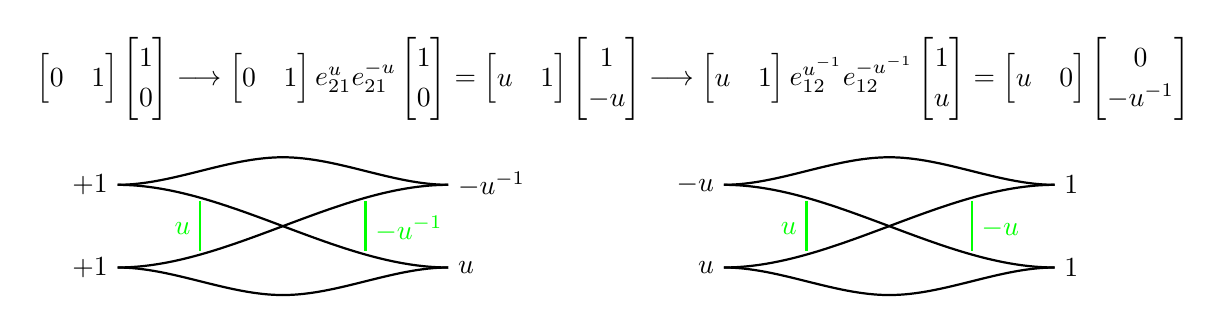
\begin{tikzpicture}[scale=.7]

\draw (0,2.5) node[above]{$\mat{0&1}\mat{1\\0}\longrightarrow \mat{0&1}e_{21}^{u }e_{21}^{-u}\mat{1\\0}=\mat{u&1}\mat{1\\-u}
\longrightarrow \mat{u&1}e_{12}^{u^{-1}}e_{12}^{-u^{-1}}\mat{1\\u}=\mat{u&0}\mat{0\\-u^{-1}}
$};
{
\begin{scope}[xshift=-9cm]
\draw[thick] (0,0)..controls (1,0) and (2,-.5)..(3,-.5);
\draw[thick] (6,0)..controls (5,0) and (4,-.5)..(3,-.5);
%
\draw[thick] (0,1.5)..controls (1,1.5) and (2,2)..(3,2);
\draw[thick] (6,1.5)..controls (5,1.5) and (4,2)..(3,2);
%
\draw[thick] (0,0)..controls(2,0)and(4,1.5)..(6,1.5);
\draw[thick] (6,0)..controls(4,0)and(2,1.5)..(0,1.5);
\draw (0,0) node[left]{+1};
\draw (0,1.5) node[left]{+1};
\draw (6,0) node[right]{$u$};
\draw (6,1.5) node[right]{$-u^{-1}$};
%
\draw[green,thick] (1.5,.3)--(1.5,1.2);
\draw[green,thick] (4.5,.3)--(4.5,1.2);
\draw[green] (1.5,.7)node[left]{$u$};
\draw[green] (4.5,.7)node[right]{$-u^{-1}$};
\end{scope}
}

{
\begin{scope}[xshift=2cm]
\draw[thick] (0,0)..controls (1,0) and (2,-.5)..(3,-.5);
\draw[thick] (6,0)..controls (5,0) and (4,-.5)..(3,-.5);
%
\draw[thick] (0,1.5)..controls (1,1.5) and (2,2)..(3,2);
\draw[thick] (6,1.5)..controls (5,1.5) and (4,2)..(3,2);
%
\draw[thick] (0,0)..controls(2,0)and(4,1.5)..(6,1.5);
\draw[thick] (6,0)..controls(4,0)and(2,1.5)..(0,1.5);
\draw (0,0) node[left]{$u$};
\draw (0,1.5) node[left]{$-u$};
\draw (6,0) node[right]{$1$};
\draw (6,1.5) node[right]{$1$};
%
\draw[green,thick] (1.5,.3)--(1.5,1.2);
\draw[green,thick] (4.5,.3)--(4.5,1.2);
\draw[green] (1.5,.7)node[left]{$u$};
\draw[green] (4.5,.7)node[right]{$-u$};
\end{scope}
}
%
\end{tikzpicture}
\caption{We have a ``figure 8'' and its mirror image. Here $u$ will be $\pm1$ and $-u^{-1}=-u$. Signs of handle-slides change in the mirror. Above the two figure 8's is the sequence of incidence matrices given by the handle-slides in the first figure 8. The same sequence in reverse corresponds to the second figure 8.}
\label{Fig: figure 8 and mirror}
\end{center}
\end{figure}
}

Along each of the inward pointing cusps we have, in local coordinates, the framed function 
\[
f_s(x)=f_0(0)+x_j^3-sx_j-\sum_{i<j} x_i^2+\sum_{k>j} x_k^2
\]
where $s$ is the coordinate orthogonal to the cusp. 
The first $j$ coordinates give the positive framing at the cusp. Assuming that we have stabilized enough so that $0<<j<<N$ where $N$ is the fiber direction, the space of $j$-frames in $\bR^N$ will be highly connected. 
Along the dotted lines in Figure \ref{fig: doubling L}, we take a path in the space of $j$-frames, then use those local coordinates to construct the pair of cancelling framed Morse critical points as shown in Figure \ref{fig: doubling L}.

We choose $u=1$ or $-1$ as follows.  Here is where we first use the ruling. Pick a cusp and set $u=1$ there. Extend continuously along the cusp strata. If the $(n+1)$-manifold associated to that cusp has only one cusp component, then pick a point on another cusp strata, set $u=1$ there and proceed as with the previous cusp. 
If the $(n+1)$-manifold has another cusp component, put $u=(-1)^m$ there; here, $m$ is the number of 
times a path on the boundary of the $(n+1)$-manifold, connecting the two cusp components, crossed a switch while sitting on the manifold associated to that switch.
See Definition \ref{def: Ruling} for a reminder of ``associated manifolds." 
%upward convex switches plus the number of nested convex switches along a path on the boundary of the $(n+1)$-manifold connecting the two cusp components. 
%(See Figure \ref{fig: 3 cases of normal rulings} for convex, concave and nested.)
This is independent of the choice of paths due to the vanishing $\bZ_2$-cohomological condition in Definition \ref{def: Ruling}. 





%{\color{blue}
%
%Along the parameter domain of the ruling, we assign signs $\pm1$ which change at those convex crossings mentioned above. Sometimes the sign does not change. For example if the crossing is concave or if it is the lower convex crossing which is not nested. In the regions between any switching crossings (ones where the ruling switches sheets), we introduce handle-slides as follows.
%
%Take the level surface $L$ between the bottom of the upper sheet and the top of the lower sheet of the ruling. Then $L$ is $N-1$ dimensional and highly connected. The descending manifold of the upper sheet pair is a $j$-disk which is tangentially framed, i.e., diffeomorphic to the standard $j$-disk by the positive framing. The lower pair of sheets give an $N-j$ disk which is normally framed.
%%
%\begin{figure}[htbp]
%\begin{center}
%\begin{tikzpicture}[scale=1.5]
%\draw[fill,red!50!white] (0,0)circle[radius=5mm];
%\draw[thick,red!40!black] (0,0)circle[radius=5mm];
%\draw[very thick,red!40!black] (0,0)--(.5,0);
%\draw[fill,blue!50!white] (1.5,0)circle[radius=5mm];
%\draw[very thick,blue!50!black](1.5,0)circle[radius=5mm];
%%
%\begin{scope}[xshift=5cm]
%\draw[fill,red!50!white] (0,0)circle[radius=5mm];
%\draw[thick,red!40!black] (0,0)circle[radius=5mm];
%\draw[very thick,red!40!black] (0,0)--(.5,0);
%
%\draw[fill,blue!50!white] (.5,0)ellipse[x radius=5mm,y radius=3mm];
%\draw[very thick,blue!50!black] (.5,0)ellipse[x radius=5mm,y radius=3mm];
%
%
%\begin{scope}
%\clip (-1,0)rectangle (1,1);
%\draw[fill,red!50!white] (0,0)circle[radius=5mm];
%\draw[thick,red!40!black] (0,0)circle[radius=5mm];
%\draw[very thick,red!40!black] (0,0)--(.5,0);
%\end{scope}
%
%\end{scope}
%\end{tikzpicture}
%\caption{The descending $j$-disk is in red. The line to the center of the red disk indicates the positive or negative $x_j$ direction depending on the designated sign of the ruling at that point. The ascending $N-j$ disk is blue. The moment that the two boundaries cross is where the handle-slide occurs. That handle-slide will be positive or negative depending on the designated sign. The disks come apart along the boundary of that component. This causes a handle-slide with the correct sign to appear on either side of a switching crossing.}
%\label{fig: disks crossing in $L$}
%\end{center}
%\end{figure}
%%
%%
%}
%\color{red} [Describe how the ``fiber lab containment property"  ensures this. Do we need to discuss the fiberwise vertical metrics at this point?] \color{black}
 
%To build a generating family for $\Lambda \cup \Lambda_t,$ we use Chekanov's construction \cite{Chekanov96}, made more explicit by Ferrand \cite[Proposition 5]{Ferrand97}. They use a fragmentation of a contact isotopy which induces the Legendrian isotopy; that is, they write the contact isotopy as a concatenation of $C^1$-small isotopies each with small compact support; see \cite[Lemma 13]{Ferrand97} for the formula of such $C^1$-small isotopies. When we adopt this, our Legendrian isotopy is only $C^1$-approximately a global vertical shift; however, this limitation does not affect our proof.

%The Chekanov-Ferrand construction is not enough since we need some control of the change in fiberwise gradient flow trajectories, in addition to the front, as $t$ increases from $\epsilon$ to $N.$ 
%This relies on prescribing how the fiberwise vertical metrics change with $t.$


\smallskip
 
  \noindent
 {\bf{Part 1b:}} Constructing the generating families when $\epsilon \le t \le 2 \epsilon.$ 
 
 \smallskip

Each crossing stratum that defines a switch in Definition \ref{def: Ruling} 
has two isomorphic crossing strata between sheets of $\Lambda$ and $\Lambda_\epsilon.$  
The manifold \color{red} boundary's \color{black} property in the ruling ensures that the switch crossing stratum is a codimension-1 closed manifold $X$; for example, the crossing stratum does not have a boundary at some cusp stratum.

Consider in the base $M$ a small tubular neighborhood of the crossing stratum manifold, $[-1,1] \times X \subset M.$
For each  $m \in \{\pm 1\} \times X,$ we find a path connecting the descending manifold of the critical point  of $f_m$ associated to the crossing sheet of $\Lambda$ in one $\bR^2$-factor of the fiber with the ascending manifold of the critical point  of $f_m$ associated to the crossing sheet of $\Lambda_t$ of another $\bR^2$-factor. 
Recall in Part 1a, we have stabilized the fiber by $\bR^N$ where $N >>1.$
So we can assume the choice of path in each fiber varies smoothly with $m \in \{\pm 1\} \times X$ and sits in its own $\bR^4$-factor.  {\color{red} the famous labs, again would love a more precise statement}
We deform the fiberwise family of metrics in small neighborhoods of each path to create a codimension-2 intersection of the aforementioned descending and ascending manifolds. 
Thus we have two families of exchanges, each parameterized by $X,$  located in basespace-time near $({\pm 1} \times X) \times [\epsilon, 2\epsilon] \subset M \times \bR.$
These are indicated by the two vertical dashed lines in the left diagram of Figure \ref{fig: exchanges points give 4HS}.

As mentioned in the Figure's caption, {\color{red} same figure presumably?} the exchange relation implies that there are four families of handle-slides, each parameterized by $X \times [2 \epsilon, T],$  located in basespace-time near $({\pm 1} \times X) \times [2 \epsilon, T] \subset M \times \bR.$ 
These are indicated by the four vertical lines in the right diagram.
Definition \ref{def: Ruling} ensures that these exchanges and handle-slides have upper and lower sheets with the correct relative Maslov potentials.
Again we assume that $N >>1$ is sufficiently large so that these handle-slides are framed up to sign. 


 {
%
\begin{figure}[htbp]
\begin{center}
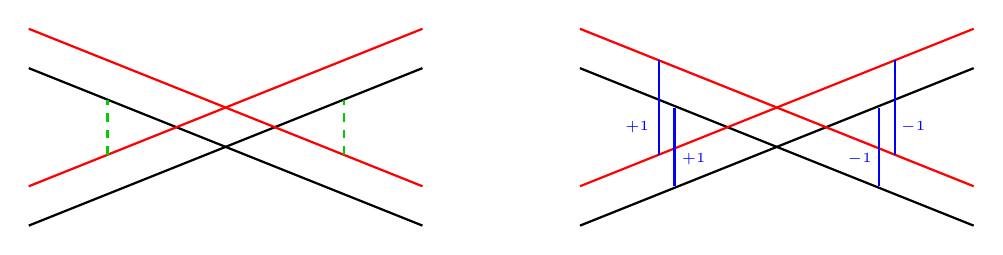
\begin{tikzpicture}%[scale=3]
\begin{scope} %left hand diagram with exchange points
\draw[thick] (-2.5,-1)--(2.5,1);
\draw[thick] (2.5,-1)--(-2.5,1);

\draw[thick,red] (-2.5,-.5)--(2.5,1.5);
\draw[thick,red] (2.5,-.5)--(-2.5,1.5);
\draw[dashed,green!80!black,thick] (-1.5,-.1)--(-1.5,.6) (1.5,-.1)--(1.5,.6);
\end{scope}
%
\begin{scope}[xshift=7cm] % right hand diagram with 4 handle-slides
\draw[thick] (-2.5,-1)--(2.5,1);
\draw[thick] (2.5,-1)--(-2.5,1);

\draw[thick,red] (-2.5,-.5)--(2.5,1.5);
\draw[thick,red] (2.5,-.5)--(-2.5,1.5);

\draw[blue,thick] (-1.5,-.1)--(-1.5,1.1) (1.5,-.1)--(1.5,1.1);
\draw[blue,thick] (-1.3,-.5)--(-1.3,0.5) (1.3,-.5)--(1.3,.5);
\draw[blue] (-1.5,0.25) node[left]{\tiny$+1$};
\draw[blue] (1.45,0.25) node[right]{\tiny$-1$};
\draw[blue] (-1.33,-.15) node[right]{\tiny$+1$};
\draw[blue] (1.33,-.15) node[left]{\tiny$-1$};
\end{scope}

\end{tikzpicture}
\caption{Each codimension-2 exchange stratum on the left, together with the red-to-black codimension-0 incident flows, forms two codimension-1 handle-slide strata on the right. Positive and negative handle-slide are mirror images since reversing the $x$-axis changes the signs of handle additions.We need to reverse the signs of these handle-slides in local nested case (3) of Figure \ref{fig: 3 cases of normal rulings}. See Figures \ref{fig: exchanges points give 6HS, dual}, \ref{fig: cancel black over red HS, dual}, \ref{fig: cancels HS, nested case,dual}.
}
\label{fig: exchanges points give 4HS}
\end{center}
\end{figure}
%
}

Recall from Figure \ref{fig: 3 cases of normal rulings} that the boundaries of the two $(n+1)$-manifolds can both be convex, or one can be convex and the other concave.
 For Case (1), nothing else needs to be done.
 Note that by Definition \ref{def: Ruling}.4, this is the only situation where one of the sheets involved in the switch might be an unpaired sheet (and so there is only one $(n+1)$-manifold).

In Case (2),  we need to introduce an additional exchange near, $({\pm 1} \times X) \times [\epsilon, 2\epsilon] \subset M \times \bR,$
as indicated in Figure \ref{fig: exchanges points give 6HS}.
%\footnote{\color{red}  Figures \ref{fig: exchanges points give 6HS} and \ref{fig: exchanges points give 6HS, dual} have $w$ and $-w$ indicated, and it's announced that the sign of $w$ is set later. Does this later sign-assignment reflect the new generalized definition of ruling? that is, that we are allowed to associate EITHER of the two adjacent $(n+1)$-manifolds to a switch, as long as the global $\bZ_2$-condition holds. It seems possible that we might end up with $w$ for both figures for this more generalized ruling, no?} 
We do so in a method similar to the two previously discussed exchanges.
Note here we explicitly use that both sheets involved with the switch are paired. 

{
%
\begin{figure}[htbp]
\begin{center}
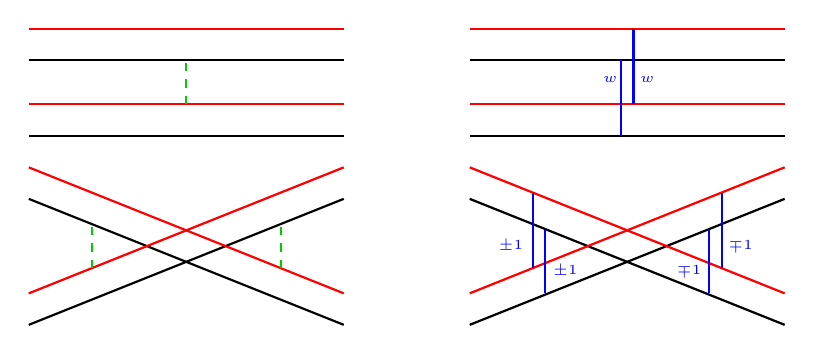
\begin{tikzpicture}[scale=.8]

\begin{scope}

\end{scope} 

\begin{scope} %left hand diagram with exchange points

\begin{scope}[yshift=12mm]
\draw[thick,red] (-2.5,2.5)--(2.5,2.5);
\draw[thick] (-2.5,2)--(2.5,2);
\end{scope}
\draw[thick,red] (-2.5,2.5)--(2.5,2.5);
\draw[thick] (-2.5,2)--(2.5,2);


\draw[thick] (-2.5,-1)--(2.5,1);
\draw[thick] (2.5,-1)--(-2.5,1);

\draw[thick,red] (-2.5,-.5)--(2.5,1.5);
\draw[thick,red] (2.5,-.5)--(-2.5,1.5);
\draw[dashed,green!80!black,thick] (-1.5,-.1)--(-1.5,.6) (1.5,-.1)--(1.5,.6) (0,2.5)--(0,3.2);
\end{scope}
%
\begin{scope}[xshift=7cm] % right hand diagram with 4 handle-slides
\draw[thick] (-2.5,-1)--(2.5,1);
\draw[thick] (2.5,-1)--(-2.5,1);

\draw[thick,red] (-2.5,-.5)--(2.5,1.5);
\draw[thick,red] (2.5,-.5)--(-2.5,1.5);

\draw[blue,thick] (-1.5,-.1)--(-1.5,1.1) (1.5,-.1)--(1.5,1.1);
\draw[blue,thick] (-1.3,-.5)--(-1.3,0.5) (1.3,-.5)--(1.3,.5);
\draw[blue] (-1.5,0.25) node[left]{\tiny$\pm1$};
\draw[blue] (1.45,0.25) node[right]{\tiny$\mp1$};
\draw[blue] (-1.33,-.15) node[right]{\tiny$\pm1$};
\draw[blue] (1.33,-.15) node[left]{\tiny$\mp1$};

\begin{scope}[yshift=12mm]
\draw[thick,red] (-2.5,2.5)--(2.5,2.5);
\draw[thick] (-2.5,2)--(2.5,2);
\end{scope}
\draw[thick,red] (-2.5,2.5)--(2.5,2.5);
\draw[thick] (-2.5,2)--(2.5,2);

\draw[thick,blue] (.1,2.5)--(.1,3.7);
\draw[thick,blue] (-.1,2)--(-.1,3.2);
\draw[blue] (.05,2.9) node[right]{\tiny$w$};
\draw[blue] (0,2.9) node[left]{\tiny$w$};
\end{scope}

\end{tikzpicture}
\caption{Additional exchange at nested pair of rulings gives a third pair of  handle-slides where $w \in \{-1,+1\}$ is a later local determination. To simplify the exposition, in subsequent figures we will just set $\pm 1 = 1, \mp 1 = -1.$}
\label{fig: exchanges points give 6HS}
\end{center}
\end{figure}
%
}

In Case (3), we use the inverted Figure \ref{fig: exchanges points give 6HS, dual} below.



{
%
\begin{figure}[htbp]
\begin{center}
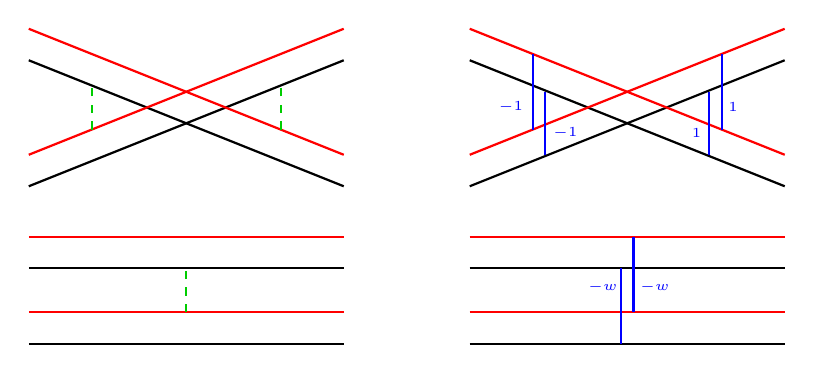
\begin{tikzpicture}[scale=.8]

\begin{scope}

\end{scope} 

\begin{scope} %left hand diagram with exchange points

\begin{scope}[yshift=-5.5cm]
\begin{scope}[yshift=12mm]
\draw[thick,red] (-2.5,2.5)--(2.5,2.5);
\draw[thick] (-2.5,2)--(2.5,2);
\end{scope}
\draw[thick,red] (-2.5,2.5)--(2.5,2.5);
\draw[thick] (-2.5,2)--(2.5,2);
\draw[dashed,green!80!black,thick] (0,2.5)--(0,3.2);
\end{scope}

\draw[thick] (-2.5,-1)--(2.5,1);
\draw[thick] (2.5,-1)--(-2.5,1);

\draw[thick,red] (-2.5,-.5)--(2.5,1.5);
\draw[thick,red] (2.5,-.5)--(-2.5,1.5);
\draw[dashed,green!80!black,thick] (-1.5,-.1)--(-1.5,.6) (1.5,-.1)--(1.5,.6);
\end{scope}
%
\begin{scope}[xshift=7cm] % right hand diagram with 4 handle-slides
\draw[thick] (-2.5,-1)--(2.5,1);
\draw[thick] (2.5,-1)--(-2.5,1);

\draw[thick,red] (-2.5,-.5)--(2.5,1.5);
\draw[thick,red] (2.5,-.5)--(-2.5,1.5);

\draw[blue,thick] (-1.5,-.1)--(-1.5,1.1) (1.5,-.1)--(1.5,1.1);
\draw[blue,thick] (-1.3,-.5)--(-1.3,0.5) (1.3,-.5)--(1.3,.5);
\draw[blue] (-1.5,0.25) node[left]{\tiny$-1$};
\draw[blue] (1.45,0.25) node[right]{\tiny$1$};
\draw[blue] (-1.33,-.15) node[right]{\tiny$-1$};
\draw[blue] (1.33,-.15) node[left]{\tiny$1$};

\begin{scope}[yshift=-5.5cm]
\begin{scope}[yshift=12mm]
\draw[thick,red] (-2.5,2.5)--(2.5,2.5);
\draw[thick] (-2.5,2)--(2.5,2);
\end{scope}
\draw[thick,red] (-2.5,2.5)--(2.5,2.5);
\draw[thick] (-2.5,2)--(2.5,2);

\draw[thick,blue] (.1,2.5)--(.1,3.7);
\draw[thick,blue] (-.1,2)--(-.1,3.2);
\draw[blue] (.05,2.9) node[right]{\tiny$-w$};
\draw[blue] (0,2.9) node[left]{\tiny$-w$};
\end{scope}
\end{scope}

\end{tikzpicture}
\caption{This is Figure \ref{fig: exchanges points give 6HS} inverted using the remark from (St1) that the dual of handle-slide $x_{ij}^u$ is $x_{ji}^{-u}$.}
\label{fig: exchanges points give 6HS, dual}
\end{center}
\end{figure}
%
}


% \begin{figure}
%\caption{The first two diagrams (reading from left) represent what to do when the switch corresponds to two manifolds convex boundaries. The vertical dotted lines in the leftmost diagram represent the first two exchange strata,  each  codimension-2 in basespace-time. Together with the codimension-0 incident flows shaded in the second (from left) diagram, these form the four families of codimension-1 handle-slides in the second diagram.
%The next two diagrams are for when the switch corresponds to convex and  concave boundaries. Here an additional family of exchanges are introduced, resulting in two additional families of handle-slides, similar to the first case.}
%\label{fig: CrossingExchanges}
%\end{figure}



\smallskip
 
  \noindent
 {\bf{Part 1c:}} Constructing the generating families when $2 \epsilon \le t \le T$ with $T >>1.$  
 
 \smallskip

The nearby Lagrangian hypothesis implies that there is a contact isotopy of $J^1 M$ inducing a Legendrian isotopy of the link $\Lambda \cup \Lambda_t$ for $\epsilon \le t \le T.$
For any sufficiently large $T >>1,$ all sheets of $\pi_F(\Lambda_T)$ lie above all sheets of $\pi_F(\Lambda).$
We construct the generating family for $\Lambda \cup \Lambda_t$ when $2\epsilon \le t \le T.$


%Assume we have stabilized for some sufficiently large $N,$ $f: (F \times \bR^K \rightarrow W \times \bR^N \rightarrow M) \rightarrow \bR.$ 

\color{red} 
We adapt the constructions in Milnor's Rearrangement Theorems \cite[Section 4]{M65} to our $\dim(M)$-parameter setting.
After possibly stabilizing, none of the fiber-critical points are local maxes or mins. So to each critical point representing $\Lambda_t,$ we can perform a ``finger-move" which raises its action value and which is supported in a small neighborhood of its descending manifold.
\color{black}
%Recall that we can assume each red-black pair of fiber critical points with non-zero incidence matrix entry, have non-zero coordinate-values on a unique $\bR^2$-factor of the fiber. So we can increase with $t$ the critical values of red fiber critical point by scaling the quadratic term associated to those coordinates.
%To finish the construction, over each cusp-locus, we match these increases in the correspond $\bR^4$-factor of the fiber (see Part 1a).
This has the effect of translating $\Lambda_t$ in the positive $z$-direction.
Here we are using a property justified later (but independently) in Part 1d. any handle-slides with upper sheet in $\Lambda$ and lower sheet in $\Lambda_t,$ where one of the sheets might not be related to the four sheets of the red and black cusp pairs, does not come close to these cusps; thus, the birth/deaths remain independent.

Note we can assume that the $M$-coordinates of the handles-slides with upper sheet in $\Lambda_t$ and lower sheet in $\Lambda$ from Figure \ref{fig: doubling L} remain  fixed as $t $ increases.

{\color{red} probably best to say they lie over the same point of $M$ as $t$ increases, ``coordinate" not clear}




%\color{red} [Do we need here some statement like ``Third, there are no flow lines that suddenly appear between un-paired sheets?"] \color{black}




% \begin{figure}
%
%\caption{The handle-slides are indicated as vertical lines. Note that these run between sheets of the same Maslov potential, assuming it is well-defined.}
%\label{fig: 2copyGF}
%\end{figure}
 
\smallskip
 
 \noindent
 {\bf{Part 1d:}} The handle-slides with upper sheet in $\Lambda$ and lower sheet in $\Lambda_t$
 \smallskip 
 
The handle-slides with upper sheet in $\Lambda$ and lower sheet in $\Lambda_t$ are ``forced" to move away from the cusp, due to the moving crossing of their upper and lower sheets. %See the right diagram of Figure \ref{fig: 2copyGF}. 
{\color{red} still suspicious about all these quotation marks, what does ``forced" actually mean?}
As long as these moving handle-slides are between consecutive sheets as measured in the $z$-direction, there are no Steinberg/exchange/similar relations, and so the manifold property of handle-slides ensures that they persist as $t$ increases.  
Consider the moment in spacetime when an intermediate third (red or black) sheet crosses one of the sheets.

If this third sheet's crossing it is not affiliated with a switch in the ruling, then the family of handle-slides continues through the crossing unchanged.
We can assume this because of the non-existence of fiberwise flow lines connecting this third sheet to the either of the two handle-slide's sheets.


 

Figure \ref{fig: cancel black over red HS} shows what happens to a handle-slide, ``forced" to move away from the cusps in Figure \ref{fig: doubling L},  when it approaches a switch, due to the  presence of the handle-slides created in 
Figure \ref{fig: exchanges points give 4HS}.
Note that here we use the switch is co-orientable in order to assume that the two $u$'s have the same sign in the leftmost diagram of Figure \ref{fig: exchanges points give 4HS}.
Figure \ref{fig: cancels HS, nested case} corresponds to 
Figure \ref{fig: exchanges points give 6HS}.
In particular, note the various (St3)-relations. 
From an equivalent viewpoint, Figure \ref{fig: cancel black over red HS} also shows that a handle-slide with sign $u$ on the left will slide across and change sign to produce $-u$ on the right as in Figure \ref{fig: cancel black over red HS, dual}.
\color{red} We note that this interaction of handle-slides was also studied when  $\dim(\Lambda)=1$
by Henry, when he introduces Morse Complex Sequences in S\=R-form, see Section 6e2 in \cite{Henry11}.
%IN CASE THIS GETS LEFT OUT OF BIBLIO: Henry, Michael Connections between Floer-type invariants and Morse-type invariants of Legendrian knots Pacific Journal of Mathematics 249 (2011) 77–133
\color{black}

%{\color{blue} The end result is that the sign of the black over red handle-slide will change when it crosses a switch crossing in an essential way (as either the nested pairing or the upper pairing as shown in red in Figure \ref{fig: 3 cases of normal rulings}). Thus these handle-slides will all cancel assuming that we take opposite signs on cusp sets which are separated by an odd number of essential switch crossings. Condition (6) in Definition \ref{def: Ruling} implies that the parity of the number of essential switch crossing separating cusp sets is well defined. So, it is possible to choose signs for cusp sets satisfying this condition.}

%\color{red}[There are probably be several things to add in this step

%\begin{enumerate}\item We need some elaboration about signs canceling due to framing of handle-slides. I don't think switch needs to be co-oriented for this. {\color{blue}We need co-orientable.}

%\item I did not use Figure \ref{Fig: pushing handle-slides between switch crossings}, but Kiyoshi's idea is to decompose the $(n+1)$-manifold into neighborhoods of the switches, and the components of said neighborhoods. Figure \ref{Fig: pushing handle-slides between switch crossings} deals with one such component. {\color{blue} I took out Figure \ref{Fig: pushing handle-slides between switch crossings}}


%\item There is also the blue text that was in Part 1a, but that I have moved to the ``storage" in Section 4.3.1. I believe one of these paragraphs discusses why the handle-slides can be made frmaed up to sign in the complement of the switches.\end{enumerate}]\color{black}

 {
%
\begin{figure}[htbp]
\begin{center}
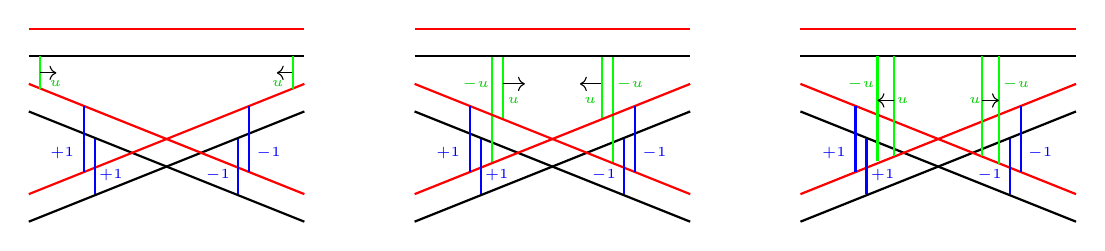
\begin{tikzpicture}[scale=.7]

\begin{scope}

\end{scope} 

\begin{scope} %left hand diagram with black/red pair to cancel
\draw[thick,red] (-2.5,2.5)--(2.5,2.5);
\draw[thick] (-2.5,2)--(2.5,2);

\draw[thick] (-2.5,-1)--(2.5,1);
\draw[thick] (2.5,-1)--(-2.5,1);

\draw[thick,red] (-2.5,-.5)--(2.5,1.5);
\draw[thick,red] (2.5,-.5)--(-2.5,1.5);

\draw[blue,thick] (-1.5,-.1)--(-1.5,1.1) (1.5,-.1)--(1.5,1.1);
\draw[blue,thick] (-1.3,-.5)--(-1.3,0.5) (1.3,-.5)--(1.3,.5);
\draw[blue] (-1.5,0.25) node[left]{\tiny$+1$};
\draw[blue] (1.45,0.25) node[right]{\tiny$-1$};
\draw[blue] (-1.4,-.15) node[right]{\tiny$+1$};
\draw[blue] (1.33,-.15) node[left]{\tiny$-1$};

\draw[green,thick] (-2.3,2)--(-2.3,1.4);
\draw[->] (-2.3,1.7)--(-2,1.7);
\draw[->] (2.3,1.7)--(2,1.7);
\draw[green,thick] (2.3,2)--(2.3,1.4);

\draw[green!80!black] (-2.3,1.5) node[right]{\tiny$u$};
\draw[green!80!black] (2.3,1.5) node[left]{\tiny$u$};

%\draw[dashed,green!80!black,thick] (-1.5,-.1)--(-1.5,.6) (1.5,-.1)--(1.5,.6);
\end{scope}
%
\begin{scope}[xshift=7cm] % middle diagram with 4 handle-slides
\draw[thick] (-2.5,-1)--(2.5,1);
\draw[thick] (2.5,-1)--(-2.5,1);

%\draw[green,thick] (2.3,2)--(2.3,1.4);
\draw[green,thick] (-1.1,2)--(-1.1,.04);
\draw[green,thick] (-.9,2)--(-.9,.85);
\draw[->] (-.9,1.5)--(-.5,1.5);
\draw[->] (.9,1.5)--(.5,1.5);
\draw[green!80!black] (-.97,1.5) node[left]{\tiny$-u$};
\draw[green!80!black] (-.99,1.2) node[right]{\tiny$u$};

\draw[green!80!black] (.97,1.2) node[left]{\tiny$u$};
\draw[green!80!black] (.99,1.5) node[right]{\tiny$-u$};

\draw[green,thick] (1.1,2)--(1.1,.04);
\draw[green,thick] (.9,2)--(.9,.85);


\draw[thick,red] (-2.5,-.5)--(2.5,1.5);
\draw[thick,red] (2.5,-.5)--(-2.5,1.5);

\draw[blue,thick] (-1.5,-.1)--(-1.5,1.1) (1.5,-.1)--(1.5,1.1);
\draw[blue,thick] (-1.3,-.5)--(-1.3,0.5) (1.3,-.5)--(1.3,.5);
\draw[blue] (-1.5,0.25) node[left]{\tiny$+1$};
\draw[blue] (1.45,0.25) node[right]{\tiny$-1$};
\draw[blue] (-1.4,-.15) node[right]{\tiny$+1$};
\draw[blue] (1.33,-.15) node[left]{\tiny$-1$};

\draw[thick,red] (-2.5,2.5)--(2.5,2.5);
\draw[thick] (-2.5,2)--(2.5,2);

%\draw[thick,blue] (.1,2.5)--(.1,3.7);
%\draw[thick,blue] (-.1,2)--(-.1,3.2);
\end{scope}
%%%

\begin{scope}[xshift=14cm] % right hand diagram with 4 handle-slides
\draw[thick] (-2.5,-1)--(2.5,1);
\draw[thick] (2.5,-1)--(-2.5,1);

\draw[thick,red] (-2.5,-.5)--(2.5,1.5);
\draw[thick,red] (2.5,-.5)--(-2.5,1.5);

\draw[blue,thick] (-1.5,-.1)--(-1.5,1.1) (1.5,-.1)--(1.5,1.1);
\draw[blue,thick] (-1.3,-.5)--(-1.3,0.5) (1.3,-.5)--(1.3,.5);
\draw[blue] (-1.5,0.25) node[left]{\tiny$+1$};
\draw[blue] (1.45,0.25) node[right]{\tiny$-1$};
\draw[blue] (-1.4,-.15) node[right]{\tiny$+1$};
\draw[blue] (1.33,-.15) node[left]{\tiny$-1$};

\draw[thick,red] (-2.5,2.5)--(2.5,2.5);
\draw[thick] (-2.5,2)--(2.5,2);

\draw[green,thick] (-1.1,2)--(-1.1,.1);
\draw[green,thick] (1.1,2)--(1.1,.04);

\draw[green,thick] (.8,2)--(.8,.2);
\draw[green,thick] (-.8,2)--(-.8,.2);
\draw[->] (.8,1.2)--(1.1,1.2);
\draw[->] (-.8,1.2)--(-1.1,1.2);

\draw[green!80!black] (-.98,1.5) node[left]{\tiny$-u$};
\draw[green!80!black] (-.93,1.2) node[right]{\tiny$u$};

\draw[green!80!black] (.95,1.2) node[left]{\tiny$u$};
\draw[green!80!black] (.99,1.5) node[right]{\tiny$-u$};

%\draw[thick,blue] (.1,2.5)--(.1,3.7);
%\draw[thick,blue] (-.1,2)--(-.1,3.2);
\end{scope}

\end{tikzpicture}
\caption{At a switch which is convex (or unpaired) on the bottom, we can cancel the unwanted black over red handle-slides. Each handle-slide, when pushed to the center, produces two handle-slides which cancel in pairs. There are two cases: $u=1$, $u=-1$.}
\label{fig: cancel black over red HS}
\end{center}
\end{figure}
%
}
 
 {
%
\begin{figure}[htbp]
\begin{center}
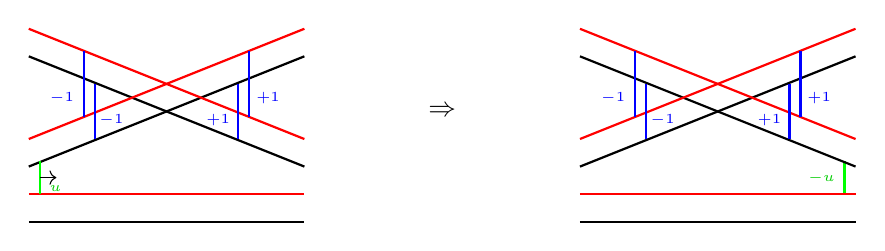
\begin{tikzpicture}[scale=.7]

\begin{scope}

\end{scope} 

\begin{scope} %left hand diagram with black/red pair to cancel
\begin{scope}[yshift=-4cm]
\draw[thick,red] (-2.5,2.5)--(2.5,2.5);
\draw[thick] (-2.5,2)--(2.5,2);
\end{scope}

\draw[thick] (-2.5,-1)--(2.5,1);
\draw[thick] (2.5,-1)--(-2.5,1);

\draw[thick,red] (-2.5,-.5)--(2.5,1.5);
\draw[thick,red] (2.5,-.5)--(-2.5,1.5);

\draw[blue,thick] (-1.5,-.1)--(-1.5,1.1) (1.5,-.1)--(1.5,1.1);
\draw[blue,thick] (-1.3,-.5)--(-1.3,0.5) (1.3,-.5)--(1.3,.5);
\draw[blue] (-1.5,0.25) node[left]{\tiny$-1$};
\draw[blue] (1.45,0.25) node[right]{\tiny$+1$};
\draw[blue] (-1.4,-.15) node[right]{\tiny$-1$};
\draw[blue] (1.33,-.15) node[left]{\tiny$+1$};

\begin{scope}[yshift=-2.9cm]
\draw[green,thick] (-2.3,2)--(-2.3,1.4);
\draw[->] (-2.3,1.7)--(-2,1.7);
%\draw[->] (2.3,1.7)--(2,1.7);
%\draw[green,thick] (2.3,2)--(2.3,1.4);

\draw[green!80!black] (-2.3,1.5) node[right]{\tiny$u$};
%\draw[green!80!black] (2.3,1.5) node[left]{\tiny$u$};

\end{scope}
%\draw[dashed,green!80!black,thick] (-1.5,-.1)--(-1.5,.6) (1.5,-.1)--(1.5,.6);
\end{scope}
%

\draw (5,0) node{$\Rightarrow$};

\begin{scope}[xshift=10cm] % right hand diagram with 4 handle-slides
\begin{scope}[yshift=-2.9cm]
%\draw[green,thick] (-2.3,2)--(-2.3,1.4);
%\draw[->] (-2.3,1.7)--(-2,1.7);
%\draw[->] (2.3,1.7)--(2,1.7);
\draw[green,thick] (2.3,2)--(2.3,1.4);

%\draw[green!80!black] (-2.3,1.5) node[right]{\tiny$u$};
\draw[green!80!black] (2.3,1.7) node[left]{\tiny$-u$};

\end{scope}


\begin{scope}[yshift=-4cm]

\draw[thick,red] (-2.5,2.5)--(2.5,2.5);
\draw[thick] (-2.5,2)--(2.5,2);
\end{scope}

\draw[thick] (-2.5,-1)--(2.5,1);
\draw[thick] (2.5,-1)--(-2.5,1);

\draw[thick,red] (-2.5,-.5)--(2.5,1.5);
\draw[thick,red] (2.5,-.5)--(-2.5,1.5);

\draw[blue,thick] (-1.5,-.1)--(-1.5,1.1) (1.5,-.1)--(1.5,1.1);
\draw[blue,thick] (-1.3,-.5)--(-1.3,0.5) (1.3,-.5)--(1.3,.5);
\draw[blue] (-1.5,0.25) node[left]{\tiny$-1$};
\draw[blue] (1.45,0.25) node[right]{\tiny$+1$};
\draw[blue] (-1.4,-.15) node[right]{\tiny$-1$};
\draw[blue] (1.33,-.15) node[left]{\tiny$+1$};

%\draw[green,thick] (-2.3,2)--(-2.3,1.4);
%\draw[->] (-2.3,1.7)--(-2,1.7);
%\draw[->] (2.3,1.7)--(2,1.7);
%\draw[green,thick] (2.3,2)--(2.3,1.4);

%\draw[green!80!black] (-2.3,1.5) node[right]{\tiny$u$};
%\draw[green!80!black] (2.3,1.5) node[left]{\tiny$u$};
%\draw[thick,blue] (.1,2.5)--(.1,3.7);
%\draw[thick,blue] (-.1,2)--(-.1,3.2);
\end{scope}

\end{tikzpicture}
\caption{At a switch which is convex (or unpaired) on the top of a pairing, we can move the unwanted black over red handle-slides from left to right, reversing its sign. This is the inversion of Figure \ref{fig: cancel black over red HS} in an equivalent formulation since moving $u$ on the left to $-u$ on the right is the same as cancelling $u$ on both sides}
\label{fig: cancel black over red HS, dual}
\end{center}
\end{figure}
%
}



{
%
\begin{figure}[htbp]%\label{fig: cancels HS, nested case}

\begin{center}
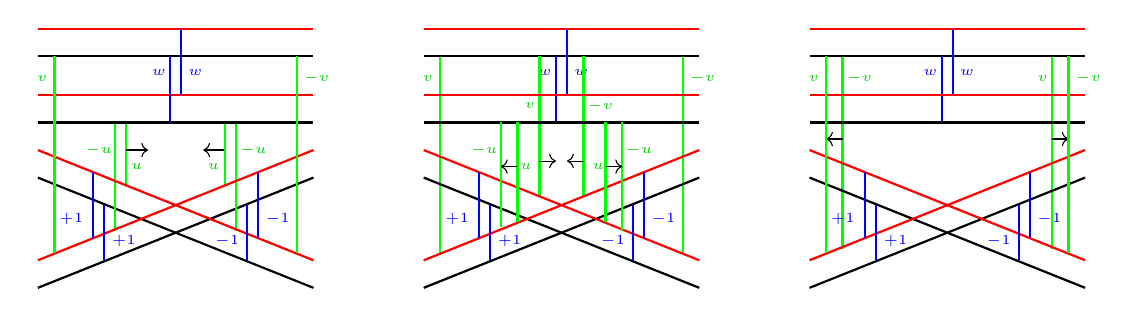
\begin{tikzpicture}[scale=.7]


\begin{scope}[xshift=21cm] %right hand diagram with black/red pair to cancel

\draw[thick,green] (-1.9,3.2)--(-1.9,-.3);
\draw[thick,green] (1.9,3.2)--(1.9,-.3);
\draw[->] (1.9,1.7)--(2.2,1.7);
\draw[->] (-1.9,1.7)--(-2.2,1.7);
\draw[blue] (-1.5,0.25) node[left]{\tiny$+1$};
\draw[blue] (1.45,0.25) node[right]{\tiny$-1$};
\draw[blue] (-1.33,-.15) node[right]{\tiny$+1$};
\draw[blue] (1.33,-.15) node[left]{\tiny$-1$};
\draw[blue] (.05,2.9) node[right]{\tiny$w$};
\draw[blue] (0,2.9) node[left]{\tiny$w$};

\draw[green!80!black] (-2.15,2.8)node[left]{\tiny$v$};
\draw[green!80!black] (2.15,2.8)node[right]{\tiny$-v$};

\draw[green!80!black] (-2,2.8)node[right]{\tiny$-v$};
\draw[green!80!black] (2,2.8)node[left]{\tiny$v$};

\begin{scope}[yshift=12mm]
\draw[thick,red] (-2.5,2.5)--(2.5,2.5);
\draw[thick] (-2.5,2)--(2.5,2);
\end{scope}
\draw[thick,blue] (.1,2.5)--(.1,3.7);
\draw[thick,blue] (-.1,2)--(-.1,3.2);

\draw[thick,red] (-2.5,2.5)--(2.5,2.5);
\draw[thick] (-2.5,2)--(2.5,2);

\draw[thick] (-2.5,-1)--(2.5,1);
\draw[thick] (2.5,-1)--(-2.5,1);

\draw[thick,red] (-2.5,-.5)--(2.5,1.5);
\draw[thick,red] (2.5,-.5)--(-2.5,1.5);

\draw[blue,thick] (-1.5,-.1)--(-1.5,1.1) (1.5,-.1)--(1.5,1.1);
\draw[blue,thick] (-1.3,-.5)--(-1.3,0.5) (1.3,-.5)--(1.3,.5);

%\draw[green,thick] (-2.3,2)--(-2.3,1.4);
%\draw[->] (-2.3,1.7)--(-2,1.7);
%\draw[->] (2.3,1.7)--(2,1.7);
%\draw[green,thick] (2.3,2)--(2.3,1.4);

\draw[thick,green] (-2.2,3.2)--(-2.2,-.37);
\draw[thick,green] (2.2,3.2)--(2.2,-.37);


%\draw[dashed,green!80!black,thick] (-1.5,-.1)--(-1.5,.6) (1.5,-.1)--(1.5,.6);
\end{scope}
%
\begin{scope}[xshift=7cm] % left hand diagram with 6 handle-slides
\draw[green!80!black] (-.97,1.5) node[left]{\tiny$-u$};
\draw[green!80!black] (-.99,1.2) node[right]{\tiny$u$};

\draw[green!80!black] (.97,1.2) node[left]{\tiny$u$};
\draw[green!80!black] (.99,1.5) node[right]{\tiny$-u$};

\draw[blue] (-1.5,0.25) node[left]{\tiny$+1$};
\draw[blue] (1.45,0.25) node[right]{\tiny$-1$};
\draw[blue] (-1.33,-.15) node[right]{\tiny$+1$};
\draw[blue] (1.33,-.15) node[left]{\tiny$-1$};
\draw[blue] (.05,2.9) node[right]{\tiny$w$};
\draw[blue] (0,2.9) node[left]{\tiny$w$};

\draw[green!80!black] (-2.15,2.8)node[left]{\tiny$v$};
\draw[green!80!black] (2.15,2.8)node[right]{\tiny$-v$};

\draw[thick] (-2.5,-1)--(2.5,1);
\draw[thick] (2.5,-1)--(-2.5,1);

%\draw[green,thick] (2.3,2)--(2.3,1.4);
\draw[green,thick] (-1.1,2)--(-1.1,.04);
\draw[green,thick] (-.9,2)--(-.9,.85);
\draw[->] (-.9,1.5)--(-.5,1.5);
\draw[->] (.9,1.5)--(.5,1.5);

\draw[green,thick] (1.1,2)--(1.1,.04);
\draw[green,thick] (.9,2)--(.9,.85);


\draw[thick,red] (-2.5,-.5)--(2.5,1.5);
\draw[thick,red] (2.5,-.5)--(-2.5,1.5);

\draw[blue,thick] (-1.5,-.1)--(-1.5,1.1) (1.5,-.1)--(1.5,1.1);
\draw[blue,thick] (-1.3,-.5)--(-1.3,0.5) (1.3,-.5)--(1.3,.5);

\draw[thick,red] (-2.5,2.5)--(2.5,2.5);
\draw[thick] (-2.5,2)--(2.5,2);

\begin{scope}[yshift=12mm]
\draw[thick,red] (-2.5,2.5)--(2.5,2.5);
\draw[thick] (-2.5,2)--(2.5,2);
\end{scope}
\draw[thick,blue] (.1,2.5)--(.1,3.7);
\draw[thick,blue] (-.1,2)--(-.1,3.2);

%\draw[thick,blue] (.1,2.5)--(.1,3.7);
%\draw[thick,blue] (-.1,2)--(-.1,3.2);

\draw[thick,green] (-2.2,3.2)--(-2.2,-.37);
\draw[thick,green] (2.2,3.2)--(2.2,-.37);

\end{scope}
%%%

\begin{scope}[xshift=14cm] % middle diagram with 6 handle-slides

\draw[blue] (-1.5,0.25) node[left]{\tiny$+1$};
\draw[blue] (1.45,0.25) node[right]{\tiny$-1$};
\draw[blue] (-1.33,-.15) node[right]{\tiny$+1$};
\draw[blue] (1.33,-.15) node[left]{\tiny$-1$};
\draw[blue] (.05,2.9) node[right]{\tiny$w$};
\draw[blue] (0,2.9) node[left]{\tiny$w$};
\draw[green!80!black] (-.3,2.3)node[left]{\tiny$v$};
\draw[green!80!black] (.3,2.3)node[right]{\tiny$-v$};


\draw[green!80!black] (-2.15,2.8)node[left]{\tiny$v$};
\draw[green!80!black] (2.15,2.8)node[right]{\tiny$-v$};

\draw[green!80!black] (-.98,1.5) node[left]{\tiny$-u$};
\draw[green!80!black] (-.93,1.2) node[right]{\tiny$u$};

\draw[green!80!black] (.95,1.2) node[left]{\tiny$u$};
\draw[green!80!black] (.99,1.5) node[right]{\tiny$-u$};


\draw[thick,green] (-2.2,3.2)--(-2.2,-.37);
\draw[thick,green] (2.2,3.2)--(2.2,-.37);

\begin{scope}[yshift=12mm]
\draw[thick,red] (-2.5,2.5)--(2.5,2.5);
\draw[thick] (-2.5,2)--(2.5,2);
\end{scope}
\draw[thick,blue] (.1,2.5)--(.1,3.7);
\draw[thick,blue] (-.1,2)--(-.1,3.2);

\draw[green,thick] (-.4,3.2)--(-.4,.65);
\draw[green,thick] (.4,3.2)--(.4,.65);
\draw[->] (-.4,1.3)--(-.1,1.3);
\draw[->] (.4,1.3)--(.1,1.3);

\draw[thick] (-2.5,-1)--(2.5,1);
\draw[thick] (2.5,-1)--(-2.5,1);

\draw[thick,red] (-2.5,-.5)--(2.5,1.5);
\draw[thick,red] (2.5,-.5)--(-2.5,1.5);

\draw[blue,thick] (-1.5,-.1)--(-1.5,1.1) (1.5,-.1)--(1.5,1.1);
\draw[blue,thick] (-1.3,-.5)--(-1.3,0.5) (1.3,-.5)--(1.3,.5);

\draw[thick,red] (-2.5,2.5)--(2.5,2.5);
\draw[thick] (-2.5,2)--(2.5,2);

\draw[green,thick] (-1.1,2)--(-1.1,.1);
\draw[green,thick] (1.1,2)--(1.1,.04);

\draw[green,thick] (.8,2)--(.8,.2);
\draw[green,thick] (-.8,2)--(-.8,.2);
\draw[->] (.8,1.2)--(1.1,1.2);
\draw[->] (-.8,1.2)--(-1.1,1.2);
%\draw[thick,blue] (.1,2.5)--(.1,3.7);
%\draw[thick,blue] (-.1,2)--(-.1,3.2);
\end{scope}

\end{tikzpicture}
\caption{At a nested switch we first cancel the inner black/red handle-slides with signs $u,u$. This produces new handle-slides which cancel the outer black/red handle-slides. These long handle-slides need to have signs $v,-v$, as shown, in order to cancel in the middle, assuming that $uw=v$.}
\label{fig: cancels HS, nested case}
\end{center}
\end{figure}
%
}

{
%
\begin{figure}[htbp]%\label{fig: cancels HS, nested case}

\begin{center}
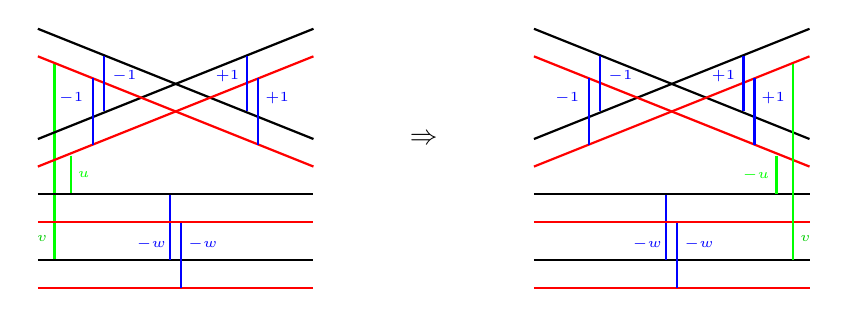
\begin{tikzpicture}[scale=.7,yscale=-1]

\draw (11.5,1) node{$\Rightarrow$};

\begin{scope}[xshift=16cm] %right hand diagram with black/red pair to cancel

\draw[blue] (-1.5,0.25) node[left]{\tiny$-1$};
\draw[blue] (1.45,0.25) node[right]{\tiny$+1$};
\draw[blue] (-1.33,-.15) node[right]{\tiny$-1$};
\draw[blue] (1.33,-.15) node[left]{\tiny$+1$};
\draw[blue] (.05,2.9) node[right]{\tiny$-w$};
\draw[blue] (0,2.9) node[left]{\tiny$-w$};


\begin{scope}[yshift=12mm]
\draw[thick,red] (-2.5,2.5)--(2.5,2.5);
\draw[thick] (-2.5,2)--(2.5,2);
\end{scope}
\draw[thick,blue] (.1,2.5)--(.1,3.7);
\draw[thick,blue] (-.1,2)--(-.1,3.2);

\draw[thick,red] (-2.5,2.5)--(2.5,2.5);
\draw[thick] (-2.5,2)--(2.5,2);

\draw[thick] (-2.5,-1)--(2.5,1);
\draw[thick] (2.5,-1)--(-2.5,1);

\draw[thick,red] (-2.5,-.5)--(2.5,1.5);
\draw[thick,red] (2.5,-.5)--(-2.5,1.5);

\draw[blue,thick] (-1.5,-.1)--(-1.5,1.1) (1.5,-.1)--(1.5,1.1);
\draw[blue,thick] (-1.3,-.5)--(-1.3,0.5) (1.3,-.5)--(1.3,.5);

%\draw[green,thick] (-2.3,2)--(-2.3,1.4);
%\draw[->] (-2.3,1.7)--(-2,1.7);
%\draw[->] (2.3,1.7)--(2,1.7);
%\draw[green,thick] (2.3,2)--(2.3,1.4);

\draw[thick,green] (2.2,3.2)--(2.2,-.37);
\draw[thick,green] (1.9,1.3)--(1.9,2);
\draw[green] (1.95,1.65)node[left]{\tiny$-u$};
\draw[green!80!black] (2.15,2.8)node[right]{\tiny$v$};

\end{scope}
%


\begin{scope}[xshift=7cm] % left hand diagram with 6 handle-slides


\draw[thick,green] (-2.2,3.2)--(-2.2,-.37);

\draw[thick,green] (-1.9,1.3)--(-1.9,2);
%\draw[thick,green] (1.9,3.2)--(1.9,-.3);
\draw[green] (-1.95,1.65)node[right]{\tiny$u$};
%\draw[->] (1.9,1.7)--(2.2,1.7);
%\draw[->] (-1.9,1.7)--(-2.2,1.7);
\draw[blue] (-1.5,0.25) node[left]{\tiny$-1$};
\draw[blue] (1.45,0.25) node[right]{\tiny$+1$};
\draw[blue] (-1.33,-.15) node[right]{\tiny$-1$};
\draw[blue] (1.33,-.15) node[left]{\tiny$+1$};
\draw[blue] (.05,2.9) node[right]{\tiny$-w$};
\draw[blue] (0,2.9) node[left]{\tiny$-w$};

\draw[green!80!black] (-2.15,2.8)node[left]{\tiny$v$};

%\draw[green!80!black] (-2,2.8)node[right]{\tiny$-v$};
%\draw[green!80!black] (2,2.8)node[left]{\tiny$v$};

\begin{scope}[yshift=12mm]
\draw[thick,red] (-2.5,2.5)--(2.5,2.5);
\draw[thick] (-2.5,2)--(2.5,2);
\end{scope}
\draw[thick,blue] (.1,2.5)--(.1,3.7);
\draw[thick,blue] (-.1,2)--(-.1,3.2);

\draw[thick,red] (-2.5,2.5)--(2.5,2.5);
\draw[thick] (-2.5,2)--(2.5,2);

\draw[thick] (-2.5,-1)--(2.5,1);
\draw[thick] (2.5,-1)--(-2.5,1);

\draw[thick,red] (-2.5,-.5)--(2.5,1.5);
\draw[thick,red] (2.5,-.5)--(-2.5,1.5);

\draw[blue,thick] (-1.5,-.1)--(-1.5,1.1) (1.5,-.1)--(1.5,1.1);
\draw[blue,thick] (-1.3,-.5)--(-1.3,0.5) (1.3,-.5)--(1.3,.5);

%\draw[green,thick] (-2.3,2)--(-2.3,1.4);
%\draw[->] (-2.3,1.7)--(-2,1.7);
%\draw[->] (2.3,1.7)--(2,1.7);
%\draw[green,thick] (2.3,2)--(2.3,1.4);
\end{scope}
%%%


\end{tikzpicture}
\caption{At a downward convex nested switch we can slide the inner black/red handle-slides with signs $u$ and the long handle-slides have signs $v$ from left to right to obtain handle-slides $-u$ and $v$ on the right provided that $uw=v$. This is the inversion of Figure \ref{fig: cancels HS, nested case} from an equivalent perspective. For example, moving $u$ on the left to $-u$ on the right is the same as cancelling $u$ on both sides as in Figure \ref{fig: cancels HS, nested case}.
}
\label{fig: cancels HS, nested case,dual}
\end{center}
\end{figure}
%
}


 
%\begin{figure}
%\caption{Although this figure seems to illustrate (when $\dim(\Lambda) =1$) a handle-slide entering from the left and leaving on the right in a ``switched form", it actually represents how the boundaries of two handle-slide loci, each with upper sheet in $\Lambda$ and lower sheet in $\Lambda_t,$ can be identified.}
%\label{fig: HandleSlideSwitch}
%\end{figure}
%
%\begin{figure}
%\caption{The more complicated case from Figure \ref{fig: CrossingExchanges}.}
%\label{fig: HandleSlideSwitch2}
%\end{figure}

 \smallskip

  \noindent
 {\bf{Part 2:}} Computing a vanishing torsion at $t=T.$
 
 \smallskip



Part 1 produces generating families, framed up to sign, for an isotopy of the Legendrian unlink 
$\Lambda \cup \Lambda_t.$ 
As mentioned in Part 0, for sufficiently large $T$ (such that $\min z(\Lambda_T) >> \max z(\Lambda)$) we can compute the torsion of $\Lambda$ by looking at our generating family for $\Lambda \cup \Lambda_T$ restricted to $\Lambda.$ 
Note that the fiber of this restriction is no longer $\bR^N,$ but rather takes values in a tube. To see this, consider the fiber over one point $m\in M$, we can deform the single function $f_m$ so that it has exactly one critical point. That makes the fiber a tube. {\color{red} we need to be careful as we have already defined tube to be something else. the tube here is closer to the sense of Waldhausen. we need to quote \cite{ACGK}. then possibly \cite{AACK} to turn it into our version of tube}

So we have tube bundle supporting the generating family for $\Lambda$.
In Part 1, the generating family and its handle-slides are fully understood for $\Lambda \cup \Lambda_t$ when $ t \le 2 \epsilon,$ but only some of the handle-slides are discussed when $t > 2 \epsilon.$
In Part 2, we first complete the diagnosis of handle-slides when $2 \epsilon < t \le T$ by studying what possible (St3) relations involving the (known) pre-existing handle-slides can or cannot occur.
We then verify that handle-slides of the generating family for $\Lambda \cup \Lambda_T$ restricted to $\Lambda,$ contribute to vanishing torsion.


\smallskip


  \noindent
 {\bf{Part 2a:}} A correspondence between the moving handle-slides and the $(n+1)$-manifolds of the ruling.
 
 \smallskip


Consider the black-over-red moving handle-slides $x_{ij}^u$ first introduced in Figure \ref{fig: doubling L} and later studied in Figures \ref{fig: cancel black over red HS}, \ref{fig: cancel black over red HS, dual}, \ref{fig: cancels HS, nested case} and \ref{fig: cancels HS, nested case,dual}.
In our figures we have been identifying each one as a vertical line segment in $J^0(M).$
Extend each such segment so that it terminates on the black point of $\Lambda$ directly below its original red endpoint in $\Lambda_t.$
Then by our construction of exchanges in Part 1, the union of extended segments approximately {\color{red} what do you mean approximately?} traces out the immersed $(n+1)$-manifolds of the ruling. (Here the approximation ignores some ``reduncancy" of canceling segments as illustrated in the left-most diagrams of  Figures \ref{fig: cancel black over red HS} and \ref{fig: cancels HS, nested case}, as well as a small neighborhood of the cusps.)  {\color{red} ok I guess...}That the line segments coherently fit together to form a manifold follows from the Part 1 discussion of framings (up to sign) of these handle-slides;
see Figure \ref{Fig: black over red handle-slide sign pattern}.
The (possibly immersed) manifold property implies that these handles-slides disappear before $t=T,$ without relying on (St3)-relations, exchanges or other higher-codimension events, that
might then need to be calatogued for the torsion computation.

{
%
\begin{figure}[htbp]
\begin{center}
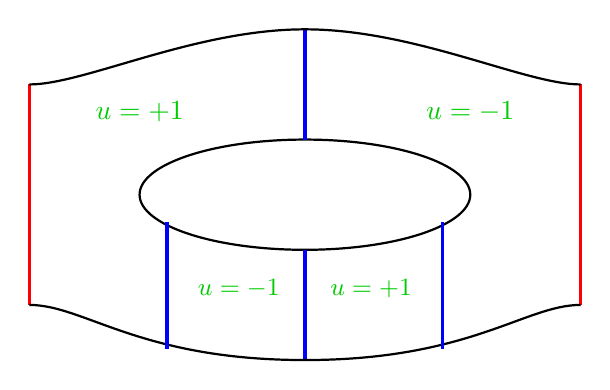
\begin{tikzpicture}[scale=.7]
\draw[very thick, red] (-5,-2)--(-5,2) (5,-2)--(5,2);
\draw[thick]  (0,0) ellipse[x radius=3cm, y radius=1cm];
\draw[very thick, blue] (0,1)--(0,3) (0,-1)--(0,-3);
\draw[thick] (-5,2) ..controls (-4,2) and (-2,3)..(0,3);
\draw[thick] (5,2) ..controls (4,2) and (2,3)..(0,3);
\draw[thick] (-5,-2) ..controls (-4,-2) and (-3,-3)..(0,-3);
\draw[thick] (5,-2) ..controls (4,-2) and (3,-3)..(0,-3);
\draw[very thick, blue] (-2.5,-.5)--(-2.5,-2.8)(2.5,-.5)--(2.5,-2.8);%  (0,-1)--(0,-3);
\draw[green!80!black] (-3,1.5) node{$u=+1$};
\draw[green!80!black] (3,1.5) node{$u=-1$};
\draw[green!80!black] (-1.2,-1.7) node{\small$u=-1$};
\draw[green!80!black] (1.2,-1.7) node{\small$u=+1$};
\end{tikzpicture}
\caption{When the black-over-red handle-slide produced at a cusp set (red) move across an essential switch crossing (blue), it changes sign. This figure shows a possible pattern of signs in one components of the manifold of pairing of a ruling. The sign pattern is well-defined since any closed curve gives an even number of sign switches by Definition \ref{def: Ruling}(6).}
\label{Fig: black over red handle-slide sign pattern}
\end{center}
\end{figure}
%
}

 \smallskip
%
%  \noindent
% {\bf{Part 2b:}} Completing the torsion calculation in the absence of other (St3)-relations.
% 
% \smallskip
% 
%\color{red} 
%If we assume that $\Lambda$ and $\Lambda_T$ are sufficiently far apart in the vertical direction, we can compute the torsion of $\Lambda$ by looking at our generating family for $\Lambda \cup \Lambda_T$ restricted to $\Lambda.$ 
%[Alternatively: we can argue that the torsion has a upper-block triangular form with identical entries in red-red and black-black submatrices.]
%Since our generating family is a framed family of Morse functions, it suffices to show that  Corollary \ref{cor: NoCodim4} applies to the generating family restricted to $\Lambda.$
%\color{black}
%So the remainder of the proof is to determine what (St3) relations (and higher codimension events) occurred between $t = \epsilon$ and $t = T.$
%
% \smallskip

  \noindent
 {\bf{Part 2b:}} The list of possible (St3)-relations to consider for $t \le T.$
 
 \smallskip

Let us label as the types of {\em{a priori}} known handle-slides as follows: (1rb) are the ones in Figure
\ref{fig: doubling L}  with red sheet on top and black on bottom, fixed in time;
(2br) are the ones in Figure
\ref{fig: doubling L}  with black sheet on top and red on bottom, varying in time; 
(3bb), resp. (3rr), are the ones in Figure \ref{fig: exchanges points give 4HS} with black, resp. red, sheets on top and bottom;
(4bb), resp. (4rr), are the ones in Figure \ref{fig: exchanges points give 6HS} but not in Figure \ref{fig: exchanges points give 4HS} with black, resp. red, sheets on top and bottom.
One obvious constraint is that if type ($nxy$) forms an (St3)-relation with type ($mwz$) for $n,m \in \{1,2,3,4\}$ and $x,y,w,z \in \{\mbox{r,b}\},$ then either $y=w$ or $x=z.$

Note that if an (St3)-relation involving a pair of the above handle-slides were to occur, this might create a new type of handle-slide, creating more possible (St3)-relations to consider.

 \smallskip

  \noindent
 {\bf{Part 2c:}} The easier eliminations of (St3)-relations.
 
 \smallskip

Type (1rb) cannot produce an (St3) with (2br),  (3bb), (3rr), (4bb) or (4rr) because such an (St3)  would contradict the pairing of sheets provided by the ruling. More specifically, at (1rb) both paired sheets cusp, which does not hold at the others. Here we use that a switch cannot intersect a cusp by the manifold property of any switch locus.

The contradiction in the pairing of sheets also eliminates an (St3) produced by (2br) and   (4rr).

Definition \ref{def: Ruling} stipulates that the base projections of two switches associated to the same  $(n+1)$-manifold do not intersect. The ruling's pairing thus eliminates an (St3) relation produced by:  (2br) and (3bb); (3rr) and (4rr); (3bb) and (4bb); (4rr) with itself; (4bb) with itself.

Figures \ref{fig: cancel black over red HS} and \ref{fig: cancels HS, nested case} handle all the (St3) relations produced by (2br) with either (3rr) or (4bb), and show no new types of handle-slides need to be considered.














%If there are no (St3) relations other than the ones in Figures and \ref{fig: cancel HS: convex case} and \ref{fig: cancels HS, nested case}, we claim the proof is complete.
%To see this claim, note that the moving handle-slides in Figure \ref{fig: doubling L}, when viewed as moving vertical lines, trace out the $(n+1)$-manifolds from Definition \ref{def: Ruling}. 
%(Here we make two identifications: the one discussed in the Figure \ref{fig: HandleSlideSwitch} caption; and the set of points in $\Lambda_t$ at the lower ends of these handle-slides with the corresponding set of points in $\Lambda.$)
%\color{red} [Maybe put in here Kiyoshi's description of drilling out the manifold around the crossings, to reduce the hard previous computations to local ones?] \color{black}
%The (possibly immersed) manifold property implies that these handles-slides disappear before $t=N,$ without relying on (St3)-relations, exchanges or other higher-codimension events, that
%would then need to be recorded for the torsion computation.
%%since all sheets of $\Lambda$ sit below the sheets of $\Lambda_N,$ where are no more such handles-slides.
%Both the handle-slides with upper sheet $\Lambda_t$ and lower sheet $\Lambda$ (see Figure \ref{fig: doubling L}) and the handle-slides whose two sheets lie on the same component of the link (see Figure \ref{fig: CrossingExchanges}) do not move with $t.$
%So if there are no (St3) relations, there are no contributions to the torsion of $\Lambda,$ as described in Lemma \ref{lem: NoCodim4}.
%This completes the proof of the claim.

%Suppose now there are some (St3)-relations aside from the ones in Figures \ref{fig: HandleSlideSwitch} and/or \ref{fig: HandleSlideSwitch2}. 
%We will derive a contradiction to the existence of a ruling.
%Any such (St3)-relation must involve the (fixed in $t$) handle-slides from Figures \ref{fig: doubling L} and/or \ref{fig: CrossingExchanges}.
%
%First consider an (St3)-relation involving a handle-slide from each of these two figures. This implies that a crossing of sheets $S_i,S_j$ affiliated with a switch intersects a cusp of sheets $S_j,S_k.$
%(The sheets are listed in no particular order.) But the boundary of the crossing locus at the cusp locus contradicts the manifold property of either of the two $(n+1)$-manifolds associated with this switch. In addition, a pairing cannot pair a cusping sheet to a third sheet not involved with the cusp, per Definition \ref{def: Ruling}.
%
%There are no (St3)-relations involving two (fixed in $t$) handle-slides from Figures \ref{fig: doubling L}, because the upper sheet of one (in $\Lambda_t$) cannot be the lower one in the other (in $\Lambda$). For a similar reason, there are no (St3)-relations involving two handle-slides of type Figures \ref{fig: HandleSlideSwitch} and  \ref{fig: HandleSlideSwitch2} where one is between two sheets of $\Lambda$ and the other between two sheets of $\Lambda_t.$


\smallskip

  \noindent
 {\bf{Part 2d:}} Eliminating (St3)-relations near three intersecting sheets.
 
 \smallskip

It remains to find all (St3) relations produced by (3bb) and (3bb). The (3rr) case is identical. We will show below that there are none. 

%So it remains to eliminate an (St3)-relation involving two handle-slides of type Figures \ref{fig: HandleSlideSwitch} or \ref{fig: HandleSlideSwitch2}, all of whose sheets lie in $\Lambda.$ The case $\Lambda_t$ is identical.
%To eliminate the handle-slides unique to Figure \ref{fig: HandleSlideSwitch2}, recall from in Definition \ref{def: Ruling} that a sheet away from a switch cannot be used in two pairings.
%So consider the handle-slides present in both figures.
For concreteness, assume the two handle-slides of type (3bb) have (top,bottom) sheets $(S_1,S_2)$ and $(S_2,S_3)$ of $\Lambda.$ 
%The (St3)-relation implies a handle-slide with (top,bottom) sheets $(S_1,S_3)$ appears. 
%Moreover, since the handle-slides are close to the $(S_1,S_2)$- and $(S_2,S_3)$-crossing loci, the (St3) relation is close to a (at most) codimension-2 triple crossing involving the three sheets. This is illustrated in the left and center diagrams of Figure \ref{fig: St3} \color{red} 5 \color{black}.
Since the handle-slides are close to the $(S_1,S_2)$- and $(S_2,S_3)$-crossing strata, the (St3) relation is close to a codimension-2 triple crossing involving the three sheets.
The first case (illustrated in the left diagram of Figure \ref{fig: St3})
is when the $(S_1,S_2)$- and $(S_2,S_3)$-crossing strata are the two top triangle-vertices.
The $(n+1)$-manifold whose boundary includes the upper blue curve, has a boundary with a codimension-2 stratum at the triple point, contradicting Definition \ref{def: Ruling}.
The second case (not illustrated) is when either  the $(S_1,S_2)$- or $(S_2,S_3)$-crossing strata is the bottom triangle-vertex.
Similar to the first case, the $(n+1)$-manifold whose boundary switches at this bottom vertex has a boundary with codimension-2 stratum.






   
 \begin{figure}
 {
\begin{center}
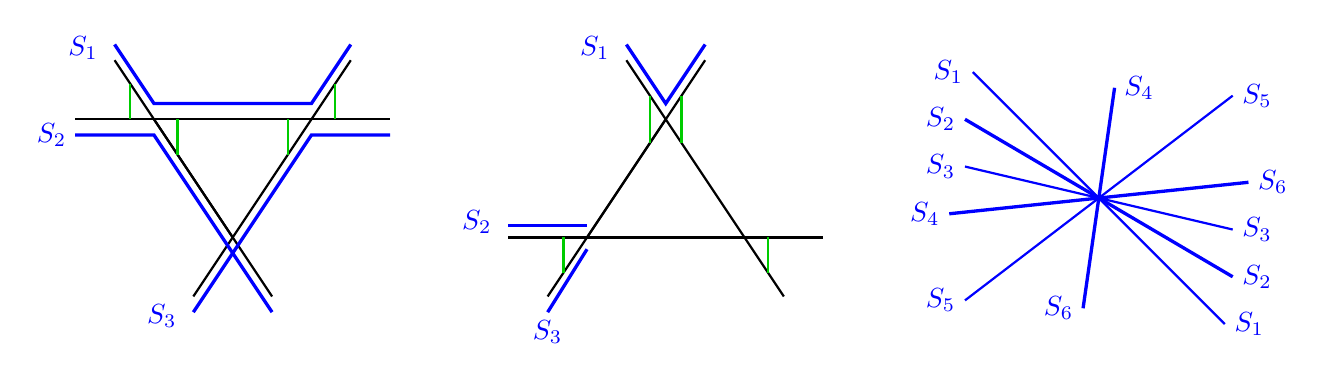
\begin{tikzpicture}%[scale=3]
{
\begin{scope}
\coordinate (C) at (0,.4);

\coordinate (A) at (0,-.5);
\coordinate (B1) at (-2,1);
\coordinate (B2) at (-1,1);
\coordinate (B3) at (1,1);
\coordinate (B4) at (2,1);
\coordinate (C1) at (-.5,-1.25);
\coordinate (C2) at (.5,-1.25);
\coordinate (A1) at (-1.5,1.75);
\coordinate (A2) at (1.5,1.75);
\coordinate (C0) at (0,-.5);
\coordinate (D1) at (-1,-.2);
\coordinate (D2) at (1,-.2);
\coordinate (D0) at (0,1.5);

%\draw (B3)--(D1) (B2)--(D2) (C0)--(D0);
\draw[fill,white] (B2)--(B3)--(C0);

\draw[thick] (B1)--(B4);
\draw[thick](B2)--(A)--(C1)--(A2);
\draw[thick](A1)--(C2);
%\draw (B2)--(C)--(B3) (C)--(C0);
%\draw[thick] (B1)--(D1)--(C1) (B4)--(D2)--(C2);
\begin{scope}[yshift=-2mm]
\draw[very thick,blue] (-2,1)--(-1,1)--(.5,-1.25);
\draw[very thick,blue] (2,1)--(1,1)--(-.5,-1.25);
\end{scope}
\begin{scope}[yshift=2mm]
\draw[very thick,blue] (-1.5,1.75)--(-1,1)--(1,1)--(1.5,1.75);
\end{scope}
\draw[thick,green!80!black] (-1.3,1)--(-1.3,1.45);
\draw[thick,green!80!black] (1.3,1)--(1.3,1.45);
\draw[thick,green!80!black] (-.7,1)--(-.7,.55);
\draw[thick,green!80!black] (.7,1)--(.7,.55);

\draw[blue] (-2.3,.8) node{$S_2$};
\draw[blue] (-1.9,1.9) node{$S_1$};
\draw[blue] (-.9,-1.5) node{$S_3$};
\end{scope}
}
{
\begin{scope}[xshift=5.5cm,yshift=5mm]
\coordinate (C) at (0,-.4);

\coordinate (A) at (0,.5);
\coordinate (B1) at (-2,-1);
\coordinate (B2) at (-1,-1);
\coordinate (B3) at (1,-1);
\coordinate (B4) at (2,-1);
\coordinate (C1) at (-.5,1.25);
\coordinate (C2) at (.5,1.25);
\coordinate (A1) at (-1.5,-1.75);
\coordinate (A2) at (1.5,-1.75);
\coordinate (C0) at (0,.5);
\coordinate (D1) at (-1,.2);
\coordinate (D2) at (1,.2);
\coordinate (D0) at (0,-1.5);

%\draw (B3)--(D1) (B2)--(D2) (C0)--(D0);
\draw[fill,white] (B2)--(B3)--(C0);

\draw[thick] (B1)--(B4);
\draw[thick](B2)--(A)--(C1)--(A2);
\draw[thick](A1)--(C2);
%\draw (B2)--(C)--(B3) (C)--(C0);
%\draw[thick] (B1)--(D1)--(C1) (B4)--(D2)--(C2) (A1)--(D0)--(A2);
%\draw[thick] (B1)--(D1)--(C1) (B4)--(D2)--(C2);
\draw[thick,green!80!black] (-1.3,-1)--(-1.3,-1.45);
\draw[thick,green!80!black] (1.3,-1)--(1.3,-1.45);
%\draw[thick,green!80!black] (-.7,-1)--(-.7,-.55);
%\draw[thick,green!80!black] (.7,-1)--(.7,-.55);
\draw[thick,green!80!black] (.2,.2)--(.2,.8);
\draw[thick,green!80!black] (-.2,.2)--(-.2,.8);

\draw[very thick,blue] (-.5,1.45) --( 0,.7)--(.5,1.45);

\draw[very thick,blue] (-2,-.85)--(-1,-.85);% --( 0,.3)--(1,-.85)--(2,-.85);
\draw[very thick,blue] (-1.5,-1.95)--(-1,-1.15);% --(1,-1.15)--(1.5,-1.95);
\draw[blue] (-2.4,-.8) node{$S_2$};
\draw[blue] (-.9,1.4) node{$S_1$};
\draw[blue] (-1.5,-2.2) node{$S_3$};

\end{scope}

\begin{scope}[xshift=11cm]%,yshift=5mm]
\coordinate (S1) at (-1.6,1.6);
\coordinate (S1p) at (1.6,-1.6);

\coordinate (S2) at (-1.7,1);
\coordinate (S2p) at  (1.7,-1);

\coordinate (S3) at (-1.7,.4);
\coordinate (S3p) at  (1.7,-.4);
\coordinate (S5) at (-1.7,-1.3);
\coordinate (S5p) at  (1.7,1.3);

\coordinate (S6) at (-.2,-1.4);
\coordinate (S6p) at  (.2,1.4);

\coordinate (S4) at (-1.9,-.2);
\coordinate (S4p) at  (1.9,.2);

\draw[very thick,blue] (S6)--(0,0)--(S6p);
\draw[blue] (S6)node[left]{$S_6$};
\draw[blue] (S6p)node[right]{$S_4$};

\draw[thick,blue] (S1)--(S1p);
\draw[blue] (S1)node[left]{$S_1$};
\draw[blue] (S1p)node[right]{$S_1$};
\draw[very thick,blue] (S2)--(S2p);
\draw[blue] (S2)node[left]{$S_2$};
\draw[blue] (S2p)node[right]{$S_2$};
\draw[thick,blue] (S3)--(S3p);
\draw[blue] (S3)node[left]{$S_3$};
\draw[blue] (S3p)node[right]{$S_3$};
\draw[very thick,blue] (S4)--(0,0)--(S4p);
\draw[blue] (S4)node[left]{$S_4$};
\draw[blue] (S4p)node[right]{$S_6$};
\draw[thick,blue] (S5)--(S5p);
\draw[blue] (S5)node[left]{$S_5$};
\draw[blue] (S5p)node[right]{$S_5$};
\end{scope}
}
\end{tikzpicture}
\end{center}
%
}
\caption{The upper  $(n+1)$-manifold with boundary drawn in blue fails the manifold condition in Definition \ref{def: Ruling}. Note only the boundary is specified, while the actual associated $(n+1)$-manifold might lie above or below it. %On the right is a crossing of 6 sheets which satisfies Definition \ref{def: Ruling}. This drawing suggests that only sheets $S_4$ and $S_6$ switch. No other sheet can switch with $S_4$ or $S_6$ without those 3 sheets producing a forbidden configuration as on the left.
}
\label{fig: St3}
\end{figure}


A priori, it is possible that the (St3)-relation occurs in a small neighborhood of a high-codimension singularity, as illustrated in the right diagram of Figure \ref{fig: St3}.
%[Current version of Figure \ref{fig: St3} does not have this high codim diagram.] \color{black}
But then well-known stratification theory  implies that nearby, we again have the contradiction discussed in the previous paragraph.% involving just those three sheets that cross $S_4,S_6,S_2$ and no others.
(In more detail, this stratification is $C^\omega$-Whitney and enjoys Whitney's Property (b).
The result then follows from the Thom-Mather frontier condition. 
%Instead of the frontier condition, one could also use the Thom-Mather isotopy theorem to conclude that the left and center diagrams hold at least up to homeomorphism, if not smoothly. 
For a quick survey of these stratification results and definitions, see p. 79-80 of \cite{Trotman22}, as well as the citations therein for the original works of Thom, Whitney and Mather.)
%The contradiction to the existence of ruling follows from the obstruction of extending one of the $(n+1)$-manifolds, as described in the Figure \ref{fig: St3} \color{red} 5 \color{black} caption.




 




 \smallskip

  \noindent
 {\bf{Part 2e:}} The torsion vanishes.
 
 \smallskip

Parts 2a and 2c showed that (3bb) and (4bb) from Part 2b was a complete list of the handle-slides between the sheets of $\Lambda.$
Parts 2c and 2d imply there are no codimension-2, let alone codimension-4 strata, of the type that the hypothesis of Corollary \ref{cor: NoCodim4} needs to exclude. 
The generating family of $\Lambda \cup \Lambda_T$ constructed in Part 1 (restricted to $\Lambda$) only has almost framed handle-slides (no exchanges or higher codimension strata) as required in Corollary \ref{cor: NoCodim4}.
Thus Corollary \ref{cor: NoCodim4} implies vanishing torsion.
%Since there are only codimension-2 events as discussed in Figures \ref{fig: exchanges points give 4HS}, \ref{fig: exchanges points give 6HS}, \ref{fig: cancel HS: convex case}, \ref{fig: cancels HS, nested case}, Corollary \ref{cor: NoCodim4} applies and we are done.


 
\subsection{A two-index theorem}

\label{sec: Two index theorem}

%\color{red}
%Consider a Legendrian $\Lambda$ satisfying the hypotheses of Theorem \ref{thm: VanishingTorsion}.
%A priori the associated system of acyclic chain complexes $\widetilde{CM}_*(f_m; \bC^\rho)$ constructed in Section \ref{sec: HandleSlides} may not satisfy the hypothesis of Corollary \ref{cor: NoCodim4}, as so we cannot use Part (2e) of Section \ref{sec: RulingTorsion} to prove vanishing torsion. 
%However, the accounting of handle-slides  prior to Part (2e) still holds.
%In this section, we adopt the techniques of the second author's ``Two-Index theorem" \cite{I02} and construct another system of chain complexes equivalent to $\widetilde{CM}_*(f_m; \bC^\rho).$
%Moreover, we build a (non-isotopic, multi-component) Legendrian $\Lambda'$ whose front matches the fiber-critical values of this chain complex system, and whose Maslov potential restricts to two consecutive values.
%We DO NOT construct an underlying generating family for this second Legendrian, and so the handle-slides are ``algebraic" but not necessarily ``geometric."
%We DO use our catalogue of handle-slides of the original Legendrian to determine the handle-slides of this second system satisfy the hypotheses of Corollary \ref{cor: NoCodim4}. Since the chain compex systems of the two Legendrians are equivalent, the vanishing torsion of the second Legendrian implies vanishing torsion for the first, thereby proving Theorem \ref{thm: VanishingTorsion}.  Along the way, we show that this second Legendrian has a ruling.
%\color{black}



%\begin{theorem}\label{thm: ruling implies torsion is 0}
%In the example of a Legendrian for a ruling, the integral formula gives the higher R-torsion and it is zero.
%\end{theorem}

Section \ref{sec: RulingTorsion} constructs for the Legendrian $\Lambda,$ which is a lift of nearby Lagrangian with a ruling, a specific  generating family which is almost framed. 
If the critical points lie in two adjacent indices, $j,j+1$  then  Step (2e) in Section \ref{sec: RulingTorsion} uses Corollary \ref{cor: NoCodim4} to prove the torsion is  zero. 


\begin{lemma}
\label{lem: OneUnpaired}
 If $\Lambda$ is a Legendrian lift of a nearby Lagrangian with a ruling then it has  only a single unpaired sheet over each base point.
\end{lemma}

{\color{red} so what type of ruling are we talking about now?}

\begin{proof}

This follows directly from the main result in Section \ref{sec: RulingGeneratingFamily}, which is independent of this section,  combined with the fiber homology computation for any Legendrian lift of a nearby Lagrangian.  {\color{red} why are we referencing a later section?}

[It also follows by the following argument: (1) for the generating family of the two copy at $t = 2\epsilon,$  any unpaired sheet has 0 incidence  except with  its red counterpart; (2) for $ 2 \epsilon \le t \le T,$ there are no handles-slides with start or endpoint on the black unpaired sheets; (3) thus at $t=T,$ the restricted generating family, for just the black copy, has the unpaired sheets isolated in the incidence matrix and so represent the fiber-wise homology generators; (4) this fiber-wise homology is isomorphic to the zero-section's homology which is rank 1.]
\end{proof}




To prove Theorem   \ref{thm: VanishingTorsion}, we will deform $\Lambda$ into  some $\Lambda'$ which is in two indices $j,j+1,$ one of which is the unpaired sheet's index. 

The proof is based on the two-index theorem proved in \cite{I02}. The proof is algebraic, i.e., it is a deformation of the family of chain complex data ignoring the framing and topological obstructions to deformation. 

This algebraic deformation will produce $\Lambda'$ with Maslov indices $j,j+1$ and a family of chain complexes consistent with the front projection of $\Lambda'$. $\Lambda'$ will have a ruling ``up to sign''. So, it has an almost framed generating function which will produce the same family of chain complexes.  {\color{red} re: footnote — if you don't know it is the same family of chain complexes how are you using this to compute the torsion of $\Lambda$?} \footnote{\color{red} This is the original stronger statement than what was added just below in red in early December (because $\Lambda'$ has a ruling with Hypo H, it has a generating family, but not necc. chain equivalent to the one for $\Lambda$). Is this stronger statement true?} The claim is that the chain complex data for $\Lambda'$ and $\Lambda$ are homotopic in the Whitehead space and therefore, the higher torsion, which depends only on the chain homotopy data (plus a correction term when the generating family is not framed).{\color{red} which is swallowed into the coset so ok} Therefore, the higher torsions of $\Lambda,\Lambda'$ are equal. Since $\Lambda'$ is in two indices, the integral formula gives the higher torsion. We conclude that $\Lambda$ and $\Lambda'$ have zero higher torsion, {\color{red} rather, trivial higher torsion, namely the coset of Pontryagin} 
 thereby proving Theorem \ref{thm: VanishingTorsion}. 

{\color{red} assuming your doubling construction is indeed the natural one, which I think it is, this only shows the Lagrangian higher torsion of a nearby Lagrangian is trivial. for something that isn't a nearby Lagrangian, you're just showing the tube torsion contains the coset of the Pontryagin character, (but it could contain other cosets) or maybe even less if $\Lambda \to M$ is not a homotopy equivalence} 


We emphasize that the proof is algebraic. We construct $\Lambda'$ with a ruling ``up to sign'' and show that the chain homotopy data of $\Lambda'$ is homotopic to that of $\Lambda$.

By a \emph{ruling up to sign} for $\Lambda$ we mean a ruling together with a continuous choice of signs for the paired points so that, at a switch crossing, one of the signs change and not the other. Since signs are being attached to each pair, the sign must change an even number of times in an oriented cycle.



The proof is by induction on the lower index of the range of critical points for the generating function for $\Lambda$.
 For critical points in the higher range, the argument is similar. 

\begin{lemma}\label{lem: 2-indices}
Let $\Lambda$ be a Legendrian over $M$ with ruling up to sign. Suppose the Maslov indices of $\Lambda$ range from $i-1$ to $j$ where $i<j$. Then there is another Legendrian $\Lambda'$ over $M$ with a ruling up to sign and Maslov indices from $i$ to $j$ so that, when we construct almost framed generating families for $\Lambda,$ and $\Lambda'$ is the way outlined in the previous section, the resulting families of chain complexes are homotopic.
\end{lemma}
We say that $\Lambda$ and $\Lambda'$ are \emph{algebraically homotopic}.
We are given that $\Lambda$ has a generating family, but we do not 
\color{red} 
geometrically construct one for $\Lambda'.$
Nonetheless, we construct a ruling for $\Lambda',$ and so Theorem \ref{thm: RulingGeneratingFamily} indirectly implies $\Lambda'$ has a generating family as well.
\color{black}
Our construction will result in $\Lambda'$ having ``almost" as many components as $\Lambda$ has sheets, so they are even not diffeomorphic, let alone Legendrian isotopic. 
During the (algebraic) deformation, by keeping track of the families of chain complexes, we implicitly keep track of the (algebraic) handle-slides and the front. This will be sufficient information to apply our techniques from Section \ref{sec: RulingTorsion} to conclude vanishing torsion for $\Lambda'.$ 
%We even show that the ruling of $\Lambda$ induces a ruling for $\Lambda'.$ 



The proof of Lemma \ref{lem: 2-indices} is in four steps with another preliminary step. To keep better track of the coefficients we assume that $u,v$ are elements of a nonabelian group $\pi$ and we denote their inverses by $\overline u,\overline v$. Thus $\overline{uv}=\overline v\overline u$. Given a unitary representation $\rho:\pi\to U(m)$, the induced map 
\[
	\rho^\ast:GL_n(\bZ[\pi])\to GL_{nm}(\bC)
\]
commutes with the adjoint operation which takes conjugate transpose of the matrices on both sides where the conjugate of $\sum n_ig_i$ is $\sum n_i\overline{g_i}$.


\smallskip


\noindent
{\bf{Step 0}}:
The preliminary step is to introduce a pair of cancelling fiberwise  critical points $y_0,y_1$ of index $i,i+1\le j+1$  above each sheet of index $i-1$ critical points $x_0$. These should be above the index $i$ sheet $x_1$ which is  locally  paired with $x_0.$ 
 Here we use that $x_0$ is always paired since it is not index $j$ or $j+1.$
  The goal is to bring $y_0$ down to cancel $x_0$ (any other sheet locally paired with $x_0$) leaving $x_1$  which has index $i$ and $y_1$ which has index $i+1$.  (The cancelation is algebraic at the families of chain complexes. Cancelation is not possible at the geometric level since the sheets $y_0,y_1$ comprise of their own component of the new Legendrian.)  These will form a pair in the new Legendrian. %\footnote{\color{red} Here you mean as pairings in the ruling or as generators in chain complex? (Both should be true although in the ruling case, not exactly since they do not cusp)} 
If the incidence number of $x_1$ over $x_0$ is $v$, the incidence number of $y_1$ over $x_1$ at the end will be $\overline v$.

\smallskip

\noindent
{\bf{Step 1}}: In the ``open'' region, where there are no switch crossings, we 
 push down sheet $y_0$, which was above $x_1,$ to be close to $x_0.$ 
 \color{red} Here and in subsequent steps, we can assume the same flexibility in adjusting fiber-critical level sets as we did in Part 1c of Section \ref{sec: RulingTorsion} \color{black}.
Note that this is not a Legendrian isotopy.
However, it induces an algebraic homotopy on the families of chain complexes, after we install two (algebraic)  handle-slides to put the  incidence matrix entries of  critical points $x_0,x_1,y_0,y_1$ in the desired configuration. See Figure \ref{Fig: Step 1-fix open region}. 
  As before, the illustrated handle-slides are always manifolds diffeomorphic to the nearby crossing locus. 

Figure \ref{Fig: Step 2a- (3) to (1)} details what happens at the cut-off of this push-down near a switch of type/Case (3), as defined in Figure \ref{fig: 3 cases of normal rulings}. 

There could be other intermediate sheets between $y_0$ and $x_0$ that $y_0$ intersects during this Legendrian homotopy. However,  we do not introduce handle-slides involving those sheets. 


\smallskip

\noindent
{\bf{Step 2}}:
To go from Figure \ref{Fig: Step 2a- (3) to (1)} to Figure \ref{Fig: Step 2b- (3) to (1)}, we continue pushing sheet $y_0$ to be close to $x_0,$ now through any switch involving $x_1.$
This can pass through Legendrian double points. 
But there is no obstruction at the level of family-chain complexes, because the possibly-obstructing handle-slides, labeled  $\pm \bar{v}$ in Figure \ref{Fig: Step 1-fix open region}, cancel out.
(To clarify, $-v$ next to a vertical line segment is a handle-slide, while $(\bar{v})$ is an incidence element.
That the sign of both depends on $v$ relates to the fact that $\pm v$ can be intuitively thought of as a negative fiber-gradient from $x_1$  to $y_0$ or nearby $y_1,$ while $\pm \bar{v}$ can be thought of as a positive gradient flow from $x_1$ to $y_0$ or nearby $y_1.$)
Toward completing the isolation of $x_0,y_0$, which is necessary for their algebraic cancelation, in Figure \ref{Fig: Step 2b- (3) to (1)} we introduce an exchange $*w$ between sheets $x_2$ and $y_0$ to eliminate the handle-slide $-w.$

Note that the local pairing has changed from $(x_0,x_1/x_3)$ and $(x_2, x_3/x_1)$, reading left-to-right in Figure \ref{Fig: Step 1-fix open region}, to $(x_1/x_3, y_1)$ and $(x_2, x_3/x_1),$ reading left-to-right in Figure \ref{Fig: Step 2b- (3) to (1)}. Here we ignore the $(x_0,y_0)$ pairing which is locally algebraically eliminated. The switch has changed from Case (3) to Case (1) as defined in Figure \ref{fig: 3 cases of normal rulings}. The goal of this deformation is that the sheet  $x_0$ of index $i-1$ has been replaced by the sheet $y_1$ of index $i+1.$

There is possibly one more step to complete to algebraically eliminate $x_0$ and $y_0,$
which is to remove them over their (identical) cusp loci. If such cusps exists, then near them are incidences between $x_0$ and $x_1,$ as well as $y_0$ and $y_1.$ This will be considered at the end in Step 5.

\smallskip

\noindent
{\bf{Step 3}}:
In Step 2, we ``canceled" (modulo Step 5 at possible cusps) an index $i-1$ critical point that was part of a Case (3) switch, turning the relevant sheets into Case (1). In Step 3 we cancel an index $i-1$ critical point that was part of a Case (1) switch, turning the relevant sheets into Case (2).
This is done in two sub-steps, illustrated in Figures \ref{Fig: Step 3a- (1) to (2)} and \ref{Fig: Step 3b- (1) to (2)}.
Note eliminating the possibly-obstructing handle-slides $\pm \bar{v}$ in the left diagram of Figure  \ref{Fig: Step 3b- (1) to (2)} is a computation similar to that done in Figure \ref{fig: cancels HS, nested case}.

\smallskip

\noindent
{\bf{Step 4}}:
Finally we cancel two index $i-1$ critical points, $x_0,x_1$ that form a Case (2) switch with pairs $(x_0/x_1, x_2)$ and $(x_1/x_0, x_3).$ 
We introduce two pairs $y_0,y_1$ and $y_2,y_3,$ push $y_0$ down to $x_0$ and $y_2$ down to $x_1$.
The remaining index $i,i+1$ sheets form a Case (3) switch with pairs $(x_1, y_1/y_3)$ and $(x_3, y_3/y_1).$
See Figures \ref{Fig: Step 4a}, \ref{Fig: Step 4b} and \ref{Fig: Step 4c}. 
%[Typo as of 9/15 in figures 2,3,4,5,6 of these six: $x_1 \leftrightarrow x_2$ since $x_1$ should cross with $x_0.$]

%\smallskip

%Kiyoshi's original versions of Steps 2,3,4 are below
%\color{black}
%{\color{blue}
%\noindent
%{\bf{Steps 2,3}} In case (3) in Figure \ref{fig: 3 cases of normal rulings}, there are two sheets in index $i-1$ and we lift them up to index $i+1$ in two steps. First we lift up the lower sheet producing Case (1) then (Step 3) we lift up the second $i-1$ sheet to produce Case (2). Step 2 is shown in Figure yyy, Step 3 is shown in Figure zzz,zzz'.\smallskip
%\noindent
%{\bf{Step 4}} In Case (2) in Figure \ref{fig: 3 cases of normal rulings} we need to lift up a two crossing sheets $x_0$, $x_2$ to produce new crossing sheets $y_1,y_3$. This is the most involved. See Figures www, www',www''.}

\smallskip



\noindent
{\bf{Step 5}} 
 Recall that there  is one more case to deal with. Normally, at each end of the ``open area'' created in Steps 0,1 (Figure \ref{Fig: Step 1-fix open region}), we have one of the three types of rulings as discussed in Steps 2,3,4. However, we could also have a cusp at one end as shown on the right side of Figure \ref{Fig: Step 5}. 
To deal with this, we take the cancelling pairs, shaded green, and cancel them as shown on the right side of Figure \ref{Fig: Step 5}. This caps off the canceling sheets $y_0/x_0$ and allows for the elimination of that pair, completing the elimination of all index $i-1$ sheets. What remains is the ``figure 8'' pattern. But this was seen before in Figures \ref{fig: doubling L} and \ref{Fig: figure 8 and mirror}. The ``figure 8'' can be eliminated by a deformation of the generating family. This is not an allowed algebraic deformation; however, the topological null deformation of the ``figure 8'' shows that its contribution to higher torsion is zero. Therefore, we eliminate it and continue with our inductive deformation to reduce to two indices. %This finished the proof of the theorem.

\smallskip

\noindent
{\bf{Step 6}}: Finally, we consider the unpaired sheet in index $j$. When this sheet switches with another sheet which is paired with an index $j+1$ sheet, there is nothing to do since these sheets are in the correct indices: $j$ and $j+1$. When the unpaired sheet switches with a sheet $x_1$ paired to an index $j-1$ sheet $x_0$, we need to  bring  this sheet  $x_0$  up to index $j+1$.  We do this with the help of the sheet $(z),$ which represents the $0$-section in our acyclic mapping cylinder complex $\widetilde{CM}_*(f_m)$ from Section \ref{sec: HandleSlides}. See Figure \ref{Fig: unpaired sheet}.






{
%
\begin{figure}[htbp]
\begin{center}
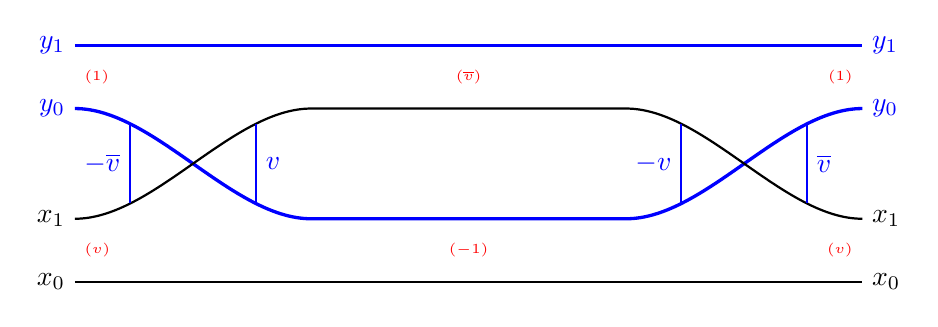
\begin{tikzpicture}%[scale=3]

\draw[very thick,blue] (-5,3)--(5,3);
\draw[very thick,blue] (-5,2.2)..controls (-4,2.2) and (-3,.8)..(-2,.8)--(2,.8)..controls (3,.8) and (4,2.2)..(5,2.2);
\draw[thick] (-5,.8)..controls (-4,.8) and (-3,2.2)..(-2,2.2)--(2,2.2)..controls (3,2.2) and (4,.8)..(5,.8);
\draw[thick] (-5,0)--(5,0);

\draw (-5,0) node[left]{$x_0$};
\draw (-5,.8) node[left]{$x_1$};
\draw (5,.8) node[right]{$x_1$};
\draw (5,0) node[right]{$x_0$};

\draw[blue] (-5,2.2) node[left]{$y_0$};
\draw[blue] (5,2.2) node[right]{$y_0$};
\draw[blue] (-5,3) node[left]{$y_1$};
\draw[blue] (5,3) node[right]{$y_1$};

\draw[thick, blue] (2.7,1)--(2.7,2);
\draw[thick, blue] (-2.7,1)--(-2.7,2);
\draw[blue] (2.7,1.5) node[left]{$-v$};
\draw[blue] (-2.7,1.5) node[right]{$v$};
\draw[thick, blue] (4.3,1)--(4.3,2);
\draw[thick, blue] (-4.3,1)--(-4.3,2);
\draw[blue] (-4.3,1.5) node[left]{$-\overline v$};
\draw[blue] (4.3,1.5) node[right]{$\overline v$};

\draw[red] (0,.4) node{\tiny$(-1)$};
\draw[red] (0,2.6) node{\tiny$(\overline v)$};
\draw[red] (-5,.4) node[right]{\tiny$(v)$};
\draw[red] (-5,2.6) node[right]{\tiny$(1)$};
\draw[red] (5,.4) node[left]{\tiny$(v)$};
\draw[red] (5,2.6) node[left]{\tiny$(1)$};
%\coordinate (A) at (0,0);
%\draw[thick,color=blue] (A) ellipse [x radius=2.8cm,y radius=2.1cm];
\end{tikzpicture}
\caption{Steps  0 and 1 : In the open region between cusps and switch crossing, we introduce two handle slides $x_{12}^{-\overline v}$ and $x_{21}^v$ to put the new sheet $y_0$ in cancelling position with $x_0$. Handle-slides are blue vertical lines and incidence numbers are in red.}
\label{Fig: Step 1-fix open region}
\end{center}
\end{figure}
%
}

{
%
\begin{figure}[htbp]
\begin{center}
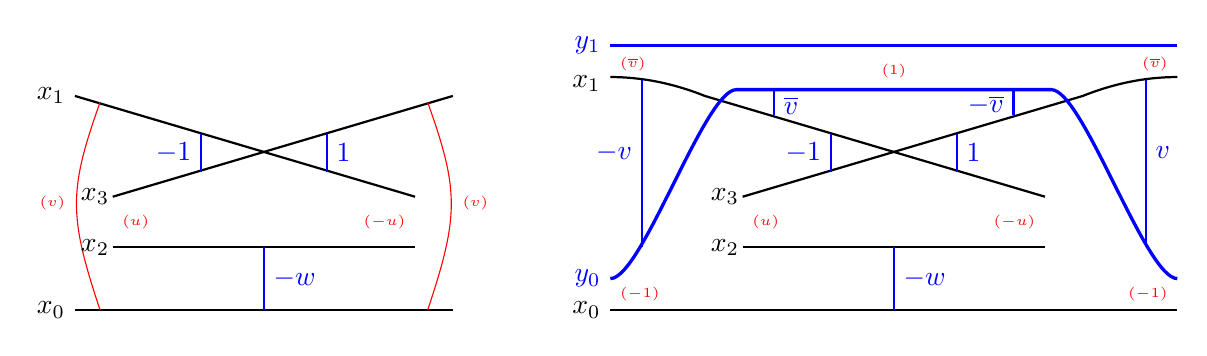
\begin{tikzpicture}[scale=.8]
%\draw[help lines=1,thick] (-5,-5) grid (5,4);

{
\begin{scope}
\draw[thick] (-3,0)--(3,0);
\draw[thick] (-2.4,1)--(2.4,1);
\draw[thick] (-2.4,1.8)--(3,3.4);
\draw[thick] (-3,3.4)--(2.4,1.8);
\draw[thick, blue] (-1,2.2)--(-1,2.8);
\draw[thick, blue] (1,2.2)--(1,2.8);
\draw[thick, blue] (0,0)--(0,1);
\draw[blue] (-1,2.5) node[left]{$-1$};
\draw[blue] (1,2.5) node[right]{$1$};
\draw[blue] (0,.5) node[right]{$-w$};
\draw[red] (-2.4,1.4) node[right]{\tiny$(u)$};
\draw[red] (2.4,1.4) node[left]{\tiny$(-u)$};
\draw[red] (-3,1.7) node[left]{\tiny$(v)$};
\draw[red] (3,1.7) node[right]{\tiny$(v)$};
\draw[red] (-2.6,0)..controls (-3.1,1.5) and (-3.1,1.9)..(-2.6,3.3);
\draw[red] (2.6,0)..controls (3.1,1.5) and (3.1,1.9)..(2.6,3.3);
\draw (-3,0) node[left]{$x_0$};
\draw (-3,3.4) node[left]{$x_1$};
\draw (-2.3,1) node[left]{$x_2$};
\draw (-2.3,1.8) node[left]{$x_3$};

\end{scope}
}

{
\begin{scope}[xshift=10cm]
\draw (-2.3,1.8) node[left]{$x_3$};

\draw (-2.3,1) node[left]{$x_2$};
\draw (-4.5,0) node[left]{$x_0$};
\draw (-4.5,3.6) node[left]{$x_1$};
\draw[blue] (-4.5,0.5) node[left]{$y_0$};
\draw[blue] (-4.5,4.2) node[left]{$y_1$};

\draw[thick] (-4.5,0)--(4.5,0);
\draw[thick] (-2.4,1)--(2.4,1);
\draw[thick] (-2.4,1.8)--(3,3.4)..controls (3.5,3.6) and (4,3.7)..(4.5,3.7);
\draw[thick] (2.4,1.8)--(-3,3.4)..controls (-3.5,3.6) and (-4,3.7)..(-4.5,3.7);
%\draw[thick] (-3,3.4)--(2.4,1.8);
\draw[thick, blue] (-1,2.2)--(-1,2.8);
\draw[thick, blue] (1,2.2)--(1,2.8);
\draw[thick, blue] (0,0)--(0,1);
\draw[blue] (-1,2.5) node[left]{$-1$};
\draw[blue] (1,2.5) node[right]{$1$};
\draw[blue] (0,.5) node[right]{$-w$};
\draw[red] (-2.4,1.4) node[right]{\tiny$(u)$};
\draw[red] (2.4,1.4) node[left]{\tiny$(-u)$};
%
\draw[red] (0,3.8) node{\tiny$(1)$};
\draw[red] (-4.5,3.9) node[right]{\tiny$(\overline v)$};
\draw[red] (4.5,3.9) node[left]{\tiny$(\overline v)$};
\draw[red] (-4.5,.25) node[right]{\tiny$(-1)$};
\draw[red] (4.5,.25) node[left]{\tiny$(-1)$};
%\draw[red] (3,1.7) node[right]{\tiny$(v)$};
\draw[thick,blue] (-4,1)--(-4,3.65);
\draw[thick,blue] (4,1)--(4,3.65);
\draw[blue] (-4,2.5) node[left]{$-v$};
\draw[blue] (4,2.5) node[right]{$v$};
\draw[thick,blue] (-1.9,3.1)--(-1.9,3.5);
\draw[thick,blue] (1.9,3.1)--(1.9,3.5);
\draw[blue] (-1.9,3.25)node[right]{$\overline v$};
\draw[blue] (1.9,3.25)node[left]{$-\overline v$};
%\draw[red] (-2.6,0)..controls (-3.1,1.5) and (-3.1,1.9)..(-2.6,3.3);
%\draw[red] (2.6,0)..controls (3.1,1.5) and (3.1,1.9)..(2.6,3.3);
\draw[very thick,blue] (-4.5,4.2)--(4.5,4.2);
%\draw[very thick,blue] (-4.4,3.3)--(4.4,3.3);
\draw[very thick,blue] (-4.5,.5)..controls (-4,.5) and (-3,3.5)..(-2.5,3.5)--(2.5,3.5)..controls (3,3.5) and (4,.5)..(4.5,.5);%(4.4,.5);
\end{scope}
}


%\draw[thick,color=blue] (A) ellipse [x radius=2.8cm,y radius=2.1cm];
\end{tikzpicture}
\caption{ Steps 0 and 1: On the left we have Step 0 as it appears near a Case (3) switch crossing with sheets $x_0,x_1$ paired as well as  $x_2,x_3$ paired. The $(v), (\pm u)$ indicate incidence matrix entries, while the vertical lines labeled $\pm 1, -w$ are the handle-slides in Figure \ref{fig: exchanges points give 6HS, dual}. On the right, we have applied Step 1, pushing $y_0$ down to $x_0$ away from its cusps and switches.  %Kiyoshi wrote:\color{blue}Step 2a: Case (3) ruling, shown on the left, has two sheets of critical points of index $i-1$. These are $x_0$ and $x_2$. We replace them with index $i+1$ critical points $y_1$ and $y_3$ in two steps. In Step 2 we replace $x_0$ with $y_1$. In Step 0, we introduce two sheets of canceling critical points $y_0,y_1$. In Step 1, we push the $y_0$ sheet down to just above $x_0$ so that $y_0,x_0$ are in cancelling position in the ``open'' region between switch crossings. This gives the figure on the right. Here $w=v\overline u$.
}
\label{Fig: Step 2a- (3) to (1)}
\end{center}
\end{figure}
%
}

{
%
\begin{figure}[htbp]
\begin{center}
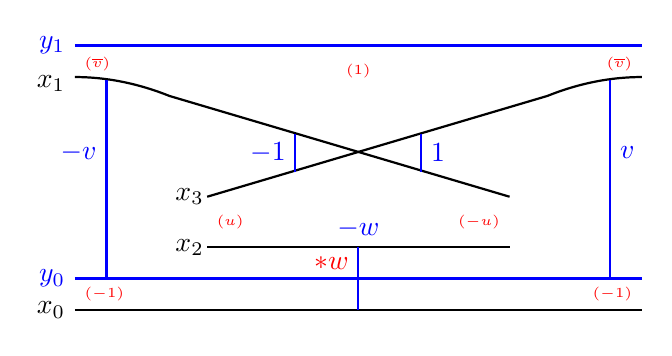
\begin{tikzpicture}[scale=.8]
%\draw[help lines=1,thick] (-5,-5) grid (5,4);

{
\begin{scope}%[xshift=10cm]
\draw (-2.3,1.8) node[left]{$x_3$};

\draw (-2.3,1) node[left]{$x_2$};
\draw (-4.5,0) node[left]{$x_0$};
\draw (-4.5,3.6) node[left]{$x_1$};
\draw[blue] (-4.5,0.5) node[left]{$y_0$};
\draw[blue] (-4.5,4.2) node[left]{$y_1$};

\draw[thick] (-4.5,0)--(4.5,0);
\draw[thick] (-2.4,1)--(2.4,1);
\draw[thick] (-2.4,1.8)--(3,3.4)..controls (3.5,3.6) and (4,3.7)..(4.5,3.7);
\draw[thick] (2.4,1.8)--(-3,3.4)..controls (-3.5,3.6) and (-4,3.7)..(-4.5,3.7);
%\draw[thick] (-3,3.4)--(2.4,1.8);
\draw[thick, blue] (-1,2.2)--(-1,2.8);
\draw[thick, blue] (1,2.2)--(1,2.8);
\draw[thick, blue] (0,0)--(0,1);
\draw[blue] (-1,2.5) node[left]{$-1$};
\draw[blue] (1,2.5) node[right]{$1$};
\draw[blue] (0,1.3) node{$-w$};
\draw[red] (0,.75) node[left]{$\ast w$};
\draw[red] (-2.4,1.4) node[right]{\tiny$(u)$};
\draw[red] (2.4,1.4) node[left]{\tiny$(-u)$};
%
\draw[red] (0,3.8) node{\tiny$(1)$};
\draw[red] (-4.5,3.9) node[right]{\tiny$(\overline v)$};
\draw[red] (4.5,3.9) node[left]{\tiny$(\overline v)$};
\draw[red] (-4.5,.25) node[right]{\tiny$(-1)$};
\draw[red] (4.5,.25) node[left]{\tiny$(-1)$};
%\draw[red] (3,1.7) node[right]{\tiny$(v)$};
\draw[thick,blue] (-4,.5)--(-4,3.65);
\draw[thick,blue] (4,.5)--(4,3.65);
\draw[blue] (-4,2.5) node[left]{$-v$};
\draw[blue] (4,2.5) node[right]{$v$};
%%\draw[thick,blue] (-1.9,3.1)--(-1.9,3.5);
%%\draw[thick,blue] (1.9,3.1)--(1.9,3.5);
%%\draw[blue] (-1.9,3.25)node[right]{$\overline v$};
%%\draw[blue] (1.9,3.25)node[left]{$-\overline v$};
%\draw[red] (-2.6,0)..controls (-3.1,1.5) and (-3.1,1.9)..(-2.6,3.3);
%\draw[red] (2.6,0)..controls (3.1,1.5) and (3.1,1.9)..(2.6,3.3);
\draw[very thick,blue] (-4.5,4.2)--(4.5,4.2);
%\draw[very thick,blue] (-4.4,3.3)--(4.4,3.3);
\draw[very thick,blue] (-4.5,.5)--(4.5,.5);%(4.4,.5);
\end{scope}
}


%\draw[thick,color=blue] (A) ellipse [x radius=2.8cm,y radius=2.1cm];
\end{tikzpicture}
\caption{Step 2: The handle slides $\overline v$ and $-\overline v$ will cancel. Then the $y_0$ sheet can be pushed down as shown on the left. To cancel the unwanted handle slides we introduce an exchange {$\ast w$ (in red)}. This immediately cancel the $-w$ handle slide and creates two new handle slides $v$ and $-v$ which cancel the $-v$ and $v$ handle slides. We are left with a Case (1) ruling with some signs changed plus cancelling sheets $y_0,x_0$ which we ignore.}
\label{Fig: Step 2b- (3) to (1)}
\end{center}
\end{figure}
%
}

{
%
\begin{figure}[htbp]
\begin{center}
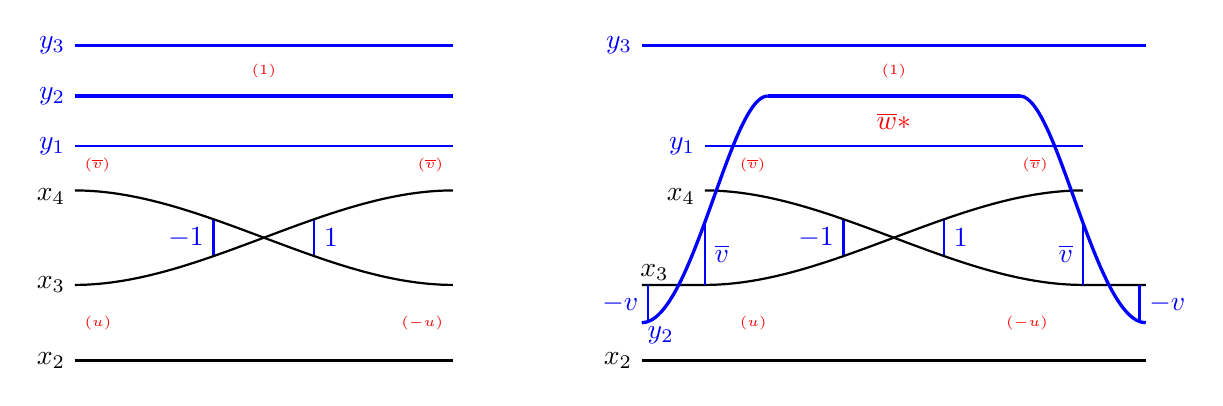
\begin{tikzpicture}[scale=.8]
%\draw[help lines=1,thick] (-5,-5) grid (5,4);

{
\begin{scope}%[xshift=10cm]
\draw[thick,blue] (-.8,1.65)--(-.8,2.25);
\draw[thick,blue] (.8,1.65)--(.8,2.25);
\draw[blue] (-.8,1.95) node[left]{$-1$};
\draw[blue] (.8,1.95) node[right]{$1$};
\draw[thick] (-3,0)--(3,0);
\draw[thick] (-3,1.2)..controls (-1,1.2) and (1,2.7)..(3,2.7);
\draw[thick] (3,1.2)..controls (1,1.2) and (-1,2.7)..(-3,2.7);
\draw[thick,blue] (-3,3.4)--(3,3.4);
\draw[very thick, blue] (-3,4.2)--(3,4.2);
\draw[very thick, blue] (-3,5)--(3,5);
\draw[blue] (-3,4.2)node[left]{$y_2$};
\draw[blue] (-3,5)node[left]{$y_3$};
\draw (-3,0) node[left]{$x_2$};
\draw (-3,1.2) node[left]{$x_3$};
\draw (-3,2.6) node[left]{$x_4$};
\draw[blue] (-3,3.4) node[left]{$y_1$};
\draw[red] (0,4.6) node{\tiny$(1)$};
\draw[red] (-3,.6) node[right]{\tiny$(u)$};
\draw[red] (3,.6) node[left]{\tiny$(-u)$};
\draw[red] (-3,3.1) node[right]{\tiny$(\overline v)$};
\draw[red] (3,3.1) node[left]{\tiny$(\overline v)$};
\end{scope}
}% left figure


{
\begin{scope}[xshift=10cm]
\draw (-3,2.6) node[left]{$x_4$};
\draw[blue] (-3,3.4) node[left]{$y_1$};

\draw[thick,blue] (-.8,1.65)--(-.8,2.25);
\draw[thick,blue] (.8,1.65)--(.8,2.25);
\draw[blue] (-.8,1.95) node[left]{$-1$};
\draw[blue] (.8,1.95) node[right]{$1$};

\draw[thick] (-4,0)--(4,0);
\draw[thick] (-4,1.2)--(-3,1.2)..controls (-1,1.2) and (1,2.7)..(3,2.7);
\draw[thick] (4,1.2)--(3,1.2)..controls (1,1.2) and (-1,2.7)..(-3,2.7);
\draw[thick,blue] (-3,3.4)--(3,3.4);
\draw[very thick, blue] (-2,4.2)--(2,4.2);
\draw[very thick, blue] (-4,5)--(4,5);
\draw[very thick,blue] (-4,.6)..controls (-3.2,.6) and (-2.6,4.2)..(-2,4.2);
\draw[very thick,blue] (4,.6)..controls (3.2,.6) and (2.6,4.2)..(2,4.2);
\draw[blue] (-4,5)node[left]{$y_3$};
\draw (-4,0) node[left]{$x_2$};
\draw[blue] (-3.7,.4)node{$y_2$};
\draw (-3.8,1.4) node{$x_3$};
\draw[thick,blue] (-3.9,.6)--(-3.9,1.2);
\draw[thick,blue] (-3,2.2)--(-3,1.2);
\draw[blue] (-3,1.7) node[right]{$\overline v$};
\draw[blue] (-3.9,.9)node[left]{$-v$};
\draw[thick,blue] (3.9,.6)--(3.9,1.2);
\draw[thick,blue] (3,2.2)--(3,1.2);
\draw[blue] (3,1.7) node[left]{$\overline v$};
\draw[blue] (3.9,.9)node[right]{$-v$};

\draw[red] (0,3.8) node{$\overline w\ast$};

\draw[red] (0,4.6) node{\tiny$(1)$};
\draw[red] (-2.6,.6) node[right]{\tiny$(u)$};
\draw[red] (2.6,.6) node[left]{\tiny$(-u)$};
\draw[red] (-2.6,3.1) node[right]{\tiny$(\overline v)$};
\draw[red] (2.6,3.1) node[left]{\tiny$(\overline v)$};
\end{scope}
}

%\draw[thick,color=blue] (A) ellipse [x radius=2.8cm,y radius=2.1cm];
\end{tikzpicture}
\caption{Step 3a (continuing with notation from Step 2): We have $x_2$ paired with $x_3$ on the left. Step 0 (left): We introduce a pair of cancelling sheets $y_2$ and $y_3$. Step 1 (right):  We push down $y_2$ to be in canceling position with $x_2$ in the ``open region''. Next we go through an exchange $\overline w\ast$ between $y_1$ and $y_2$ where $w=vu$.}
\label{Fig: Step 3a- (1) to (2)}
\end{center}
\end{figure}
%
}

{
%
\begin{figure}[htbp]
\begin{center}
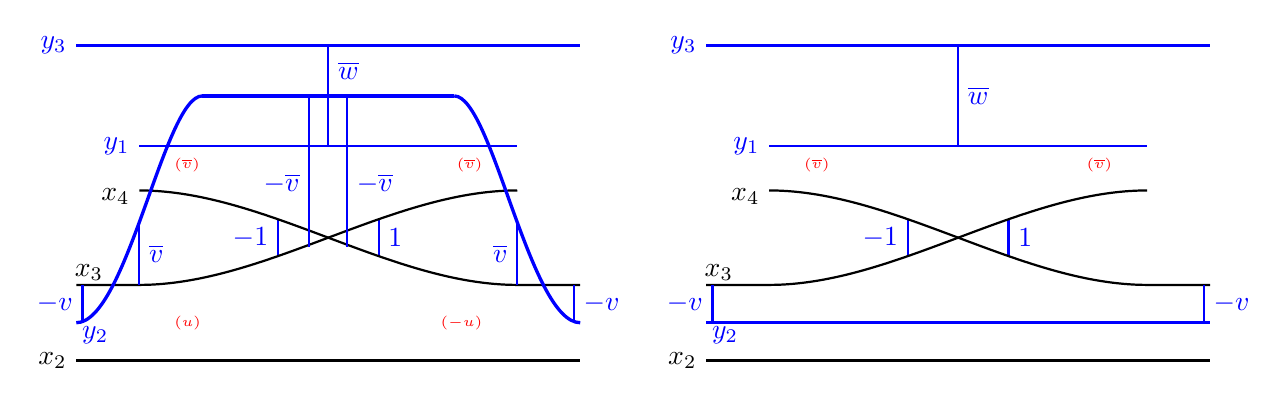
\begin{tikzpicture}[scale=.8]
%\draw[help lines=1,thick] (-5,-5) grid (5,4);

{
\begin{scope}%[xshift=10cm]
\draw (-3,2.6) node[left]{$x_4$};
\draw[blue] (-3,3.4) node[left]{$y_1$};

\draw[thick,blue] (-.8,1.65)--(-.8,2.25);
\draw[thick,blue] (.8,1.65)--(.8,2.25);
\draw[blue] (-.8,1.95) node[left]{$-1$};
\draw[blue] (.8,1.95) node[right]{$1$};

\draw[thick] (-4,0)--(4,0);
\draw[thick] (-4,1.2)--(-3,1.2)..controls (-1,1.2) and (1,2.7)..(3,2.7);
\draw[thick] (4,1.2)--(3,1.2)..controls (1,1.2) and (-1,2.7)..(-3,2.7);
\draw[thick,blue] (-3,3.4)--(3,3.4);
\draw[very thick, blue] (-2,4.2)--(2,4.2);
\draw[very thick, blue] (-4,5)--(4,5);
\draw[very thick,blue] (-4,.6)..controls (-3.2,.6) and (-2.6,4.2)..(-2,4.2);
\draw[very thick,blue] (4,.6)..controls (3.2,.6) and (2.6,4.2)..(2,4.2);
\draw[blue] (-4,5)node[left]{$y_3$};
\draw (-4,0) node[left]{$x_2$};
\draw[blue] (-3.7,.4)node{$y_2$};
\draw (-3.8,1.4) node{$x_3$};
\draw[thick,blue] (-3.9,.6)--(-3.9,1.2);
\draw[thick,blue] (-3,2.2)--(-3,1.2);
\draw[blue] (-3,1.7) node[right]{$\overline v$};
\draw[blue] (-3.9,.9)node[left]{$-v$};
\draw[thick,blue] (3.9,.6)--(3.9,1.2);
\draw[thick,blue] (3,2.2)--(3,1.2);
\draw[blue] (3,1.7) node[left]{$\overline v$};
\draw[blue] (3.9,.9)node[right]{$-v$};

\draw[thick, blue] (0,5)--(0,3.4);
\draw[blue] (0,4.6) node[right]{$\overline w$};
\draw[thick,blue] (.3,4.2)--(.3,1.8);
\draw[thick,blue] (-.3,4.2)--(-.3,1.8);
\draw[blue] (0.3,2.8) node[right]{$-\overline v$};
\draw[blue] (-0.3,2.8) node[left]{$-\overline v$};

%\draw[red] (0,4.6) node{\tiny$(1)$};
\draw[red] (-2.6,.6) node[right]{\tiny$(u)$};
\draw[red] (2.6,.6) node[left]{\tiny$(-u)$};
\draw[red] (-2.6,3.1) node[right]{\tiny$(\overline v)$};
\draw[red] (2.6,3.1) node[left]{\tiny$(\overline v)$};
\end{scope}
}
{
\begin{scope}[xshift=10cm]
\draw (-3,2.6) node[left]{$x_4$};
\draw[blue] (-3,3.4) node[left]{$y_1$};

\draw[thick,blue] (-.8,1.65)--(-.8,2.25);
\draw[thick,blue] (.8,1.65)--(.8,2.25);
\draw[blue] (-.8,1.95) node[left]{$-1$};
\draw[blue] (.8,1.95) node[right]{$1$};

\draw[thick] (-4,0)--(4,0);
\draw[thick] (-4,1.2)--(-3,1.2)..controls (-1,1.2) and (1,2.7)..(3,2.7);
\draw[thick] (4,1.2)--(3,1.2)..controls (1,1.2) and (-1,2.7)..(-3,2.7);
\draw[thick,blue] (-3,3.4)--(3,3.4);
%\draw[very thick, blue] (-2,4.2)--(2,4.2);
\draw[very thick, blue] (-4,5)--(4,5);
\draw[very thick, blue] (-4,.6)--(4,.6);
%\draw[very thick,blue] (-4,.6)..controls (-3.2,.6) and (-2.6,4.2)..(-2,4.2);
%\draw[very thick,blue] (4,.6)..controls (3.2,.6) and (2.6,4.2)..(2,4.2);
\draw[blue] (-4,5)node[left]{$y_3$};
\draw (-4,0) node[left]{$x_2$};
\draw[blue] (-3.7,.4)node{$y_2$};
\draw (-3.8,1.4) node{$x_3$};
\draw[thick,blue] (-3.9,.6)--(-3.9,1.2);
%\draw[thick,blue] (-3,2.2)--(-3,1.2);
%\draw[blue] (-3,1.7) node[right]{$\overline v$};
\draw[blue] (-3.9,.9)node[left]{$-v$};
\draw[thick,blue] (3.9,.6)--(3.9,1.2);
%\draw[thick,blue] (3,2.2)--(3,1.2);
%\draw[blue] (3,1.7) node[left]{$\overline v$};
\draw[blue] (3.9,.9)node[right]{$-v$};

\draw[thick, blue] (0,5)--(0,3.4);
\draw[blue] (0,4.2) node[right]{$\overline w$};

%\draw[red] (0,4.6) node{\tiny$(1)$};
%\draw[red] (-2.6,.6) node[right]{\tiny$(u)$};
%\draw[red] (2.6,.6) node[left]{\tiny$(-u)$};
\draw[red] (-2.6,3.1) node[right]{\tiny$(\overline v)$};
\draw[red] (2.6,3.1) node[left]{\tiny$(\overline v)$};
\end{scope}
}

%\draw[thick,color=blue] (A) ellipse [x radius=2.8cm,y radius=2.1cm];
\end{tikzpicture}
\caption{Step 3b: The exchange point in the deformation in Step 3a produces three handle slides as shown on the left. The two $-\overline v$ hand slides cancel the two $\overline v$ handle slides. Then we can push down the $y_2$ sheet down to $x_2$ as shown on the right. Next, the two $-v$ handle slides come to the center and cancel giving us Case (2) with $y_2,x_2$ cancelling sheets at the bottom.}
\label{Fig: Step 3b- (1) to (2)}
\end{center}
\end{figure}
%
}

{
%
\begin{figure}[htbp] % step 4a
\begin{center}
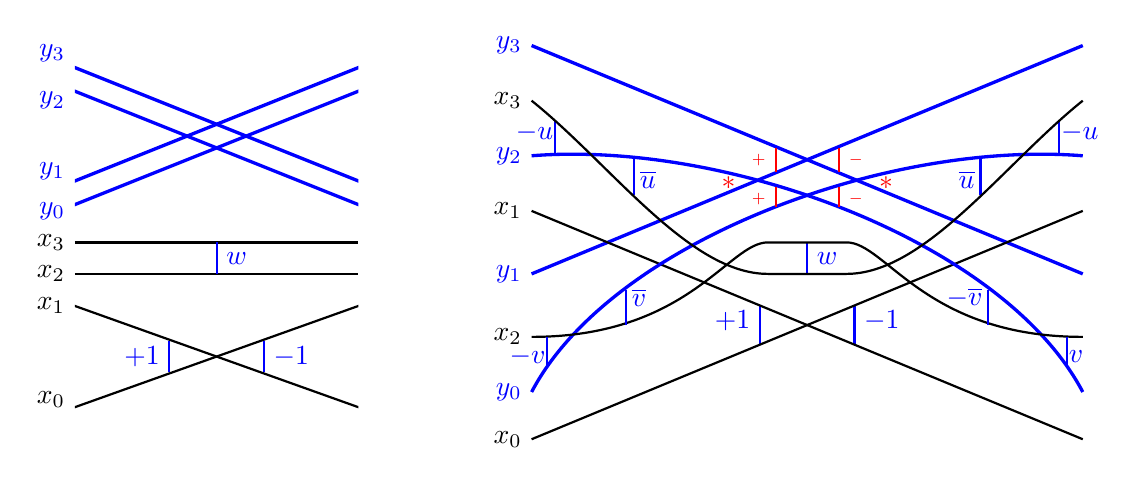
\begin{tikzpicture}%[scale=3]
%\draw[help lines=1,thick] (-5,-5) grid (5,4);
%\foreach \x in {-8,-6,...,8}\draw (\x,0) node{\x};
%\foreach \x/\y in {(0,1)/3,(0,0)/1,(0,-1)/2}
\begin{scope}[xshift=-7.5cm]
\draw (-1.8,0) node[left]{$x_3$};
\draw (-1.8,-.4) node[left]{$x_2$};
\draw (-1.8,-.8) node[left]{$x_1$};
\draw (-1.8,-2) node[left]{$x_0$};
\draw[blue] (-1.8,.4) node[left]{$y_0$};
\draw[blue] (-1.8,.9) node[left]{$y_1$};
\draw[blue] (-1.8,1.8) node[left]{$y_2$};
\draw[blue] (-1.8,2.4) node[left]{$y_3$};
%
\clip (-1.8,-2.3) rectangle (1.8,2.3);
\draw[very thick,blue] (-3.5,-.2)--(3.5,2.6);
\draw[very thick,blue] (-3.5,2.6)--(3.5,-.2);
\draw[very thick,blue] (-3.5,0.1)--(3.5,2.9);
\draw[very thick,blue] (-3.5,2.9)--(3.5,0.1);
\draw[thick] (-3.5,-.2)--(3.5,-2.7);
\draw[thick] (-3.5,-2.7)--(3.5,-.2);
\draw[thick, blue] (-.6,-1.65)--(-.6,-1.25);
\draw[thick, blue] (.6,-1.65)--(.6,-1.25);
\draw[blue] (-.6,-1.45) node[left]{$+1$};
\draw[blue] (.6,-1.45) node[right]{$-1$};
\draw[thick](-1.8,0)--(1.8,0);
\draw[thick](-1.8,-.4)--(1.8,-.4);
\draw[thick, blue] (0,0)--(0,-.4);
\draw[blue] (0,-.2) node[right]{$w$};
\end{scope}



\draw[thick, blue] (-.6,-.8)--(-.6,-1.3);
\draw[thick, blue] (.6,-.8)--(.6,-1.3);
\draw[blue] (-.6,-1.0) node[left]{$+1$};
\draw[blue] (.6,-1.0) node[right]{$-1$};

\draw[thick, blue] (0,0)--(0,-.4);
\draw[blue] (0,-.2) node[right]{$w$};

\draw[very thick,blue] (-3.5,-.4)--(3.5,2.5);
\draw[blue] (-3.5,-.4) node[left]{$y_1$};
\draw[very thick,blue] (-3.5,2.5)--(3.5,-.4);
\draw[blue] (-3.5,2.5) node[left]{$y_3$};
\draw[thick] (-3.5,.4)--(3.5,-2.5);
\draw (-3.5,.4) node[left]{$x_1$};
\draw (-3.5,-2.5) node[left]{$x_0$};
\draw[thick] (-3.5,-2.5)--(3.5,.4);
%\coordinate (A) at (0,0);
\draw[very thick,blue] (-3.5,-1.9)..controls (-2.5,-0) and (1,1.3)..(3.5,1.1);
\draw[very thick,blue] (3.5,-1.9)..controls (2.5,-0) and (-1,1.3)..(-3.5,1.1);
\draw[blue] (-3.5,-1.9) node[left]{$y_0$};
\draw[blue] (-3.5,1.1) node[left]{$y_2$};

\draw[thick, blue] (-3.2,1.1)--(-3.2,1.55);
\draw[blue] (-3.1,1.4) node[left]{$-u$};
\draw[thick, blue] (3.2,1.1)--(3.2,1.55);
\draw[blue] (3.1,1.4) node[right]{$-u$};
\draw[thick, blue] (-2.2,1.1)--(-2.2,.6);
\draw[blue] (-2.25,.8)node[right]{$\overline u$};
\draw[thick, blue] (2.2,1.1)--(2.2,.6);
\draw[blue] (2.25,.8)node[left]{$\overline u$};

\draw[red] (1,.75) node{$\ast$};
\draw[red] (-1,.75) node{$\ast$};

\draw[thick, red] (.4,.9)--(.4,1.2);
\draw[thick, red] (-.4,.9)--(-.4,1.2);
\draw[red] (-.4,1.05) node[left]{\tiny$+$};
\draw[red] (-.4,.55) node[left]{\tiny$+$};
\draw[thick, red] (.4,0.45)--(.4,.7);
\draw[thick, red] (-.4,0.45)--(-.4,.7);
\draw[red] (.4,1.05) node[right]{\tiny$-$};
\draw[red] (.4,.55) node[right]{\tiny$-$};

\draw[thick] (-3.5,-1.2)..controls (-1.5,-1.2) and (-1,0)..(-.5,0)--(.5,0)..controls(1,0)and(1.5,-1.2)..(3.5,-1.2);
\draw (-3.5,-1.2) node[left]{$x_2$};

\draw[thick, blue] (-3.3,-1.2)--(-3.3,-1.6);
\draw[blue] (-3.2,-1.45) node[left]{$-v$};
\draw[thick, blue] (-2.3,-1.05)--(-2.3,-.6);
\draw[blue] (-2.35,-.7) node[right]{$\overline v$};

\draw[thick, blue] (3.3,-1.2)--(3.3,-1.6);
\draw[blue] (3.2,-1.45) node[right]{$v$};
\draw[thick, blue] (2.3,-1.05)--(2.3,-.6);
\draw[blue] (2.35,-.7) node[left]{$-\overline v$};


\draw[thick] (-3.5,1.8) ..controls (-2.5,1) and (-1.5,-.4)..(-.5,-.4)--(0,-.4);
\draw (-3.5,1.8) node[left]{$x_3$};
\draw[thick] (3.5,1.8) ..controls (2.5,1) and (1.5,-.4)..(.5,-.4)--(0,-.4);
%\draw[thick,color=blue] (A) ellipse [x radius=2.8cm,y radius=2.1cm];
\end{tikzpicture}
\caption{Step 4a: In the left subfigure, we have the Case (2) ruling with paired sheets $x_0,x_3$ and $x_1,x_2$ on the left side and $x_1,x_3$ and $x_0,x_2$ on the right side. We added two pairs of canceling sheets $y_1/y_0$ and $y_3/y_2$. After Step 1 we have the figure on the right. Next (in red), we introduce two exchange points producing four new handle slides at the top.} %We need to put $y_0/x_0$ and $y_2/x_2$ into canceling position.}
\label{Fig: Step 4a}
\end{center}
\end{figure}
%
}






{
%
\begin{figure}[htbp]% step 4b
\begin{center}
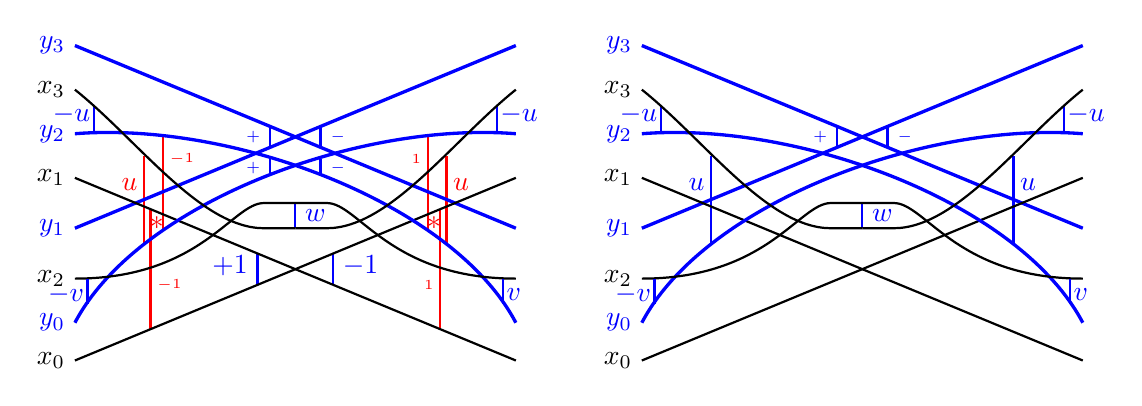
\begin{tikzpicture}[scale=.8]
{
\begin{scope}
\draw[red] (2.2,-.32) node{$\ast$};
\draw[red] (-2.2,-.32) node{$\ast$};

\draw[thick,red] (-2.4,-.65)--(-2.4,.75);
\draw[red] (-2.35,.3) node[left]{$u$};
\draw[thick,red] (2.4,-.65)--(2.4,.75);
\draw[red] (2.35,.3) node[right]{$u$};

\draw[thick,red] (-2.3,-2)--(-2.3,-.1);
\draw[red] (-2.35,-1.3) node[right]{\tiny$-1$};
\draw[thick,red] (-2.1,-.43)--(-2.1,1.09);
\draw[red] (-2.15, .7) node[right]{\tiny$-1$};

\draw[thick,red] (2.3,-2)--(2.3,-.1);
\draw[red] (2.35,-1.3) node[left]{\tiny$1$};
\draw[thick,red] (2.1,-.43)--(2.1,1.09);
\draw[red] (2.15, .7) node[left]{\tiny$1$};

\draw[thick, blue] (-.6,-.8)--(-.6,-1.3);
\draw[thick, blue] (.6,-.8)--(.6,-1.3);
\draw[blue] (-.6,-1.0) node[left]{$+1$};
\draw[blue] (.6,-1.0) node[right]{$-1$};

\draw[thick, blue] (0,0)--(0,-.4);
\draw[blue] (0,-.2) node[right]{$w$};

\draw[very thick,blue] (-3.5,-.4)--(3.5,2.5);
\draw[blue] (-3.5,-.4) node[left]{$y_1$};
\draw[very thick,blue] (-3.5,2.5)--(3.5,-.4);
\draw[blue] (-3.5,2.5) node[left]{$y_3$};
\draw[thick] (-3.5,.4)--(3.5,-2.5);
\draw (-3.5,.4) node[left]{$x_1$};
\draw (-3.5,-2.5) node[left]{$x_0$};
\draw[thick] (-3.5,-2.5)--(3.5,.4);
%\coordinate (A) at (0,0);
\draw[very thick,blue] (-3.5,-1.9)..controls (-2.5,-0) and (1,1.3)..(3.5,1.1);
\draw[very thick,blue] (3.5,-1.9)..controls (2.5,-0) and (-1,1.3)..(-3.5,1.1);

\draw[blue] (-3.5,-1.9) node[left]{$y_0$};
\draw[blue] (-3.5,1.1) node[left]{$y_2$};

\draw[thick, blue] (-3.2,1.1)--(-3.2,1.55);
\draw[blue] (-3.1,1.4) node[left]{$-u$};
\draw[thick, blue] (3.2,1.1)--(3.2,1.55);
\draw[blue] (3.1,1.4) node[right]{$-u$};

\draw[thick, blue] (.4,.9)--(.4,1.2);
\draw[thick, blue] (-.4,.9)--(-.4,1.2);
\draw[blue] (-.4,1.05) node[left]{\tiny$+$};
\draw[blue] (-.4,.55) node[left]{\tiny$+$};
\draw[thick, blue] (.4,0.45)--(.4,.7);
\draw[thick, blue] (-.4,0.45)--(-.4,.7);
\draw[blue] (.4,1.05) node[right]{\tiny$-$};
\draw[blue] (.4,.55) node[right]{\tiny$-$};

\draw[thick] (-3.5,-1.2)..controls (-1.5,-1.2) and (-1,0)..(-.5,0)--(.5,0)..controls(1,0)and(1.5,-1.2)..(3.5,-1.2);
\draw (-3.5,-1.2) node[left]{$x_2$};

\draw[thick, blue] (-3.3,-1.2)--(-3.3,-1.6);
\draw[blue] (-3.2,-1.45) node[left]{$-v$};

\draw[thick, blue] (3.3,-1.2)--(3.3,-1.6);
\draw[blue] (3.2,-1.45) node[right]{$v$};

\draw[thick] (-3.5,1.8) ..controls (-2.5,1) and (-1.5,-.4)..(-.5,-.4)--(0,-.4);
\draw (-3.5,1.8) node[left]{$x_3$};
\draw[thick] (3.5,1.8) ..controls (2.5,1) and (1.5,-.4)..(.5,-.4)--(0,-.4);
\end{scope}
}
{
\begin{scope}[xshift=9cm]
%\draw[red] (2.2,-.32) node{$\ast$};
%\draw[red] (-2.2,-.32) node{$\ast$};

\draw[thick,blue] (-2.4,-.65)--(-2.4,.75);
\draw[blue] (-2.35,.3) node[left]{$u$};
\draw[thick,blue] (2.4,-.65)--(2.4,.75);
\draw[blue] (2.35,.3) node[right]{$u$};



\draw[thick, blue] (0,0)--(0,-.4);
\draw[blue] (0,-.2) node[right]{$w$};

\draw[very thick,blue] (-3.5,-.4)--(3.5,2.5);
\draw[blue] (-3.5,-.4) node[left]{$y_1$};
\draw[very thick,blue] (-3.5,2.5)--(3.5,-.4);
\draw[blue] (-3.5,2.5) node[left]{$y_3$};
\draw[thick] (-3.5,.4)--(3.5,-2.5);
\draw (-3.5,.4) node[left]{$x_1$};
\draw (-3.5,-2.5) node[left]{$x_0$};
\draw[thick] (-3.5,-2.5)--(3.5,.4);
%\coordinate (A) at (0,0);
\draw[very thick,blue] (-3.5,-1.9)..controls (-2.5,-0) and (1,1.3)..(3.5,1.1);
\draw[very thick,blue] (3.5,-1.9)..controls (2.5,-0) and (-1,1.3)..(-3.5,1.1);
\draw[blue] (-3.5,-1.9) node[left]{$y_0$};
\draw[blue] (-3.5,1.1) node[left]{$y_2$};

\draw[thick, blue] (-3.2,1.1)--(-3.2,1.55);
\draw[blue] (-3.1,1.4) node[left]{$-u$};
\draw[thick, blue] (3.2,1.1)--(3.2,1.55);
\draw[blue] (3.1,1.4) node[right]{$-u$};

\draw[thick, blue] (.4,.9)--(.4,1.2);
\draw[thick, blue] (-.4,.9)--(-.4,1.2);
\draw[blue] (-.4,1.05) node[left]{\tiny$+$};
%\draw[blue] (-.4,.55) node[left]{\tiny$+$};
%\draw[thick, blue] (.4,0.45)--(.4,.7);
%\draw[thick, blue] (-.4,0.45)--(-.4,.7);
\draw[blue] (.4,1.05) node[right]{\tiny$-$};
%\draw[blue] (.4,.55) node[right]{\tiny$-$};

\draw[thick] (-3.5,-1.2)..controls (-1.5,-1.2) and (-1,0)..(-.5,0)--(.5,0)..controls(1,0)and(1.5,-1.2)..(3.5,-1.2);
\draw (-3.5,-1.2) node[left]{$x_2$};

\draw[thick, blue] (-3.3,-1.2)--(-3.3,-1.6);
\draw[blue] (-3.2,-1.45) node[left]{$-v$};

\draw[thick, blue] (3.3,-1.2)--(3.3,-1.6);
\draw[blue] (3.2,-1.45) node[right]{$v$};

\draw[thick] (-3.5,1.8) ..controls (-2.5,1) and (-1.5,-.4)..(-.5,-.4)--(0,-.4);
\draw (-3.5,1.8) node[left]{$x_3$};
\draw[thick] (3.5,1.8) ..controls (2.5,1) and (1.5,-.4)..(.5,-.4)--(0,-.4);
\end{scope}
}
%\draw[thick,color=blue] (A) ellipse [x radius=2.8cm,y radius=2.1cm];
\end{tikzpicture}
\caption{Step 4b: Continuing from Step 4a, we can now cancel the four handle slides labeled $\overline u,\pm\overline v$. More precisely, the $\overline v$ and $-\overline v$ can be brought to the middle and cancelled. When they pass over th $w$ handle slide they produce two $-\overline u$ which cancel the $\overline u$ handle slide. We have deleted these. Next (in red) we pass through two exchanges, producing 6 more handle slide, 4 of them will cancel the bottom four $\pm1$ handle slides. We get the figure on the right.
} %We need to put $y_0/x_0$ and $y_2/x_2$ into canceling position.}
\label{Fig: Step 4b}
\end{center}
\end{figure}
%
}

{
%
\begin{figure}[htbp] %Step 4c
\begin{center}
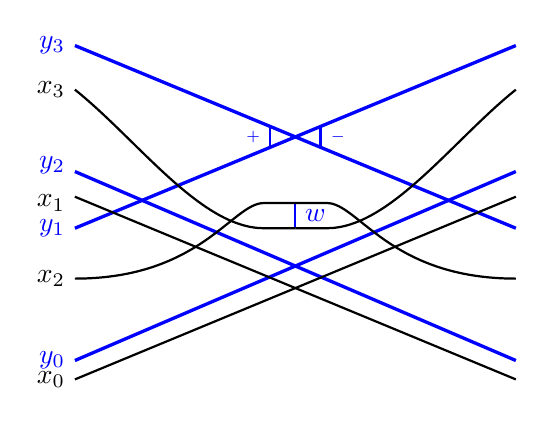
\begin{tikzpicture}[scale=.8]

{
\begin{scope}

\draw[thick, blue] (0,0)--(0,-.4);
\draw[blue] (0,-.2) node[right]{$w$};

\draw[very thick,blue] (-3.5,-.4)--(3.5,2.5);
\draw[blue] (-3.5,-.4) node[left]{$y_1$};
\draw[very thick,blue] (-3.5,2.5)--(3.5,-.4);
\draw[blue] (-3.5,2.5) node[left]{$y_3$};
%\coordinate (A) at (0,0);

\begin{scope}[yshift=-.6cm]
\draw[blue] (-3.5,-1.9) node[left]{$y_0$};
\draw[blue] (-3.5,1.2) node[left]{$y_2$}; %Step 4c
\draw[very thick,blue] (-3.5,-1.9)--(3.5,1.1);
\draw[very thick,blue] (3.5,-1.9)--(-3.5,1.1);
\end{scope}
\begin{scope}[yshift=-.3cm]
\draw (-3.5,-2.5) node[left]{$x_0$};
\draw[thick] (-3.5,-2.5)--(3.5,.4);
\draw[thick] (-3.5,.4)--(3.5,-2.5);
\draw (-3.5,.3) node[left]{$x_1$};
\end{scope}

\draw[thick, blue] (.4,.9)--(.4,1.2);
\draw[thick, blue] (-.4,.9)--(-.4,1.2);
\draw[blue] (-.4,1.05) node[left]{\tiny$+$};
\draw[blue] (.4,1.05) node[right]{\tiny$-$};

\draw[thick] (-3.5,-1.2)..controls (-1.5,-1.2) and (-1,0)..(-.5,0)--(.5,0)..controls(1,0)and(1.5,-1.2)..(3.5,-1.2);
\draw (-3.5,-1.2) node[left]{$x_2$};


\draw[thick] (-3.5,1.8) ..controls (-2.5,1) and (-1.5,-.4)..(-.5,-.4)--(0,-.4);
\draw (-3.5,1.8) node[left]{$x_3$};
\draw[thick] (3.5,1.8) ..controls (2.5,1) and (1.5,-.4)..(.5,-.4)--(0,-.4);
\end{scope}
}
%\draw[thick,color=blue] (A) ellipse [x radius=2.8cm,y radius=2.1cm];
\end{tikzpicture}
\caption{Step 4c: We push down the $y_0$ and $y_2$ sheets until they are right above the $x_0$ and $x_1$ sheets. Then all the $u$ and $v$ handle slides cancel. We obtain ruling Case (3) with two pairs of cancelling sheets below.
} %We need to put $y_0/x_0$ and $y_2/x_2$ into canceling position.}
\label{Fig: Step 4c}
\end{center}
\end{figure}
%
}

{
%
\begin{figure}[htbp]
\begin{center}
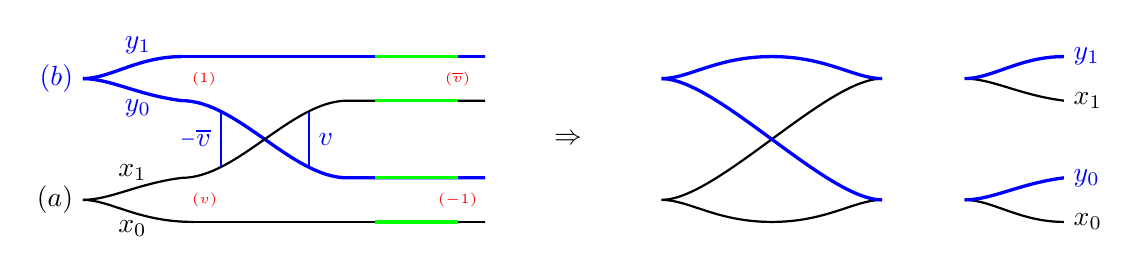
\begin{tikzpicture}[scale=.7]
%\draw[help lines=1,thick] (-5,-5) grid (5,4);
%\foreach \x in {-8,-6,...,8}\draw (\x,0) node{\x};
%\foreach \x/\y in {(0,1)/3,(0,0)/1,(0,-1)/2}
\begin{scope}[xshift=10cm]%right subfigure
\begin{scope}[yshift=4mm,xshift=-.8cm] 
\draw[blue] (1.8,.4) node[right]{$y_0$};
\draw[blue] (1.8,2.6) node[right]{$y_1$};
\draw (1.8,-.4) node[right]{$x_0$};
\draw (1.8,1.8) node[right]{$x_1$};
\draw[thick] (0,0)..controls (.5,0) and (1,-.4)..(1.8,-.4);
\draw[very thick,blue] (0,0)..controls (.5,0) and (1,.3)..(1.8,.4);
\draw[thick] (0,2.2)..controls (.5,2.2) and (1,1.9)..(1.8,1.8);
\draw[very thick,blue] (0,2.2)..controls (.5,2.2) and (1,2.6)..(1.8,2.6);
\begin{scope}[xshift=5mm]
\draw[thick] (-6,0)..controls (-5.5,0) and (-5,-.4)..(-4,-.4);
\draw[thick] (-2,0)..controls (-2.5,0) and (-3,-.4)..(-4,-.4);
\draw[thick] (-6,0)..controls (-5,0) and (-3,2.2)..(-2,2.2);
\draw[very thick,blue] (-6,2.2)..controls (-5,2.2) and (-3,0)..(-2,0);
%
\begin{scope}[yshift=2.2cm]
\draw[very thick,blue] (-6,0)..controls (-5.5,0) and (-5,.4)..(-4,.4);
\draw[very thick,blue] (-2,0)..controls (-2.5,0) and (-3,.4)..(-4,.4);
\end{scope}
\end{scope}
\end{scope}


\end{scope}

\draw(2,1.5)node{$\Rightarrow$};
\begin{scope}[yshift=4mm,xshift=-6.8cm] %left subfigure

\draw (0,0) node[left]{$(a)$};
\draw[blue] (0,2.2) node[left]{$(b)$};
\draw[blue] (1,2) node[below]{$y_0$};
\draw[blue] (1,2.8) node{$y_1$};
\draw[thick] (0,0)..controls (.5,0) and (1,-.4)..(2,-.4);
\draw[thick] (0,0)..controls (.5,0) and (1,.3)..(1.8,.4);
\draw[very thick,blue] (0,2.2)..controls (.5,2.2) and (1,1.9)..(1.8,1.8);
\draw[very thick,blue] (0,2.2)..controls (.5,2.2) and (1,2.6)..(1.8,2.6);
\end{scope}

\begin{scope}
\draw (-5.9,0.2) node[below]{$x_0$};
\draw (-5.9,.9) node{$x_1$};

\clip (-5,-.1)rectangle (0.5,3.1);
\draw[very thick,blue] (-5,3)--(5,3);
\draw[very thick,blue] (-5,2.2)..controls (-4,2.2) and (-3,.8)..(-2,.8)--(2,.8)..controls (3,.8) and (4,2.2)..(5,2.2);
\draw[thick] (-5,.8)..controls (-4,.8) and (-3,2.2)..(-2,2.2)--(2,2.2)..controls (3,2.2) and (4,.8)..(5,.8);
\draw[thick] (-5,0)--(5,0);


\draw[blue] (-5,2.2) node[left]{$y_0$};
%\draw[blue] (5,2.2) node[right]{$y_0$};
\draw[blue] (-5,3) node[left]{$y_1$};
%\draw[blue] (5,3) node[right]{$y_1$};

\draw[thick, blue] (-2.7,1)--(-2.7,2);
\draw[blue] (-2.7,1.5) node[right]{$v$};
\draw[thick, blue] (-4.3,1)--(-4.3,2);
\draw[blue] (-4.3,1.5) node[left]{$-\overline v$};

\draw[red] (0,.4) node{\tiny$(-1)$};
\draw[red] (0,2.6) node{\tiny$(\overline v)$};
\draw[red] (-5,.4) node[right]{\tiny$(v)$};
\draw[red] (-5,2.6) node[right]{\tiny$(1)$};

\draw[very thick,green] (-1.5,0)--(0,0);
\draw[very thick,green] (-1.5,0.8)--(0,0.8);
\draw[very thick,green] (-1.5,2.2)--(0,2.2);
\draw[very thick,green] (-1.5,3)--(0,3);
\end{scope}

%\foreach \y in {-6,-4,...,8}\draw (0,\y) node{\y};
%\coordinate (A) at (0,0);
%\draw[thick,color=blue] (A) ellipse [x radius=2.8cm,y radius=2.1cm];
\end{tikzpicture}
\caption{The cusp $(a)$ on the left produces cusp $(b)$ in Step 0. The new $y_0$ sheet is pushed down on top of the $x_0$ sheet in Step 1. We cancel the green pairs to obtain the figure on the right. This gives the desired result together with a ``figure 8'' which we can ignore since it contributes 0 to the torsion as explained in the text.}
\label{Fig: Step 5}
\end{center}
\end{figure}
%
}

{
%
\begin{figure}[htbp]
\begin{center}
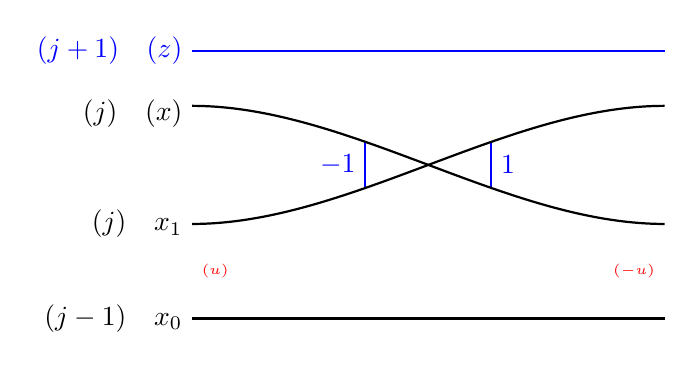
\begin{tikzpicture}%[scale=3]
{
\begin{scope}%[xshift=10cm]
\draw[thick,blue] (-.8,1.65)--(-.8,2.25);
\draw[thick,blue] (.8,1.65)--(.8,2.25);
\draw[blue] (-.8,1.95) node[left]{$-1$};
\draw[blue] (.8,1.95) node[right]{$1$};
\draw[thick] (-3,0)--(3,0);
\draw[thick] (-3,1.2)..controls (-1,1.2) and (1,2.7)..(3,2.7);
\draw[thick] (3,1.2)..controls (1,1.2) and (-1,2.7)..(-3,2.7);
\draw[thick,blue] (-3,3.4)--(3,3.4);
%\draw[very thick, blue] (-3,4.2)--(3,4.2);
%\draw[very thick, blue] (-3,5)--(3,5);
%\draw[blue] (-3,4.2)node[left]{$y_2$};
%\draw[blue] (-3,5)node[left]{$y_3$};
\draw (-3,0) node[left]{$(j-1)\quad x_0$};
\draw (-3,1.2) node[left]{$(j)\quad x_1$};
\draw (-3,2.6) node[left]{$(j)\quad (x)$};
\draw[blue] (-3,3.4) node[left]{$(j+1)\quad (z)$};
%\draw[red] (0,4.6) node{\tiny$(1)$};
\draw[red] (-3,.6) node[right]{\tiny$(u)$};
\draw[red] (3,.6) node[left]{\tiny$(-u)$};
%\draw[red] (-3,3.1) node[right]{\tiny$(\overline v)$};
%\draw[red] (3,3.1) node[left]{\tiny$(\overline v)$};
\end{scope}
}
%\coordinate (A) at (0,0);
%\draw[thick,color=blue] (A) ellipse [x radius=2.8cm,y radius=2.1cm];
\end{tikzpicture}
\caption{When the unpaired sheet $(x)$ switches with a sheet $x_1$ which is paired with a sheet $x_0$ in index $j-1$, we need to trade sheet $x_0$ up to a sheet $y_1$ of index $j+1$. First we bring down the 0-section $(z)$ which we are pairing with the unpaired sheet $(x)$. This produces Case 1 in Figure \ref{fig: Rulings} and we proceed as in Step 3a in Figure \ref{Fig: Step 3a- (1) to (2)}.}
\label{Fig: unpaired sheet}
\end{center}
\end{figure}
%
}


\subsection{A ruling implies a generating family}
\label{sec: RulingGeneratingFamily}
In this subsection $\Lambda$ is a Legendrian, which is not necessarily the lift of a nearby Lagrangian.
We do not assume $\Lambda$ has a generating family, but do assume it has a ruling.
We no longer assume Hypothesis H.

\begin{theorem}
\label{thm: RulingGeneratingFamily}
The Legendrian $\Lambda$ has a generating family.
Up to some global constant in degree, the rank of the generating family's fiber homology in degree $i$ equals the number of unpaired sheets with Maslov potential $i.$
\end{theorem}

\begin{proof}
We repeat the construction-proof in Section \ref{sec: RulingTorsion}.
In Part 1a,  we construct the generating family for the two-copy $\Lambda \cup \Lambda_\epsilon.$
In Part 1b, we use the ruling to build handle-slides near the switches.
In Part 1c, we shift $\Lambda_t$ in the positive $z$-direction.
Note that at this point we have a Legendrian homotopy instead of isotopy:  Reeb chords of $\Lambda$ correspond to intersections of $\Lambda_t$ and $\Lambda$ for some $t.$
However, the accounting of handle-slides done in Parts 1d, 2a, 2b, 2c, 2d implies that there is no Morse-theory obstruction to shifting $\Lambda_t$ up.
In particular, there is no fiberwise negative gradient flowline from a sheet of $\Lambda$ to a sheet of $\Lambda_t$ that shrinks to 0.

But now consider the incidence matrices for the unpaired sheets.
For each sheet (in each fiber) there is a single negative gradient flow from the unpaired sheet of $\Lambda_T$ to the corresponding unparied sheet of $\Lambda.$
When we cut off the generating family as done at the outset of Part 2, 
these unpaired sheets correspond to generators of the fiber homology.

\end{proof}
\end{comment}


\appendix


\section{Moderate singularities}\label{sec: moderate singularities}

\subsection{Functions with moderate singularities}

For $F$ a smooth manifold, a function $f:F \to \bR$ has {\em moderate singularities} if its singularities are modeled on either the Morse normal form $$\sum_{i\leq k}x_i^2-\sum_{i>k}x_i^2$$ or on the cubic (birth/death) form $$x_1^3+\sum_{1<i\leq k}x_i^2-\sum_{i>k}x_i^2.$$ 
Note that at a birth/death point of $f$, the kernel of the hessian $d^2f$ is one dimensional and is trivialized by the direction in which $d^3f$ is positive. We call this the {\em canonical co-orientation}. See Figure \ref{Figure1904}.

{
%
\begin{figure}[htbp]
\begin{center}
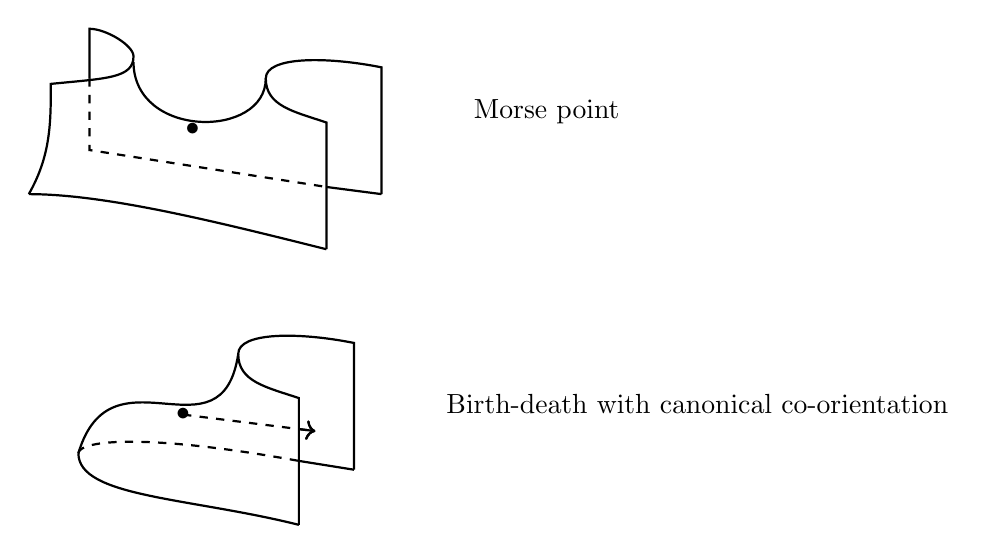
\begin{tikzpicture}[scale=.7]
%\draw[help lines=1,thin] (-2,-2) grid (5,4);
%\foreach \x in {-2,...,5}\draw (\x,0) node{\x};
%\foreach \x/\y in {(0,1)/3,(0,0)/1,(0,-1)/2}
%\foreach \y in {-4,...,4}\draw (0,\y) node{\y};
%
\begin{scope}% birth-death
%\draw[thick,red] (-.4,0)..controls (0,.7) and (0,1.3)..(0,2)..controls (1,2.1) and (1.5,2.1)..(1.5,2.5)..controls (1.5,2.7) and (1,3).. (.7,3)--(.7,2.1); % left
\draw[thick] (1,0.3)..controls (1.6,2.3) and (3.6,.1)..(3.9,2.1); %birth-death 
\draw[thick] (1,0.3)..controls (1,-.5) and (3,-.5)..(5,-1); % bottom front
\draw[thick] (5,-1)--(5,1.3)..controls (4.4,1.5) and ( 3.9,1.6)..(3.9,2.1)..controls (3.9,2.5) and (5,2.5) .. (6,2.3)--(6,0); %right edge
\draw[dashed,thick] (1,0.3)..controls (1,.5) and (2,.7)..(5,0.16);
\draw[thick] (5,0.16)--(6,0);
\draw (2.9,1) node{$\bullet$};
\draw[thick,dashed,->] (2.9,1)--(5.3,.7);
\draw (7.5,1.2) node[right]{Birth-death with canonical co-orientation};
\clip (5,0) rectangle (5.6,1);
\draw[thick,->] (2.9,1)--(5.3,.7);


%\draw[thick]
\end{scope}
%
%
\begin{scope}[yshift=5cm,xshift=.5cm]% saddle
%\draw[help lines=1,thin] (-2,-2) grid (5,4);
%\foreach \x in {-2,...,5}\draw (\x,0) node{\x};
\draw (2.57,1.17) node{$\bullet$};
\draw[thick] (-.4,0)..controls (0,.7) and (0,1.3)..(0,2)..controls (1,2.1) and (1.5,2.1)..(1.5,2.5)..controls (1.5,2.7) and (1,3).. (.7,3)--(.7,2.1); % left edge
\draw[thick] (1.5,2.4)..controls (1.5,1) and (3.9,1)..(3.9,2.1); %saddle 
\draw[thick] (-.4,0)..controls (1,0) and (3,-.5)..(5,-1); % front bottom
\draw[thick] (5,-1)--(5,1.3)..controls (4.4,1.5) and ( 3.9,1.6)..(3.9,2.1)..controls (3.9,2.5) and (5,2.5) .. (6,2.3)--(6,0); %right edge
\draw[dashed,thick] (.7,2.1)--(.7,.8)--(5,0.13);
\draw[thick] (5,0.13)--(6,0);
\draw (7.5,1.5) node[right]{Morse point};
%\draw[thick]
\end{scope}
%
%\coordinate (A) at (0,0);
%\draw[thick,color=blue] (A) ellipse [x radius=2.8cm,y radius=2.1cm];
\end{tikzpicture}
\caption{Morse and birth-death points.} %fig 1904
\label{Figure1904}
\end{center}
\end{figure}
%
}

For $F \to W \to M$ a fiber bundle, a function $f:W \to \bR$ has {\em moderate singularities} if each restriction $f|_m:F_m \to \bR$ to the fiber over $m \in M$ has moderate singularities and if moreover the fibered singularities  of $f$ over $M$ 
\[
\begin{tikzcd}
W \arrow[dr]  \arrow[rr, "f"] &    & M \times \bR \arrow[dl] \\
& M & 
\end{tikzcd}
\]
are modeled on either a constant family of Morse critical points
$$ (t_1,\ldots,t_m,x_1,\ldots,x_N)\mapsto  (t_1,\ldots,t_m, \sum_{i\leq k}x_i^2-\sum_{i>k}x_i^2) $$
or a fibered birth/death of Morse critical points 
$$(t_1,\ldots,t_m, x_1,\ldots,x_N) \mapsto (t_1,\ldots, t_m, x_1^3+3t_1x_1 + \sum_{1<i\leq k}x_i^2 - \sum_{i >k}x_i^2 )$$
with both families fibered over $(t_1,\ldots,t_m)$ with respect to the obvious projection. If $M$ has boundary we will allow one-half of the above fibered models, i.e. restricting the fibration to a half space of the base. 

\subsection{The stable bundle}

Let $F \to W \to M$ be a fiber bundle and let $f:W \to \bR$ be a function with moderate singularities. The fiberwise singular set $\Sigma_f \subset W$ is a smooth submanifold of $W$ of the same dimension as $M$. It has a stratification $\Sigma_f = \bigcup_k \Sigma_{f,k}$ where $\Sigma_{f,k}$ is the closure of the set of fiberwise Morse critical points of index $k$. Let $C_{f,k} \subset \Lambda_f$ consist of the set of fiberwise cubic (birth/death) critical points of $f$ of index $k$ and $k+1$. So the boundary of $\Lambda_{f,k}$ consists of the disjoint union of $C_{f,k-1}$ and $C_{f,k}$. %\footnote{\color{orange}Mike: I don't understand this last sentence.}

On the interior of $\Sigma_{f,k}$ we have a rank $k$ real vector bundle $\gamma_{f,k} \to \Sigma_{f,k}$ consisting of the negative eigenspace of the fiberwise Hessian along the fiberwise critical locus. Each $\gamma_{f,k}$ extends to the boundary $C_{f,k} \coprod C_{f,k-1}$ of $\Sigma_{f,k}$ as sub-bundles of the fiberwise tangent bundle of $W$, but along $C_{f,k}$ the dimensions of $\gamma_{f,k}$ and $\gamma_{f,k+1}$ jump by one. More precisely, we have the relation $\gamma_{f,k}\oplus \nu_k= \gamma_{f,k+1}$ where $\nu_k$ is the kernel of the Hessian, a rank 1 bundle along $C_{f,k}$. So we may form a vector bundle over $\Sigma_f=\bigcup_k \Sigma_{f,k}$ by using the canonical co-orientation to glue the vector bundles $\gamma_{f,k} \oplus \ve^{N-k}$ on $\Sigma_{f,k}$, where $\ve$ denotes the trivial rank 1 bundle, to a rank $N$ vector bundle on $\Sigma_f$. More precisely, the canonical co-orientation gives a trivialization $\nu_k \simeq \ve$ and so we may glue via the vector bundle isomorphism over $C_{f,k}$ given by
$$ \gamma_{f,k} \oplus \ve^{N-k} \simeq \gamma_{f,k} \oplus \nu_k \oplus \ve^{N-k-1} \simeq \gamma_{f,k+1} \oplus \ve^{N-k-1} .$$
We denote the stable class of this real vector bundle over $\Sigma_f$ by $\gamma_f$ and will refer to it as the {\em stable bundle} of $f$. 

\subsection{Framed functions}

For $F \to W \to M$ a fiber bundle, a framed function $f:W \to \bR$ is roughly speaking a function with moderate singularities whose stable bundle $\gamma_f$ is trivial and moreover equipped with a trivialization. More precisely, one requires the existence of isomorphisms $$\varphi_k: \gamma_{f,k} \xrightarrow{\simeq} \ve^k$$ which are compatible with the above gluing maps. We will refer to the following result as the {\em framed function theorem}.

\begin{theorem}\label{thm: framed function}
For $F \to W \to M$ a fiber bundle, given a closed subset $A \subset W$ and a framed function $g:Op(A) \to \bR$ there exists a framed function $f:W \to \bR$ which agrees with $g$ on $Op(A)$. 
\end{theorem}

In particular, for any fiber bundle $F \to W \to M$ framed functions $f:W \to \bR$ exist, and if $f_0$ and $f_1$ are two such then there exists a framed function $F:W \times [0,1] \to \bR$ on the product fiber bundle $F \times [0,1] \to W \times [0,1] \to M \times [0,1]$ such that $F|_{W \times 0} = f_0$ and $F_{W \times 1} = f_1$. 

Theorem \ref{thm: framed function}  in particular implies, and is essentially equivalent to, the fact that a suitable model for the {\em space of framed functions} on the fiber $h:F \to \bR$ is contractible, even in a strong relative form. The high connectivity of the space of framed functions was first established by work of the second author \cite{I87}. The strongest form is given by the Extension Theorem 1.1.1 of \cite{EM12}, slightly reformulated as Theorem \ref{thm: framed function} above. The fact that framed functions may be chosen and are independent of choices is central to the definition of higher torsion invariants. 

We note the inevitability of relying on some result in the theory of simplification of singularities to even establish the existence of functions $f:W \to \bR$ with moderate singularities. This existence is not a priori guaranteed because the condition of having only moderate singularities, though $C^3$-stable, is far from $C^\infty$-generic in general. Indeed, $C^\infty$-generic functions $f:W \to \bR$ will have terrible and completely unclassifiable fiberwise singularities.



\subsection{Wrinkling}

The proof of the framed function theorem \ref{thm: framed function} given in \cite{EM12} uses the {\em wrinkling philosophy} developed by Eliashberg and Mishachev. We will in fact have use for this theory in the proof of Theorem \ref{thm: existence of example} and so we record the relevant statement below.

For $F \to W \to M$ a fiber bundle, a {\em fibered wrinkled function} $f:W \to \bR$ is a fibered function with moderate singularities such that the fiberwise singular locus $\Sigma_f \subset W$ consists of a disjoint union of contractible spheres $S \subset W$, such that the restriction of $f$ to a sufficiently small open neighborhood of each of the spheres $S$ is fibered equivalent to the local model
$$ (y,z,x) \mapsto \left( y, z^3+3(\|y\|^2-1)z - \sum_{i=1}^s x_i^2 + \sum_{i=s+1}^{n-q}x_j^2 \right)$$
$y \in \bR^{q-1}$, $z \in \bR$, $x \in \bR^{n-q}$, which has singularity $S^{q-1} =S^{q-1} \times \{0 \} \subset \bR^q \times \bR^{n-q}$, with equator of cusps $\{\|y\|=1, z=0,x=0\}$. We emphasize that we only require an equivalence between the restriction of $f$ to $Op(S)$ and the restriction of the normal form to $Op(S^{q-1})$. Here and below we use the Gromov notation to denote $Op(A)$ an arbitrarily small but unspecified open neighborhood of $A$, i.e. the {\em germ} of an open neighborhood of $A$.

Note that each such sphere $S$ we have an equator $C \subset S$ (i.e. the pair is diffeomorphic to $S^{n-2} \subset S^{n-1}$, where $n=\dim M$), and that $f$ has Morse critical points on $S \setminus C$ (of Morse indices $k$ and $k+1$ for some $k$) with  cubic birth/death points along $C$. 

If $F \to W \to M$ is a fiber bundle of manifolds, we denote $\text{Vert} \to W$ the vector sub-bundle of $TW$ consisting of vectors tangent to the fibers. 


\begin{theorem}[\cite{EM00}, Theorem 2.3]\label{thm: wrinkling}  Let $F \to W \to M$ be a fiber bundle of closed manifolds. Let $A \subset W$ be a closed set. Suppose that a function is given $g:Op(A) \to \bR$ without critical points such that the vertical differential $d_vg$ extends to a nowhere vanishing section of $\text{Vert}^*$ on all of $W$. Then there exists a fibered wrinkled function $f:W \to \bR$ which agrees with $g$ on $Op(A)$.
\end{theorem}
\begin{comment}


\begin{theorem}[\cite{EM00}, Theorem 2.3]\label{thm: wrinkling}
Let $\Phi: W \to \text{Vert}^*$ a section transversal to the zero section and $V \subset W$ its set of zeroes. Then there exists a fibered map $f:W \to M \times \bR$ with moderate singularities and an isotopy $h_t:W \to W$ such that
\begin{enumerate}
\item $f$ is a fibered wrinkled map outside of a neighborhood $\Omega \supset V$.
\item $\Sigma^1(f|_\Omega) = h_1(V)$
\item Suppose in addition there is given a fibered map $g:W \to M \times \bR$ with moderate singularities such that  $\Phi \neq 0$ and $\Phi=d_vg$ in a neighborhood of a closed subset $A \subset M$. Then we may arrange it so that $f=g$ and $h_t$ is fixed on a neighborhood of $A$. 
\end{enumerate} 
\end{theorem}

\begin{corollary}\label{cor: tor of htpy equiv leg}
Let $\Lambda \subset J^1M$ be a Legendrian such that the projection $\Lambda \to M$ is a homotopy equivalence and let $W \to M$ be an orientable tube bundle on which $\Lambda$ admits a generating function $f:W \to \bR$. Let $V \subset W$ be the fiberwise singular set of $f$.Then there exists a fibered function of tube type $h:W \to M \times \bR$ with moderate singularities such that $h$ generates a Legendrian $\Gamma \subset J^1M$ whose components consist of a Legendrian $\Lambda ' \subset J^1M$ diffeomorphic to $\Lambda$ and whose projection $\Lambda' \to M$ is a homotopy equivalence, and a union of Legendrian spheres $S_i \subset J^1M$ whose projection $S_i \to M$ is nullhomotopic.  Furthermore, we may demand that $h=f$ outside of a compact subset. 
\end{corollary}
\begin{proof}
We may use Theorem \ref{thm: wrinkling} letting $\Phi$ be the vertical differential of $f$ and $A$ the complement of a neighborhood of $V$. 
\end{proof}

Let $G_n$ be the space of maps $S^{n-1} \to S^{n-1}$ of degree $\pm 1$. Note that if $g:\bR^N \to \bR$ is a function of quadratic tube type, then in particular $\nabla g: \bR^N \to \bR^N$ is homogeneous of degree 1, and has degree $\pm 1$, hence may be identified with  an element of $G_N$. More generally, to a fibered function of quadratic tube type $g:M \times \bR^N \to \bR$ we may associate a map $D(g):M \to G_N$, which is called the {\em derivative} in \cite{W82} and \cite{AACK}.

\begin{remark}  If $W=T(g)$ is the tube bundle associated to a function of quadratic tube type, and $f:W \to \bR$ is a generating function for a Legendrian $\Lambda \subset J^1M$ such that the projection to the base $\Lambda \to M$ is a homotopy equivalence, it was shown in \cite{AACK} that the normal invariant of the homotopy equivalence $\Lambda \to M$ is the map $M \to G/O$ obtained by the composition $D(g) :M \to G_N \to G \to G/O$ where $G=\lim_N G_N$ with respect to suspension.  \end{remark}

\begin{corollary}\label{cor: with triv waldh der}
Let $W=T(g)$ be the tube bundle associated to a fibered function of quadratic tube type $g:M \times \bR^N \to \bR$. Assume that the map $D(g):M \to G_N$ is may be lifted up to homotopy to a map $M \to O_N$. Then there exists a fibered function of tube type $f:W\to M \times \bR$ with moderate singularities such that $f$ is generates a Legendrian $\Gamma \subset J^1M$ whose components consist of a Legendrian $\Lambda  \subset J^1M$ whose projection $\Lambda  \to M$ is homotopic to a diffeomorphism and a union of Legendrian spheres $S_i \subset J^1M$ whose projection $S_i \to M$ is nullhomotopic.  Furthermore, we may demand that $f=g$ outside of a compact subset. 
\end{corollary}

\begin{proof} The fiberwise gradient $\nabla_v f$ restricted to $M \times S^{N-1}$ yields a vector field on $W$ which is homotopic rel $\partial W$ to a vector field which has a unique transverse zero per fiber. One may thus conclude with Theorem \ref{thm: wrinkling}. \end{proof} 

\begin{remark}\label{rem: wrink framed} The wrinkled mappings theorem may be used to give a proof of the framed function theorem. \end{remark} 

\end{comment}
\section{Higher torsion of fiber bundles}\label{sec: higher torsion of bundles}


\subsection{Higher torsion classes}


{\em Higher torsion invariants} are characteristic classes of smooth fiber bundles $F \to W \to M$ of smooth manifolds, defined under suitable conditions. The theory has analytic treatments \cite{BL95, BG01}, homotopy-theoretic treatments \cite{DWW03} and axiomatic treatments \cite{Igu08}, in addition to the Morse-theoretic perspective we adopt in the present article, following the book \cite{I02}. 


From the Morse-theoretic viewpoint, a fiber bundle may be studied by considering smooth functions $f:W \to \bR$ and analyzing the parametrized Morse theory of the restrictions $$f_m:=f|_{F_m}: F_m \to \bR$$ of $f$ to the fiber, parametrized by $m \in M$. When $f:W \to \bR$ has moderate singularities in the sense of Appendix \ref{sec: moderate singularities}, after fixing a generic fiberwise metric one may construct the family of Morse chain complexes $C^*(f_m:\bZ[\pi_1W])$ where we may take the coefficients in $\bZ[\pi_1 W]$. In this appendix we briefly recall how this data may be used to yield the higher torsion classes. 


\subsection{The Whitehead category} 
The natural home for the parametrized family of Morse chain complexes is the {\em Whitehead category}. For $R$ an associative ring and $G$ a subgroup of the units of $R$, there is a simplicial category $ \text{\em Wh}_\bullet(R,G)$, called the {\em Whitehead category}, whose objects in degree $k$ are $\Delta^k$-families of filtered finite free chain complexes over $R$ with the basis only well-defined up to permutation and elements of $G$, i.e., up to monomial change of basis \cite[Def 2.7, Def 2.16]{I05}. We add a category direction giving elementary expansions of the chain complex. This comes from the birth-death points in the family of generalized Morse functions.

Given a bundle of smooth manifolds $F \to W \to M$, a fiberwise generalized Morse function $f:W \to \bR$, and a generic choice of vertical metric, the data $C^*(f_m:\bZ[\pi_1W])$, $m \in M$, amounts to a map
$$  M \to | \text{\em Wh}_\bullet(\bZ[\pi_1W],\pi_1W)|.$$
If the action of $\pi_1 M$ on $H_*(F_m;R)$ is trivial, then a fiberwise mapping cone construction will make each fiber complex $C^*(f_m:\bZ[\pi_1W])$ contractible and thus gives a mapping
$$ \xi:M \to |\text{\em Wh}_\bullet^h(\bZ[\pi_1W],\pi_1W)| $$
well-defined up to homotopy, where $\text{\em Wh}_\bullet^h(\bZ[\pi_1W],\pi_1W)$ is the simplicial full subcategory of $ \text{\em Wh}_\bullet(\bZ[\pi_1W],\pi_1W)$ whose objects in degree $k$ are $\Delta^k$-families of the acyclic chain complexes. The map $\xi$ comes from a simplicial map
\[
    \xi_\bullet: simp\,M\to \text{\em Wh}_\bullet^h(\bZ[\pi_1W],\pi_1W)
\]
taking (small) smooth $k$-simplices in $M$ to objects of $\text{\em Wh}_k^h(\bZ[\pi_1W],\pi_1W)$. When $R = \bQ$ or $\bC$, the construction of higher torsion extends to the case then $\pi_1M$
acts unipotently on the fiber homology $H_*(F_m;R)$, by which we mean that the $\pi_1M$-module $H_*(F_m;R)$ admits a filtration by $\pi_1M$ submodules so that the action of $\pi_1M$ on the successive subquotients is trivial.

At this point we are very close to defining higher torsion. Indeed we have
$$\text{Wh}_1(G) = \pi_0 \text{\em Wh}_\bullet^h(\bZ[G],G) $$
for the classical Whitehead group $\text{Wh}_1(G)$, so $|\text{\em Wh}_\bullet^h(\bZ[G],G)|$ may be thought of as a space-level generalization of Whitehead torsion. More precisely, it was shown by the second author and J. Klein that there is a homotopy fiber sequence
$$|\text{\em Wh}_\bullet^h(R,G)| \to \Omega^\infty \Sigma^\infty(BG_+) \to\ \bZ \times  BGL(R)^+. $$
For example, if $G$ is finite then $\Omega^\infty \Sigma^\infty(BG_+)$ is rationally trivial above degree zero and hence $|\text{\em Wh}_\bullet^h(R,G)|$ has the same rational homotopy type as $\Omega BGL(R)^+$. If $R = \bC$ and $K(\bC)=\bZ \times BGL(\bC)^+$, we get a rational equivalence
$$ |\text{\em Wh}_\bullet^h(\bC,1)| \simeq_\bQ \Omega K(\bC).$$
We use the Borel regulator maps
$$b_k:K_{2k+1}\bC \to  \bR.$$
These are given by cap product with continuous cohomology classes $\mu_k\in H_c^{2k+1}(GL(\bC),\bR)$:
\[
K_{2k+1}(\bC)\cong \pi_{2k+1}BGL(\bC)^+\xrightarrow h H_{2k+1}BGL(\bC)\xrightarrow{\cap \mu_k}\bR
\]
where $h$ is the Hurewicz map on $BGL(\bC)^+$, a space with the same homology as $BGL(\bC)$.
See \cite{Dinakar}. Since $|\text{\em Wh}_\bullet^h(\bC,1)|$ is rationally equivalent to $\Omega K(\bC)$, we are able to obtain universal higher torsion invariants
$$\tau_{k} \in H^{2k}(|\text{\em Wh}_\bullet^h(\bC,1)|;\bR). $$
These universal classes will be used to define higher torsion. The explicit cohomology class used in \cite{I02} comes from the Dupont formulation of the Kamber-Tondeur form \cite{Dupont}.
%{\color{red} resolve these citations}

\subsection{Definition of higher torsion}

Consider again a fiber bundle $F \to W \to M$, where we now assume that $\pi_1 M$ acts unipotently on the rational fiber homology $H_*(F_b;\bQ)$. We would like to define cohomology classes in $H^{2k}(M;\bR)$ by pulling back the class $\tau_{k}$ via the map $$\xi:M \to |\text{\em Wh}_\bullet^h(\bC,1)| $$ given by a choice of fiberwise (generalized) Morse function $f:W \to \bR$ and choice of metric. 
As explained above, $\tau_k$ is the restriction to $|\text{\em Wh}_\bullet^h(\bC,1)|$ of the universal higher torsion class $\tau_k\in H^{2k}(\text{\em Wh}_\bullet^h(\bC,U(1));\bR)$ given in \cite[subsection 2.7]{I05} and $\xi$ is the ``expansion functor'', see \cite[Def 2.18]{I05}.

At this point questions of existence and uniqueness of such $f$ arise. Although it is a (nontrivial) fact that fiberwise generalized Morse functions exist on any fiber bundle, it is not true that any two such functions will be joined by a family of such functions. Indeed, the map $\xi:M \to |\text{\em Wh}_\bullet^h(\bC,1)| $ obtained by the above construction may not be unique up to homotopy. 

There is a canonical way to select the {\em correct} map $M \to |\text{\em Wh}_\bullet^h(\bC,1)| $ by means of a {\em framed function}. For any fiber bundle $F\to W \to M$, and any two framed functions $f_0,f_1:W \to \bR$, by Theorem \ref{thm: framed function} there exists a framed function on the product bundle $W \times [0,1] \to M \times [0,1]$ which restricts to $f_0$ and $f_1$ over $M \times \{0\}$ and $M \times \{1\}$ respectively. This gives a map 
$$M \times [0,1] \to  |\text{\em Wh}_\bullet^h(\bC,1)|$$
which may be viewed as a homotopy between the maps $M \to|\text{\em Wh}_\bullet^h(\bC,1)| $ given by $f_0$ and $f_1$. Hence by choosing a framed function on $W$ we get a well-defined and distinguished homotopy class of map
 $$\xi_0: M \to |\text{\em Wh}_\bullet^h(\bC,1)| .$$

\begin{definition}  Assume that $\pi_1 M$ acts unipotently on $H_*(F_b;\bQ)$. The {\em higher torsion classes} $\tau_{k}(W) \in H^{2k}(M;\bR)$  are defined as the pullback of the universal classes $\tau_{k} \in H^{2k}( |\text{\em Wh}_\bullet^h(\bC,1)| ;\bR)$ under the homotopically unique map $\xi_0: M \to |\text{\em Wh}_\bullet^h(\bC,1)| $ determined by a framed function on $W$. \end{definition} 

\begin{example} The degree zero class $\tau_0(W,\rho)  \in H^0(M;\bR)$ is just the usual Franz-Reidemeister torsion of the fiber twisted by the local system $\rho|_{\pi_1 F}$, maybe after taking absolute value and natural logarithm depending on conventions \cite{F35,R35}.  \end{example} 
 

 
\subsection{Higher Reidemeister torsion with twisted coefficients}\label{ss: higher torsion with G coef} %2.4

We can generalize the above discussion to fiber bundles $F \to W \to M$ equipped with a rank 1 unitary local system $\rho: \pi_1 M \to U(1)$ with finite image $G$ such that the action of $\pi_1 M$ on the twisted fiber homology $H_*(F_m;\bC^\rho)$ is unipotent.  The framed function theorem still gives us a well-defined map (up to homotopy)
 $$\xi_\rho: M \to |\text{\em Wh}_\bullet^h(\bC,G)| $$
 and we get classes $\tau_k(W,\rho)\in H^{2k}(M;\bR)$ by pulling back the universal classes. In fact, if real coefficients are used instead of complex coefficients, then the odd classes automatically vanish, i.e. the pullback of $\tau_{2k+1}$ to $|\text{\em Wh}_\bullet^h(\bR,G)|$ is zero, $G=\{\pm1\}$. So to get nontrivial odd torsion classes $\tau_{2k+1}(W,\rho)\in H^{4k+2}(M;\bR)$ one needs to use a nontrivial unitary local system. 
 
 The use of unitary local systems can be convenient depending on the application, for example in \cite{AI} the higher Reidemeister torsion of circle bundles over the sphere is shown to compute a stable version of the Euler number. However, for the specific version of higher torsion we will focus on in the present article there is no local system. Indeed we will use $\bZ$ coefficients, and so we will only get the even classes $\tau_{2k}$ in $H^{4k}(M;\bR)$.  
 % end of 2.4
 
\subsection{The framing principle}\label{ss:FramingPrinciple} % 2.5

A useful result for computations of higher torsion is the {\em framing principle}, which gives the precise correction term needed to compute the higher Reidemeister torsion for a function $f:W \to \bR$ with moderate singularities, even if the stable bundle $E$ is not trivial (and hence $f$ is not frameable). The formula \cite[Theorem 4.11]{I02} is the following.
\begin{theorem}\label{thm: framing} If  $f:W \to \bR$ is a function with moderate singularities, then
\begin{equation}\label{eq:FramingPrinciple}
\tau(W,\rho)=\sum_j\tau_j(f,\rho)+ \frac12 \sum_k (-1)^k \zeta(2k+1) \pi_\ast^{\Sigma f} \left( ch_{2k}(\gamma_f\otimes\bC)\right) 
\end{equation}
where the terms are defined below.
\end{theorem}


\begin{itemize}
\item  $\tau_j(f,\rho)\in H^{2j}(M;\bR)$ is the pull-back of the universal class $\tau_j$ under $M \to |\text{\em Wh}_\bullet^h(\bC,G)|$, the mapping  given by the family of Morse chain complexes associated to the family of functions $F_m$, $,m\in M$. % The correction terms are in degrees $4k$, being added to $\tau_{2k}(W,\rho)$. Thus, when $j$ is odd, there is no correction term.
We are assuming that $\rho$ has a finite image $G\subset U(1)$.
\item $\Sigma_f$ is the fiberwise singular set of $f$. It has the same dimension as the base $M$ and is a union $\Sigma_f=\bigcup \Sigma_{f,k}$ as discussed in Appendix \ref{sec: moderate singularities}. 
\item $\gamma_f$ is  the stable bundle of $f$ as also discussed in Appendix \ref{sec: moderate singularities}.
\item The map $\pi_\ast^{\Sigma f}:H^{4k}(\Sigma)\to H^{4k}(M)$ is, at the cochain level, the alternating sum of push-down operators:
\[
	\pi_\ast^{\Sigma f}=\sum_i (-1)^i \pi_\ast:%C^{4k}(\Sigma f)\to
	 C^{4k}(\Sigma_{f,i})\to C^{4k}(M).
\]
\end{itemize}


Explicitly, given a $4k$ cocycle $\varphi$ on $\Sigma_f$ we take the restriction $\varphi_i$ of $\varphi$ on each $\Sigma_{f,i}$. This is well-defined away from the boundary of $\Sigma_{f,i}$. The image of this in $C^{4k}(M)$ is the $4k$-cocycle which takes a small $4k$ simplex $\sigma$ in $M$, takes all sections $\tilde\sigma_i$ of $\sigma$ to $\Sigma_{f,i}$ and evaluates
\[
    \pi_\ast^{\Sigma f}(\varphi)(\sigma)=\sum (-1)^i \varphi_i(\tilde\sigma_i).
\]
The undefined terms cancel since, when $\tilde\sigma_i$ reaches the boundary of $\Sigma_{f,i}$, it is at a cusp which is the same location as a section $\tilde\sigma_{i+1}$ (or $\tilde\sigma_{i-1}$). The alternating signs makes these undefined terms equal with opposite sign. So, $\pi_\ast^{\Sigma f}$ is well-defined. See \cite[Proposition 4.8]{I02} for more details of this argument. It is shown there that $\pi_\ast^{\Sigma f}$ is a related to the Becker-Gottlieb transfer $\text{tr}_M^W:H^\ast(W)\to H^\ast(M)$ by $\text{tr}_M^W=\pi_\ast^{\Sigma f}\circ i^\ast$ where $i^\ast:H^\ast(W)\to H^\ast(\Sigma_f)$ is the restriction map induced by the inclusion $i:\Sigma_f \to W$.

Note that the correction term in \eqref{eq:FramingPrinciple} is nonzero only in degrees $4k$. In degrees $2j=4k+2$, when $j$ is odd, there is no correction term (i.e. the correction term is zero.)

Also note that the term $\sum_j\tau_j(f)$ changes by a sign if the indices of the fiberwise Morse chain complexes are all shifted by one in either direction. More precisely, the index shift operator on $\text{\em Wh}_\bullet^h(\bC,G)$ induces map $|\text{\em Wh}_\bullet^h(\bC,G)| \to |\text{\em Wh}_\bullet^h(\bC,G)|$ which sends $\tau_j$ to $-\tau_j$ \cite[Theorem 3.10]{I05}. However, in this paper we are always suspending an even number of times. So there is no change of sign.

%{\color{red} Dani: this thing about the shift operator could be better written or ideally citing somewhere in the book?}
%{\color{red} Dani: better idea: everything is even. not just every index is even, but every ambient dimension is even. then all shifts are even. then there's no signs}


To summarize: 

{\em We can use the family of Morse chain complexes $C(f_m)$, $m \in M$ of a function with moderate singularities $f:W \to \bR$ to compute the higher torsion of $W$ over $M$ if we add correction terms in degree $4k$ given by a suitable multiple of the push-down to $H^\ast(M)$ of the Pontryagin character of the stable bundle $\gamma_f$ over $\Sigma_f$.}


\subsection{Fibers with boundary}\label{sec: rel torsion}

Higher torsion invariants may also be defined for fiber bundles $F \to W \to M$ where the fiber $F$ is a compact manifold with boundary. In the {\em absolute} case we just use functions $f:(W,\partial W) \to ([0,1],1)$ with moderate singularities such that for each fiber $F$ we have that $\partial F$ is a regular level set. More generally, it suffices to impose the condition that $df(v)>0$ for outwards pointing tangent vectors $v$ along $\partial F$. However it is also convenient to consider {\em relative} versions in which the fiberwise homology of the function computes a relative homology group. As this relative case is directly relevant to the present article, we discuss some examples below. 

For example, the construction may be applied in the case in which the fiber $F$ is a cobordism on a manifold $X$, so that $\partial F = \partial_0 F \coprod \partial_1 F$ and we have an identification $\partial_0 F \simeq X$. More precisely, this means that $\partial W =\partial_0 W \coprod \partial_1 W $ and we have a trivialization of the fiber bundle $\partial_0 W \to M$, i.e. a fibered diffeomorphism $\partial_0 W \simeq M \times X$. In this case higher torsion is defined using functions $(W,\partial_0W,\partial_1 W) \to ([0,1],0,1)$ with moderate singularities and yields an invariant of such fiber bundles $W$ equipped with a trivialization  $\partial_0 W \simeq M \times X$, or more generally such that $df(v)>0$ for outwards pointing tangent vectors $v$ along $\partial_1 F$ and $df(v)>0$ for inwards pointing tangent vectors $v$ along $\partial_0 F$.

The fiber $F$ could be also be a compact manifold with corners, thought of as a cobordism on a compact manifold with boundary (or even corners) $X$. In this case the boundary $\partial F$ is divided into a {\em horizontal }boundary $\partial_h F$ and a {\em vertical boundary} $\partial_v F$, with $\partial_v F \simeq \partial_0 F \coprod \partial_1 F$ and an identification $\partial_0 F \simeq X$ as before. The boundary $\partial W$ of such a fiber bundle $F \to W \to M$ is similarly decomposed, and such fiber bundles should be equipped with a fibered diffeomorphism $\partial_0 W \simeq M \times X$. The torsion is again defined using functions $(W,\partial_0W,\partial_1 W) \to ([0,1],0,1)$ with moderate singularities, or more generally such that $df(v)>0$ for outwards pointing tangent vectors $v$ along $\partial_1 F$ and $df(v)>0$ for inwards pointing tangent vectors $v$ along $\partial_0 F$.

Finally, yet another variant is the case in which $F$ is a compact manifold with boundary and $\partial_0 F \subset \partial F$ is a codimension zero submanifold, identified with some fixed compact manifold with boundary $X$. Such bundles $F \to W \to M$ come equipped with a trivialization of the sub-bundle $\partial_0 W \subset \partial W$, i.e. a fibered diffeomorphism $\partial_0 W \simeq M \times X$. The torsion is computed using functions with moderate singularities $f:W \to \bR$ which have $\partial_0 W$ as a regular level set of $f|_{\partial W}$, such that inwards pointing vectors $v$ along the interior of $\partial_0 F$ satisfy $df(v)>0$ and such that outwards pointing vectors $v$ along  $\partial F \setminus \partial_0 F$ satisfy $df(v)>0$ (so the fiberwise Morse homology computes $H_*(F;\partial_0F)$ as before).

In any of these cases, we speak of the torsion of the {\em bundle pair} $(W,\partial_0W)$ and  there is a simple formula relating the higher torsion of $W$, of $\partial_0 W$ and of the pair $(W,\partial_0W)$. Indeed, from Corollary 3.18 on page 39 in \cite{Igu05} we have the following result:

\begin{theorem}[\cite{Igu05}]\label{thm: relative} For a bundle pair $(W,\partial_0W)$ we have
\[
        \tau_k(W)=\tau_k(W, \partial_0W)+\tau_k(\partial_0W)
\]
\end{theorem}
%In our case, $E$ is a linear disk bundle with trivial torsion since it has a fiberwise Morse function having one ctirical point (a minimum) on each fiber. This is framed..
%$\partial E$ is the tube bundle
%and the relative torsion $\tau_k(E,\partial E)$ is computed using a fiberwise generalized Morse function $f_t:(E,\partial E)\to (I,0)$
%so $\partial E$ goes to 0 and the critical points are all in the interior.
%The two parts we are looking at: $\tau_k(E,\partial E)$ and $\tau_k(\partial E)$ are equal with opposite sign.

%{\color{red} Dani: I think Kiyoshi said there were some concrete references for some of the claims I make here?}



\subsection{Noncompact fibers} %2.6


The same construction works if the fiber $F$ is noncompact and the bundle $W\to M$ is equipped with a reference fibration at infinity $f: W \to \bR$. In this case $\tau_k(W,\rho)$ depends on the choice of fibration at infinity, though this may be omitted from the notation if there is no danger of confusion. For example, one could define and compute higher torsion using functions with moderate singularities which are homotopic through fibrations at infinity to our reference fibration at infinity. The fiberwise Morse homology is computing $H_*(F,\partial_0F)$ where $\partial_0F$ is a sublevel set $f|_F<-c$ for $c>0$ very large, so this version should also be thought of as a relative form of higher torsion.


 In certain applications the bundle $W$ is assumed to be trivialized outside of a compact set and it makes sense to demand that the admissible functions $f:W \to \bR$ agree with some fixed fibration at infinity outside of this compact set. With such a restriction imposed, the class $\tau_k(W,\rho)$ does not depend on the choice of admissible function since deformations of admissible functions have compact support. 
 
 A very precise formulation of the restriction to compact sets is given in \cite[Lemma 3.20]{I02} where singularities of a family of functions are confined to a family of ``convex sets'' which are basically cobordisms embedded in the fiber. The family of convex sets gives a family of chain complexes which embeds in the chain complex of the entire fiber in the case when the fiber is compact. In general, we can define the family of total chain complexes to be that given by any family of convex sets which contains all the critical points of the function. By \cite[Lemma 3.20]{I02}, these all give the same chain complex. So, the family of chain complexes and thus the higher torsion is well-defined. The fiber also has a well-defined Euler characteristic $\chi(F)$ given by this finite chain complex. In the case of functions of tube type we have $\chi(F)=\pm1$.

 In any event, higher Reidemeister torsion is a {\em stable invariant}, which means that if $W$ is replaced by the fiberwise stabilization $W \times \bR^4$ and the function with mild singularities $f:W \to \bR$ is replaced with $f(w)+||x||^2-||y||^2$ for $(w,x,y) \in W \times \bR^2 \times \bR^2$, then the homotopy class of the map $M \to  |\text{\em Wh}_\bullet^h(\bC,1)| $ and sign of the fiber Euler characteristic $\chi(F)$ will remain unchanged. 
 
 Furthermore, by the framing principle, if $f:W \to \bR$ is replaced by $f\oplus q : W \times \bR^N \to \bR$, where $f\oplus q(w,v)=f(w)+q_{\pi(w)} (v)$ for $q_m:\bR^N \to \bR$ a family of non-degenerate quadratic forms on $\bR^N$ of even index parametrized by $m \in M$, then the homotopy class of the map $M \to  |\text{\em Wh}_\bullet^h(\bC,1)| $ changes but in a controlled way: the pullback of the universal class $\tau_k$ changes precisely by adding $\chi(F)$ times a (certain multiple) of the Pontraygin character of the stable bundle of the family $q_m$, $m \in M$, i.e. the stable vector bundle formed by the negative eigenspaces of $q_m$. The $\chi(F)$ factor comes from the fact that the composition of $p^\ast:H^\ast(M)\to H^\ast(W)$ with the Becker-Gottlieb transfer $tr_M^W:H^\ast(W)\to H^\ast(M)$ is multiplication by $\chi(F)$.
 %In particular, given a fiber bundle $F \to W \to M$ with $F$ closed, its stabilizations $F \times \bR^{4N} \to W \times \bR^{4N} \to M$ have the same higher Reidemeister torsion as long as we only consider functions $f:W \times \bR^{4N} \to \bR$ satisfying (\ref{eq: form}). 
 



\begin{comment} 
\section{Functions with moderate singularities}\label{sec: mod}

\subsection{Functions with moderate singularities}
For $W \to M$ a fiber bundle we write $\text{Vert}$ for the distribution in $TW$ which is tangent to the fibers. By a function $h:M \to \bR$ with moderate singularities we will mean a function with singularities modeled on either the Morse normal form $\sum_{i\leq k}x_i^2-\sum_{i>k}x_i^2$ or on the cubic form $x_1^3+\sum_{1<i\leq k}x_i^2-\sum_{i>k}x_i^2$. By a fibered function $f:W \to M \times \bR$ with moderate singularities we will mean a function with fibered singularities modeled on either a constant family of Morse critical points
$$ (t_1,\ldots,t_m,x_1,\ldots,x_N)\mapsto  (t_1,\ldots,t_m, \sum_{i\leq k}x_i^2-\sum_{i>k}x_i^2) $$
or a birth/death of Morse critical points 
$$(t_1,\ldots,t_m, x_1,\ldots,x_N) \mapsto (t_1,\ldots, t_m, x_1^3+3t_1x_1 + \sum_{1<i\leq k}x_i^2 - \sum_{i >k}x_i^2 )$$

\subsection{The framed function theorem} 

\end{comment}

%\color{orange}Mike: I think I removed all the ruling references.\color{blue}Good, thanks!\color{black}

\begin{thebibliography}{AVGZ85}

\bibitem[A12]{A12} M. Abouzaid,
\newblock  Nearby Lagrangians with vanishing Maslov class are homotopy equivalent,
\newblock  Invent. Math. 189 (2012) 251–313


\bibitem[AACK]{AACK} M. Abouzaid, D. Alvarez-Gavela, S. Courte, T. Kragh, Normal invariant of nearby Lagrangians via twisted derivative, arXiv:2505.12515, submitted.


\bibitem[ACGK]{ACGK} M. Abouzaid, S. Courte, S. Guillermou, T. Kragh, Twisted generating functions and the nearby Lagrangian conjecture, to appear in Duke Math journal.


\bibitem[AK]{AK} M. Abouzaid, T. Kragh,  Simple homotopy equivalence of nearby
Lagrangians, Acta Math. 220 (2018)

  \bibitem[AG18a]{AG18a} D. \'{A}lvarez-Gavela, 
\newblock  Refinements of the holonomic approximation lemma,  
\newblock Algebraic \& Geometric Topology 18
(2018) 2265–2303.

\bibitem[AG18b]{AG18b} D. \'{A}lvarez-Gavela, 
\newblock The simplification of singularities of Lagrangian and Legendrian fronts,  
\newblock Inventiones Mathematicae, 214(2) (2018) 641–737.      

\bibitem[AD22]{AD22} D. Alvarez-Gavela, D. Darrow
\newblock Caustics of Lagrangian homotopy spheres with stably trivial Gauss map, Journal of Symplectic Geometry
 


\bibitem[AI]{AI} D. Alvarez-Gavela, K. Igusa, 
\newblock A Legendrian Turaev torsion via generating families. Journal de l’\'Ecole polytechnique—Mathématiques 8 (2021): 57-119.

\bibitem[AIS]{AIS}  D. Alvarez-Gavela, K. Igusa, M. Sullivan 
\newblock Existence of a restricted ruling implies vanishing of nearby Lagrangian torsion

\bibitem[A]{A}
V.I~Arnold
\newblock On a characteristic class entering quantization conditions

\bibitem[AGV]{AGV}
V.I.~Arnold, S. M.~Gusein-Zade, A. N.~Varchenko.
\newblock Singularities of differentiable maps. Volume 1
\newblock Mod. Birkhauser Class. Birkhauser/Springer, New York, 2012, xii+382 pp.

\bibitem[B27]{B27}
P.~ Benk
\newblock Caustics of Lagrangians with stably trivial Gauss map,
\newblock In preparation

\bibitem[BL95]{BL95}
J.M.~Bismut, J.~Lott.
\newblock Flat vector bundles, direct images and higher real analytic
torsion.
\newblock J. Amer. Math. Soc. 8 (1995), no. 2, 291–363.

\bibitem[BG01]{BG01}
J.M.~Bismut, S.~Goette. 
\newblock Families torsion and Morse functions.
\newblock  Soci\'et\'e math\'ematique de France, Ast\'erisque (275) 2001.

\bibitem[B82]{B82}
M. B\"okstedt
\newblock The rational homotopy type of $\Omega$WhDiff.
\newblock Algebraic Topology Aarhus 1982: Proceedings of a conference held in Aarhus, Denmark, August 1–7, 1982. Berlin, Heidelberg: Springer Berlin Heidelberg, 2006.


\bibitem[C96]{C96}
Y.~Chekanov.
\newblock Critical Points of Quasi-Functions and Generating Families of Legendrian Manifolds
{\em Funktsional. Anal. i Prilozhen 30(2) 56--69, 1996.}

% \bibitem[CP]{CP}
% Y.~Chekanov, P.~Pushkar.
% \newblock Combinatorics of fronts of Legendrian links, and Arnol'd's 4-conjectures.
% \newblock Uspekhi Mat. Nauk 60 (2005), no. 1(361), 99–154; translation in
% Russian Math. Surveys 60 (2005), no. 1, 95–149.

% \bibitem[Cer70]{C70}
% J.~Cerf.
% \newblock La stratification naturelle des espaces de fonctions
%   diff\'erentiables r\'eelles et le th\'eor\`eme de la pseudo-isotopie.
% \newblock {\em Publications Math\'ematiques de l'IH\'ES}, 39:5--173, 1970.

\bibitem[CP25]{CP25}
S.~Courte and N.~Porcelli.
\newblock On the parametrised Whitehead torsion of families of nearby Lagrangian submanifolds.
\newblock {\em arXiv preprint} 2506.06110 (2025).




\bibitem[D76]{Dupont} Dupont, Johan L. "Simplicial de Rham cohomology and characteristic classes of flat bundles." Topology 15.3 (1976): 233--245.

\bibitem[DWW]{DWW03}
W.~Dwyer, M.~Weiss, and B.~Williams.
\newblock A parametrized index theorem for the algebraic K-theory Euler class.
\newblock {\em Acta Mathematica}, 190(1), 2003.

% \bibitem[EES05a]{EES05a}
% T.~Ekholm, J.~Etnyre, and M.G. Sullivan.
% \newblock Non-isotopic Legendrian submanifolds in  $\bR^{2n+1}$.
% \newblock {\em J. Differential Geom.} 71 (2005), no. 1, 85 - - 128.

% \bibitem[EES07]{EES07}
% T.~Ekholm, J.~Etnyre, and M.G. Sullivan.
% \newblock Legendrian contact homology in ${P} \times \mathbb{R}$.
% \newblock {\em Transactions of the American Mathematical Society},
%   359(7):3301--3335, 2007.
  
  \bibitem[E72]{E72}
  Y. Eliashberg
  \newblock Surgery of singularities of smooth mappings.
  \newblock Mathematics of the USSR-Izvestiya 6.6 (1972): 1302.

\bibitem[EG98]{EG98}
Y.~Eliashberg and M.~Gromov.
\newblock Lagrangian intersection theory : Finite dimensional approach.
\newblock {\em American Mathematical Society Translations}, 2(186), 1998.

% \bibitem[Eli98]{E98}
% Y.~Eliashberg.
% \newblock Invariants in contact topology.
% \newblock {\em Proceedings of the International Congress of Mathematicians},
%   II, 1998.
  
  \bibitem[EM00]{EM00}
  Y. Eliashberg and N. Mishachev.
  \newblock Wrinkling of smooth mappings-II Wrinkling of embeddings and K. Igusa’s theorem. 
  \newblock Topology, 39(4), 711-732.


\bibitem[EM12]{EM12}
Y.~Eliashberg and N.~Mishachev.
\newblock The space of framed functions is contractible.
\newblock {\em Essays on mathematics and its applications, Springer}, pages
  81--109, 2012.
  
% \bibitem[Fuc03]{Fuchs03}
% D.~Fuchs.
% \newblock Chekanov-Eliashberg invariant of Legendrian knots: existence of augmentations
% \newblock J. Geom. Phys. 47 (2003), no. 1, 43 - - 65.


% \bibitem[FI]{FI04}
% D.~Fuchs and T.~Ishkanov.
% \newblock Invariants of Legendrian knots and decompositions of front diagrams.
% \newblock {\em Moscow Mathematical Journal}, 4(3), 2004.

% \bibitem[FR11]{FR11}
% D.~Fuchs and D.~Rutherford.
% \newblock Generating families and Legendrian contact homology in the standard
%   contact space.
% \newblock {\em Journal of Topology}, 4(1), 2011.

\bibitem[Fra35]{F35}
W.~Franz.
\newblock \"uber die torsion einer \"uberdeckung.
\newblock {\em J. Reine Angew. Math}, 173:245--254, 1935.

\bibitem[Fuk95]{F95}
K.~Fukaya.
\newblock The symplectic s-cobordism conjecture: a summary.
\newblock {\em Geometry and Physics, Aarhus}, pages 209--210, 1995.

\bibitem[FSS]{FSS}
K. Fukaya, P. Seidel, I. Smith
\newblock{Exact Lagrangian submanifolds in simply-connected
cotangent bundles}, 
Invent. Math. 172 (2008) 1–27

\bibitem[G90]{G90}  E. Giroux, Formes generatrices d’immersions lagrangiennes dans un espace cotangent, G\'eom\'etrie Symplectique et M\'ecanique. Lecture Notes in Mathematics, vol 1416. 1990.
    

% \bibitem[Gol12]{Gol12}
% R.~Golovko.
% \newblock A note on the front spinning construction.
% \newblock {\em Bull. Lond. Math. Soc.} 46 (2014), no. 2, 258–268.




\bibitem[GKS12]{GKS12}
S.~Guillermou, M.~Kashiwara, and P.~Schapira.
\newblock Sheaf quantization of {H}amiltonian isotopies and applications to
  nondisplaceability problems.
\newblock {\em Duke Mathematical Journal}, 161(2):201--245, 2012.

\bibitem[Gui12]{Gui12}
S.~Guillermou.
\newblock Quantization of conic Lagrangian submanifolds of cotangent bundles.
\newblock{\em  arXiv preprint}  1212.5818 (2012).

% \bibitem[Hen]{H04}
% M.B. Henry.
% \newblock Connections between Floer-type invariants and Morse-type invariants
%   of Legendrian knots.
% \newblock {\em Pacific Journal of Mathematics}, 249(1), 2009.



% \bibitem[HR15]{HR15}
% M.B. Henry and D.~Rutherford.
% \newblock Equivalence classes of augmentations and morse complex sequences of Legendrian knots.
% \newblock {\em Algebraic \& Geometric Topology}, 15:3323–3353, 2015.

\bibitem[HW73]{HW73}
A.E. Hatcher and J.B. Wagoner.
\newblock Pseudo-isotopies of compact manifolds.
\newblock {\em Ast\'erisque}, 6, 1973.

% \bibitem[Hen11]{Henry11}
% M.B. Henry.
% \newblock Connections between Floer-type invariants and Morse-type invariants of Legendrian knots.
% \newblock {\em Pacific Journal of Mathematics}, 249,  77--133, 2011.


\bibitem[Igua]{K}
K.~Igusa.
\newblock The generalized Grassmann invariant.
\newblock (preprint).



\bibitem[Igu79]{I79}
K.~Igusa.
\newblock The $Wh_3(\pi)$-obstruction for pseudoisotopy.
\newblock PhD thesis, 1979.

\bibitem[Igu82]{I82}
K.~Igusa.
\newblock What happens to Hatcher and Wagoner's formula for
  $\pi_0(\cC(M))$ when the first Postnikov invariant of $M$ is nontrivial?,
  volume 1046 of {\em Lecture Notes in Mathematics}.
\newblock Springer, 1982.

\bibitem[Igu87]{I87}
K.~Igusa.
\newblock The space of framed functions.
\newblock {\em Transactions of the American mathematical society},
  301:431--477, 1987.
  
  
\bibitem[Igu05]{Igu05}  Higher Complex Torsion and the Framing Principle
 {\em Memoirs of the American Mathematical Society}
Volume: 177; 2005; 94 pp


\bibitem[Igu02]{I02}
K.~Igusa.
\newblock Higher Franz-Reidemeister torsion, 
{\em AMS/IP  studies in advanced mathematics}.
\newblock Vol 31. American Mathematical Society, 2002.

\bibitem[Igu04]{I04}
K.~Igusa.
\newblock Combinatorial Miller–Morita–Mumford classes and Witten cycles, 
{\em Algebraic \& Geometric Topology}.
\newblock 4(1), 473-0520, 2004.

\bibitem[Igu05]{I05}
K.~Igusa.
\newblock Higher complex torsion and the framing principle, volume 177 of
  {\em Memoirs of the American Mathematical Society}.
\newblock American Mathematical Society, 2005.

\bibitem[Igu08]{Igu08}
K.~Igusa.
\newblock Axioms for higher torsion invariants of smooth bundles.
\newblock Journal of Topology 1.1 (2008): 159-186.

\bibitem[IK93a]{IK93a}
K.~Igusa and J.~Klein.
\newblock The borel regulator map on pictures, i: A dilogarithm formula.
\newblock {\em K-Theory}, 7(3):201--224, 1993.

\bibitem[IK93b]{IK93b}
K.~Igusa and J.~Klein.
\newblock The {B}orel {R}egulator {M}ap on {P}ictures {II}: {A}n {E}xample from
  {M}orse {T}heory.
\newblock {\em K-Theory}, 7(3):225--267, 1993.

\bibitem[JT]{JT}
J. Jordan and L. Traynor. 
\newblock Generating family invariants for Legendrian links of unknots
\newblock  Algebraic \& Geometric Topology 6.2 J(2006): 895-933.

% \bibitem[Kal06]{Kal06}
% T.~Kalman.
% \newblock Rulings of Legendrian knots as spanning surfaces.
% \newblock {\em Pacific J. Math.} 237 (2008), no. 2, 287— 297.

% \bibitem[Kar]{KaracanThesis}
% Y.~Karacan. In preparation.

\bibitem[K89]{K89}
J.~Klein
\newblock The cell complex construction and higher R-torsion for bundles with framed Morse function.
\newblock {\em PhD thesis, Brandeis University} 1989


\bibitem[Kra18]{Kra18} T.~Kragh
\newblock Generating Functions in $\mathbb {R}^{2n}$ and the Hatcher-Waldhausen map
\newblock  arXiv preprint arXiv:1804.02557v3 (2018)

\bibitem[Kra13]{Kra13} T.~Kragh.
\newblock Parametrized ring-spectra and the nearby Lagrangian conjecture
\newblock {\em Geometry \& Topology, 17(2), 639-731}




\bibitem[Kra18]{Kra18} 
T.~Kragh.
\newblock Generating families for {L}agrangians in $\mathbb{R}^{2n}$ and the
  {H}atcher-{W}aldhausen map.
\newblock https://arxiv.org/abs/1804.02557, 2018.






\bibitem[La11]{La11}
F.~Laudenbach
\newblock Transversali\'e, courants et th\'eorie de Morse : un cours de topologie diff\'erentielle
\newblock{\em  \'Editions de l'\'Ecole Polytechnique}, 2011.


\bibitem[Mil]{M65}
J.~Milnor.
\newblock Lectures on the H-Cobordism Theorem. 
\newblock Princeton University Press, Princeton. 1965

\bibitem[Mil]{M66}
J.~Milnor.
\newblock Whitehead torsion.
\newblock {\em Bulletin of the American Mathematical Society}, 72(3), 1966.






\bibitem[Mil61]{M61}
J.~Milnor.
\newblock Two complexes which are homeomorphic but combinatorially distinct.
\newblock {\em Annals of Mathematics}, 74:575–590, 1961.

\bibitem[Mur12]{Mur12}
E.~Murphy.
\newblock Loose Legendrian Embeddings in High Dimensional Contact Manifolds.
\newblock ProQuest LLC, Ann Arbor, MI, 2012, 60 pp.

\bibitem[Na09]{Na09}
D. Nadler
\newblock David. Microlocal branes are constructible sheaves.
\newblock Selecta Mathematica 15.4 (2009): 563-619.

% \bibitem[NS]{NS}
% L.~Ng, J.~Sabloff.
% \newblock The correspondence between augmentations and rulings for Legendrian knots
% \newblock {\em Pacific J. Math.} 224 (2006), no. 1, 141–150.

% \bibitem[NRSSZ]{NRSSZ}
% L.~Ng, D.~Rutherford, V.~Shende, S.~Sivek, E.~Zaslow.
% \newblock Augmentations are sheaves
% \newblock {\em Geom. Topol.} 24 (2020), no. 5, 2149–2286.

\bibitem[Ra]{Dinakar}
\newblock D.~ Ramakrishnan.
\newblock Regulators, algebraic cycles, and values of L-functions
\newblock
{\em Contemp. Math} 83, 183-310, 1989.

\bibitem[Rei35]{R35}
K.~Reidemeister.
\newblock Homotopieringe und linsenr\^aume.
\newblock {\em Hamburger Abhandl}, 11:102--109, 1935.

% \bibitem[RS]{RS18}
% D.~Rutherford and M.~Sullivan.
% \newblock Generating families and augmentations for Legendrian surfaces.
% \newblock {\em Algebraic \& Geometric Topology}, 18, 2018.

\bibitem[RS73]{RS71}
D.B. Ray and I.M. Singer.
\newblock R-torsion and the Laplacian for Riemannian manifolds.
\newblock {\em Advances in Mathematics}, 7:145–210, 1973.

\bibitem[R92]{R92}
J. Rognes
\newblock The Hatcher-Waldhausen map is a spectrum map.
\newblock Preprint series: Pure mathematics http://urn. nb. no/URN: NBN: no-8076 (1992).





% \bibitem[Sab]{S05}
% J.~Sabloff.
% \newblock Augmentations and rulings of Legendrian knots.
% \newblock {\em International Mathematics Research Notices}, 2005(19).









\bibitem[Sik86]{S86}
J.C. Sikorav.
\newblock Sur les immersions Lagrangiennes dans un fibr\'e cotangent.
\newblock {\em Comptes Rendus de l'Academie de Sciences Paris}, 1(32):119--122,
  1986.
  
  
  

\bibitem[Sma61]{S61}
S.~Smale.
\newblock Generalized Poincaré's conjecture in dimensions greater than four.
\newblock {\em Annals of Mathematics}, 74:391--406, 1961.

\bibitem[S02]{S02} M. Sullivan, $K$-theoretic invariants for Floer homology. {\em Geometric \& Functional Analysis} GAFA 12.4 (2002): 810-872.



\bibitem[Th99]{Th99} D. Th\'eret, A complete proof of Viterbo’s uniqueness theorem on generating functions, Topology and its Applications 96 (1999) 249–266

\bibitem[T01]{T01}
L. Traynor, Lisa. 
\newblock Generating function polynomials for Legendrian links.
\newblock Geometry \& Topology 5.2 (2001): 719-760.


\bibitem[Tr22]{Trotman22}
D.~Trotman.
\newblock Some geometric properties of Whitney stratifications.
\newblock Dalat Uni J. of Science, Vol 12.2 (2022) 78 — 85.


\bibitem[V92]{V92}  C. Viterbo, Symplectic topology as the geometry of generating functions, Math. Ann. 292
(1992) 685–710.






\bibitem[Wag76]{W76}
J.B. Wagoner.
\newblock Diffeomorphisms, $K_2$, and analytic torsion.
\newblock {\em Algebraic and Geometric Topology (Proc. Sympos. Pure Math.,
  Stanford Univ., Stanford, Calif.)}, 1:23--33, 1976.

\bibitem[Wal82]{W82}
F.~Waldhausen.
\newblock Algebraic K-theory of spaces, a manifold approach.
\newblock {\em Canadian Mathematical Society Conference Proceedings}, 2(1),
  1982.

\bibitem[Whi]{W50}
J.H.C. Whitehead.
\newblock Simple homotopy types.
\newblock {\em American Journal of Mathematics}, 72(1), 1950.

\end{thebibliography}

\end{document}
  
